\documentclass[twoside]{book}

% Packages required by doxygen
\usepackage{fixltx2e}
\usepackage{calc}
\usepackage{doxygen}
\usepackage[export]{adjustbox} % also loads graphicx
\usepackage{graphicx}
\usepackage[utf8]{inputenc}
\usepackage{makeidx}
\usepackage{multicol}
\usepackage{multirow}
\PassOptionsToPackage{warn}{textcomp}
\usepackage{textcomp}
\usepackage[nointegrals]{wasysym}
\usepackage[table]{xcolor}

% Font selection
\usepackage[T1]{fontenc}
\usepackage[scaled=.90]{helvet}
\usepackage{courier}
\usepackage{amssymb}
\usepackage{sectsty}
\renewcommand{\familydefault}{\sfdefault}
\allsectionsfont{%
  \fontseries{bc}\selectfont%
  \color{darkgray}%
}
\renewcommand{\DoxyLabelFont}{%
  \fontseries{bc}\selectfont%
  \color{darkgray}%
}
\newcommand{\+}{\discretionary{\mbox{\scriptsize$\hookleftarrow$}}{}{}}

% Page & text layout
\usepackage{geometry}
\geometry{%
  a4paper,%
  top=2.5cm,%
  bottom=2.5cm,%
  left=2.5cm,%
  right=2.5cm%
}
\tolerance=750
\hfuzz=15pt
\hbadness=750
\setlength{\emergencystretch}{15pt}
\setlength{\parindent}{0cm}
\setlength{\parskip}{0.2cm}
\makeatletter
\renewcommand{\paragraph}{%
  \@startsection{paragraph}{4}{0ex}{-1.0ex}{1.0ex}{%
    \normalfont\normalsize\bfseries\SS@parafont%
  }%
}
\renewcommand{\subparagraph}{%
  \@startsection{subparagraph}{5}{0ex}{-1.0ex}{1.0ex}{%
    \normalfont\normalsize\bfseries\SS@subparafont%
  }%
}
\makeatother

% Headers & footers
\usepackage{fancyhdr}
\pagestyle{fancyplain}
\fancyhead[LE]{\fancyplain{}{\bfseries\thepage}}
\fancyhead[CE]{\fancyplain{}{}}
\fancyhead[RE]{\fancyplain{}{\bfseries\leftmark}}
\fancyhead[LO]{\fancyplain{}{\bfseries\rightmark}}
\fancyhead[CO]{\fancyplain{}{}}
\fancyhead[RO]{\fancyplain{}{\bfseries\thepage}}
\fancyfoot[LE]{\fancyplain{}{}}
\fancyfoot[CE]{\fancyplain{}{}}
\fancyfoot[RE]{\fancyplain{}{\bfseries\scriptsize Generated on Mon May 23 2016 14\+:58\+:46 for Cellular\+Cryptography by Doxygen }}
\fancyfoot[LO]{\fancyplain{}{\bfseries\scriptsize Generated on Mon May 23 2016 14\+:58\+:46 for Cellular\+Cryptography by Doxygen }}
\fancyfoot[CO]{\fancyplain{}{}}
\fancyfoot[RO]{\fancyplain{}{}}
\renewcommand{\footrulewidth}{0.4pt}
\renewcommand{\chaptermark}[1]{%
  \markboth{#1}{}%
}
\renewcommand{\sectionmark}[1]{%
  \markright{\thesection\ #1}%
}

% Indices & bibliography
\usepackage{natbib}
\usepackage[titles]{tocloft}
\setcounter{tocdepth}{3}
\setcounter{secnumdepth}{5}
\makeindex

% Hyperlinks (required, but should be loaded last)
\usepackage{ifpdf}
\ifpdf
  \usepackage[pdftex,pagebackref=true]{hyperref}
\else
  \usepackage[ps2pdf,pagebackref=true]{hyperref}
\fi
\hypersetup{%
  colorlinks=true,%
  linkcolor=blue,%
  citecolor=blue,%
  unicode%
}

% Custom commands
\newcommand{\clearemptydoublepage}{%
  \newpage{\pagestyle{empty}\cleardoublepage}%
}


%===== C O N T E N T S =====

\begin{document}

% Titlepage & ToC
\hypersetup{pageanchor=false,
             bookmarks=true,
             bookmarksnumbered=true,
             pdfencoding=unicode
            }
\pagenumbering{roman}
\begin{titlepage}
\vspace*{7cm}
\begin{center}%
{\Large Cellular\+Cryptography }\\
\vspace*{1cm}
{\large Generated by Doxygen 1.8.10}\\
\vspace*{0.5cm}
{\small Mon May 23 2016 14:58:46}\\
\end{center}
\end{titlepage}
\clearemptydoublepage
\tableofcontents
\clearemptydoublepage
\pagenumbering{arabic}
\hypersetup{pageanchor=true}

%--- Begin generated contents ---
\chapter{Namespace Index}
\section{Packages}
Here are the packages with brief descriptions (if available)\+:\begin{DoxyCompactList}
\item\contentsline{section}{\hyperlink{namespace_cellular}{Cellular} }{\pageref{namespace_cellular}}{}
\item\contentsline{section}{\hyperlink{namespace_crypto}{Crypto} }{\pageref{namespace_crypto}}{}
\item\contentsline{section}{\hyperlink{namespace_program}{Program} }{\pageref{namespace_program}}{}
\item\contentsline{section}{\hyperlink{namespace_program_1_1_properties}{Program.\+Properties} }{\pageref{namespace_program_1_1_properties}}{}
\item\contentsline{section}{\hyperlink{namespace_testing}{Testing} }{\pageref{namespace_testing}}{}
\item\contentsline{section}{\hyperlink{namespace_user_forms}{User\+Forms} }{\pageref{namespace_user_forms}}{}
\end{DoxyCompactList}

\chapter{Hierarchical Index}
\section{Class Hierarchy}
This inheritance list is sorted roughly, but not completely, alphabetically\+:\begin{DoxyCompactList}
\item \contentsline{section}{User\+Forms.\+Adapter}{\pageref{class_user_forms_1_1_adapter}}{}
\item \contentsline{section}{Testing.\+Automata\+Test}{\pageref{class_testing_1_1_automata_test}}{}
\item \contentsline{section}{Testing.\+Binary\+Range\+N\+Test}{\pageref{class_testing_1_1_binary_range_n_test}}{}
\item \contentsline{section}{Cellular.\+Cellular\+Automaton}{\pageref{class_cellular_1_1_cellular_automaton}}{}
\begin{DoxyCompactList}
\item \contentsline{section}{Cellular.\+Automaton1\+D}{\pageref{class_cellular_1_1_automaton1_d}}{}
\begin{DoxyCompactList}
\item \contentsline{section}{Cellular.\+Binary1\+D\+Automaton}{\pageref{class_cellular_1_1_binary1_d_automaton}}{}
\begin{DoxyCompactList}
\item \contentsline{section}{Cellular.\+Binary\+Range\+Automaton}{\pageref{class_cellular_1_1_binary_range_automaton}}{}
\begin{DoxyCompactList}
\item \contentsline{section}{Cellular.\+Binary\+Range\+Cyclic\+Automaton}{\pageref{class_cellular_1_1_binary_range_cyclic_automaton}}{}
\end{DoxyCompactList}
\item \contentsline{section}{Cellular.\+Elementary\+Automaton}{\pageref{class_cellular_1_1_elementary_automaton}}{}
\begin{DoxyCompactList}
\item \contentsline{section}{Cellular.\+Elementary\+Fast\+Automaton}{\pageref{class_cellular_1_1_elementary_fast_automaton}}{}
\end{DoxyCompactList}
\end{DoxyCompactList}
\item \contentsline{section}{Cellular.\+Nary1\+D\+Automaton}{\pageref{class_cellular_1_1_nary1_d_automaton}}{}
\begin{DoxyCompactList}
\item \contentsline{section}{Cellular.\+Nary\+Totalistic\+Automaton}{\pageref{class_cellular_1_1_nary_totalistic_automaton}}{}
\begin{DoxyCompactList}
\item \contentsline{section}{Cellular.\+Nary\+Totalistic\+Cyclic\+Automaton}{\pageref{class_cellular_1_1_nary_totalistic_cyclic_automaton}}{}
\end{DoxyCompactList}
\end{DoxyCompactList}
\end{DoxyCompactList}
\item \contentsline{section}{Cellular.\+Automaton2\+D}{\pageref{class_cellular_1_1_automaton2_d}}{}
\begin{DoxyCompactList}
\item \contentsline{section}{Cellular.\+Binary2\+D\+Automaton}{\pageref{class_cellular_1_1_binary2_d_automaton}}{}
\begin{DoxyCompactList}
\item \contentsline{section}{Cellular.\+Totalistic2\+D\+Automaton}{\pageref{class_cellular_1_1_totalistic2_d_automaton}}{}
\begin{DoxyCompactList}
\item \contentsline{section}{Cellular.\+Game\+Of\+Life}{\pageref{class_cellular_1_1_game_of_life}}{}
\begin{DoxyCompactList}
\item \contentsline{section}{Cellular.\+Game\+Of\+Life\+Interactive}{\pageref{class_cellular_1_1_game_of_life_interactive}}{}
\end{DoxyCompactList}
\end{DoxyCompactList}
\end{DoxyCompactList}
\end{DoxyCompactList}
\end{DoxyCompactList}
\item \contentsline{section}{Testing.\+Elementary\+Time\+Measure}{\pageref{class_testing_1_1_elementary_time_measure}}{}
\item \contentsline{section}{Crypto.\+Export}{\pageref{class_crypto_1_1_export}}{}
\item \contentsline{section}{Crypto.\+Factory}{\pageref{class_crypto_1_1_factory}}{}
\item \contentsline{section}{Testing.\+Factory\+Test}{\pageref{class_testing_1_1_factory_test}}{}
\item Form\begin{DoxyCompactList}
\item \contentsline{section}{Program.\+Crypto\+Form}{\pageref{class_program_1_1_crypto_form}}{}
\item \contentsline{section}{User\+Forms.\+Demo\+Form}{\pageref{class_user_forms_1_1_demo_form}}{}
\end{DoxyCompactList}
\item \contentsline{section}{Crypto.\+Function\+Testing}{\pageref{class_crypto_1_1_function_testing}}{}
\item \contentsline{section}{Crypto.\+Function\+Tests\+For\+Thesis}{\pageref{class_crypto_1_1_function_tests_for_thesis}}{}
\item \contentsline{section}{Testing.\+Function\+Test\+Test}{\pageref{class_testing_1_1_function_test_test}}{}
\item \contentsline{section}{Testing.\+Genetic\+Test}{\pageref{class_testing_1_1_genetic_test}}{}
\item \contentsline{section}{Cellular.\+I\+Binary\+C\+A}{\pageref{interface_cellular_1_1_i_binary_c_a}}{}
\begin{DoxyCompactList}
\item \contentsline{section}{Cellular.\+Binary1\+D\+Automaton}{\pageref{class_cellular_1_1_binary1_d_automaton}}{}
\item \contentsline{section}{Cellular.\+Binary2\+D\+Automaton}{\pageref{class_cellular_1_1_binary2_d_automaton}}{}
\end{DoxyCompactList}
\item I\+Enumerable\begin{DoxyCompactList}
\item \contentsline{section}{Cellular.\+Utilities.\+All\+Binary\+Sequences}{\pageref{class_cellular_1_1_utilities_1_1_all_binary_sequences}}{}
\end{DoxyCompactList}
\item \contentsline{section}{Crypto.\+I\+Key\+Extender}{\pageref{interface_crypto_1_1_i_key_extender}}{}
\begin{DoxyCompactList}
\item \contentsline{section}{Crypto.\+Key\+Extender\+Abstract\+D}{\pageref{class_crypto_1_1_key_extender_abstract_d}}{}
\begin{DoxyCompactList}
\item \contentsline{section}{Crypto.\+Key\+Extender\+Copy}{\pageref{class_crypto_1_1_key_extender_copy}}{}
\item \contentsline{section}{Crypto.\+Key\+Extender\+Interlaced}{\pageref{class_crypto_1_1_key_extender_interlaced}}{}
\item \contentsline{section}{Crypto.\+Key\+Extender\+Simple\+Linear}{\pageref{class_crypto_1_1_key_extender_simple_linear}}{}
\item \contentsline{section}{Crypto.\+Key\+Extender\+Simple\+Quadratic}{\pageref{class_crypto_1_1_key_extender_simple_quadratic}}{}
\end{DoxyCompactList}
\item \contentsline{section}{Crypto.\+Key\+Extender\+Abstract\+N}{\pageref{class_crypto_1_1_key_extender_abstract_n}}{}
\begin{DoxyCompactList}
\item \contentsline{section}{Crypto.\+Key\+Extender\+Cheating}{\pageref{class_crypto_1_1_key_extender_cheating}}{}
\item \contentsline{section}{Crypto.\+Key\+Extender\+Genetic}{\pageref{class_crypto_1_1_key_extender_genetic}}{}
\item \contentsline{section}{Crypto.\+Key\+Extender\+Uncertain}{\pageref{class_crypto_1_1_key_extender_uncertain}}{}
\end{DoxyCompactList}
\end{DoxyCompactList}
\item \contentsline{section}{Testing.\+Implementation2\+Test}{\pageref{class_testing_1_1_implementation2_test}}{}
\item Invalid\+Operation\+Exception\begin{DoxyCompactList}
\item \contentsline{section}{Crypto.\+Cannot\+Generate\+Exception}{\pageref{class_crypto_1_1_cannot_generate_exception}}{}
\end{DoxyCompactList}
\item \contentsline{section}{Testing.\+Main\+Tests}{\pageref{class_testing_1_1_main_tests}}{}
\item \contentsline{section}{Program}{\pageref{class_program}}{}
\item \contentsline{section}{Program.\+Program}{\pageref{class_program_1_1_program}}{}
\item \contentsline{section}{Crypto.\+Randomness\+Testing}{\pageref{class_crypto_1_1_randomness_testing}}{}
\item \contentsline{section}{Testing.\+Random\+Test\+Test}{\pageref{class_testing_1_1_random_test_test}}{}
\item \contentsline{section}{Testing.\+Search\+Longest}{\pageref{class_testing_1_1_search_longest}}{}
\item \contentsline{section}{Crypto.\+Search\+S\+G\+A}{\pageref{class_crypto_1_1_search_s_g_a}}{}
\item \contentsline{section}{Testing.\+Totalistic\+Ternary\+Test}{\pageref{class_testing_1_1_totalistic_ternary_test}}{}
\item \contentsline{section}{Cellular.\+Utilities}{\pageref{class_cellular_1_1_utilities}}{}
\item \contentsline{section}{Testing.\+Utility\+Test}{\pageref{class_testing_1_1_utility_test}}{}
\end{DoxyCompactList}

\chapter{Class Index}
\section{Class List}
Here are the classes, structs, unions and interfaces with brief descriptions\+:\begin{DoxyCompactList}
\item\contentsline{section}{\hyperlink{class_user_forms_1_1_adapter}{User\+Forms.\+Adapter} }{\pageref{class_user_forms_1_1_adapter}}{}
\item\contentsline{section}{\hyperlink{class_cellular_1_1_utilities_1_1_all_binary_sequences}{Cellular.\+Utilities.\+All\+Binary\+Sequences} \\*Class for enumerating all binary sequences of a given length. Starting from 00...00, ending at 11...11. }{\pageref{class_cellular_1_1_utilities_1_1_all_binary_sequences}}{}
\item\contentsline{section}{\hyperlink{class_testing_1_1_automata_test}{Testing.\+Automata\+Test} }{\pageref{class_testing_1_1_automata_test}}{}
\item\contentsline{section}{\hyperlink{class_cellular_1_1_automaton1_d}{Cellular.\+Automaton1\+D} \\*Abstract class for all 1\+D automata (binary \& others). }{\pageref{class_cellular_1_1_automaton1_d}}{}
\item\contentsline{section}{\hyperlink{class_cellular_1_1_automaton2_d}{Cellular.\+Automaton2\+D} \\*Abstract class for all 2\+D automata. When indexing, (\char`\"{}height first\char`\"{}) the distance from the top comes before the distance from the left border. }{\pageref{class_cellular_1_1_automaton2_d}}{}
\item\contentsline{section}{\hyperlink{class_cellular_1_1_binary1_d_automaton}{Cellular.\+Binary1\+D\+Automaton} \\*Class containing base-\/constructors for all binary 1\+D automata and implementation of the {\ttfamily \hyperlink{interface_cellular_1_1_i_binary_c_a}{I\+Binary\+C\+A}} interface. The state is kept in a {\ttfamily Bit\+Array}. }{\pageref{class_cellular_1_1_binary1_d_automaton}}{}
\item\contentsline{section}{\hyperlink{class_cellular_1_1_binary2_d_automaton}{Cellular.\+Binary2\+D\+Automaton} \\*Class containing base-\/constructors for all binary 2\+D automata and implementation of the {\ttfamily \hyperlink{interface_cellular_1_1_i_binary_c_a}{I\+Binary\+C\+A}} interface. The state is kept in an array of {\ttfamily Bit\+Array}s reprezenting rows. }{\pageref{class_cellular_1_1_binary2_d_automaton}}{}
\item\contentsline{section}{\hyperlink{class_cellular_1_1_binary_range_automaton}{Cellular.\+Binary\+Range\+Automaton} \\*Class representing any binary 1\+D automaton with symmetric scope. The automaton has firmly set borders. Referencing a cell beyond borders acts as referencing a dead cell. }{\pageref{class_cellular_1_1_binary_range_automaton}}{}
\item\contentsline{section}{\hyperlink{class_cellular_1_1_binary_range_cyclic_automaton}{Cellular.\+Binary\+Range\+Cyclic\+Automaton} \\*Class representing any binary 1\+D automaton with symmetric scope. The automaton is cyclic -\/ its edges are connected. Therefore, all positions are equivalent. }{\pageref{class_cellular_1_1_binary_range_cyclic_automaton}}{}
\item\contentsline{section}{\hyperlink{class_testing_1_1_binary_range_n_test}{Testing.\+Binary\+Range\+N\+Test} \\*Simple demonstration that {\ttfamily Binary\+Range\+Automaton} can be used in a place of {\ttfamily Elementary\+Automaton}. }{\pageref{class_testing_1_1_binary_range_n_test}}{}
\item\contentsline{section}{\hyperlink{class_crypto_1_1_cannot_generate_exception}{Crypto.\+Cannot\+Generate\+Exception} \\*Custom exception that any key extender can throw. }{\pageref{class_crypto_1_1_cannot_generate_exception}}{}
\item\contentsline{section}{\hyperlink{class_cellular_1_1_cellular_automaton}{Cellular.\+Cellular\+Automaton} \\*The top class of the C\+A hierarchy. Every constructor should follow this logical order when considering its parametres\+: specification of the type (usually not needed), rule, size, initial state / rng. }{\pageref{class_cellular_1_1_cellular_automaton}}{}
\item\contentsline{section}{\hyperlink{class_program_1_1_crypto_form}{Program.\+Crypto\+Form} \\*Windows application for users who want to encrypt their data using a cellular automata based algorithm. }{\pageref{class_program_1_1_crypto_form}}{}
\item\contentsline{section}{\hyperlink{class_user_forms_1_1_demo_form}{User\+Forms.\+Demo\+Form} \\*Interactive visual demo of the Game of Life on a rectangular playground. This is not a platform for programming or serious experiments. }{\pageref{class_user_forms_1_1_demo_form}}{}
\item\contentsline{section}{\hyperlink{class_cellular_1_1_elementary_automaton}{Cellular.\+Elementary\+Automaton} \\*Class representing 256 elementary C\+A with firmly set borders. This specific implementation calculates every bit separately. }{\pageref{class_cellular_1_1_elementary_automaton}}{}
\item\contentsline{section}{\hyperlink{class_cellular_1_1_elementary_fast_automaton}{Cellular.\+Elementary\+Fast\+Automaton} \\*Class representing 256 elementary C\+A with firmly set borders. This specific implementation maps 10 cells onto 8 cells at once, so it should be faster a little. }{\pageref{class_cellular_1_1_elementary_fast_automaton}}{}
\item\contentsline{section}{\hyperlink{class_testing_1_1_elementary_time_measure}{Testing.\+Elementary\+Time\+Measure} \\*Simple test of how different classes are (in)efficient for implementing elementary C\+A rules. }{\pageref{class_testing_1_1_elementary_time_measure}}{}
\item\contentsline{section}{\hyperlink{class_crypto_1_1_export}{Crypto.\+Export} \\*Public static class that gives access to our cryptographical tools. Can be used from any assembly. }{\pageref{class_crypto_1_1_export}}{}
\item\contentsline{section}{\hyperlink{class_crypto_1_1_factory}{Crypto.\+Factory} \\*\hyperlink{class_crypto_1_1_factory}{Factory} class containing methods for building cellular automata and key extenders from textual description. Sometimes used together with {\ttfamily Cellular\+Automaton.\+Tell\+Type()} resp. {\ttfamily I\+Binary\+C\+A.\+Tell\+Type()} method as a replacement for missing serialization / deserialization features. }{\pageref{class_crypto_1_1_factory}}{}
\item\contentsline{section}{\hyperlink{class_testing_1_1_factory_test}{Testing.\+Factory\+Test} }{\pageref{class_testing_1_1_factory_test}}{}
\item\contentsline{section}{\hyperlink{class_crypto_1_1_function_testing}{Crypto.\+Function\+Testing} \\*Class for testing properties of key extending algorithms. }{\pageref{class_crypto_1_1_function_testing}}{}
\item\contentsline{section}{\hyperlink{class_crypto_1_1_function_tests_for_thesis}{Crypto.\+Function\+Tests\+For\+Thesis} \\*Wrapper for class {\ttfamily \hyperlink{class_crypto_1_1_function_testing}{Function\+Testing}}. It generates results in the form, which is suitable for my thesis. }{\pageref{class_crypto_1_1_function_tests_for_thesis}}{}
\item\contentsline{section}{\hyperlink{class_testing_1_1_function_test_test}{Testing.\+Function\+Test\+Test} \\*Simple demonstration of utilities for C\+A. }{\pageref{class_testing_1_1_function_test_test}}{}
\item\contentsline{section}{\hyperlink{class_cellular_1_1_game_of_life}{Cellular.\+Game\+Of\+Life} \\*Class representing the classic Conway\textquotesingle{}s Game of Life automaton. }{\pageref{class_cellular_1_1_game_of_life}}{}
\item\contentsline{section}{\hyperlink{class_cellular_1_1_game_of_life_interactive}{Cellular.\+Game\+Of\+Life\+Interactive} \\*Class representing Conway\textquotesingle{}s Game of Life automaton for interactive use (e.\+g. in Winforms). }{\pageref{class_cellular_1_1_game_of_life_interactive}}{}
\item\contentsline{section}{\hyperlink{class_testing_1_1_genetic_test}{Testing.\+Genetic\+Test} }{\pageref{class_testing_1_1_genetic_test}}{}
\item\contentsline{section}{\hyperlink{interface_cellular_1_1_i_binary_c_a}{Cellular.\+I\+Binary\+C\+A} \\*Common interface for all binary cellular automata. Most work with C\+A is done through this interface. Only subclasses of {\ttfamily \hyperlink{class_cellular_1_1_cellular_automaton}{Cellular\+Automaton}} are supposed to implement this interface. }{\pageref{interface_cellular_1_1_i_binary_c_a}}{}
\item\contentsline{section}{\hyperlink{interface_crypto_1_1_i_key_extender}{Crypto.\+I\+Key\+Extender} \\*Interface for all algorithms that can perform key stretching. Can be used from any assembly. }{\pageref{interface_crypto_1_1_i_key_extender}}{}
\item\contentsline{section}{\hyperlink{class_testing_1_1_implementation2_test}{Testing.\+Implementation2\+Test} \\*Simple demonstration that {\ttfamily Elementary\+Automaton} and {\ttfamily Elementary\+Fast\+Automaton} do the same thing. }{\pageref{class_testing_1_1_implementation2_test}}{}
\item\contentsline{section}{\hyperlink{class_crypto_1_1_key_extender_abstract_d}{Crypto.\+Key\+Extender\+Abstract\+D} \\*Abstract class for all key extenders that implement \hyperlink{class_crypto_1_1_key_extender_abstract_d_ae403b92e9038b9c0bc7a21885e24ffc7}{Double\+Key()}. Method \hyperlink{class_crypto_1_1_key_extender_abstract_d_a3ec7fa96f391d840043eff0c8409d130}{Extend\+Key()} is provided (iterates \hyperlink{class_crypto_1_1_key_extender_abstract_d_ae403b92e9038b9c0bc7a21885e24ffc7}{Double\+Key()} method until we get a desired length). }{\pageref{class_crypto_1_1_key_extender_abstract_d}}{}
\item\contentsline{section}{\hyperlink{class_crypto_1_1_key_extender_abstract_n}{Crypto.\+Key\+Extender\+Abstract\+N} \\*Abstract class for all key extenders that implement \hyperlink{class_crypto_1_1_key_extender_abstract_n_a9df4156ad0a84730f87119e5a25cf1ef}{Extend\+Key()}. Method \hyperlink{class_crypto_1_1_key_extender_abstract_n_a57e9a8247ebde9e639c16107c2961d10}{Double\+Key()} simply calls \hyperlink{class_crypto_1_1_key_extender_abstract_n_a9df4156ad0a84730f87119e5a25cf1ef}{Extend\+Key()}. }{\pageref{class_crypto_1_1_key_extender_abstract_n}}{}
\item\contentsline{section}{\hyperlink{class_crypto_1_1_key_extender_cheating}{Crypto.\+Key\+Extender\+Cheating} \\*Fake key extender which only generates random long key independently of the short key. }{\pageref{class_crypto_1_1_key_extender_cheating}}{}
\item\contentsline{section}{\hyperlink{class_crypto_1_1_key_extender_copy}{Crypto.\+Key\+Extender\+Copy} \\*Stupid key extender which only copies the input (repeatedly). }{\pageref{class_crypto_1_1_key_extender_copy}}{}
\item\contentsline{section}{\hyperlink{class_crypto_1_1_key_extender_genetic}{Crypto.\+Key\+Extender\+Genetic} \\*Algorithms which runs a genetic algorithm to find the best sequence of extenders for each key. Generating the long key may take a very long time. }{\pageref{class_crypto_1_1_key_extender_genetic}}{}
\item\contentsline{section}{\hyperlink{class_crypto_1_1_key_extender_interlaced}{Crypto.\+Key\+Extender\+Interlaced} \\*Different linear algorithm, which uses specified number of steps of the underlying C\+A. }{\pageref{class_crypto_1_1_key_extender_interlaced}}{}
\item\contentsline{section}{\hyperlink{class_crypto_1_1_key_extender_simple_linear}{Crypto.\+Key\+Extender\+Simple\+Linear} \\*Simple algorithm, which uses only two steps of the underlying C\+A. }{\pageref{class_crypto_1_1_key_extender_simple_linear}}{}
\item\contentsline{section}{\hyperlink{class_crypto_1_1_key_extender_simple_quadratic}{Crypto.\+Key\+Extender\+Simple\+Quadratic} \\*Simple algorithm, which calls one step of the underlying C\+A for every bit to be generated. Generating the long key may take a very long time. }{\pageref{class_crypto_1_1_key_extender_simple_quadratic}}{}
\item\contentsline{section}{\hyperlink{class_crypto_1_1_key_extender_uncertain}{Crypto.\+Key\+Extender\+Uncertain} \\*Intelligent key extender that equalizes frequencies of 0 and 1, which may be different in the underlying C\+A. However it is not guaranteed that the long key will be generated. }{\pageref{class_crypto_1_1_key_extender_uncertain}}{}
\item\contentsline{section}{\hyperlink{class_testing_1_1_main_tests}{Testing.\+Main\+Tests} \\*The most important tests (rating of key extenders) for my thesis. }{\pageref{class_testing_1_1_main_tests}}{}
\item\contentsline{section}{\hyperlink{class_cellular_1_1_nary1_d_automaton}{Cellular.\+Nary1\+D\+Automaton} \\*Abstract class for general 1\+D N-\/ary automata. }{\pageref{class_cellular_1_1_nary1_d_automaton}}{}
\item\contentsline{section}{\hyperlink{class_cellular_1_1_nary_totalistic_automaton}{Cellular.\+Nary\+Totalistic\+Automaton} \\*Class representing any n-\/ary one-\/dimensional automaton with a totalistic rule -\/ bordered variant. The new state of each cell depends on the sum of its current state and the current state of adjecent cells. }{\pageref{class_cellular_1_1_nary_totalistic_automaton}}{}
\item\contentsline{section}{\hyperlink{class_cellular_1_1_nary_totalistic_cyclic_automaton}{Cellular.\+Nary\+Totalistic\+Cyclic\+Automaton} \\*Class representing any N-\/ary one-\/dimensional automaton with a totalistic rule -\/ cyclic variant. The new state of each cell depends on the sum of its current state and the current state of adjecent cells. }{\pageref{class_cellular_1_1_nary_totalistic_cyclic_automaton}}{}
\item\contentsline{section}{\hyperlink{class_program}{Program} }{\pageref{class_program}}{}
\item\contentsline{section}{\hyperlink{class_program_1_1_program}{Program.\+Program} }{\pageref{class_program_1_1_program}}{}
\item\contentsline{section}{\hyperlink{class_crypto_1_1_randomness_testing}{Crypto.\+Randomness\+Testing} \\*Static class that contains some tests of randomness for binary sequences. }{\pageref{class_crypto_1_1_randomness_testing}}{}
\item\contentsline{section}{\hyperlink{class_testing_1_1_random_test_test}{Testing.\+Random\+Test\+Test} \\*Demonstration of the implemented tests of randomness, especially the entropy test. }{\pageref{class_testing_1_1_random_test_test}}{}
\item\contentsline{section}{\hyperlink{class_testing_1_1_search_longest}{Testing.\+Search\+Longest} \\*Simple demonstration of working with period lengths. }{\pageref{class_testing_1_1_search_longest}}{}
\item\contentsline{section}{\hyperlink{class_crypto_1_1_search_s_g_a}{Crypto.\+Search\+S\+G\+A} \\*Static class that can be used to pre-\/generate good key extenders for the genetic algorithm. }{\pageref{class_crypto_1_1_search_s_g_a}}{}
\item\contentsline{section}{\hyperlink{class_cellular_1_1_totalistic2_d_automaton}{Cellular.\+Totalistic2\+D\+Automaton} \\*Class representing a totalistic 2\+D automaton that uses Moore Neighborhood. }{\pageref{class_cellular_1_1_totalistic2_d_automaton}}{}
\item\contentsline{section}{\hyperlink{class_testing_1_1_totalistic_ternary_test}{Testing.\+Totalistic\+Ternary\+Test} \\*Simple demonstration of 1\+D ternary totalistic automata. }{\pageref{class_testing_1_1_totalistic_ternary_test}}{}
\item\contentsline{section}{\hyperlink{class_cellular_1_1_utilities}{Cellular.\+Utilities} \\*Static class packing a group of utilities for working with C\+A. }{\pageref{class_cellular_1_1_utilities}}{}
\item\contentsline{section}{\hyperlink{class_testing_1_1_utility_test}{Testing.\+Utility\+Test} \\*Simple demonstration of utilities for C\+A. }{\pageref{class_testing_1_1_utility_test}}{}
\end{DoxyCompactList}

\chapter{File Index}
\section{File List}
Here is a list of all files with brief descriptions\+:\begin{DoxyCompactList}
\item\contentsline{section}{\+\_\+html/\hyperlink{dynsections_8js}{dynsections.\+js} }{\pageref{dynsections_8js}}{}
\item\contentsline{section}{\+\_\+html/\hyperlink{jquery_8js}{jquery.\+js} }{\pageref{jquery_8js}}{}
\item\contentsline{section}{\+\_\+html/search/\hyperlink{all__0_8js}{all\+\_\+0.\+js} }{\pageref{all__0_8js}}{}
\item\contentsline{section}{\+\_\+html/search/\hyperlink{all__1_8js}{all\+\_\+1.\+js} }{\pageref{all__1_8js}}{}
\item\contentsline{section}{\+\_\+html/search/\hyperlink{all__10_8js}{all\+\_\+10.\+js} }{\pageref{all__10_8js}}{}
\item\contentsline{section}{\+\_\+html/search/\hyperlink{all__11_8js}{all\+\_\+11.\+js} }{\pageref{all__11_8js}}{}
\item\contentsline{section}{\+\_\+html/search/\hyperlink{all__12_8js}{all\+\_\+12.\+js} }{\pageref{all__12_8js}}{}
\item\contentsline{section}{\+\_\+html/search/\hyperlink{all__13_8js}{all\+\_\+13.\+js} }{\pageref{all__13_8js}}{}
\item\contentsline{section}{\+\_\+html/search/\hyperlink{all__14_8js}{all\+\_\+14.\+js} }{\pageref{all__14_8js}}{}
\item\contentsline{section}{\+\_\+html/search/\hyperlink{all__15_8js}{all\+\_\+15.\+js} }{\pageref{all__15_8js}}{}
\item\contentsline{section}{\+\_\+html/search/\hyperlink{all__2_8js}{all\+\_\+2.\+js} }{\pageref{all__2_8js}}{}
\item\contentsline{section}{\+\_\+html/search/\hyperlink{all__3_8js}{all\+\_\+3.\+js} }{\pageref{all__3_8js}}{}
\item\contentsline{section}{\+\_\+html/search/\hyperlink{all__4_8js}{all\+\_\+4.\+js} }{\pageref{all__4_8js}}{}
\item\contentsline{section}{\+\_\+html/search/\hyperlink{all__5_8js}{all\+\_\+5.\+js} }{\pageref{all__5_8js}}{}
\item\contentsline{section}{\+\_\+html/search/\hyperlink{all__6_8js}{all\+\_\+6.\+js} }{\pageref{all__6_8js}}{}
\item\contentsline{section}{\+\_\+html/search/\hyperlink{all__7_8js}{all\+\_\+7.\+js} }{\pageref{all__7_8js}}{}
\item\contentsline{section}{\+\_\+html/search/\hyperlink{all__8_8js}{all\+\_\+8.\+js} }{\pageref{all__8_8js}}{}
\item\contentsline{section}{\+\_\+html/search/\hyperlink{all__9_8js}{all\+\_\+9.\+js} }{\pageref{all__9_8js}}{}
\item\contentsline{section}{\+\_\+html/search/\hyperlink{all__a_8js}{all\+\_\+a.\+js} }{\pageref{all__a_8js}}{}
\item\contentsline{section}{\+\_\+html/search/\hyperlink{all__b_8js}{all\+\_\+b.\+js} }{\pageref{all__b_8js}}{}
\item\contentsline{section}{\+\_\+html/search/\hyperlink{all__c_8js}{all\+\_\+c.\+js} }{\pageref{all__c_8js}}{}
\item\contentsline{section}{\+\_\+html/search/\hyperlink{all__d_8js}{all\+\_\+d.\+js} }{\pageref{all__d_8js}}{}
\item\contentsline{section}{\+\_\+html/search/\hyperlink{all__e_8js}{all\+\_\+e.\+js} }{\pageref{all__e_8js}}{}
\item\contentsline{section}{\+\_\+html/search/\hyperlink{all__f_8js}{all\+\_\+f.\+js} }{\pageref{all__f_8js}}{}
\item\contentsline{section}{\+\_\+html/search/\hyperlink{classes__0_8js}{classes\+\_\+0.\+js} }{\pageref{classes__0_8js}}{}
\item\contentsline{section}{\+\_\+html/search/\hyperlink{classes__1_8js}{classes\+\_\+1.\+js} }{\pageref{classes__1_8js}}{}
\item\contentsline{section}{\+\_\+html/search/\hyperlink{classes__2_8js}{classes\+\_\+2.\+js} }{\pageref{classes__2_8js}}{}
\item\contentsline{section}{\+\_\+html/search/\hyperlink{classes__3_8js}{classes\+\_\+3.\+js} }{\pageref{classes__3_8js}}{}
\item\contentsline{section}{\+\_\+html/search/\hyperlink{classes__4_8js}{classes\+\_\+4.\+js} }{\pageref{classes__4_8js}}{}
\item\contentsline{section}{\+\_\+html/search/\hyperlink{classes__5_8js}{classes\+\_\+5.\+js} }{\pageref{classes__5_8js}}{}
\item\contentsline{section}{\+\_\+html/search/\hyperlink{classes__6_8js}{classes\+\_\+6.\+js} }{\pageref{classes__6_8js}}{}
\item\contentsline{section}{\+\_\+html/search/\hyperlink{classes__7_8js}{classes\+\_\+7.\+js} }{\pageref{classes__7_8js}}{}
\item\contentsline{section}{\+\_\+html/search/\hyperlink{classes__8_8js}{classes\+\_\+8.\+js} }{\pageref{classes__8_8js}}{}
\item\contentsline{section}{\+\_\+html/search/\hyperlink{classes__9_8js}{classes\+\_\+9.\+js} }{\pageref{classes__9_8js}}{}
\item\contentsline{section}{\+\_\+html/search/\hyperlink{classes__a_8js}{classes\+\_\+a.\+js} }{\pageref{classes__a_8js}}{}
\item\contentsline{section}{\+\_\+html/search/\hyperlink{classes__b_8js}{classes\+\_\+b.\+js} }{\pageref{classes__b_8js}}{}
\item\contentsline{section}{\+\_\+html/search/\hyperlink{classes__c_8js}{classes\+\_\+c.\+js} }{\pageref{classes__c_8js}}{}
\item\contentsline{section}{\+\_\+html/search/\hyperlink{classes__d_8js}{classes\+\_\+d.\+js} }{\pageref{classes__d_8js}}{}
\item\contentsline{section}{\+\_\+html/search/\hyperlink{classes__e_8js}{classes\+\_\+e.\+js} }{\pageref{classes__e_8js}}{}
\item\contentsline{section}{\+\_\+html/search/\hyperlink{classes__f_8js}{classes\+\_\+f.\+js} }{\pageref{classes__f_8js}}{}
\item\contentsline{section}{\+\_\+html/search/\hyperlink{files__0_8js}{files\+\_\+0.\+js} }{\pageref{files__0_8js}}{}
\item\contentsline{section}{\+\_\+html/search/\hyperlink{files__1_8js}{files\+\_\+1.\+js} }{\pageref{files__1_8js}}{}
\item\contentsline{section}{\+\_\+html/search/\hyperlink{files__10_8js}{files\+\_\+10.\+js} }{\pageref{files__10_8js}}{}
\item\contentsline{section}{\+\_\+html/search/\hyperlink{files__11_8js}{files\+\_\+11.\+js} }{\pageref{files__11_8js}}{}
\item\contentsline{section}{\+\_\+html/search/\hyperlink{files__2_8js}{files\+\_\+2.\+js} }{\pageref{files__2_8js}}{}
\item\contentsline{section}{\+\_\+html/search/\hyperlink{files__3_8js}{files\+\_\+3.\+js} }{\pageref{files__3_8js}}{}
\item\contentsline{section}{\+\_\+html/search/\hyperlink{files__4_8js}{files\+\_\+4.\+js} }{\pageref{files__4_8js}}{}
\item\contentsline{section}{\+\_\+html/search/\hyperlink{files__5_8js}{files\+\_\+5.\+js} }{\pageref{files__5_8js}}{}
\item\contentsline{section}{\+\_\+html/search/\hyperlink{files__6_8js}{files\+\_\+6.\+js} }{\pageref{files__6_8js}}{}
\item\contentsline{section}{\+\_\+html/search/\hyperlink{files__7_8js}{files\+\_\+7.\+js} }{\pageref{files__7_8js}}{}
\item\contentsline{section}{\+\_\+html/search/\hyperlink{files__8_8js}{files\+\_\+8.\+js} }{\pageref{files__8_8js}}{}
\item\contentsline{section}{\+\_\+html/search/\hyperlink{files__9_8js}{files\+\_\+9.\+js} }{\pageref{files__9_8js}}{}
\item\contentsline{section}{\+\_\+html/search/\hyperlink{files__a_8js}{files\+\_\+a.\+js} }{\pageref{files__a_8js}}{}
\item\contentsline{section}{\+\_\+html/search/\hyperlink{files__b_8js}{files\+\_\+b.\+js} }{\pageref{files__b_8js}}{}
\item\contentsline{section}{\+\_\+html/search/\hyperlink{files__c_8js}{files\+\_\+c.\+js} }{\pageref{files__c_8js}}{}
\item\contentsline{section}{\+\_\+html/search/\hyperlink{files__d_8js}{files\+\_\+d.\+js} }{\pageref{files__d_8js}}{}
\item\contentsline{section}{\+\_\+html/search/\hyperlink{files__e_8js}{files\+\_\+e.\+js} }{\pageref{files__e_8js}}{}
\item\contentsline{section}{\+\_\+html/search/\hyperlink{files__f_8js}{files\+\_\+f.\+js} }{\pageref{files__f_8js}}{}
\item\contentsline{section}{\+\_\+html/search/\hyperlink{functions__0_8js}{functions\+\_\+0.\+js} }{\pageref{functions__0_8js}}{}
\item\contentsline{section}{\+\_\+html/search/\hyperlink{functions__1_8js}{functions\+\_\+1.\+js} }{\pageref{functions__1_8js}}{}
\item\contentsline{section}{\+\_\+html/search/\hyperlink{functions__10_8js}{functions\+\_\+10.\+js} }{\pageref{functions__10_8js}}{}
\item\contentsline{section}{\+\_\+html/search/\hyperlink{functions__2_8js}{functions\+\_\+2.\+js} }{\pageref{functions__2_8js}}{}
\item\contentsline{section}{\+\_\+html/search/\hyperlink{functions__3_8js}{functions\+\_\+3.\+js} }{\pageref{functions__3_8js}}{}
\item\contentsline{section}{\+\_\+html/search/\hyperlink{functions__4_8js}{functions\+\_\+4.\+js} }{\pageref{functions__4_8js}}{}
\item\contentsline{section}{\+\_\+html/search/\hyperlink{functions__5_8js}{functions\+\_\+5.\+js} }{\pageref{functions__5_8js}}{}
\item\contentsline{section}{\+\_\+html/search/\hyperlink{functions__6_8js}{functions\+\_\+6.\+js} }{\pageref{functions__6_8js}}{}
\item\contentsline{section}{\+\_\+html/search/\hyperlink{functions__7_8js}{functions\+\_\+7.\+js} }{\pageref{functions__7_8js}}{}
\item\contentsline{section}{\+\_\+html/search/\hyperlink{functions__8_8js}{functions\+\_\+8.\+js} }{\pageref{functions__8_8js}}{}
\item\contentsline{section}{\+\_\+html/search/\hyperlink{functions__9_8js}{functions\+\_\+9.\+js} }{\pageref{functions__9_8js}}{}
\item\contentsline{section}{\+\_\+html/search/\hyperlink{functions__a_8js}{functions\+\_\+a.\+js} }{\pageref{functions__a_8js}}{}
\item\contentsline{section}{\+\_\+html/search/\hyperlink{functions__b_8js}{functions\+\_\+b.\+js} }{\pageref{functions__b_8js}}{}
\item\contentsline{section}{\+\_\+html/search/\hyperlink{functions__c_8js}{functions\+\_\+c.\+js} }{\pageref{functions__c_8js}}{}
\item\contentsline{section}{\+\_\+html/search/\hyperlink{functions__d_8js}{functions\+\_\+d.\+js} }{\pageref{functions__d_8js}}{}
\item\contentsline{section}{\+\_\+html/search/\hyperlink{functions__e_8js}{functions\+\_\+e.\+js} }{\pageref{functions__e_8js}}{}
\item\contentsline{section}{\+\_\+html/search/\hyperlink{functions__f_8js}{functions\+\_\+f.\+js} }{\pageref{functions__f_8js}}{}
\item\contentsline{section}{\+\_\+html/search/\hyperlink{namespaces__0_8js}{namespaces\+\_\+0.\+js} }{\pageref{namespaces__0_8js}}{}
\item\contentsline{section}{\+\_\+html/search/\hyperlink{namespaces__1_8js}{namespaces\+\_\+1.\+js} }{\pageref{namespaces__1_8js}}{}
\item\contentsline{section}{\+\_\+html/search/\hyperlink{namespaces__2_8js}{namespaces\+\_\+2.\+js} }{\pageref{namespaces__2_8js}}{}
\item\contentsline{section}{\+\_\+html/search/\hyperlink{namespaces__3_8js}{namespaces\+\_\+3.\+js} }{\pageref{namespaces__3_8js}}{}
\item\contentsline{section}{\+\_\+html/search/\hyperlink{search_8js}{search.\+js} }{\pageref{search_8js}}{}
\item\contentsline{section}{\+\_\+html/search/\hyperlink{searchdata_8js}{searchdata.\+js} }{\pageref{searchdata_8js}}{}
\item\contentsline{section}{\+\_\+html/search/\hyperlink{variables__0_8js}{variables\+\_\+0.\+js} }{\pageref{variables__0_8js}}{}
\item\contentsline{section}{\+\_\+html/search/\hyperlink{variables__1_8js}{variables\+\_\+1.\+js} }{\pageref{variables__1_8js}}{}
\item\contentsline{section}{\+\_\+html/search/\hyperlink{variables__2_8js}{variables\+\_\+2.\+js} }{\pageref{variables__2_8js}}{}
\item\contentsline{section}{\+\_\+html/search/\hyperlink{variables__3_8js}{variables\+\_\+3.\+js} }{\pageref{variables__3_8js}}{}
\item\contentsline{section}{\+\_\+html/search/\hyperlink{variables__4_8js}{variables\+\_\+4.\+js} }{\pageref{variables__4_8js}}{}
\item\contentsline{section}{\+\_\+html/search/\hyperlink{variables__5_8js}{variables\+\_\+5.\+js} }{\pageref{variables__5_8js}}{}
\item\contentsline{section}{\+\_\+html/search/\hyperlink{variables__6_8js}{variables\+\_\+6.\+js} }{\pageref{variables__6_8js}}{}
\item\contentsline{section}{\+\_\+html/search/\hyperlink{variables__7_8js}{variables\+\_\+7.\+js} }{\pageref{variables__7_8js}}{}
\item\contentsline{section}{\+\_\+html/search/\hyperlink{variables__8_8js}{variables\+\_\+8.\+js} }{\pageref{variables__8_8js}}{}
\item\contentsline{section}{\+\_\+html/search/\hyperlink{variables__9_8js}{variables\+\_\+9.\+js} }{\pageref{variables__9_8js}}{}
\item\contentsline{section}{\+\_\+html/search/\hyperlink{variables__a_8js}{variables\+\_\+a.\+js} }{\pageref{variables__a_8js}}{}
\item\contentsline{section}{\+\_\+html/search/\hyperlink{variables__b_8js}{variables\+\_\+b.\+js} }{\pageref{variables__b_8js}}{}
\item\contentsline{section}{C\+:/\+Martin/\+M\+F\+F/\+\_\+baka/\+Martin\+Dvorak/\hyperlink{_martin_dvorak_2_program_8cs}{Program.\+cs} }{\pageref{_martin_dvorak_2_program_8cs}}{}
\item\contentsline{section}{C\+:/\+Martin/\+M\+F\+F/\+\_\+baka/\+Martin\+Dvorak/\+Cellular/\hyperlink{_automaton1_d_8cs}{Automaton1\+D.\+cs} }{\pageref{_automaton1_d_8cs}}{}
\item\contentsline{section}{C\+:/\+Martin/\+M\+F\+F/\+\_\+baka/\+Martin\+Dvorak/\+Cellular/\hyperlink{_automaton2_d_8cs}{Automaton2\+D.\+cs} }{\pageref{_automaton2_d_8cs}}{}
\item\contentsline{section}{C\+:/\+Martin/\+M\+F\+F/\+\_\+baka/\+Martin\+Dvorak/\+Cellular/\hyperlink{_binary1_d_automaton_8cs}{Binary1\+D\+Automaton.\+cs} }{\pageref{_binary1_d_automaton_8cs}}{}
\item\contentsline{section}{C\+:/\+Martin/\+M\+F\+F/\+\_\+baka/\+Martin\+Dvorak/\+Cellular/\hyperlink{_binary2_d_automaton_8cs}{Binary2\+D\+Automaton.\+cs} }{\pageref{_binary2_d_automaton_8cs}}{}
\item\contentsline{section}{C\+:/\+Martin/\+M\+F\+F/\+\_\+baka/\+Martin\+Dvorak/\+Cellular/\hyperlink{_binary_range_automaton_8cs}{Binary\+Range\+Automaton.\+cs} }{\pageref{_binary_range_automaton_8cs}}{}
\item\contentsline{section}{C\+:/\+Martin/\+M\+F\+F/\+\_\+baka/\+Martin\+Dvorak/\+Cellular/\hyperlink{_binary_range_cyclic_automaton_8cs}{Binary\+Range\+Cyclic\+Automaton.\+cs} }{\pageref{_binary_range_cyclic_automaton_8cs}}{}
\item\contentsline{section}{C\+:/\+Martin/\+M\+F\+F/\+\_\+baka/\+Martin\+Dvorak/\+Cellular/\hyperlink{_cellular_automaton_8cs}{Cellular\+Automaton.\+cs} }{\pageref{_cellular_automaton_8cs}}{}
\item\contentsline{section}{C\+:/\+Martin/\+M\+F\+F/\+\_\+baka/\+Martin\+Dvorak/\+Cellular/\hyperlink{_elementary_automaton_8cs}{Elementary\+Automaton.\+cs} }{\pageref{_elementary_automaton_8cs}}{}
\item\contentsline{section}{C\+:/\+Martin/\+M\+F\+F/\+\_\+baka/\+Martin\+Dvorak/\+Cellular/\hyperlink{_elementary_fast_automaton_8cs}{Elementary\+Fast\+Automaton.\+cs} }{\pageref{_elementary_fast_automaton_8cs}}{}
\item\contentsline{section}{C\+:/\+Martin/\+M\+F\+F/\+\_\+baka/\+Martin\+Dvorak/\+Cellular/\hyperlink{_i_binary_c_a_8cs}{I\+Binary\+C\+A.\+cs} }{\pageref{_i_binary_c_a_8cs}}{}
\item\contentsline{section}{C\+:/\+Martin/\+M\+F\+F/\+\_\+baka/\+Martin\+Dvorak/\+Cellular/\hyperlink{_nary1_d_automaton_8cs}{Nary1\+D\+Automaton.\+cs} }{\pageref{_nary1_d_automaton_8cs}}{}
\item\contentsline{section}{C\+:/\+Martin/\+M\+F\+F/\+\_\+baka/\+Martin\+Dvorak/\+Cellular/\hyperlink{_nary_totalistic_automaton_8cs}{Nary\+Totalistic\+Automaton.\+cs} }{\pageref{_nary_totalistic_automaton_8cs}}{}
\item\contentsline{section}{C\+:/\+Martin/\+M\+F\+F/\+\_\+baka/\+Martin\+Dvorak/\+Cellular/\hyperlink{_nary_totalistic_cyclic_automaton_8cs}{Nary\+Totalistic\+Cyclic\+Automaton.\+cs} }{\pageref{_nary_totalistic_cyclic_automaton_8cs}}{}
\item\contentsline{section}{C\+:/\+Martin/\+M\+F\+F/\+\_\+baka/\+Martin\+Dvorak/\+Cellular/\hyperlink{_totalistic2_d_automaton_8cs}{Totalistic2\+D\+Automaton.\+cs} }{\pageref{_totalistic2_d_automaton_8cs}}{}
\item\contentsline{section}{C\+:/\+Martin/\+M\+F\+F/\+\_\+baka/\+Martin\+Dvorak/\+Cellular/\hyperlink{_totalistic2_d_automaton_interactive_8cs}{Totalistic2\+D\+Automaton\+Interactive.\+cs} }{\pageref{_totalistic2_d_automaton_interactive_8cs}}{}
\item\contentsline{section}{C\+:/\+Martin/\+M\+F\+F/\+\_\+baka/\+Martin\+Dvorak/\+Cellular/\hyperlink{_utilities_8cs}{Utilities.\+cs} }{\pageref{_utilities_8cs}}{}
\item\contentsline{section}{C\+:/\+Martin/\+M\+F\+F/\+\_\+baka/\+Martin\+Dvorak/\+Crypto/\hyperlink{_cannot_generate_exception_8cs}{Cannot\+Generate\+Exception.\+cs} }{\pageref{_cannot_generate_exception_8cs}}{}
\item\contentsline{section}{C\+:/\+Martin/\+M\+F\+F/\+\_\+baka/\+Martin\+Dvorak/\+Crypto/\hyperlink{_export_8cs}{Export.\+cs} }{\pageref{_export_8cs}}{}
\item\contentsline{section}{C\+:/\+Martin/\+M\+F\+F/\+\_\+baka/\+Martin\+Dvorak/\+Crypto/\hyperlink{_factory_8cs}{Factory.\+cs} }{\pageref{_factory_8cs}}{}
\item\contentsline{section}{C\+:/\+Martin/\+M\+F\+F/\+\_\+baka/\+Martin\+Dvorak/\+Crypto/\hyperlink{_function_testing_8cs}{Function\+Testing.\+cs} }{\pageref{_function_testing_8cs}}{}
\item\contentsline{section}{C\+:/\+Martin/\+M\+F\+F/\+\_\+baka/\+Martin\+Dvorak/\+Crypto/\hyperlink{_function_tests_for_thesis_8cs}{Function\+Tests\+For\+Thesis.\+cs} }{\pageref{_function_tests_for_thesis_8cs}}{}
\item\contentsline{section}{C\+:/\+Martin/\+M\+F\+F/\+\_\+baka/\+Martin\+Dvorak/\+Crypto/\hyperlink{_i_key_extender_8cs}{I\+Key\+Extender.\+cs} }{\pageref{_i_key_extender_8cs}}{}
\item\contentsline{section}{C\+:/\+Martin/\+M\+F\+F/\+\_\+baka/\+Martin\+Dvorak/\+Crypto/\hyperlink{_key_extender_abstract_d_8cs}{Key\+Extender\+Abstract\+D.\+cs} }{\pageref{_key_extender_abstract_d_8cs}}{}
\item\contentsline{section}{C\+:/\+Martin/\+M\+F\+F/\+\_\+baka/\+Martin\+Dvorak/\+Crypto/\hyperlink{_key_extender_abstract_n_8cs}{Key\+Extender\+Abstract\+N.\+cs} }{\pageref{_key_extender_abstract_n_8cs}}{}
\item\contentsline{section}{C\+:/\+Martin/\+M\+F\+F/\+\_\+baka/\+Martin\+Dvorak/\+Crypto/\hyperlink{_key_extender_cheating_8cs}{Key\+Extender\+Cheating.\+cs} }{\pageref{_key_extender_cheating_8cs}}{}
\item\contentsline{section}{C\+:/\+Martin/\+M\+F\+F/\+\_\+baka/\+Martin\+Dvorak/\+Crypto/\hyperlink{_key_extender_copy_8cs}{Key\+Extender\+Copy.\+cs} }{\pageref{_key_extender_copy_8cs}}{}
\item\contentsline{section}{C\+:/\+Martin/\+M\+F\+F/\+\_\+baka/\+Martin\+Dvorak/\+Crypto/\hyperlink{_key_extender_genetic_8cs}{Key\+Extender\+Genetic.\+cs} }{\pageref{_key_extender_genetic_8cs}}{}
\item\contentsline{section}{C\+:/\+Martin/\+M\+F\+F/\+\_\+baka/\+Martin\+Dvorak/\+Crypto/\hyperlink{_key_extender_interlaced_8cs}{Key\+Extender\+Interlaced.\+cs} }{\pageref{_key_extender_interlaced_8cs}}{}
\item\contentsline{section}{C\+:/\+Martin/\+M\+F\+F/\+\_\+baka/\+Martin\+Dvorak/\+Crypto/\hyperlink{_key_extender_simple_linear_8cs}{Key\+Extender\+Simple\+Linear.\+cs} }{\pageref{_key_extender_simple_linear_8cs}}{}
\item\contentsline{section}{C\+:/\+Martin/\+M\+F\+F/\+\_\+baka/\+Martin\+Dvorak/\+Crypto/\hyperlink{_key_extender_simple_quadratic_8cs}{Key\+Extender\+Simple\+Quadratic.\+cs} }{\pageref{_key_extender_simple_quadratic_8cs}}{}
\item\contentsline{section}{C\+:/\+Martin/\+M\+F\+F/\+\_\+baka/\+Martin\+Dvorak/\+Crypto/\hyperlink{_key_extender_uncertain_8cs}{Key\+Extender\+Uncertain.\+cs} }{\pageref{_key_extender_uncertain_8cs}}{}
\item\contentsline{section}{C\+:/\+Martin/\+M\+F\+F/\+\_\+baka/\+Martin\+Dvorak/\+Crypto/\hyperlink{_randomness_testing_8cs}{Randomness\+Testing.\+cs} }{\pageref{_randomness_testing_8cs}}{}
\item\contentsline{section}{C\+:/\+Martin/\+M\+F\+F/\+\_\+baka/\+Martin\+Dvorak/\+Crypto/\hyperlink{_search_s_g_a_8cs}{Search\+S\+G\+A.\+cs} }{\pageref{_search_s_g_a_8cs}}{}
\item\contentsline{section}{C\+:/\+Martin/\+M\+F\+F/\+\_\+baka/\+Martin\+Dvorak/obj/\+Debug/\hyperlink{_martin_dvorak_2obj_2_debug_2_temporary_generated_file__036_c0_b5_b-1481-4323-8_d20-8_f5_a_d_c_b23_d92_8cs}{Temporary\+Generated\+File\+\_\+036\+C0\+B5\+B-\/1481-\/4323-\/8\+D20-\/8\+F5\+A\+D\+C\+B23\+D92.\+cs} }{\pageref{_martin_dvorak_2obj_2_debug_2_temporary_generated_file__036_c0_b5_b-1481-4323-8_d20-8_f5_a_d_c_b23_d92_8cs}}{}
\item\contentsline{section}{C\+:/\+Martin/\+M\+F\+F/\+\_\+baka/\+Martin\+Dvorak/obj/\+Debug/\hyperlink{_martin_dvorak_2obj_2_debug_2_temporary_generated_file__5937a670-0e60-4077-877b-f7221da3dda1_8cs}{Temporary\+Generated\+File\+\_\+5937a670-\/0e60-\/4077-\/877b-\/f7221da3dda1.\+cs} }{\pageref{_martin_dvorak_2obj_2_debug_2_temporary_generated_file__5937a670-0e60-4077-877b-f7221da3dda1_8cs}}{}
\item\contentsline{section}{C\+:/\+Martin/\+M\+F\+F/\+\_\+baka/\+Martin\+Dvorak/obj/\+Debug/\hyperlink{_martin_dvorak_2obj_2_debug_2_temporary_generated_file___e7_a71_f73-0_f8_d-4_b9_b-_b56_e-8_e70_b10_b_c5_d3_8cs}{Temporary\+Generated\+File\+\_\+\+E7\+A71\+F73-\/0\+F8\+D-\/4\+B9\+B-\/\+B56\+E-\/8\+E70\+B10\+B\+C5\+D3.\+cs} }{\pageref{_martin_dvorak_2obj_2_debug_2_temporary_generated_file___e7_a71_f73-0_f8_d-4_b9_b-_b56_e-8_e70_b10_b_c5_d3_8cs}}{}
\item\contentsline{section}{C\+:/\+Martin/\+M\+F\+F/\+\_\+baka/\+Martin\+Dvorak/obj/\+Release/\hyperlink{_martin_dvorak_2obj_2_release_2_temporary_generated_file__036_c0_b5_b-1481-4323-8_d20-8_f5_a_d_c_b23_d92_8cs}{Temporary\+Generated\+File\+\_\+036\+C0\+B5\+B-\/1481-\/4323-\/8\+D20-\/8\+F5\+A\+D\+C\+B23\+D92.\+cs} }{\pageref{_martin_dvorak_2obj_2_release_2_temporary_generated_file__036_c0_b5_b-1481-4323-8_d20-8_f5_a_d_c_b23_d92_8cs}}{}
\item\contentsline{section}{C\+:/\+Martin/\+M\+F\+F/\+\_\+baka/\+Martin\+Dvorak/obj/\+Release/\hyperlink{_martin_dvorak_2obj_2_release_2_temporary_generated_file__5937a670-0e60-4077-877b-f7221da3dda1_8cs}{Temporary\+Generated\+File\+\_\+5937a670-\/0e60-\/4077-\/877b-\/f7221da3dda1.\+cs} }{\pageref{_martin_dvorak_2obj_2_release_2_temporary_generated_file__5937a670-0e60-4077-877b-f7221da3dda1_8cs}}{}
\item\contentsline{section}{C\+:/\+Martin/\+M\+F\+F/\+\_\+baka/\+Martin\+Dvorak/obj/\+Release/\hyperlink{_martin_dvorak_2obj_2_release_2_temporary_generated_file___e7_a71_f73-0_f8_d-4_b9_b-_b56_e-8_e70_b10_b_c5_d3_8cs}{Temporary\+Generated\+File\+\_\+\+E7\+A71\+F73-\/0\+F8\+D-\/4\+B9\+B-\/\+B56\+E-\/8\+E70\+B10\+B\+C5\+D3.\+cs} }{\pageref{_martin_dvorak_2obj_2_release_2_temporary_generated_file___e7_a71_f73-0_f8_d-4_b9_b-_b56_e-8_e70_b10_b_c5_d3_8cs}}{}
\item\contentsline{section}{C\+:/\+Martin/\+M\+F\+F/\+\_\+baka/\+Martin\+Dvorak/\+Properties/\hyperlink{_martin_dvorak_2_properties_2_assembly_info_8cs}{Assembly\+Info.\+cs} }{\pageref{_martin_dvorak_2_properties_2_assembly_info_8cs}}{}
\item\contentsline{section}{C\+:/\+Martin/\+M\+F\+F/\+\_\+baka/\+Martin\+Dvorak/\+Testing/\hyperlink{_automata_test_8cs}{Automata\+Test.\+cs} }{\pageref{_automata_test_8cs}}{}
\item\contentsline{section}{C\+:/\+Martin/\+M\+F\+F/\+\_\+baka/\+Martin\+Dvorak/\+Testing/\hyperlink{_binary_range_n_test_8cs}{Binary\+Range\+N\+Test.\+cs} }{\pageref{_binary_range_n_test_8cs}}{}
\item\contentsline{section}{C\+:/\+Martin/\+M\+F\+F/\+\_\+baka/\+Martin\+Dvorak/\+Testing/\hyperlink{_elementary_time_measure_8cs}{Elementary\+Time\+Measure.\+cs} }{\pageref{_elementary_time_measure_8cs}}{}
\item\contentsline{section}{C\+:/\+Martin/\+M\+F\+F/\+\_\+baka/\+Martin\+Dvorak/\+Testing/\hyperlink{_factory_test_8cs}{Factory\+Test.\+cs} }{\pageref{_factory_test_8cs}}{}
\item\contentsline{section}{C\+:/\+Martin/\+M\+F\+F/\+\_\+baka/\+Martin\+Dvorak/\+Testing/\hyperlink{_function_test_test_8cs}{Function\+Test\+Test.\+cs} }{\pageref{_function_test_test_8cs}}{}
\item\contentsline{section}{C\+:/\+Martin/\+M\+F\+F/\+\_\+baka/\+Martin\+Dvorak/\+Testing/\hyperlink{_genetic_test_8cs}{Genetic\+Test.\+cs} }{\pageref{_genetic_test_8cs}}{}
\item\contentsline{section}{C\+:/\+Martin/\+M\+F\+F/\+\_\+baka/\+Martin\+Dvorak/\+Testing/\hyperlink{_implementation2_test_8cs}{Implementation2\+Test.\+cs} }{\pageref{_implementation2_test_8cs}}{}
\item\contentsline{section}{C\+:/\+Martin/\+M\+F\+F/\+\_\+baka/\+Martin\+Dvorak/\+Testing/\hyperlink{_main_tests_8cs}{Main\+Tests.\+cs} }{\pageref{_main_tests_8cs}}{}
\item\contentsline{section}{C\+:/\+Martin/\+M\+F\+F/\+\_\+baka/\+Martin\+Dvorak/\+Testing/\hyperlink{_random_test_test_8cs}{Random\+Test\+Test.\+cs} }{\pageref{_random_test_test_8cs}}{}
\item\contentsline{section}{C\+:/\+Martin/\+M\+F\+F/\+\_\+baka/\+Martin\+Dvorak/\+Testing/\hyperlink{_search_longest_8cs}{Search\+Longest.\+cs} }{\pageref{_search_longest_8cs}}{}
\item\contentsline{section}{C\+:/\+Martin/\+M\+F\+F/\+\_\+baka/\+Martin\+Dvorak/\+Testing/\hyperlink{_totalistic_ternary_test_8cs}{Totalistic\+Ternary\+Test.\+cs} }{\pageref{_totalistic_ternary_test_8cs}}{}
\item\contentsline{section}{C\+:/\+Martin/\+M\+F\+F/\+\_\+baka/\+Martin\+Dvorak/\+Testing/\hyperlink{_utility_test_8cs}{Utility\+Test.\+cs} }{\pageref{_utility_test_8cs}}{}
\item\contentsline{section}{C\+:/\+Martin/\+M\+F\+F/\+\_\+baka/\+Martin\+Dvorak/\+User\+Forms/\hyperlink{_adapter_8cs}{Adapter.\+cs} }{\pageref{_adapter_8cs}}{}
\item\contentsline{section}{C\+:/\+Martin/\+M\+F\+F/\+\_\+baka/\+Martin\+Dvorak/\+User\+Forms/\hyperlink{_demo_form_8cs}{Demo\+Form.\+cs} }{\pageref{_demo_form_8cs}}{}
\item\contentsline{section}{C\+:/\+Martin/\+M\+F\+F/\+\_\+baka/\+Martin\+Dvorak/\+User\+Forms/\hyperlink{_demo_form_8_designer_8cs}{Demo\+Form.\+Designer.\+cs} }{\pageref{_demo_form_8_designer_8cs}}{}
\item\contentsline{section}{C\+:/\+Martin/\+M\+F\+F/\+\_\+baka/\+Program/\hyperlink{_crypto_form_8cs}{Crypto\+Form.\+cs} }{\pageref{_crypto_form_8cs}}{}
\item\contentsline{section}{C\+:/\+Martin/\+M\+F\+F/\+\_\+baka/\+Program/\hyperlink{_crypto_form_8_designer_8cs}{Crypto\+Form.\+Designer.\+cs} }{\pageref{_crypto_form_8_designer_8cs}}{}
\item\contentsline{section}{C\+:/\+Martin/\+M\+F\+F/\+\_\+baka/\+Program/\hyperlink{_program_2_program_8cs}{Program.\+cs} }{\pageref{_program_2_program_8cs}}{}
\item\contentsline{section}{C\+:/\+Martin/\+M\+F\+F/\+\_\+baka/\+Program/obj/\+Debug/\hyperlink{_program_2obj_2_debug_2_temporary_generated_file__036_c0_b5_b-1481-4323-8_d20-8_f5_a_d_c_b23_d92_8cs}{Temporary\+Generated\+File\+\_\+036\+C0\+B5\+B-\/1481-\/4323-\/8\+D20-\/8\+F5\+A\+D\+C\+B23\+D92.\+cs} }{\pageref{_program_2obj_2_debug_2_temporary_generated_file__036_c0_b5_b-1481-4323-8_d20-8_f5_a_d_c_b23_d92_8cs}}{}
\item\contentsline{section}{C\+:/\+Martin/\+M\+F\+F/\+\_\+baka/\+Program/obj/\+Debug/\hyperlink{_program_2obj_2_debug_2_temporary_generated_file__5937a670-0e60-4077-877b-f7221da3dda1_8cs}{Temporary\+Generated\+File\+\_\+5937a670-\/0e60-\/4077-\/877b-\/f7221da3dda1.\+cs} }{\pageref{_program_2obj_2_debug_2_temporary_generated_file__5937a670-0e60-4077-877b-f7221da3dda1_8cs}}{}
\item\contentsline{section}{C\+:/\+Martin/\+M\+F\+F/\+\_\+baka/\+Program/obj/\+Debug/\hyperlink{_program_2obj_2_debug_2_temporary_generated_file___e7_a71_f73-0_f8_d-4_b9_b-_b56_e-8_e70_b10_b_c5_d3_8cs}{Temporary\+Generated\+File\+\_\+\+E7\+A71\+F73-\/0\+F8\+D-\/4\+B9\+B-\/\+B56\+E-\/8\+E70\+B10\+B\+C5\+D3.\+cs} }{\pageref{_program_2obj_2_debug_2_temporary_generated_file___e7_a71_f73-0_f8_d-4_b9_b-_b56_e-8_e70_b10_b_c5_d3_8cs}}{}
\item\contentsline{section}{C\+:/\+Martin/\+M\+F\+F/\+\_\+baka/\+Program/obj/\+Release/\hyperlink{_program_2obj_2_release_2_temporary_generated_file__036_c0_b5_b-1481-4323-8_d20-8_f5_a_d_c_b23_d92_8cs}{Temporary\+Generated\+File\+\_\+036\+C0\+B5\+B-\/1481-\/4323-\/8\+D20-\/8\+F5\+A\+D\+C\+B23\+D92.\+cs} }{\pageref{_program_2obj_2_release_2_temporary_generated_file__036_c0_b5_b-1481-4323-8_d20-8_f5_a_d_c_b23_d92_8cs}}{}
\item\contentsline{section}{C\+:/\+Martin/\+M\+F\+F/\+\_\+baka/\+Program/obj/\+Release/\hyperlink{_program_2obj_2_release_2_temporary_generated_file__5937a670-0e60-4077-877b-f7221da3dda1_8cs}{Temporary\+Generated\+File\+\_\+5937a670-\/0e60-\/4077-\/877b-\/f7221da3dda1.\+cs} }{\pageref{_program_2obj_2_release_2_temporary_generated_file__5937a670-0e60-4077-877b-f7221da3dda1_8cs}}{}
\item\contentsline{section}{C\+:/\+Martin/\+M\+F\+F/\+\_\+baka/\+Program/obj/\+Release/\hyperlink{_program_2obj_2_release_2_temporary_generated_file___e7_a71_f73-0_f8_d-4_b9_b-_b56_e-8_e70_b10_b_c5_d3_8cs}{Temporary\+Generated\+File\+\_\+\+E7\+A71\+F73-\/0\+F8\+D-\/4\+B9\+B-\/\+B56\+E-\/8\+E70\+B10\+B\+C5\+D3.\+cs} }{\pageref{_program_2obj_2_release_2_temporary_generated_file___e7_a71_f73-0_f8_d-4_b9_b-_b56_e-8_e70_b10_b_c5_d3_8cs}}{}
\item\contentsline{section}{C\+:/\+Martin/\+M\+F\+F/\+\_\+baka/\+Program/\+Properties/\hyperlink{_program_2_properties_2_assembly_info_8cs}{Assembly\+Info.\+cs} }{\pageref{_program_2_properties_2_assembly_info_8cs}}{}
\item\contentsline{section}{C\+:/\+Martin/\+M\+F\+F/\+\_\+baka/\+Program/\+Properties/\hyperlink{_resources_8_designer_8cs}{Resources.\+Designer.\+cs} }{\pageref{_resources_8_designer_8cs}}{}
\item\contentsline{section}{C\+:/\+Martin/\+M\+F\+F/\+\_\+baka/\+Program/\+Properties/\hyperlink{_settings_8_designer_8cs}{Settings.\+Designer.\+cs} }{\pageref{_settings_8_designer_8cs}}{}
\end{DoxyCompactList}

\chapter{Namespace Documentation}
\hypertarget{namespace_cellular}{}\section{Cellular Namespace Reference}
\label{namespace_cellular}\index{Cellular@{Cellular}}
\subsection*{Classes}
\begin{DoxyCompactItemize}
\item 
class \hyperlink{class_cellular_1_1_automaton1_d}{Automaton1\+D}
\begin{DoxyCompactList}\small\item\em Abstract class for all 1\+D automata (binary \& others). \end{DoxyCompactList}\item 
class \hyperlink{class_cellular_1_1_automaton2_d}{Automaton2\+D}
\begin{DoxyCompactList}\small\item\em Abstract class for all 2\+D automata. When indexing, (\char`\"{}height first\char`\"{}) the distance from the top comes before the distance from the left border. \end{DoxyCompactList}\item 
class \hyperlink{class_cellular_1_1_binary1_d_automaton}{Binary1\+D\+Automaton}
\begin{DoxyCompactList}\small\item\em Class containing base-\/constructors for all binary 1\+D automata and implementation of the {\ttfamily \hyperlink{interface_cellular_1_1_i_binary_c_a}{I\+Binary\+C\+A}} interface. The state is kept in a {\ttfamily Bit\+Array}. \end{DoxyCompactList}\item 
class \hyperlink{class_cellular_1_1_binary2_d_automaton}{Binary2\+D\+Automaton}
\begin{DoxyCompactList}\small\item\em Class containing base-\/constructors for all binary 2\+D automata and implementation of the {\ttfamily \hyperlink{interface_cellular_1_1_i_binary_c_a}{I\+Binary\+C\+A}} interface. The state is kept in an array of {\ttfamily Bit\+Array}s reprezenting rows. \end{DoxyCompactList}\item 
class \hyperlink{class_cellular_1_1_binary_range_automaton}{Binary\+Range\+Automaton}
\begin{DoxyCompactList}\small\item\em Class representing any binary 1\+D automaton with symmetric scope. The automaton has firmly set borders. Referencing a cell beyond borders acts as referencing a dead cell. \end{DoxyCompactList}\item 
class \hyperlink{class_cellular_1_1_binary_range_cyclic_automaton}{Binary\+Range\+Cyclic\+Automaton}
\begin{DoxyCompactList}\small\item\em Class representing any binary 1\+D automaton with symmetric scope. The automaton is cyclic -\/ its edges are connected. Therefore, all positions are equivalent. \end{DoxyCompactList}\item 
class \hyperlink{class_cellular_1_1_cellular_automaton}{Cellular\+Automaton}
\begin{DoxyCompactList}\small\item\em The top class of the C\+A hierarchy. Every constructor should follow this logical order when considering its parametres\+: 1) specification of the type (usually not needed), 2) rule, 3) initial state / size (\& rng). \end{DoxyCompactList}\item 
class \hyperlink{class_cellular_1_1_elementary_automaton}{Elementary\+Automaton}
\begin{DoxyCompactList}\small\item\em Class representing 256 elementary C\+A with firmly set borders. This specific implementation calculates every bit separately. \end{DoxyCompactList}\item 
class \hyperlink{class_cellular_1_1_elementary_automaton_fast}{Elementary\+Automaton\+Fast}
\begin{DoxyCompactList}\small\item\em Class representing 256 elementary C\+A with firmly set borders. This specific implementation maps 10 cells onto 8 cells at once, so it should be faster a little. \end{DoxyCompactList}\item 
class \hyperlink{class_cellular_1_1_elementary_automaton_faster}{Elementary\+Automaton\+Faster}
\begin{DoxyCompactList}\small\item\em Class representing 256 elementary C\+A with firmly set borders. This specific implementation reads every state only once, so it should be even faster. \end{DoxyCompactList}\item 
class \hyperlink{class_cellular_1_1_elementary_automaton_parallel}{Elementary\+Automaton\+Parallel}
\begin{DoxyCompactList}\small\item\em Class representing 256 elementary C\+A with firmly set borders. Parallel implementation. Unfortunately, it seems this is not the fastest implementation. For small sizes, the threading overhead is too big. For large sizes, there seems to be a performce problem with parallel memory access. \end{DoxyCompactList}\item 
interface \hyperlink{interface_cellular_1_1_i_binary_c_a}{I\+Binary\+C\+A}
\begin{DoxyCompactList}\small\item\em Common interface for all binary cellular automata. Most work with C\+A is done through this interface. Only subclasses of {\ttfamily \hyperlink{class_cellular_1_1_cellular_automaton}{Cellular\+Automaton}} are supposed to implement this interface. \end{DoxyCompactList}\item 
class \hyperlink{class_cellular_1_1_nary1_d_automaton}{Nary1\+D\+Automaton}
\begin{DoxyCompactList}\small\item\em Abstract class for general 1\+D N-\/ary automata. \end{DoxyCompactList}\item 
class \hyperlink{class_cellular_1_1_nary_totalistic_automaton}{Nary\+Totalistic\+Automaton}
\begin{DoxyCompactList}\small\item\em Class representing any n-\/ary one-\/dimensional automaton with a totalistic rule -\/ bordered variant. The new state of each cell depends on the sum of its current state and the current state of adjecent cells. \end{DoxyCompactList}\item 
class \hyperlink{class_cellular_1_1_nary_totalistic_cyclic_automaton}{Nary\+Totalistic\+Cyclic\+Automaton}
\begin{DoxyCompactList}\small\item\em Class representing any N-\/ary one-\/dimensional automaton with a totalistic rule -\/ cyclic variant. The new state of each cell depends on the sum of its current state and the current state of adjecent cells. \end{DoxyCompactList}\item 
class \hyperlink{class_cellular_1_1_reversible_automaton}{Reversible\+Automaton}
\begin{DoxyCompactList}\small\item\em Class representing any binary 1\+D automaton with any symmetric rule which is made reversible. This is very inefficient (possibly throwaway) implementation, because it reuses {\ttfamily \hyperlink{class_cellular_1_1_binary_range_cyclic_automaton}{Binary\+Range\+Cyclic\+Automaton}} for every step. \end{DoxyCompactList}\item 
class \hyperlink{class_cellular_1_1_totalistic2_d_automaton}{Totalistic2\+D\+Automaton}
\begin{DoxyCompactList}\small\item\em Class representing a totalistic 2\+D automaton that uses Moore Neighborhood. \end{DoxyCompactList}\item 
class \hyperlink{class_cellular_1_1_totalistic2_d_automaton_interactive}{Totalistic2\+D\+Automaton\+Interactive}
\begin{DoxyCompactList}\small\item\em Class representing a totalistic 2\+D automaton that uses Moore Neighborhood with enhanced functionalities. For instance, this can be used as Conway\textquotesingle{}s Game of Life automaton for interactive use (e.\+g. in Winforms). \end{DoxyCompactList}\item 
class \hyperlink{class_cellular_1_1_utilities}{Utilities}
\begin{DoxyCompactList}\small\item\em Static class packing a group of utilities for working with C\+A. \end{DoxyCompactList}\end{DoxyCompactItemize}

\hypertarget{namespace_crypto}{}\section{Crypto Namespace Reference}
\label{namespace_crypto}\index{Crypto@{Crypto}}
\subsection*{Classes}
\begin{DoxyCompactItemize}
\item 
class \hyperlink{class_crypto_1_1_cannot_generate_exception}{Cannot\+Generate\+Exception}
\begin{DoxyCompactList}\small\item\em Custom exception that any key extender can throw. \end{DoxyCompactList}\item 
class \hyperlink{class_crypto_1_1_encrypter_reversible_c_a}{Encrypter\+Reversible\+C\+A}
\begin{DoxyCompactList}\small\item\em Class for symmetric cryptography performed by a reversible C\+A. \end{DoxyCompactList}\item 
class \hyperlink{class_crypto_1_1_encrypter_stream_c_a}{Encrypter\+Stream\+C\+A}
\begin{DoxyCompactList}\small\item\em Class for symmetric cryptogryphy performed by extending key using C\+A. \end{DoxyCompactList}\item 
class \hyperlink{class_crypto_1_1_encrypter_wrapper}{Encrypter\+Wrapper}
\begin{DoxyCompactList}\small\item\em Public class that provides encryption and decryption of data streams in a convenient way. This class wraps any {\ttfamily \hyperlink{interface_crypto_1_1_i_encrypter}{I\+Encrypter}} implementation. \end{DoxyCompactList}\item 
class \hyperlink{class_crypto_1_1_export}{Export}
\begin{DoxyCompactList}\small\item\em Public static class that gives access to our cryptographical tools. This class is made to be used from any assembly. \end{DoxyCompactList}\item 
class \hyperlink{class_crypto_1_1_factory}{Factory}
\begin{DoxyCompactList}\small\item\em \hyperlink{class_crypto_1_1_factory}{Factory} class containing methods for building cellular automata and key extenders from textual description. Sometimes used together with {\ttfamily Cellular\+Automaton.\+Tell\+Type()} resp. {\ttfamily I\+Binary\+C\+A.\+Tell\+Type()} method as a replacement for missing serialization / deserialization features. \end{DoxyCompactList}\item 
class \hyperlink{class_crypto_1_1_function_testing}{Function\+Testing}
\begin{DoxyCompactList}\small\item\em Class for testing properties of key extending algorithms. \end{DoxyCompactList}\item 
class \hyperlink{class_crypto_1_1_function_tests_for_thesis}{Function\+Tests\+For\+Thesis}
\begin{DoxyCompactList}\small\item\em Wrapper for class {\ttfamily \hyperlink{class_crypto_1_1_function_testing}{Function\+Testing}}. It generates results in the form, which is suitable for my thesis. \end{DoxyCompactList}\item 
interface \hyperlink{interface_crypto_1_1_i_encrypter}{I\+Encrypter}
\begin{DoxyCompactList}\small\item\em Interface for all symmetric cryptography algorithms. \end{DoxyCompactList}\item 
interface \hyperlink{interface_crypto_1_1_i_key_extender}{I\+Key\+Extender}
\begin{DoxyCompactList}\small\item\em Interface for all algorithms that can perform key stretching. Can be used from any assembly. \end{DoxyCompactList}\item 
class \hyperlink{class_crypto_1_1_key_extender_abstract_d}{Key\+Extender\+Abstract\+D}
\begin{DoxyCompactList}\small\item\em Abstract class for all key extenders that implement \hyperlink{class_crypto_1_1_key_extender_abstract_d_ae403b92e9038b9c0bc7a21885e24ffc7}{Double\+Key()}. Method \hyperlink{class_crypto_1_1_key_extender_abstract_d_a3ec7fa96f391d840043eff0c8409d130}{Extend\+Key()} is provided (iterates \hyperlink{class_crypto_1_1_key_extender_abstract_d_ae403b92e9038b9c0bc7a21885e24ffc7}{Double\+Key()} method until we get a desired length). \end{DoxyCompactList}\item 
class \hyperlink{class_crypto_1_1_key_extender_abstract_n}{Key\+Extender\+Abstract\+N}
\begin{DoxyCompactList}\small\item\em Abstract class for all key extenders that implement \hyperlink{class_crypto_1_1_key_extender_abstract_n_a9df4156ad0a84730f87119e5a25cf1ef}{Extend\+Key()}. Method \hyperlink{class_crypto_1_1_key_extender_abstract_n_a57e9a8247ebde9e639c16107c2961d10}{Double\+Key()} simply calls \hyperlink{class_crypto_1_1_key_extender_abstract_n_a9df4156ad0a84730f87119e5a25cf1ef}{Extend\+Key()}. \end{DoxyCompactList}\item 
class \hyperlink{class_crypto_1_1_key_extender_cheating}{Key\+Extender\+Cheating}
\begin{DoxyCompactList}\small\item\em Fake key extender which only generates random long key independently of the short key. \end{DoxyCompactList}\item 
class \hyperlink{class_crypto_1_1_key_extender_copy}{Key\+Extender\+Copy}
\begin{DoxyCompactList}\small\item\em Stupid key extender which only copies the input (repeatedly). \end{DoxyCompactList}\item 
class \hyperlink{class_crypto_1_1_key_extender_genetic}{Key\+Extender\+Genetic}
\begin{DoxyCompactList}\small\item\em Algorithms which runs a genetic algorithm to find the best sequence of extenders for each key. Generating the long key may take a very long time. \end{DoxyCompactList}\item 
class \hyperlink{class_crypto_1_1_key_extender_interlaced}{Key\+Extender\+Interlaced}
\begin{DoxyCompactList}\small\item\em Different linear algorithm, which uses specified number of steps of the underlying C\+A. \end{DoxyCompactList}\item 
class \hyperlink{class_crypto_1_1_key_extender_simple_linear}{Key\+Extender\+Simple\+Linear}
\begin{DoxyCompactList}\small\item\em Simple algorithm, which uses only two steps of the underlying C\+A. \end{DoxyCompactList}\item 
class \hyperlink{class_crypto_1_1_key_extender_simple_quadratic}{Key\+Extender\+Simple\+Quadratic}
\begin{DoxyCompactList}\small\item\em Simple algorithm, which calls one step of the underlying C\+A for every bit to be generated. Generating the long key may take a very long time. \end{DoxyCompactList}\item 
class \hyperlink{class_crypto_1_1_key_extender_uncertain}{Key\+Extender\+Uncertain}
\begin{DoxyCompactList}\small\item\em Intelligent key extender that equalizes frequencies of 0 and 1, which may be different in the underlying C\+A. However it is not guaranteed that the long key will be generated. \end{DoxyCompactList}\item 
class \hyperlink{class_crypto_1_1_randomness_testing}{Randomness\+Testing}
\begin{DoxyCompactList}\small\item\em Static class that contains some tests of randomness for binary sequences. The tests operate on Bit\+Array. Use {\ttfamily \hyperlink{class_cellular_1_1_utilities_a3e6d6ebde1b445f03d3c0b1a9c0274e6}{Cellular.\+Utilities.\+Uint\+Arr\+To\+Bit\+Arr(uint\mbox{[}$\,$\mbox{]} input)}} to convert to Bit\+Array if needed. \end{DoxyCompactList}\item 
class \hyperlink{class_crypto_1_1_search_s_g_a}{Search\+S\+G\+A}
\begin{DoxyCompactList}\small\item\em Static class that can be used to pre-\/generate good key extenders for the genetic algorithm. \end{DoxyCompactList}\end{DoxyCompactItemize}

\input{namespace_cryptography_unit_tests}
\hypertarget{namespace_program}{}\section{Program Namespace Reference}
\label{namespace_program}\index{Program@{Program}}
\subsection*{Namespaces}
\begin{DoxyCompactItemize}
\item 
namespace \hyperlink{namespace_program_1_1_properties}{Properties}
\end{DoxyCompactItemize}

\hypertarget{namespace_program_1_1_properties}{}\section{Program.\+Properties Namespace Reference}
\label{namespace_program_1_1_properties}\index{Program.\+Properties@{Program.\+Properties}}
\subsection*{Classes}
\begin{DoxyCompactItemize}
\item 
class \hyperlink{class_program_1_1_properties_1_1_resources}{Resources}
\begin{DoxyCompactList}\small\item\em A strongly-\/typed resource class, for looking up localized strings, etc. \end{DoxyCompactList}\item 
class \hyperlink{class_program_1_1_properties_1_1_settings}{Settings}
\end{DoxyCompactItemize}

\hypertarget{namespace_testing}{}\section{Testing Namespace Reference}
\label{namespace_testing}\index{Testing@{Testing}}
\subsection*{Classes}
\begin{DoxyCompactItemize}
\item 
class \hyperlink{class_testing_1_1_automata_test}{Automata\+Test}
\item 
class \hyperlink{class_testing_1_1_binary_range_n_test}{Binary\+Range\+N\+Test}
\begin{DoxyCompactList}\small\item\em Simple demonstration that {\ttfamily Binary\+Range\+Automaton} can be used in a place of {\ttfamily Elementary\+Automaton}. \end{DoxyCompactList}\item 
class \hyperlink{class_testing_1_1_elementary_time_measure}{Elementary\+Time\+Measure}
\begin{DoxyCompactList}\small\item\em Simple test of how different classes are (in)efficient for implementing elementary C\+A rules. \end{DoxyCompactList}\item 
class \hyperlink{class_testing_1_1_factory_test}{Factory\+Test}
\item 
class \hyperlink{class_testing_1_1_function_test_test}{Function\+Test\+Test}
\begin{DoxyCompactList}\small\item\em Simple demonstration of utilities for C\+A. \end{DoxyCompactList}\item 
class \hyperlink{class_testing_1_1_genetic_test}{Genetic\+Test}
\item 
class \hyperlink{class_testing_1_1_implementation2_test}{Implementation2\+Test}
\begin{DoxyCompactList}\small\item\em Simple demonstration that {\ttfamily Elementary\+Automaton} and {\ttfamily Elementary\+Fast\+Automaton} do the same thing. \end{DoxyCompactList}\item 
class \hyperlink{class_testing_1_1_main_tests}{Main\+Tests}
\begin{DoxyCompactList}\small\item\em The most important tests (rating of key extenders) for my thesis. \end{DoxyCompactList}\item 
class \hyperlink{class_testing_1_1_random_test_test}{Random\+Test\+Test}
\begin{DoxyCompactList}\small\item\em Demonstration of the implemented tests of randomness, especially the entropy test. \end{DoxyCompactList}\item 
class \hyperlink{class_testing_1_1_search_longest}{Search\+Longest}
\begin{DoxyCompactList}\small\item\em Simple demonstration of working with period lengths. \end{DoxyCompactList}\item 
class \hyperlink{class_testing_1_1_totalistic_ternary_test}{Totalistic\+Ternary\+Test}
\begin{DoxyCompactList}\small\item\em Simple demonstration of 1\+D ternary totalistic automata. \end{DoxyCompactList}\item 
class \hyperlink{class_testing_1_1_utility_test}{Utility\+Test}
\begin{DoxyCompactList}\small\item\em Simple demonstration of utilities for C\+A. \end{DoxyCompactList}\end{DoxyCompactItemize}

\hypertarget{namespace_user_forms}{}\section{User\+Forms Namespace Reference}
\label{namespace_user_forms}\index{User\+Forms@{User\+Forms}}
\subsection*{Classes}
\begin{DoxyCompactItemize}
\item 
class \hyperlink{class_user_forms_1_1_adapter}{Adapter}
\item 
class \hyperlink{class_user_forms_1_1_demo_form}{Demo\+Form}
\begin{DoxyCompactList}\small\item\em Interactive visual demo of the Game of Life on a rectangular playground. This is not a platform for programming or serious experiments. \end{DoxyCompactList}\end{DoxyCompactItemize}

\chapter{Class Documentation}
\hypertarget{class_user_forms_1_1_adapter}{}\section{User\+Forms.\+Adapter Class Reference}
\label{class_user_forms_1_1_adapter}\index{User\+Forms.\+Adapter@{User\+Forms.\+Adapter}}
\subsection*{Static Public Member Functions}
\begin{DoxyCompactItemize}
\item 
static void \hyperlink{class_user_forms_1_1_adapter_af13abed48f199d35c646215db5ffea2d}{Display\+Form} ()
\end{DoxyCompactItemize}


\subsection{Detailed Description}


Definition at line 5 of file Adapter.\+cs.



\subsection{Member Function Documentation}
\hypertarget{class_user_forms_1_1_adapter_af13abed48f199d35c646215db5ffea2d}{}\index{User\+Forms\+::\+Adapter@{User\+Forms\+::\+Adapter}!Display\+Form@{Display\+Form}}
\index{Display\+Form@{Display\+Form}!User\+Forms\+::\+Adapter@{User\+Forms\+::\+Adapter}}
\subsubsection[{Display\+Form()}]{\setlength{\rightskip}{0pt plus 5cm}static void User\+Forms.\+Adapter.\+Display\+Form (
\begin{DoxyParamCaption}
{}
\end{DoxyParamCaption}
)\hspace{0.3cm}{\ttfamily [static]}}\label{class_user_forms_1_1_adapter_af13abed48f199d35c646215db5ffea2d}


Definition at line 7 of file Adapter.\+cs.



The documentation for this class was generated from the following file\+:\begin{DoxyCompactItemize}
\item 
C\+:/\+Martin/\+M\+F\+F/\+\_\+baka/\+Martin\+Dvorak/\+User\+Forms/\hyperlink{_adapter_8cs}{Adapter.\+cs}\end{DoxyCompactItemize}

\hypertarget{class_cellular_1_1_utilities_1_1_all_binary_sequences}{}\section{Cellular.\+Utilities.\+All\+Binary\+Sequences Class Reference}
\label{class_cellular_1_1_utilities_1_1_all_binary_sequences}\index{Cellular.\+Utilities.\+All\+Binary\+Sequences@{Cellular.\+Utilities.\+All\+Binary\+Sequences}}


Class for enumerating all binary sequences of a given length. Starting from 00...00, ending at 11...11.  


Inheritance diagram for Cellular.\+Utilities.\+All\+Binary\+Sequences\+:\begin{figure}[H]
\begin{center}
\leavevmode
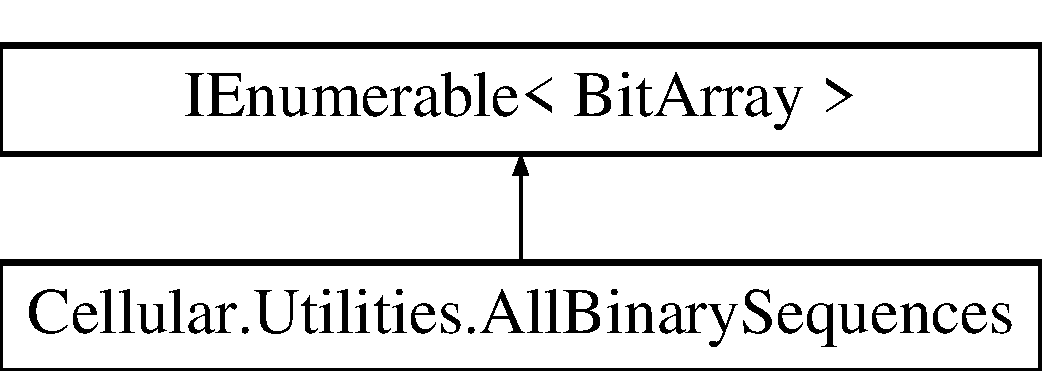
\includegraphics[height=2.000000cm]{class_cellular_1_1_utilities_1_1_all_binary_sequences}
\end{center}
\end{figure}
\subsection*{Public Member Functions}
\begin{DoxyCompactItemize}
\item 
\hyperlink{class_cellular_1_1_utilities_1_1_all_binary_sequences_adb657130e38906af075a17acf6e16364}{All\+Binary\+Sequences} (int sequence\+Length)
\begin{DoxyCompactList}\small\item\em Constructor. The amount of generated sequences will be 2 $^\wedge$ {\ttfamily sequence\+Length}. \end{DoxyCompactList}\end{DoxyCompactItemize}


\subsection{Detailed Description}
Class for enumerating all binary sequences of a given length. Starting from 00...00, ending at 11...11. 



Definition at line 213 of file Utilities.\+cs.



\subsection{Constructor \& Destructor Documentation}
\hypertarget{class_cellular_1_1_utilities_1_1_all_binary_sequences_adb657130e38906af075a17acf6e16364}{}\index{Cellular\+::\+Utilities\+::\+All\+Binary\+Sequences@{Cellular\+::\+Utilities\+::\+All\+Binary\+Sequences}!All\+Binary\+Sequences@{All\+Binary\+Sequences}}
\index{All\+Binary\+Sequences@{All\+Binary\+Sequences}!Cellular\+::\+Utilities\+::\+All\+Binary\+Sequences@{Cellular\+::\+Utilities\+::\+All\+Binary\+Sequences}}
\subsubsection[{All\+Binary\+Sequences(int sequence\+Length)}]{\setlength{\rightskip}{0pt plus 5cm}Cellular.\+Utilities.\+All\+Binary\+Sequences.\+All\+Binary\+Sequences (
\begin{DoxyParamCaption}
\item[{int}]{sequence\+Length}
\end{DoxyParamCaption}
)}\label{class_cellular_1_1_utilities_1_1_all_binary_sequences_adb657130e38906af075a17acf6e16364}


Constructor. The amount of generated sequences will be 2 $^\wedge$ {\ttfamily sequence\+Length}. 


\begin{DoxyParams}{Parameters}
{\em sequence\+Length} & \\
\hline
\end{DoxyParams}


Definition at line 221 of file Utilities.\+cs.



The documentation for this class was generated from the following file\+:\begin{DoxyCompactItemize}
\item 
C\+:/\+Martin/\+M\+F\+F/\+\_\+baka/\+Martin\+Dvorak/\+Cellular/\hyperlink{_utilities_8cs}{Utilities.\+cs}\end{DoxyCompactItemize}

\hypertarget{class_testing_1_1_automata_test}{}\section{Testing.\+Automata\+Test Class Reference}
\label{class_testing_1_1_automata_test}\index{Testing.\+Automata\+Test@{Testing.\+Automata\+Test}}
\subsection*{Static Public Member Functions}
\begin{DoxyCompactItemize}
\item 
static void \hyperlink{class_testing_1_1_automata_test_af2f191248a6d772c93fba9306fca092b}{Run\+Test} ()
\end{DoxyCompactItemize}


\subsection{Detailed Description}


Definition at line 6 of file Automata\+Test.\+cs.



\subsection{Member Function Documentation}
\hypertarget{class_testing_1_1_automata_test_af2f191248a6d772c93fba9306fca092b}{}\index{Testing\+::\+Automata\+Test@{Testing\+::\+Automata\+Test}!Run\+Test@{Run\+Test}}
\index{Run\+Test@{Run\+Test}!Testing\+::\+Automata\+Test@{Testing\+::\+Automata\+Test}}
\subsubsection[{Run\+Test()}]{\setlength{\rightskip}{0pt plus 5cm}static void Testing.\+Automata\+Test.\+Run\+Test (
\begin{DoxyParamCaption}
{}
\end{DoxyParamCaption}
)\hspace{0.3cm}{\ttfamily [static]}}\label{class_testing_1_1_automata_test_af2f191248a6d772c93fba9306fca092b}


Definition at line 8 of file Automata\+Test.\+cs.



The documentation for this class was generated from the following file\+:\begin{DoxyCompactItemize}
\item 
C\+:/\+Martin/\+M\+F\+F/\+\_\+baka/\+Martin\+Dvorak/\+Testing/\hyperlink{_automata_test_8cs}{Automata\+Test.\+cs}\end{DoxyCompactItemize}

\hypertarget{class_cellular_1_1_automaton1_d}{}\section{Cellular.\+Automaton1\+D Class Reference}
\label{class_cellular_1_1_automaton1_d}\index{Cellular.\+Automaton1\+D@{Cellular.\+Automaton1\+D}}


Abstract class for all 1\+D automata (binary \& others).  


Inheritance diagram for Cellular.\+Automaton1\+D\+:\begin{figure}[H]
\begin{center}
\leavevmode
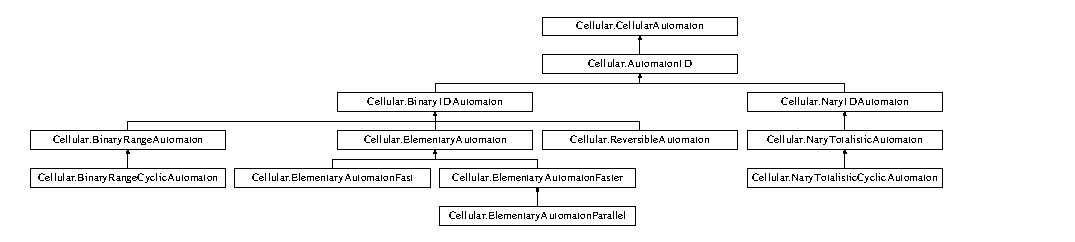
\includegraphics[height=2.916667cm]{class_cellular_1_1_automaton1_d}
\end{center}
\end{figure}
\subsection*{Protected Attributes}
\begin{DoxyCompactItemize}
\item 
int \hyperlink{class_cellular_1_1_automaton1_d_a915129ccf0f1e7092844c99ce6a28e5b}{size}
\end{DoxyCompactItemize}
\subsection*{Additional Inherited Members}


\subsection{Detailed Description}
Abstract class for all 1\+D automata (binary \& others). 



Definition at line 6 of file Automaton1\+D.\+cs.



\subsection{Member Data Documentation}
\hypertarget{class_cellular_1_1_automaton1_d_a915129ccf0f1e7092844c99ce6a28e5b}{}\index{Cellular\+::\+Automaton1\+D@{Cellular\+::\+Automaton1\+D}!size@{size}}
\index{size@{size}!Cellular\+::\+Automaton1\+D@{Cellular\+::\+Automaton1\+D}}
\subsubsection[{size}]{\setlength{\rightskip}{0pt plus 5cm}int Cellular.\+Automaton1\+D.\+size\hspace{0.3cm}{\ttfamily [protected]}}\label{class_cellular_1_1_automaton1_d_a915129ccf0f1e7092844c99ce6a28e5b}


Definition at line 8 of file Automaton1\+D.\+cs.



The documentation for this class was generated from the following file\+:\begin{DoxyCompactItemize}
\item 
C\+:/\+Martin/\+M\+F\+F/\+\_\+baka/\+Martin\+Dvorak/\+Cellular/\hyperlink{_automaton1_d_8cs}{Automaton1\+D.\+cs}\end{DoxyCompactItemize}

\hypertarget{class_cellular_1_1_automaton2_d}{}\section{Cellular.\+Automaton2\+D Class Reference}
\label{class_cellular_1_1_automaton2_d}\index{Cellular.\+Automaton2\+D@{Cellular.\+Automaton2\+D}}


Abstract class for all 2\+D automata. When indexing, (\char`\"{}height first\char`\"{}) the distance from the top comes before the distance from the left border.  


Inheritance diagram for Cellular.\+Automaton2\+D\+:\begin{figure}[H]
\begin{center}
\leavevmode
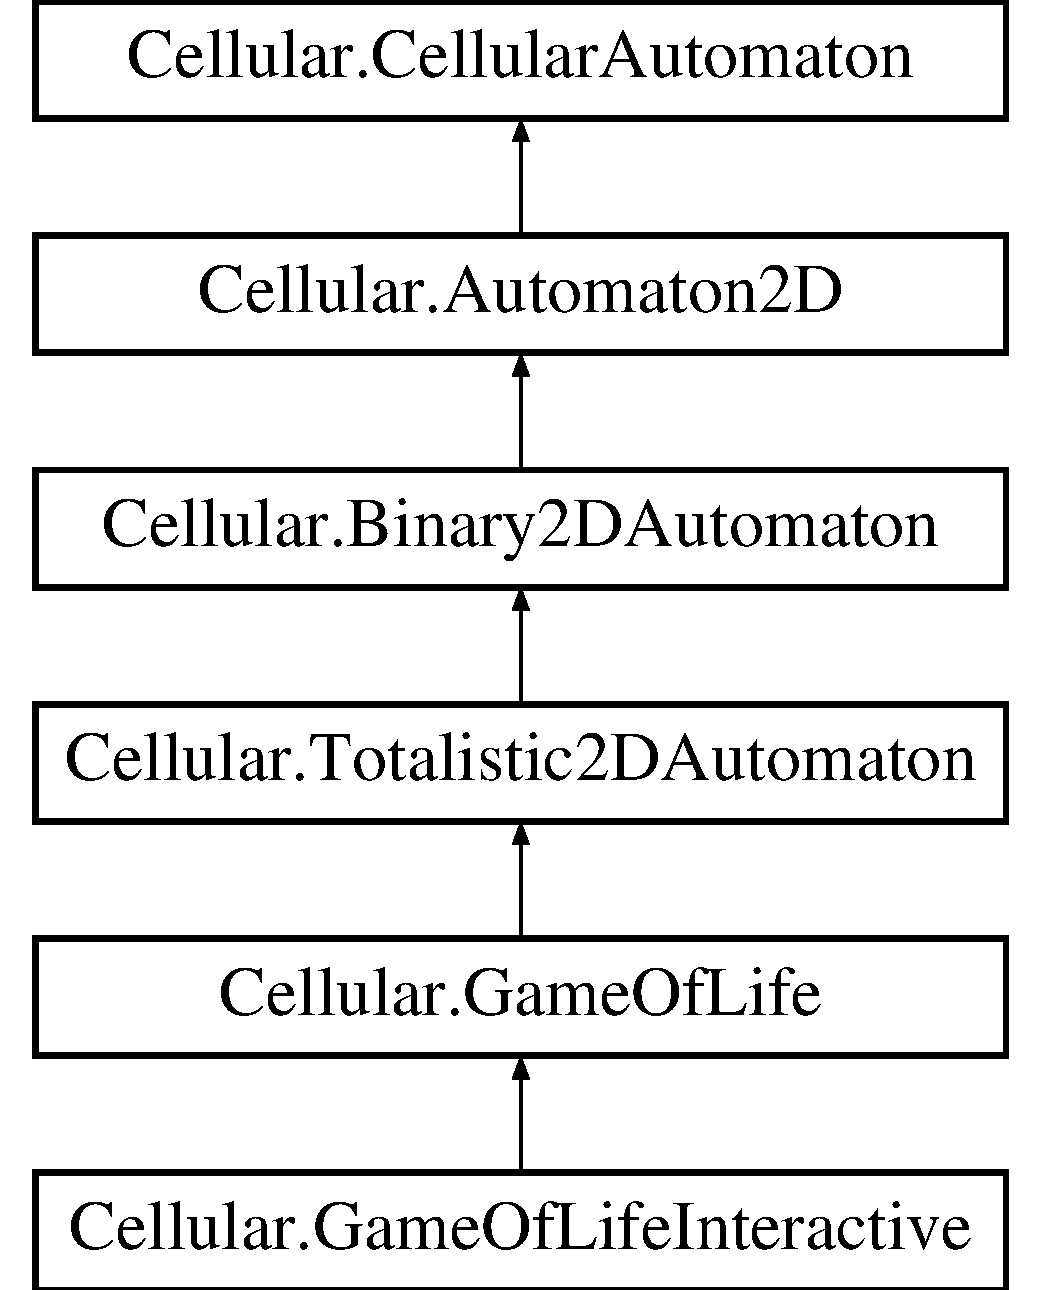
\includegraphics[height=5.000000cm]{class_cellular_1_1_automaton2_d}
\end{center}
\end{figure}
\subsection*{Protected Attributes}
\begin{DoxyCompactItemize}
\item 
int \hyperlink{class_cellular_1_1_automaton2_d_a1e9e5ec637c747a859c346839c90d174}{width}
\end{DoxyCompactItemize}
\subsection*{Additional Inherited Members}


\subsection{Detailed Description}
Abstract class for all 2\+D automata. When indexing, (\char`\"{}height first\char`\"{}) the distance from the top comes before the distance from the left border. 



Definition at line 7 of file Automaton2\+D.\+cs.



\subsection{Member Data Documentation}
\hypertarget{class_cellular_1_1_automaton2_d_a1e9e5ec637c747a859c346839c90d174}{}\index{Cellular\+::\+Automaton2\+D@{Cellular\+::\+Automaton2\+D}!width@{width}}
\index{width@{width}!Cellular\+::\+Automaton2\+D@{Cellular\+::\+Automaton2\+D}}
\subsubsection[{width}]{\setlength{\rightskip}{0pt plus 5cm}int Cellular.\+Automaton2\+D.\+width\hspace{0.3cm}{\ttfamily [protected]}}\label{class_cellular_1_1_automaton2_d_a1e9e5ec637c747a859c346839c90d174}


Definition at line 9 of file Automaton2\+D.\+cs.



The documentation for this class was generated from the following file\+:\begin{DoxyCompactItemize}
\item 
C\+:/\+Martin/\+M\+F\+F/\+\_\+baka/\+Martin\+Dvorak/\+Cellular/\hyperlink{_automaton2_d_8cs}{Automaton2\+D.\+cs}\end{DoxyCompactItemize}

\hypertarget{class_cellular_1_1_binary1_d_automaton}{}\section{Cellular.\+Binary1\+D\+Automaton Class Reference}
\label{class_cellular_1_1_binary1_d_automaton}\index{Cellular.\+Binary1\+D\+Automaton@{Cellular.\+Binary1\+D\+Automaton}}


Class containing base-\/constructors for all binary 1\+D automata and implementation of the {\ttfamily \hyperlink{interface_cellular_1_1_i_binary_c_a}{I\+Binary\+C\+A}} interface. The state is kept in a {\ttfamily Bit\+Array}.  


Inheritance diagram for Cellular.\+Binary1\+D\+Automaton\+:\begin{figure}[H]
\begin{center}
\leavevmode
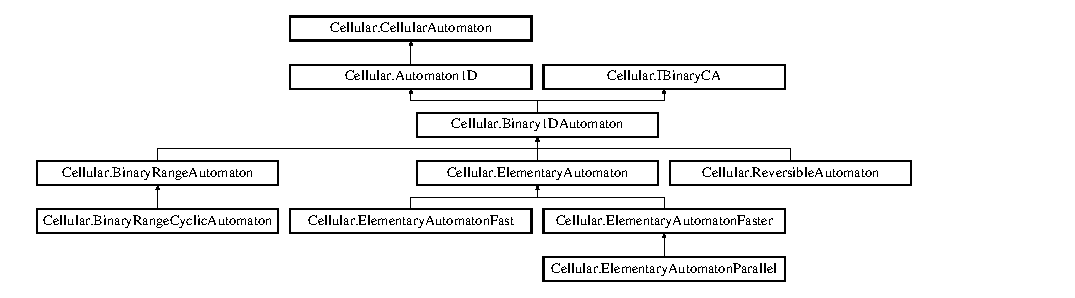
\includegraphics[height=3.954802cm]{class_cellular_1_1_binary1_d_automaton}
\end{center}
\end{figure}
\subsection*{Public Member Functions}
\begin{DoxyCompactItemize}
\item 
\hyperlink{class_cellular_1_1_binary1_d_automaton_a430f4985d036b8e48bfc785fe57b2bd1}{Binary1\+D\+Automaton} (int \hyperlink{class_cellular_1_1_automaton1_d_a915129ccf0f1e7092844c99ce6a28e5b}{size})
\begin{DoxyCompactList}\small\item\em Creates a new {\ttfamily \hyperlink{class_cellular_1_1_binary1_d_automaton}{Binary1\+D\+Automaton}} of given size with 000...00100...000 as its initial state. \end{DoxyCompactList}\item 
\hyperlink{class_cellular_1_1_binary1_d_automaton_a5c20fa6b3f7ffdd92187d216929099d4}{Binary1\+D\+Automaton} (Bit\+Array \hyperlink{all__1_8js_ae8b87ff4be2ae1dd5267342795263360}{initial\+State})
\begin{DoxyCompactList}\small\item\em Creates a new {\ttfamily \hyperlink{class_cellular_1_1_binary1_d_automaton}{Binary1\+D\+Automaton}} of given initial state. \end{DoxyCompactList}\item 
\hyperlink{class_cellular_1_1_binary1_d_automaton_af4e1fb39b1b0dad8c3ab648c7ba0ba8c}{Binary1\+D\+Automaton} (int \hyperlink{class_cellular_1_1_automaton1_d_a915129ccf0f1e7092844c99ce6a28e5b}{size}, Random rnd)
\begin{DoxyCompactList}\small\item\em Creates a new {\ttfamily \hyperlink{class_cellular_1_1_binary1_d_automaton}{Binary1\+D\+Automaton}} of given size with a random initial state. \end{DoxyCompactList}\item 
override int \hyperlink{class_cellular_1_1_binary1_d_automaton_add2d1cf0d8d25af3ac4af819be2561b9}{Get\+Hash\+Code} ()
\end{DoxyCompactItemize}
\subsection*{Protected Member Functions}
\begin{DoxyCompactItemize}
\item 
abstract \hyperlink{interface_cellular_1_1_i_binary_c_a}{I\+Binary\+C\+A} \hyperlink{class_cellular_1_1_binary1_d_automaton_a38ac5ae077c5d31356d278247fbab40a}{clone\+Template} (Bit\+Array new\+Instance\+State)
\end{DoxyCompactItemize}
\subsection*{Protected Attributes}
\begin{DoxyCompactItemize}
\item 
Bit\+Array \hyperlink{class_cellular_1_1_binary1_d_automaton_a5614d8d37b2511f69d8ae1a8ff0d8d73}{state}
\end{DoxyCompactItemize}


\subsection{Detailed Description}
Class containing base-\/constructors for all binary 1\+D automata and implementation of the {\ttfamily \hyperlink{interface_cellular_1_1_i_binary_c_a}{I\+Binary\+C\+A}} interface. The state is kept in a {\ttfamily Bit\+Array}. 



Definition at line 11 of file Binary1\+D\+Automaton.\+cs.



\subsection{Constructor \& Destructor Documentation}
\hypertarget{class_cellular_1_1_binary1_d_automaton_a430f4985d036b8e48bfc785fe57b2bd1}{}\index{Cellular\+::\+Binary1\+D\+Automaton@{Cellular\+::\+Binary1\+D\+Automaton}!Binary1\+D\+Automaton@{Binary1\+D\+Automaton}}
\index{Binary1\+D\+Automaton@{Binary1\+D\+Automaton}!Cellular\+::\+Binary1\+D\+Automaton@{Cellular\+::\+Binary1\+D\+Automaton}}
\subsubsection[{Binary1\+D\+Automaton(int size)}]{\setlength{\rightskip}{0pt plus 5cm}Cellular.\+Binary1\+D\+Automaton.\+Binary1\+D\+Automaton (
\begin{DoxyParamCaption}
\item[{int}]{size}
\end{DoxyParamCaption}
)}\label{class_cellular_1_1_binary1_d_automaton_a430f4985d036b8e48bfc785fe57b2bd1}


Creates a new {\ttfamily \hyperlink{class_cellular_1_1_binary1_d_automaton}{Binary1\+D\+Automaton}} of given size with 000...00100...000 as its initial state. 


\begin{DoxyParams}{Parameters}
{\em size} & The size of the new C\+A.\\
\hline
\end{DoxyParams}


Definition at line 19 of file Binary1\+D\+Automaton.\+cs.

\hypertarget{class_cellular_1_1_binary1_d_automaton_a5c20fa6b3f7ffdd92187d216929099d4}{}\index{Cellular\+::\+Binary1\+D\+Automaton@{Cellular\+::\+Binary1\+D\+Automaton}!Binary1\+D\+Automaton@{Binary1\+D\+Automaton}}
\index{Binary1\+D\+Automaton@{Binary1\+D\+Automaton}!Cellular\+::\+Binary1\+D\+Automaton@{Cellular\+::\+Binary1\+D\+Automaton}}
\subsubsection[{Binary1\+D\+Automaton(\+Bit\+Array initial\+State)}]{\setlength{\rightskip}{0pt plus 5cm}Cellular.\+Binary1\+D\+Automaton.\+Binary1\+D\+Automaton (
\begin{DoxyParamCaption}
\item[{Bit\+Array}]{initial\+State}
\end{DoxyParamCaption}
)}\label{class_cellular_1_1_binary1_d_automaton_a5c20fa6b3f7ffdd92187d216929099d4}


Creates a new {\ttfamily \hyperlink{class_cellular_1_1_binary1_d_automaton}{Binary1\+D\+Automaton}} of given initial state. 


\begin{DoxyParams}{Parameters}
{\em initial\+State} & A {\ttfamily Bit\+Array} describing the initial state of the C\+A. This also determines the size of the new C\+A.\\
\hline
\end{DoxyParams}


Definition at line 31 of file Binary1\+D\+Automaton.\+cs.

\hypertarget{class_cellular_1_1_binary1_d_automaton_af4e1fb39b1b0dad8c3ab648c7ba0ba8c}{}\index{Cellular\+::\+Binary1\+D\+Automaton@{Cellular\+::\+Binary1\+D\+Automaton}!Binary1\+D\+Automaton@{Binary1\+D\+Automaton}}
\index{Binary1\+D\+Automaton@{Binary1\+D\+Automaton}!Cellular\+::\+Binary1\+D\+Automaton@{Cellular\+::\+Binary1\+D\+Automaton}}
\subsubsection[{Binary1\+D\+Automaton(int size, Random rnd)}]{\setlength{\rightskip}{0pt plus 5cm}Cellular.\+Binary1\+D\+Automaton.\+Binary1\+D\+Automaton (
\begin{DoxyParamCaption}
\item[{int}]{size, }
\item[{Random}]{rnd}
\end{DoxyParamCaption}
)}\label{class_cellular_1_1_binary1_d_automaton_af4e1fb39b1b0dad8c3ab648c7ba0ba8c}


Creates a new {\ttfamily \hyperlink{class_cellular_1_1_binary1_d_automaton}{Binary1\+D\+Automaton}} of given size with a random initial state. 


\begin{DoxyParams}{Parameters}
{\em size} & The size of the new C\+A.\\
\hline
{\em rnd} & Pseudo\+R\+N\+G instance that will be used to generate the original state.\\
\hline
\end{DoxyParams}


Definition at line 42 of file Binary1\+D\+Automaton.\+cs.



\subsection{Member Function Documentation}
\hypertarget{class_cellular_1_1_binary1_d_automaton_a38ac5ae077c5d31356d278247fbab40a}{}\index{Cellular\+::\+Binary1\+D\+Automaton@{Cellular\+::\+Binary1\+D\+Automaton}!clone\+Template@{clone\+Template}}
\index{clone\+Template@{clone\+Template}!Cellular\+::\+Binary1\+D\+Automaton@{Cellular\+::\+Binary1\+D\+Automaton}}
\subsubsection[{clone\+Template(\+Bit\+Array new\+Instance\+State)}]{\setlength{\rightskip}{0pt plus 5cm}abstract {\bf I\+Binary\+C\+A} Cellular.\+Binary1\+D\+Automaton.\+clone\+Template (
\begin{DoxyParamCaption}
\item[{Bit\+Array}]{new\+Instance\+State}
\end{DoxyParamCaption}
)\hspace{0.3cm}{\ttfamily [protected]}, {\ttfamily [pure virtual]}}\label{class_cellular_1_1_binary1_d_automaton_a38ac5ae077c5d31356d278247fbab40a}


Implemented in \hyperlink{class_cellular_1_1_elementary_fast_automaton_a95b5abc22d134cb9640b56a0a70c1454}{Cellular.\+Elementary\+Fast\+Automaton}, \hyperlink{class_cellular_1_1_binary_range_automaton_a75d9e1fc19f9bfc470e66b12aaf1abe8}{Cellular.\+Binary\+Range\+Automaton}, \hyperlink{class_cellular_1_1_elementary_automaton_ae2a263ffe6e021daff6a4a6c45555f6c}{Cellular.\+Elementary\+Automaton}, \hyperlink{class_cellular_1_1_reversible_automaton_ab2a93e95a7428b1899623975cf6615c5}{Cellular.\+Reversible\+Automaton}, and \hyperlink{class_cellular_1_1_binary_range_cyclic_automaton_a38ebc4d1f2610701299106475229c60b}{Cellular.\+Binary\+Range\+Cyclic\+Automaton}.

\hypertarget{class_cellular_1_1_binary1_d_automaton_add2d1cf0d8d25af3ac4af819be2561b9}{}\index{Cellular\+::\+Binary1\+D\+Automaton@{Cellular\+::\+Binary1\+D\+Automaton}!Get\+Hash\+Code@{Get\+Hash\+Code}}
\index{Get\+Hash\+Code@{Get\+Hash\+Code}!Cellular\+::\+Binary1\+D\+Automaton@{Cellular\+::\+Binary1\+D\+Automaton}}
\subsubsection[{Get\+Hash\+Code()}]{\setlength{\rightskip}{0pt plus 5cm}override int Cellular.\+Binary1\+D\+Automaton.\+Get\+Hash\+Code (
\begin{DoxyParamCaption}
{}
\end{DoxyParamCaption}
)}\label{class_cellular_1_1_binary1_d_automaton_add2d1cf0d8d25af3ac4af819be2561b9}


Definition at line 92 of file Binary1\+D\+Automaton.\+cs.



\subsection{Member Data Documentation}
\hypertarget{class_cellular_1_1_binary1_d_automaton_a5614d8d37b2511f69d8ae1a8ff0d8d73}{}\index{Cellular\+::\+Binary1\+D\+Automaton@{Cellular\+::\+Binary1\+D\+Automaton}!state@{state}}
\index{state@{state}!Cellular\+::\+Binary1\+D\+Automaton@{Cellular\+::\+Binary1\+D\+Automaton}}
\subsubsection[{state}]{\setlength{\rightskip}{0pt plus 5cm}Bit\+Array Cellular.\+Binary1\+D\+Automaton.\+state\hspace{0.3cm}{\ttfamily [protected]}}\label{class_cellular_1_1_binary1_d_automaton_a5614d8d37b2511f69d8ae1a8ff0d8d73}


Definition at line 13 of file Binary1\+D\+Automaton.\+cs.



The documentation for this class was generated from the following file\+:\begin{DoxyCompactItemize}
\item 
C\+:/\+Martin/\+M\+F\+F/\+\_\+baka/\+Martin\+Dvorak/\+Cellular/\hyperlink{_binary1_d_automaton_8cs}{Binary1\+D\+Automaton.\+cs}\end{DoxyCompactItemize}

\hypertarget{class_cellular_1_1_binary2_d_automaton}{}\section{Cellular.\+Binary2\+D\+Automaton Class Reference}
\label{class_cellular_1_1_binary2_d_automaton}\index{Cellular.\+Binary2\+D\+Automaton@{Cellular.\+Binary2\+D\+Automaton}}


Class containing base-\/constructors for all binary 2\+D automata and implementation of the {\ttfamily \hyperlink{interface_cellular_1_1_i_binary_c_a}{I\+Binary\+C\+A}} interface. The state is kept in an array of {\ttfamily Bit\+Array}s reprezenting rows.  


Inheritance diagram for Cellular.\+Binary2\+D\+Automaton\+:\begin{figure}[H]
\begin{center}
\leavevmode
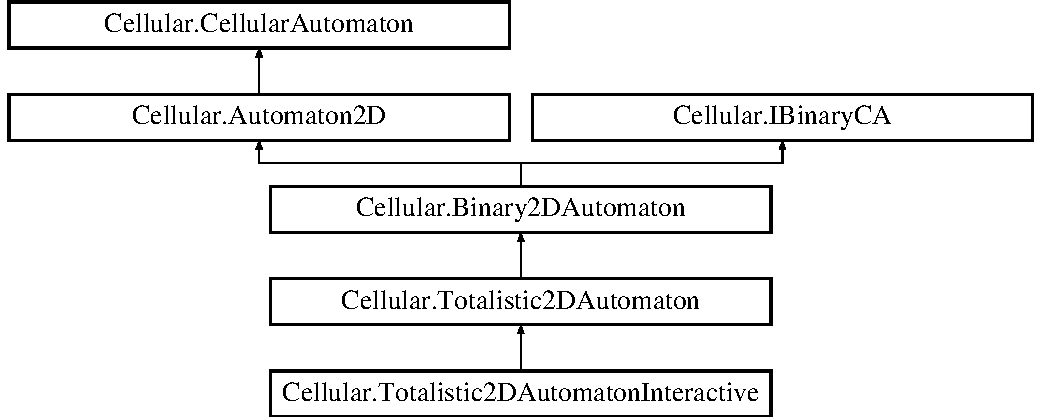
\includegraphics[height=5.000000cm]{class_cellular_1_1_binary2_d_automaton}
\end{center}
\end{figure}
\subsection*{Public Member Functions}
\begin{DoxyCompactItemize}
\item 
\hyperlink{class_cellular_1_1_binary2_d_automaton_a6956aa8cc05e4d00c116d8cc5e8528d4}{Binary2\+D\+Automaton} (int \hyperlink{class_cellular_1_1_automaton2_d_a1e9e5ec637c747a859c346839c90d174}{width}, int height)
\begin{DoxyCompactList}\small\item\em Creates a new {\ttfamily \hyperlink{class_cellular_1_1_binary2_d_automaton}{Binary2\+D\+Automaton}} of given size with one living cell in the middle, the rest is dead. \end{DoxyCompactList}\item 
\hyperlink{class_cellular_1_1_binary2_d_automaton_ab2bdc13f759e29b0efe84995c74e5006}{Binary2\+D\+Automaton} (Bit\+Array\mbox{[}$\,$\mbox{]} \hyperlink{all__1_8js_ae8b87ff4be2ae1dd5267342795263360}{initial\+State})
\begin{DoxyCompactList}\small\item\em Creates a new {\ttfamily \hyperlink{class_cellular_1_1_binary2_d_automaton}{Binary2\+D\+Automaton}} of given initial state. \end{DoxyCompactList}\item 
\hyperlink{class_cellular_1_1_binary2_d_automaton_a465d87aeab9f265595e942e46308f75f}{Binary2\+D\+Automaton} (int \hyperlink{class_cellular_1_1_automaton2_d_a1e9e5ec637c747a859c346839c90d174}{width}, int height, Random rnd)
\begin{DoxyCompactList}\small\item\em Creates a new {\ttfamily \hyperlink{class_cellular_1_1_binary2_d_automaton}{Binary2\+D\+Automaton}} of given size with a random initial state. \end{DoxyCompactList}\item 
override int \hyperlink{class_cellular_1_1_binary2_d_automaton_af0b06d58b66367dbeb712f2c4237ff54}{Get\+Hash\+Code} ()
\end{DoxyCompactItemize}
\subsection*{Protected Member Functions}
\begin{DoxyCompactItemize}
\item 
abstract \hyperlink{interface_cellular_1_1_i_binary_c_a}{I\+Binary\+C\+A} \hyperlink{class_cellular_1_1_binary2_d_automaton_ad2d31668c7b8f8e959575e03b995273f}{clone\+Template} (Bit\+Array\mbox{[}$\,$\mbox{]} new\+Instance\+State)
\end{DoxyCompactItemize}
\subsection*{Protected Attributes}
\begin{DoxyCompactItemize}
\item 
Bit\+Array\mbox{[}$\,$\mbox{]} \hyperlink{class_cellular_1_1_binary2_d_automaton_abac140afbe1d9263ef35aa596c181407}{state}
\end{DoxyCompactItemize}


\subsection{Detailed Description}
Class containing base-\/constructors for all binary 2\+D automata and implementation of the {\ttfamily \hyperlink{interface_cellular_1_1_i_binary_c_a}{I\+Binary\+C\+A}} interface. The state is kept in an array of {\ttfamily Bit\+Array}s reprezenting rows. 



Definition at line 11 of file Binary2\+D\+Automaton.\+cs.



\subsection{Constructor \& Destructor Documentation}
\hypertarget{class_cellular_1_1_binary2_d_automaton_a6956aa8cc05e4d00c116d8cc5e8528d4}{}\index{Cellular\+::\+Binary2\+D\+Automaton@{Cellular\+::\+Binary2\+D\+Automaton}!Binary2\+D\+Automaton@{Binary2\+D\+Automaton}}
\index{Binary2\+D\+Automaton@{Binary2\+D\+Automaton}!Cellular\+::\+Binary2\+D\+Automaton@{Cellular\+::\+Binary2\+D\+Automaton}}
\subsubsection[{Binary2\+D\+Automaton(int width, int height)}]{\setlength{\rightskip}{0pt plus 5cm}Cellular.\+Binary2\+D\+Automaton.\+Binary2\+D\+Automaton (
\begin{DoxyParamCaption}
\item[{int}]{width, }
\item[{int}]{height}
\end{DoxyParamCaption}
)}\label{class_cellular_1_1_binary2_d_automaton_a6956aa8cc05e4d00c116d8cc5e8528d4}


Creates a new {\ttfamily \hyperlink{class_cellular_1_1_binary2_d_automaton}{Binary2\+D\+Automaton}} of given size with one living cell in the middle, the rest is dead. 


\begin{DoxyParams}{Parameters}
{\em width} & The width of the new C\+A (length of rows).\\
\hline
{\em height} & The height of the new C\+A (number of rows).\\
\hline
\end{DoxyParams}


Definition at line 20 of file Binary2\+D\+Automaton.\+cs.

\hypertarget{class_cellular_1_1_binary2_d_automaton_ab2bdc13f759e29b0efe84995c74e5006}{}\index{Cellular\+::\+Binary2\+D\+Automaton@{Cellular\+::\+Binary2\+D\+Automaton}!Binary2\+D\+Automaton@{Binary2\+D\+Automaton}}
\index{Binary2\+D\+Automaton@{Binary2\+D\+Automaton}!Cellular\+::\+Binary2\+D\+Automaton@{Cellular\+::\+Binary2\+D\+Automaton}}
\subsubsection[{Binary2\+D\+Automaton(\+Bit\+Array[] initial\+State)}]{\setlength{\rightskip}{0pt plus 5cm}Cellular.\+Binary2\+D\+Automaton.\+Binary2\+D\+Automaton (
\begin{DoxyParamCaption}
\item[{Bit\+Array\mbox{[}$\,$\mbox{]}}]{initial\+State}
\end{DoxyParamCaption}
)}\label{class_cellular_1_1_binary2_d_automaton_ab2bdc13f759e29b0efe84995c74e5006}


Creates a new {\ttfamily \hyperlink{class_cellular_1_1_binary2_d_automaton}{Binary2\+D\+Automaton}} of given initial state. 


\begin{DoxyParams}{Parameters}
{\em initial\+State} & An array of {\ttfamily Bit\+Array}s describing the initial state of the C\+A. This also determines the size (width, height) of the new C\+A.\\
\hline
\end{DoxyParams}


Definition at line 37 of file Binary2\+D\+Automaton.\+cs.

\hypertarget{class_cellular_1_1_binary2_d_automaton_a465d87aeab9f265595e942e46308f75f}{}\index{Cellular\+::\+Binary2\+D\+Automaton@{Cellular\+::\+Binary2\+D\+Automaton}!Binary2\+D\+Automaton@{Binary2\+D\+Automaton}}
\index{Binary2\+D\+Automaton@{Binary2\+D\+Automaton}!Cellular\+::\+Binary2\+D\+Automaton@{Cellular\+::\+Binary2\+D\+Automaton}}
\subsubsection[{Binary2\+D\+Automaton(int width, int height, Random rnd)}]{\setlength{\rightskip}{0pt plus 5cm}Cellular.\+Binary2\+D\+Automaton.\+Binary2\+D\+Automaton (
\begin{DoxyParamCaption}
\item[{int}]{width, }
\item[{int}]{height, }
\item[{Random}]{rnd}
\end{DoxyParamCaption}
)}\label{class_cellular_1_1_binary2_d_automaton_a465d87aeab9f265595e942e46308f75f}


Creates a new {\ttfamily \hyperlink{class_cellular_1_1_binary2_d_automaton}{Binary2\+D\+Automaton}} of given size with a random initial state. 


\begin{DoxyParams}{Parameters}
{\em width} & The width of the new C\+A (length of rows).\\
\hline
{\em height} & The height of the new C\+A (number of rows).\\
\hline
{\em rnd} & Pseudo\+R\+N\+G instance that will be used to generate the original state.\\
\hline
\end{DoxyParams}


Definition at line 50 of file Binary2\+D\+Automaton.\+cs.



\subsection{Member Function Documentation}
\hypertarget{class_cellular_1_1_binary2_d_automaton_ad2d31668c7b8f8e959575e03b995273f}{}\index{Cellular\+::\+Binary2\+D\+Automaton@{Cellular\+::\+Binary2\+D\+Automaton}!clone\+Template@{clone\+Template}}
\index{clone\+Template@{clone\+Template}!Cellular\+::\+Binary2\+D\+Automaton@{Cellular\+::\+Binary2\+D\+Automaton}}
\subsubsection[{clone\+Template(\+Bit\+Array[] new\+Instance\+State)}]{\setlength{\rightskip}{0pt plus 5cm}abstract {\bf I\+Binary\+C\+A} Cellular.\+Binary2\+D\+Automaton.\+clone\+Template (
\begin{DoxyParamCaption}
\item[{Bit\+Array\mbox{[}$\,$\mbox{]}}]{new\+Instance\+State}
\end{DoxyParamCaption}
)\hspace{0.3cm}{\ttfamily [protected]}, {\ttfamily [pure virtual]}}\label{class_cellular_1_1_binary2_d_automaton_ad2d31668c7b8f8e959575e03b995273f}


Implemented in \hyperlink{class_cellular_1_1_totalistic2_d_automaton_ad5cc3f46a556aa1b1c99bdfa92f5ba1d}{Cellular.\+Totalistic2\+D\+Automaton}.

\hypertarget{class_cellular_1_1_binary2_d_automaton_af0b06d58b66367dbeb712f2c4237ff54}{}\index{Cellular\+::\+Binary2\+D\+Automaton@{Cellular\+::\+Binary2\+D\+Automaton}!Get\+Hash\+Code@{Get\+Hash\+Code}}
\index{Get\+Hash\+Code@{Get\+Hash\+Code}!Cellular\+::\+Binary2\+D\+Automaton@{Cellular\+::\+Binary2\+D\+Automaton}}
\subsubsection[{Get\+Hash\+Code()}]{\setlength{\rightskip}{0pt plus 5cm}override int Cellular.\+Binary2\+D\+Automaton.\+Get\+Hash\+Code (
\begin{DoxyParamCaption}
{}
\end{DoxyParamCaption}
)}\label{class_cellular_1_1_binary2_d_automaton_af0b06d58b66367dbeb712f2c4237ff54}


Definition at line 158 of file Binary2\+D\+Automaton.\+cs.



\subsection{Member Data Documentation}
\hypertarget{class_cellular_1_1_binary2_d_automaton_abac140afbe1d9263ef35aa596c181407}{}\index{Cellular\+::\+Binary2\+D\+Automaton@{Cellular\+::\+Binary2\+D\+Automaton}!state@{state}}
\index{state@{state}!Cellular\+::\+Binary2\+D\+Automaton@{Cellular\+::\+Binary2\+D\+Automaton}}
\subsubsection[{state}]{\setlength{\rightskip}{0pt plus 5cm}Bit\+Array \mbox{[}$\,$\mbox{]} Cellular.\+Binary2\+D\+Automaton.\+state\hspace{0.3cm}{\ttfamily [protected]}}\label{class_cellular_1_1_binary2_d_automaton_abac140afbe1d9263ef35aa596c181407}


Definition at line 13 of file Binary2\+D\+Automaton.\+cs.



The documentation for this class was generated from the following file\+:\begin{DoxyCompactItemize}
\item 
C\+:/\+Martin/\+M\+F\+F/\+\_\+baka/\+Martin\+Dvorak/\+Cellular/\hyperlink{_binary2_d_automaton_8cs}{Binary2\+D\+Automaton.\+cs}\end{DoxyCompactItemize}

\hypertarget{class_cellular_1_1_binary_range_automaton}{}\section{Cellular.\+Binary\+Range\+Automaton Class Reference}
\label{class_cellular_1_1_binary_range_automaton}\index{Cellular.\+Binary\+Range\+Automaton@{Cellular.\+Binary\+Range\+Automaton}}


Class representing any binary 1\+D automaton with symmetric scope. The automaton has firmly set borders. Referencing a cell beyond borders acts as referencing a dead cell.  


Inheritance diagram for Cellular.\+Binary\+Range\+Automaton\+:\begin{figure}[H]
\begin{center}
\leavevmode
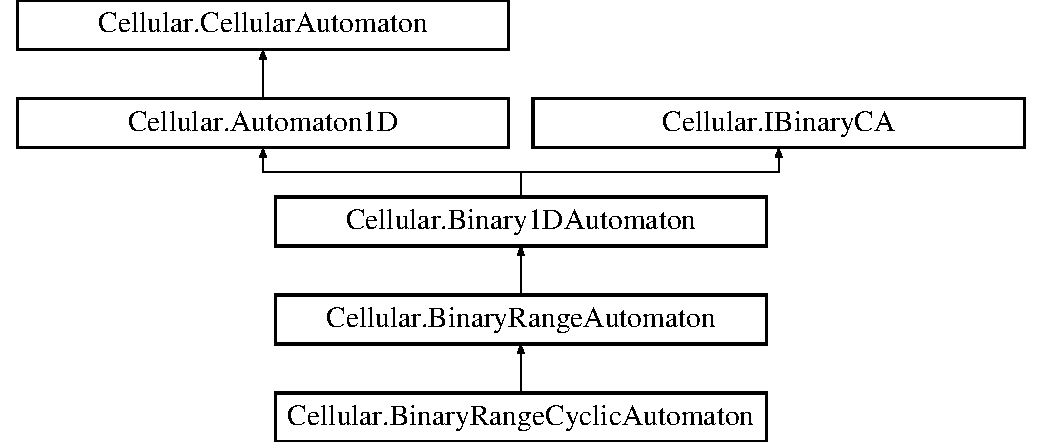
\includegraphics[height=5.000000cm]{class_cellular_1_1_binary_range_automaton}
\end{center}
\end{figure}
\subsection*{Public Member Functions}
\begin{DoxyCompactItemize}
\item 
\hyperlink{class_cellular_1_1_binary_range_automaton_a3b165a9e98e516bf7e9bdb8bb2fe16a7}{Binary\+Range\+Automaton} (byte scope, bool\mbox{[}$\,$\mbox{]} \hyperlink{class_cellular_1_1_binary_range_automaton_a4dda99c3151599c8ef12d08d7472144c}{rule}, int \hyperlink{class_cellular_1_1_automaton1_d_a915129ccf0f1e7092844c99ce6a28e5b}{size})
\begin{DoxyCompactList}\small\item\em Creates a new C\+A of a general rule with 000...00100...000 as its initial state. \end{DoxyCompactList}\item 
\hyperlink{class_cellular_1_1_binary_range_automaton_a704950c30ff58c587c8a717f9f2c839b}{Binary\+Range\+Automaton} (byte scope, bool\mbox{[}$\,$\mbox{]} \hyperlink{class_cellular_1_1_binary_range_automaton_a4dda99c3151599c8ef12d08d7472144c}{rule}, Bit\+Array initial\+State)
\begin{DoxyCompactList}\small\item\em Creates a new C\+A of a general rule with defined inital state. \end{DoxyCompactList}\item 
override void \hyperlink{class_cellular_1_1_binary_range_automaton_ade1f5b831b9676f04f835c33d245b9e2}{Step} ()
\begin{DoxyCompactList}\small\item\em Performs one step of the cellular automaton. Always calls \end{DoxyCompactList}\item 
override object \hyperlink{class_cellular_1_1_binary_range_automaton_a12f010562e04785e0a7efb113302687e}{Clone} ()
\begin{DoxyCompactList}\small\item\em Creates an appropriate copy of the C\+A. Its type and the specific rule are always preserved. However, the time (number of steps executed on the specific instance) is set back to 0. \end{DoxyCompactList}\item 
override string \hyperlink{class_cellular_1_1_binary_range_automaton_afad205eb4fea51efd63b063f96bfda5c}{Tell\+Type} ()
\begin{DoxyCompactList}\small\item\em Announces the runtime type of the C\+A including info about its rule. It serves for debugging purposes. \end{DoxyCompactList}\end{DoxyCompactItemize}
\subsection*{Protected Member Functions}
\begin{DoxyCompactItemize}
\item 
virtual bool \hyperlink{class_cellular_1_1_binary_range_automaton_a462f8b1d9b77966e14bb0160a4a06dca}{get\+Value\+At} (int index)
\begin{DoxyCompactList}\small\item\em This method simplifies boundary conditions. \end{DoxyCompactList}\item 
override \hyperlink{interface_cellular_1_1_i_binary_c_a}{I\+Binary\+C\+A} \hyperlink{class_cellular_1_1_binary_range_automaton_a75d9e1fc19f9bfc470e66b12aaf1abe8}{clone\+Template} (Bit\+Array new\+Instance\+State)
\end{DoxyCompactItemize}
\subsection*{Protected Attributes}
\begin{DoxyCompactItemize}
\item 
bool\mbox{[}$\,$\mbox{]} \hyperlink{class_cellular_1_1_binary_range_automaton_a4dda99c3151599c8ef12d08d7472144c}{rule}
\item 
byte \hyperlink{class_cellular_1_1_binary_range_automaton_a9a391c738dc7725aa66a52dca039a2f7}{range}
\end{DoxyCompactItemize}


\subsection{Detailed Description}
Class representing any binary 1\+D automaton with symmetric scope. The automaton has firmly set borders. Referencing a cell beyond borders acts as referencing a dead cell. 



Definition at line 10 of file Binary\+Range\+Automaton.\+cs.



\subsection{Constructor \& Destructor Documentation}
\hypertarget{class_cellular_1_1_binary_range_automaton_a3b165a9e98e516bf7e9bdb8bb2fe16a7}{}\index{Cellular\+::\+Binary\+Range\+Automaton@{Cellular\+::\+Binary\+Range\+Automaton}!Binary\+Range\+Automaton@{Binary\+Range\+Automaton}}
\index{Binary\+Range\+Automaton@{Binary\+Range\+Automaton}!Cellular\+::\+Binary\+Range\+Automaton@{Cellular\+::\+Binary\+Range\+Automaton}}
\subsubsection[{Binary\+Range\+Automaton(byte scope, bool[] rule, int size)}]{\setlength{\rightskip}{0pt plus 5cm}Cellular.\+Binary\+Range\+Automaton.\+Binary\+Range\+Automaton (
\begin{DoxyParamCaption}
\item[{byte}]{scope, }
\item[{bool\mbox{[}$\,$\mbox{]}}]{rule, }
\item[{int}]{size}
\end{DoxyParamCaption}
)}\label{class_cellular_1_1_binary_range_automaton_a3b165a9e98e516bf7e9bdb8bb2fe16a7}


Creates a new C\+A of a general rule with 000...00100...000 as its initial state. 


\begin{DoxyParams}{Parameters}
{\em scope} & How many cells on each side from the center determine the next state of the cell. Value 1 makes it equivalent to a {\ttfamily \hyperlink{class_cellular_1_1_elementary_automaton}{Elementary\+Automaton}} which has rule of size 8. Value 2 means that each new state of any cell depends on five total cells =$>$ size of rule must be 32.\\
\hline
{\em rule} & Array representing the rule for creating a new state. rule\mbox{[}0\mbox{]} is rule for 0..0, therefore opposite order to the rules of basic automata.\\
\hline
{\em size} & The size of the new C\+A.\\
\hline
\end{DoxyParams}


Definition at line 24 of file Binary\+Range\+Automaton.\+cs.

\hypertarget{class_cellular_1_1_binary_range_automaton_a704950c30ff58c587c8a717f9f2c839b}{}\index{Cellular\+::\+Binary\+Range\+Automaton@{Cellular\+::\+Binary\+Range\+Automaton}!Binary\+Range\+Automaton@{Binary\+Range\+Automaton}}
\index{Binary\+Range\+Automaton@{Binary\+Range\+Automaton}!Cellular\+::\+Binary\+Range\+Automaton@{Cellular\+::\+Binary\+Range\+Automaton}}
\subsubsection[{Binary\+Range\+Automaton(byte scope, bool[] rule, Bit\+Array initial\+State)}]{\setlength{\rightskip}{0pt plus 5cm}Cellular.\+Binary\+Range\+Automaton.\+Binary\+Range\+Automaton (
\begin{DoxyParamCaption}
\item[{byte}]{scope, }
\item[{bool\mbox{[}$\,$\mbox{]}}]{rule, }
\item[{Bit\+Array}]{initial\+State}
\end{DoxyParamCaption}
)}\label{class_cellular_1_1_binary_range_automaton_a704950c30ff58c587c8a717f9f2c839b}


Creates a new C\+A of a general rule with defined inital state. 


\begin{DoxyParams}{Parameters}
{\em scope} & How many cells on each side from the center determine the next state of the cell. Value 1 makes it equivalent to a {\ttfamily \hyperlink{class_cellular_1_1_elementary_automaton}{Elementary\+Automaton}} which has rule of size 8. Value 2 means that each new state of any cell depends on five total cells =$>$ size of rule must be 32.\\
\hline
{\em rule} & Array representing the rule for creating a new state. rule\mbox{[}0\mbox{]} is rule for 0..0, therefore opposite order to the rules of basic automata.\\
\hline
{\em initial\+State} & A {\ttfamily Bit\+Array} describing the initial state of the C\+A. This also determines the size of the new C\+A.\\
\hline
\end{DoxyParams}


Definition at line 39 of file Binary\+Range\+Automaton.\+cs.



\subsection{Member Function Documentation}
\hypertarget{class_cellular_1_1_binary_range_automaton_a12f010562e04785e0a7efb113302687e}{}\index{Cellular\+::\+Binary\+Range\+Automaton@{Cellular\+::\+Binary\+Range\+Automaton}!Clone@{Clone}}
\index{Clone@{Clone}!Cellular\+::\+Binary\+Range\+Automaton@{Cellular\+::\+Binary\+Range\+Automaton}}
\subsubsection[{Clone()}]{\setlength{\rightskip}{0pt plus 5cm}override object Cellular.\+Binary\+Range\+Automaton.\+Clone (
\begin{DoxyParamCaption}
{}
\end{DoxyParamCaption}
)\hspace{0.3cm}{\ttfamily [virtual]}}\label{class_cellular_1_1_binary_range_automaton_a12f010562e04785e0a7efb113302687e}


Creates an appropriate copy of the C\+A. Its type and the specific rule are always preserved. However, the time (number of steps executed on the specific instance) is set back to 0. 

\begin{DoxyReturn}{Returns}
A copy of the {\ttfamily \hyperlink{class_cellular_1_1_cellular_automaton}{Cellular\+Automaton}} as an {\ttfamily Object}
\end{DoxyReturn}


Implements \hyperlink{class_cellular_1_1_cellular_automaton_affd487b397cdbbbb1982815bbcd8e7d3}{Cellular.\+Cellular\+Automaton}.



Reimplemented in \hyperlink{class_cellular_1_1_binary_range_cyclic_automaton_a2361fe82802e372b24b8bec6a6135278}{Cellular.\+Binary\+Range\+Cyclic\+Automaton}.



Definition at line 105 of file Binary\+Range\+Automaton.\+cs.

\hypertarget{class_cellular_1_1_binary_range_automaton_a75d9e1fc19f9bfc470e66b12aaf1abe8}{}\index{Cellular\+::\+Binary\+Range\+Automaton@{Cellular\+::\+Binary\+Range\+Automaton}!clone\+Template@{clone\+Template}}
\index{clone\+Template@{clone\+Template}!Cellular\+::\+Binary\+Range\+Automaton@{Cellular\+::\+Binary\+Range\+Automaton}}
\subsubsection[{clone\+Template(\+Bit\+Array new\+Instance\+State)}]{\setlength{\rightskip}{0pt plus 5cm}override {\bf I\+Binary\+C\+A} Cellular.\+Binary\+Range\+Automaton.\+clone\+Template (
\begin{DoxyParamCaption}
\item[{Bit\+Array}]{new\+Instance\+State}
\end{DoxyParamCaption}
)\hspace{0.3cm}{\ttfamily [protected]}, {\ttfamily [virtual]}}\label{class_cellular_1_1_binary_range_automaton_a75d9e1fc19f9bfc470e66b12aaf1abe8}


Implements \hyperlink{class_cellular_1_1_binary1_d_automaton_a38ac5ae077c5d31356d278247fbab40a}{Cellular.\+Binary1\+D\+Automaton}.



Reimplemented in \hyperlink{class_cellular_1_1_binary_range_cyclic_automaton_a38ebc4d1f2610701299106475229c60b}{Cellular.\+Binary\+Range\+Cyclic\+Automaton}.



Definition at line 110 of file Binary\+Range\+Automaton.\+cs.

\hypertarget{class_cellular_1_1_binary_range_automaton_a462f8b1d9b77966e14bb0160a4a06dca}{}\index{Cellular\+::\+Binary\+Range\+Automaton@{Cellular\+::\+Binary\+Range\+Automaton}!get\+Value\+At@{get\+Value\+At}}
\index{get\+Value\+At@{get\+Value\+At}!Cellular\+::\+Binary\+Range\+Automaton@{Cellular\+::\+Binary\+Range\+Automaton}}
\subsubsection[{get\+Value\+At(int index)}]{\setlength{\rightskip}{0pt plus 5cm}virtual bool Cellular.\+Binary\+Range\+Automaton.\+get\+Value\+At (
\begin{DoxyParamCaption}
\item[{int}]{index}
\end{DoxyParamCaption}
)\hspace{0.3cm}{\ttfamily [protected]}, {\ttfamily [virtual]}}\label{class_cellular_1_1_binary_range_automaton_a462f8b1d9b77966e14bb0160a4a06dca}


This method simplifies boundary conditions. 


\begin{DoxyParams}{Parameters}
{\em index} & Zero-\/based index (which bit is required).\\
\hline
\end{DoxyParams}
\begin{DoxyReturn}{Returns}
One bit.
\end{DoxyReturn}


Reimplemented in \hyperlink{class_cellular_1_1_binary_range_cyclic_automaton_a0e4d7dd11fda253300ee9fc8adbc4d33}{Cellular.\+Binary\+Range\+Cyclic\+Automaton}.



Definition at line 62 of file Binary\+Range\+Automaton.\+cs.

\hypertarget{class_cellular_1_1_binary_range_automaton_ade1f5b831b9676f04f835c33d245b9e2}{}\index{Cellular\+::\+Binary\+Range\+Automaton@{Cellular\+::\+Binary\+Range\+Automaton}!Step@{Step}}
\index{Step@{Step}!Cellular\+::\+Binary\+Range\+Automaton@{Cellular\+::\+Binary\+Range\+Automaton}}
\subsubsection[{Step()}]{\setlength{\rightskip}{0pt plus 5cm}override void Cellular.\+Binary\+Range\+Automaton.\+Step (
\begin{DoxyParamCaption}
{}
\end{DoxyParamCaption}
)}\label{class_cellular_1_1_binary_range_automaton_ade1f5b831b9676f04f835c33d245b9e2}


Performs one step of the cellular automaton. Always calls 

{\ttfamily \hyperlink{class_cellular_1_1_cellular_automaton_aa70848d58015575974bc875ac5a89ae7}{Cellular\+Automaton.\+Step()};}. 

Implements \hyperlink{interface_cellular_1_1_i_binary_c_a_a6a04c7374538c49df07efa176e0dd3c3}{Cellular.\+I\+Binary\+C\+A}.



Definition at line 74 of file Binary\+Range\+Automaton.\+cs.

\hypertarget{class_cellular_1_1_binary_range_automaton_afad205eb4fea51efd63b063f96bfda5c}{}\index{Cellular\+::\+Binary\+Range\+Automaton@{Cellular\+::\+Binary\+Range\+Automaton}!Tell\+Type@{Tell\+Type}}
\index{Tell\+Type@{Tell\+Type}!Cellular\+::\+Binary\+Range\+Automaton@{Cellular\+::\+Binary\+Range\+Automaton}}
\subsubsection[{Tell\+Type()}]{\setlength{\rightskip}{0pt plus 5cm}override string Cellular.\+Binary\+Range\+Automaton.\+Tell\+Type (
\begin{DoxyParamCaption}
{}
\end{DoxyParamCaption}
)}\label{class_cellular_1_1_binary_range_automaton_afad205eb4fea51efd63b063f96bfda5c}


Announces the runtime type of the C\+A including info about its rule. It serves for debugging purposes. 

\begin{DoxyReturn}{Returns}
The same string as calling 
\begin{DoxyCode}
CellularAutomaton.TellType();
\end{DoxyCode}
.
\end{DoxyReturn}


Implements \hyperlink{interface_cellular_1_1_i_binary_c_a_aa67feabf5d1513aa74076d255c661948}{Cellular.\+I\+Binary\+C\+A}.



Definition at line 115 of file Binary\+Range\+Automaton.\+cs.



\subsection{Member Data Documentation}
\hypertarget{class_cellular_1_1_binary_range_automaton_a9a391c738dc7725aa66a52dca039a2f7}{}\index{Cellular\+::\+Binary\+Range\+Automaton@{Cellular\+::\+Binary\+Range\+Automaton}!range@{range}}
\index{range@{range}!Cellular\+::\+Binary\+Range\+Automaton@{Cellular\+::\+Binary\+Range\+Automaton}}
\subsubsection[{range}]{\setlength{\rightskip}{0pt plus 5cm}byte Cellular.\+Binary\+Range\+Automaton.\+range\hspace{0.3cm}{\ttfamily [protected]}}\label{class_cellular_1_1_binary_range_automaton_a9a391c738dc7725aa66a52dca039a2f7}


Definition at line 13 of file Binary\+Range\+Automaton.\+cs.

\hypertarget{class_cellular_1_1_binary_range_automaton_a4dda99c3151599c8ef12d08d7472144c}{}\index{Cellular\+::\+Binary\+Range\+Automaton@{Cellular\+::\+Binary\+Range\+Automaton}!rule@{rule}}
\index{rule@{rule}!Cellular\+::\+Binary\+Range\+Automaton@{Cellular\+::\+Binary\+Range\+Automaton}}
\subsubsection[{rule}]{\setlength{\rightskip}{0pt plus 5cm}bool \mbox{[}$\,$\mbox{]} Cellular.\+Binary\+Range\+Automaton.\+rule\hspace{0.3cm}{\ttfamily [protected]}}\label{class_cellular_1_1_binary_range_automaton_a4dda99c3151599c8ef12d08d7472144c}


Definition at line 12 of file Binary\+Range\+Automaton.\+cs.



The documentation for this class was generated from the following file\+:\begin{DoxyCompactItemize}
\item 
C\+:/\+Martin/\+M\+F\+F/\+\_\+baka/\+Martin\+Dvorak/\+Cellular/\hyperlink{_binary_range_automaton_8cs}{Binary\+Range\+Automaton.\+cs}\end{DoxyCompactItemize}

\hypertarget{class_cellular_1_1_binary_range_cyclic_automaton}{}\section{Cellular.\+Binary\+Range\+Cyclic\+Automaton Class Reference}
\label{class_cellular_1_1_binary_range_cyclic_automaton}\index{Cellular.\+Binary\+Range\+Cyclic\+Automaton@{Cellular.\+Binary\+Range\+Cyclic\+Automaton}}


Class representing any binary 1\+D automaton with symmetric scope. The automaton is cyclic -\/ its edges are connected. Therefore, all positions are equivalent.  


Inheritance diagram for Cellular.\+Binary\+Range\+Cyclic\+Automaton\+:\begin{figure}[H]
\begin{center}
\leavevmode
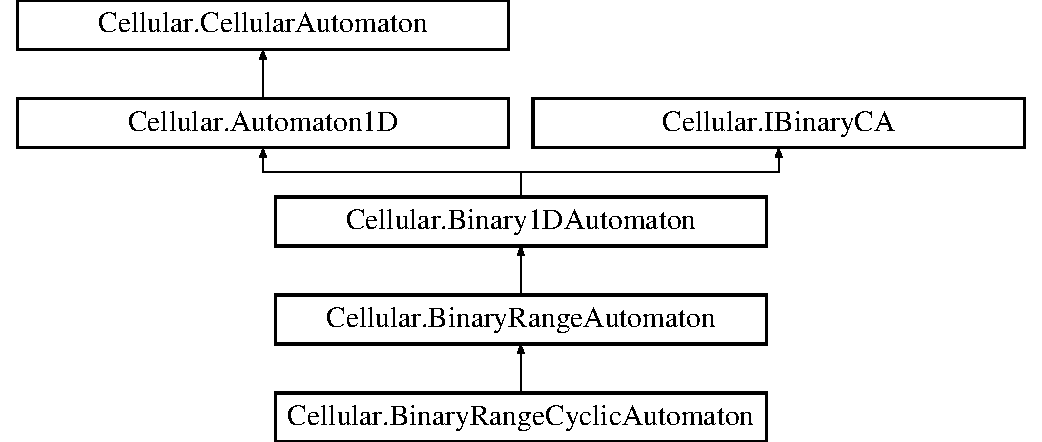
\includegraphics[height=5.000000cm]{class_cellular_1_1_binary_range_cyclic_automaton}
\end{center}
\end{figure}
\subsection*{Public Member Functions}
\begin{DoxyCompactItemize}
\item 
\hyperlink{class_cellular_1_1_binary_range_cyclic_automaton_a9f47b4027eba7db4a959946967ba371e}{Binary\+Range\+Cyclic\+Automaton} (byte scope, bool\mbox{[}$\,$\mbox{]} \hyperlink{class_cellular_1_1_binary_range_automaton_a4dda99c3151599c8ef12d08d7472144c}{rule}, int \hyperlink{class_cellular_1_1_automaton1_d_a915129ccf0f1e7092844c99ce6a28e5b}{size})
\begin{DoxyCompactList}\small\item\em Creates a new cyclic C\+A of a general rule with 000...00100...000 as its initial state. \end{DoxyCompactList}\item 
\hyperlink{class_cellular_1_1_binary_range_cyclic_automaton_a541a8c6eff23ec8afddc7388158df80e}{Binary\+Range\+Cyclic\+Automaton} (byte scope, bool\mbox{[}$\,$\mbox{]} \hyperlink{class_cellular_1_1_binary_range_automaton_a4dda99c3151599c8ef12d08d7472144c}{rule}, Bit\+Array \hyperlink{all__1_8js_ae8b87ff4be2ae1dd5267342795263360}{initial\+State})
\begin{DoxyCompactList}\small\item\em Creates a new cyclic C\+A of a general rule with defined inital state. \end{DoxyCompactList}\item 
override object \hyperlink{class_cellular_1_1_binary_range_cyclic_automaton_a2361fe82802e372b24b8bec6a6135278}{Clone} ()
\begin{DoxyCompactList}\small\item\em Creates an appropriate copy of the C\+A. Its type and the specific rule are always preserved. However, the time (number of steps executed on the specific instance) is set back to 0. \end{DoxyCompactList}\item 
override string \hyperlink{class_cellular_1_1_binary_range_cyclic_automaton_a75754d1c54550e1f29a9282647947cb8}{Tell\+Type} ()
\begin{DoxyCompactList}\small\item\em Announces the runtime type of the C\+A including info about its rule. It serves for debugging purposes. \end{DoxyCompactList}\item 
\hyperlink{class_cellular_1_1_reversible_automaton}{Reversible\+Automaton} \hyperlink{class_cellular_1_1_binary_range_cyclic_automaton_a68dc88c2cb78aaaf6246ebf6f058fbb9}{Convert\+To\+Reversible} (Bit\+Array previous\+State)
\end{DoxyCompactItemize}
\subsection*{Protected Member Functions}
\begin{DoxyCompactItemize}
\item 
override bool \hyperlink{class_cellular_1_1_binary_range_cyclic_automaton_a0e4d7dd11fda253300ee9fc8adbc4d33}{get\+Value\+At} (int index)
\begin{DoxyCompactList}\small\item\em This method simplifies boundary conditions. \end{DoxyCompactList}\item 
override \hyperlink{interface_cellular_1_1_i_binary_c_a}{I\+Binary\+C\+A} \hyperlink{class_cellular_1_1_binary_range_cyclic_automaton_a38ebc4d1f2610701299106475229c60b}{clone\+Template} (Bit\+Array new\+Instance\+State)
\end{DoxyCompactItemize}
\subsection*{Additional Inherited Members}


\subsection{Detailed Description}
Class representing any binary 1\+D automaton with symmetric scope. The automaton is cyclic -\/ its edges are connected. Therefore, all positions are equivalent. 



Definition at line 9 of file Binary\+Range\+Cyclic\+Automaton.\+cs.



\subsection{Constructor \& Destructor Documentation}
\hypertarget{class_cellular_1_1_binary_range_cyclic_automaton_a9f47b4027eba7db4a959946967ba371e}{}\index{Cellular\+::\+Binary\+Range\+Cyclic\+Automaton@{Cellular\+::\+Binary\+Range\+Cyclic\+Automaton}!Binary\+Range\+Cyclic\+Automaton@{Binary\+Range\+Cyclic\+Automaton}}
\index{Binary\+Range\+Cyclic\+Automaton@{Binary\+Range\+Cyclic\+Automaton}!Cellular\+::\+Binary\+Range\+Cyclic\+Automaton@{Cellular\+::\+Binary\+Range\+Cyclic\+Automaton}}
\subsubsection[{Binary\+Range\+Cyclic\+Automaton(byte scope, bool[] rule, int size)}]{\setlength{\rightskip}{0pt plus 5cm}Cellular.\+Binary\+Range\+Cyclic\+Automaton.\+Binary\+Range\+Cyclic\+Automaton (
\begin{DoxyParamCaption}
\item[{byte}]{scope, }
\item[{bool\mbox{[}$\,$\mbox{]}}]{rule, }
\item[{int}]{size}
\end{DoxyParamCaption}
)}\label{class_cellular_1_1_binary_range_cyclic_automaton_a9f47b4027eba7db4a959946967ba371e}


Creates a new cyclic C\+A of a general rule with 000...00100...000 as its initial state. 


\begin{DoxyParams}{Parameters}
{\em scope} & How many cells on each side from the center determine the next state of the cell. Value 1 makes it equivalent to a {\ttfamily \hyperlink{class_cellular_1_1_elementary_automaton}{Elementary\+Automaton}} which has rule of size 8. Value 2 means that each new state of any cell depends on five total cells =$>$ size of rule must be 32.\\
\hline
{\em rule} & Array representing the rule for creating a new state. rule\mbox{[}0\mbox{]} is rule for 0..0, therefore opposite order to the rules of basic automata.\\
\hline
{\em size} & The size of the new C\+A.\\
\hline
\end{DoxyParams}


Definition at line 20 of file Binary\+Range\+Cyclic\+Automaton.\+cs.

\hypertarget{class_cellular_1_1_binary_range_cyclic_automaton_a541a8c6eff23ec8afddc7388158df80e}{}\index{Cellular\+::\+Binary\+Range\+Cyclic\+Automaton@{Cellular\+::\+Binary\+Range\+Cyclic\+Automaton}!Binary\+Range\+Cyclic\+Automaton@{Binary\+Range\+Cyclic\+Automaton}}
\index{Binary\+Range\+Cyclic\+Automaton@{Binary\+Range\+Cyclic\+Automaton}!Cellular\+::\+Binary\+Range\+Cyclic\+Automaton@{Cellular\+::\+Binary\+Range\+Cyclic\+Automaton}}
\subsubsection[{Binary\+Range\+Cyclic\+Automaton(byte scope, bool[] rule, Bit\+Array initial\+State)}]{\setlength{\rightskip}{0pt plus 5cm}Cellular.\+Binary\+Range\+Cyclic\+Automaton.\+Binary\+Range\+Cyclic\+Automaton (
\begin{DoxyParamCaption}
\item[{byte}]{scope, }
\item[{bool\mbox{[}$\,$\mbox{]}}]{rule, }
\item[{Bit\+Array}]{initial\+State}
\end{DoxyParamCaption}
)}\label{class_cellular_1_1_binary_range_cyclic_automaton_a541a8c6eff23ec8afddc7388158df80e}


Creates a new cyclic C\+A of a general rule with defined inital state. 


\begin{DoxyParams}{Parameters}
{\em scope} & How many cells on each side from the center determine the next state of the cell. Value 1 makes it equivalent to a {\ttfamily \hyperlink{class_cellular_1_1_elementary_automaton}{Elementary\+Automaton}} which has rule of size 8. Value 2 means that each new state of any cell depends on five total cells =$>$ size of rule must be 32.\\
\hline
{\em rule} & Array representing the rule for creating a new state. rule\mbox{[}0\mbox{]} is rule for 0..0, therefore opposite order to the rules of basic automata.\\
\hline
{\em initial\+State} & A {\ttfamily Bit\+Array} describing the initial state of the C\+A. This also determines the size of the new C\+A.\\
\hline
\end{DoxyParams}


Definition at line 32 of file Binary\+Range\+Cyclic\+Automaton.\+cs.



\subsection{Member Function Documentation}
\hypertarget{class_cellular_1_1_binary_range_cyclic_automaton_a2361fe82802e372b24b8bec6a6135278}{}\index{Cellular\+::\+Binary\+Range\+Cyclic\+Automaton@{Cellular\+::\+Binary\+Range\+Cyclic\+Automaton}!Clone@{Clone}}
\index{Clone@{Clone}!Cellular\+::\+Binary\+Range\+Cyclic\+Automaton@{Cellular\+::\+Binary\+Range\+Cyclic\+Automaton}}
\subsubsection[{Clone()}]{\setlength{\rightskip}{0pt plus 5cm}override object Cellular.\+Binary\+Range\+Cyclic\+Automaton.\+Clone (
\begin{DoxyParamCaption}
{}
\end{DoxyParamCaption}
)\hspace{0.3cm}{\ttfamily [virtual]}}\label{class_cellular_1_1_binary_range_cyclic_automaton_a2361fe82802e372b24b8bec6a6135278}


Creates an appropriate copy of the C\+A. Its type and the specific rule are always preserved. However, the time (number of steps executed on the specific instance) is set back to 0. 

\begin{DoxyReturn}{Returns}
A copy of the {\ttfamily \hyperlink{class_cellular_1_1_cellular_automaton}{Cellular\+Automaton}} as an {\ttfamily Object}
\end{DoxyReturn}


Reimplemented from \hyperlink{class_cellular_1_1_binary_range_automaton_a12f010562e04785e0a7efb113302687e}{Cellular.\+Binary\+Range\+Automaton}.



Definition at line 46 of file Binary\+Range\+Cyclic\+Automaton.\+cs.

\hypertarget{class_cellular_1_1_binary_range_cyclic_automaton_a38ebc4d1f2610701299106475229c60b}{}\index{Cellular\+::\+Binary\+Range\+Cyclic\+Automaton@{Cellular\+::\+Binary\+Range\+Cyclic\+Automaton}!clone\+Template@{clone\+Template}}
\index{clone\+Template@{clone\+Template}!Cellular\+::\+Binary\+Range\+Cyclic\+Automaton@{Cellular\+::\+Binary\+Range\+Cyclic\+Automaton}}
\subsubsection[{clone\+Template(\+Bit\+Array new\+Instance\+State)}]{\setlength{\rightskip}{0pt plus 5cm}override {\bf I\+Binary\+C\+A} Cellular.\+Binary\+Range\+Cyclic\+Automaton.\+clone\+Template (
\begin{DoxyParamCaption}
\item[{Bit\+Array}]{new\+Instance\+State}
\end{DoxyParamCaption}
)\hspace{0.3cm}{\ttfamily [protected]}, {\ttfamily [virtual]}}\label{class_cellular_1_1_binary_range_cyclic_automaton_a38ebc4d1f2610701299106475229c60b}


Reimplemented from \hyperlink{class_cellular_1_1_binary_range_automaton_a75d9e1fc19f9bfc470e66b12aaf1abe8}{Cellular.\+Binary\+Range\+Automaton}.



Definition at line 51 of file Binary\+Range\+Cyclic\+Automaton.\+cs.

\hypertarget{class_cellular_1_1_binary_range_cyclic_automaton_a68dc88c2cb78aaaf6246ebf6f058fbb9}{}\index{Cellular\+::\+Binary\+Range\+Cyclic\+Automaton@{Cellular\+::\+Binary\+Range\+Cyclic\+Automaton}!Convert\+To\+Reversible@{Convert\+To\+Reversible}}
\index{Convert\+To\+Reversible@{Convert\+To\+Reversible}!Cellular\+::\+Binary\+Range\+Cyclic\+Automaton@{Cellular\+::\+Binary\+Range\+Cyclic\+Automaton}}
\subsubsection[{Convert\+To\+Reversible(\+Bit\+Array previous\+State)}]{\setlength{\rightskip}{0pt plus 5cm}{\bf Reversible\+Automaton} Cellular.\+Binary\+Range\+Cyclic\+Automaton.\+Convert\+To\+Reversible (
\begin{DoxyParamCaption}
\item[{Bit\+Array}]{previous\+State}
\end{DoxyParamCaption}
)}\label{class_cellular_1_1_binary_range_cyclic_automaton_a68dc88c2cb78aaaf6246ebf6f058fbb9}


Definition at line 61 of file Binary\+Range\+Cyclic\+Automaton.\+cs.

\hypertarget{class_cellular_1_1_binary_range_cyclic_automaton_a0e4d7dd11fda253300ee9fc8adbc4d33}{}\index{Cellular\+::\+Binary\+Range\+Cyclic\+Automaton@{Cellular\+::\+Binary\+Range\+Cyclic\+Automaton}!get\+Value\+At@{get\+Value\+At}}
\index{get\+Value\+At@{get\+Value\+At}!Cellular\+::\+Binary\+Range\+Cyclic\+Automaton@{Cellular\+::\+Binary\+Range\+Cyclic\+Automaton}}
\subsubsection[{get\+Value\+At(int index)}]{\setlength{\rightskip}{0pt plus 5cm}override bool Cellular.\+Binary\+Range\+Cyclic\+Automaton.\+get\+Value\+At (
\begin{DoxyParamCaption}
\item[{int}]{index}
\end{DoxyParamCaption}
)\hspace{0.3cm}{\ttfamily [protected]}, {\ttfamily [virtual]}}\label{class_cellular_1_1_binary_range_cyclic_automaton_a0e4d7dd11fda253300ee9fc8adbc4d33}


This method simplifies boundary conditions. 


\begin{DoxyParams}{Parameters}
{\em index} & Zero-\/based index (which bit is required).\\
\hline
\end{DoxyParams}
\begin{DoxyReturn}{Returns}
One bit.
\end{DoxyReturn}


Reimplemented from \hyperlink{class_cellular_1_1_binary_range_automaton_a462f8b1d9b77966e14bb0160a4a06dca}{Cellular.\+Binary\+Range\+Automaton}.



Definition at line 34 of file Binary\+Range\+Cyclic\+Automaton.\+cs.

\hypertarget{class_cellular_1_1_binary_range_cyclic_automaton_a75754d1c54550e1f29a9282647947cb8}{}\index{Cellular\+::\+Binary\+Range\+Cyclic\+Automaton@{Cellular\+::\+Binary\+Range\+Cyclic\+Automaton}!Tell\+Type@{Tell\+Type}}
\index{Tell\+Type@{Tell\+Type}!Cellular\+::\+Binary\+Range\+Cyclic\+Automaton@{Cellular\+::\+Binary\+Range\+Cyclic\+Automaton}}
\subsubsection[{Tell\+Type()}]{\setlength{\rightskip}{0pt plus 5cm}override string Cellular.\+Binary\+Range\+Cyclic\+Automaton.\+Tell\+Type (
\begin{DoxyParamCaption}
{}
\end{DoxyParamCaption}
)}\label{class_cellular_1_1_binary_range_cyclic_automaton_a75754d1c54550e1f29a9282647947cb8}


Announces the runtime type of the C\+A including info about its rule. It serves for debugging purposes. 

\begin{DoxyReturn}{Returns}
The same string as calling {\ttfamily \hyperlink{class_cellular_1_1_cellular_automaton_abe4b92fd405530c8a08cc07a3a19fff4}{Cellular\+Automaton.\+Tell\+Type()}}.
\end{DoxyReturn}


Implements \hyperlink{interface_cellular_1_1_i_binary_c_a_aa67feabf5d1513aa74076d255c661948}{Cellular.\+I\+Binary\+C\+A}.



Definition at line 56 of file Binary\+Range\+Cyclic\+Automaton.\+cs.



The documentation for this class was generated from the following file\+:\begin{DoxyCompactItemize}
\item 
C\+:/\+Martin/\+M\+F\+F/\+\_\+baka/\+Martin\+Dvorak/\+Cellular/\hyperlink{_binary_range_cyclic_automaton_8cs}{Binary\+Range\+Cyclic\+Automaton.\+cs}\end{DoxyCompactItemize}

\hypertarget{class_testing_1_1_binary_range_n_test}{}\section{Testing.\+Binary\+Range\+N\+Test Class Reference}
\label{class_testing_1_1_binary_range_n_test}\index{Testing.\+Binary\+Range\+N\+Test@{Testing.\+Binary\+Range\+N\+Test}}


Simple demonstration that {\ttfamily Binary\+Range\+Automaton} can be used in a place of {\ttfamily Elementary\+Automaton}.  


\subsection*{Static Public Member Functions}
\begin{DoxyCompactItemize}
\item 
static void \hyperlink{class_testing_1_1_binary_range_n_test_aa53181f8247ace374a9d9d291ba2170d}{Run\+Test} ()
\end{DoxyCompactItemize}


\subsection{Detailed Description}
Simple demonstration that {\ttfamily Binary\+Range\+Automaton} can be used in a place of {\ttfamily Elementary\+Automaton}. 



Definition at line 9 of file Binary\+Range\+N\+Test.\+cs.



\subsection{Member Function Documentation}
\hypertarget{class_testing_1_1_binary_range_n_test_aa53181f8247ace374a9d9d291ba2170d}{}\index{Testing\+::\+Binary\+Range\+N\+Test@{Testing\+::\+Binary\+Range\+N\+Test}!Run\+Test@{Run\+Test}}
\index{Run\+Test@{Run\+Test}!Testing\+::\+Binary\+Range\+N\+Test@{Testing\+::\+Binary\+Range\+N\+Test}}
\subsubsection[{Run\+Test()}]{\setlength{\rightskip}{0pt plus 5cm}static void Testing.\+Binary\+Range\+N\+Test.\+Run\+Test (
\begin{DoxyParamCaption}
{}
\end{DoxyParamCaption}
)\hspace{0.3cm}{\ttfamily [static]}}\label{class_testing_1_1_binary_range_n_test_aa53181f8247ace374a9d9d291ba2170d}


Definition at line 11 of file Binary\+Range\+N\+Test.\+cs.



The documentation for this class was generated from the following file\+:\begin{DoxyCompactItemize}
\item 
C\+:/\+Martin/\+M\+F\+F/\+\_\+baka/\+Martin\+Dvorak/\+Testing/\hyperlink{_binary_range_n_test_8cs}{Binary\+Range\+N\+Test.\+cs}\end{DoxyCompactItemize}

\hypertarget{class_crypto_1_1_cannot_generate_exception}{}\section{Crypto.\+Cannot\+Generate\+Exception Class Reference}
\label{class_crypto_1_1_cannot_generate_exception}\index{Crypto.\+Cannot\+Generate\+Exception@{Crypto.\+Cannot\+Generate\+Exception}}


Custom exception that any key extender can throw.  


Inheritance diagram for Crypto.\+Cannot\+Generate\+Exception\+:\begin{figure}[H]
\begin{center}
\leavevmode
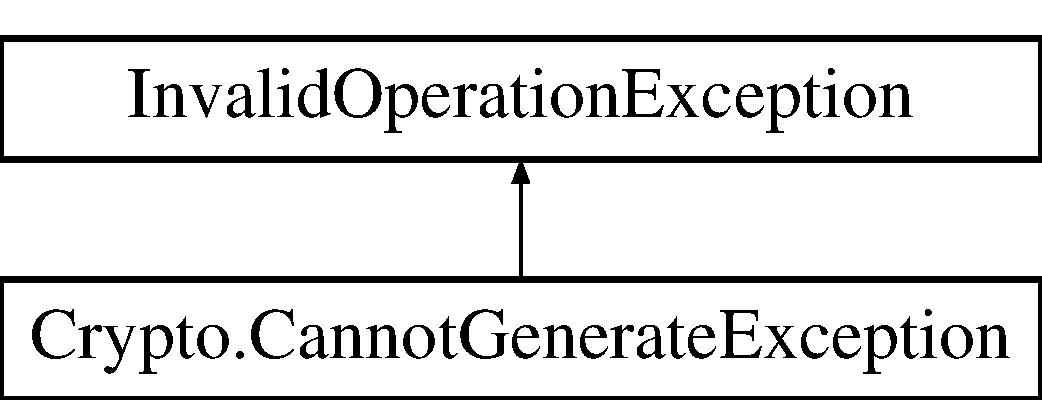
\includegraphics[height=2.000000cm]{class_crypto_1_1_cannot_generate_exception}
\end{center}
\end{figure}
\subsection*{Public Member Functions}
\begin{DoxyCompactItemize}
\item 
\hyperlink{class_crypto_1_1_cannot_generate_exception_a17a4ab8ac6a435318f69bf88ae224598}{Cannot\+Generate\+Exception} ()
\item 
\hyperlink{class_crypto_1_1_cannot_generate_exception_acc186360edfaaa431c4c64ef7562dd56}{Cannot\+Generate\+Exception} (string message)
\item 
\hyperlink{class_crypto_1_1_cannot_generate_exception_a85fc7abc1f61642c128e1d14d2985ecf}{Cannot\+Generate\+Exception} (string message, Exception inner\+Exception)
\end{DoxyCompactItemize}


\subsection{Detailed Description}
Custom exception that any key extender can throw. 



Definition at line 8 of file Cannot\+Generate\+Exception.\+cs.



\subsection{Constructor \& Destructor Documentation}
\hypertarget{class_crypto_1_1_cannot_generate_exception_a17a4ab8ac6a435318f69bf88ae224598}{}\index{Crypto\+::\+Cannot\+Generate\+Exception@{Crypto\+::\+Cannot\+Generate\+Exception}!Cannot\+Generate\+Exception@{Cannot\+Generate\+Exception}}
\index{Cannot\+Generate\+Exception@{Cannot\+Generate\+Exception}!Crypto\+::\+Cannot\+Generate\+Exception@{Crypto\+::\+Cannot\+Generate\+Exception}}
\subsubsection[{Cannot\+Generate\+Exception()}]{\setlength{\rightskip}{0pt plus 5cm}Crypto.\+Cannot\+Generate\+Exception.\+Cannot\+Generate\+Exception (
\begin{DoxyParamCaption}
{}
\end{DoxyParamCaption}
)}\label{class_crypto_1_1_cannot_generate_exception_a17a4ab8ac6a435318f69bf88ae224598}


Definition at line 10 of file Cannot\+Generate\+Exception.\+cs.

\hypertarget{class_crypto_1_1_cannot_generate_exception_acc186360edfaaa431c4c64ef7562dd56}{}\index{Crypto\+::\+Cannot\+Generate\+Exception@{Crypto\+::\+Cannot\+Generate\+Exception}!Cannot\+Generate\+Exception@{Cannot\+Generate\+Exception}}
\index{Cannot\+Generate\+Exception@{Cannot\+Generate\+Exception}!Crypto\+::\+Cannot\+Generate\+Exception@{Crypto\+::\+Cannot\+Generate\+Exception}}
\subsubsection[{Cannot\+Generate\+Exception(string message)}]{\setlength{\rightskip}{0pt plus 5cm}Crypto.\+Cannot\+Generate\+Exception.\+Cannot\+Generate\+Exception (
\begin{DoxyParamCaption}
\item[{string}]{message}
\end{DoxyParamCaption}
)}\label{class_crypto_1_1_cannot_generate_exception_acc186360edfaaa431c4c64ef7562dd56}


Definition at line 11 of file Cannot\+Generate\+Exception.\+cs.

\hypertarget{class_crypto_1_1_cannot_generate_exception_a85fc7abc1f61642c128e1d14d2985ecf}{}\index{Crypto\+::\+Cannot\+Generate\+Exception@{Crypto\+::\+Cannot\+Generate\+Exception}!Cannot\+Generate\+Exception@{Cannot\+Generate\+Exception}}
\index{Cannot\+Generate\+Exception@{Cannot\+Generate\+Exception}!Crypto\+::\+Cannot\+Generate\+Exception@{Crypto\+::\+Cannot\+Generate\+Exception}}
\subsubsection[{Cannot\+Generate\+Exception(string message, Exception inner\+Exception)}]{\setlength{\rightskip}{0pt plus 5cm}Crypto.\+Cannot\+Generate\+Exception.\+Cannot\+Generate\+Exception (
\begin{DoxyParamCaption}
\item[{string}]{message, }
\item[{Exception}]{inner\+Exception}
\end{DoxyParamCaption}
)}\label{class_crypto_1_1_cannot_generate_exception_a85fc7abc1f61642c128e1d14d2985ecf}


Definition at line 12 of file Cannot\+Generate\+Exception.\+cs.



The documentation for this class was generated from the following file\+:\begin{DoxyCompactItemize}
\item 
C\+:/\+Martin/\+M\+F\+F/\+\_\+baka/\+Martin\+Dvorak/\+Crypto/\hyperlink{_cannot_generate_exception_8cs}{Cannot\+Generate\+Exception.\+cs}\end{DoxyCompactItemize}

\hypertarget{class_cellular_1_1_cellular_automaton}{}\section{Cellular.\+Cellular\+Automaton Class Reference}
\label{class_cellular_1_1_cellular_automaton}\index{Cellular.\+Cellular\+Automaton@{Cellular.\+Cellular\+Automaton}}


The top class of the C\+A hierarchy. Every constructor should follow this logical order when considering its parametres\+: specification of the type (usually not needed), rule, size, initial state / rng.  


Inheritance diagram for Cellular.\+Cellular\+Automaton\+:\begin{figure}[H]
\begin{center}
\leavevmode
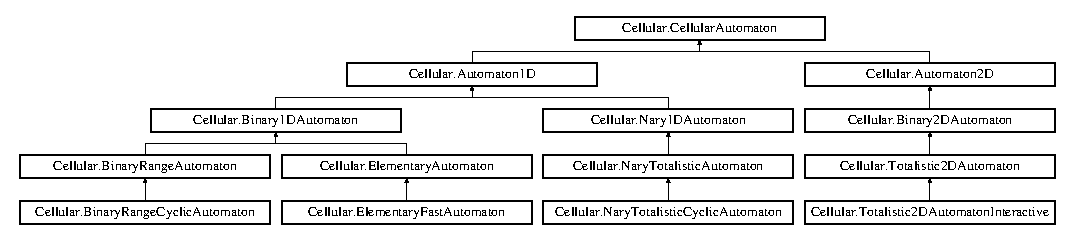
\includegraphics[height=2.231076cm]{class_cellular_1_1_cellular_automaton}
\end{center}
\end{figure}
\subsection*{Public Member Functions}
\begin{DoxyCompactItemize}
\item 
abstract void \hyperlink{class_cellular_1_1_cellular_automaton_aa70848d58015575974bc875ac5a89ae7}{Step} ()
\begin{DoxyCompactList}\small\item\em Performs one step applying the specific rule for creating a new state. \end{DoxyCompactList}\item 
uint \hyperlink{class_cellular_1_1_cellular_automaton_a340d1faea1300db9183b4b4368d4f838}{Get\+Time} ()
\begin{DoxyCompactList}\small\item\em Only returns how many steps have been done. \end{DoxyCompactList}\item 
void \hyperlink{class_cellular_1_1_cellular_automaton_ad4948be8db73c5e052e2c5e59ac85ad8}{Step} (uint times)
\begin{DoxyCompactList}\small\item\em Performs the step n times. \end{DoxyCompactList}\item 
abstract object \hyperlink{class_cellular_1_1_cellular_automaton_affd487b397cdbbbb1982815bbcd8e7d3}{Clone} ()
\begin{DoxyCompactList}\small\item\em Creates an appropriate copy of the C\+A. Its type and the specific rule are always preserved. However, the time (number of steps executed on the specific instance) is set back to 0. \end{DoxyCompactList}\item 
abstract string \hyperlink{class_cellular_1_1_cellular_automaton_abe4b92fd405530c8a08cc07a3a19fff4}{Tell\+Type} ()
\begin{DoxyCompactList}\small\item\em Announces the runtime type of the C\+A including info about its rule. It serves for debugging purposes. \end{DoxyCompactList}\end{DoxyCompactItemize}
\subsection*{Protected Attributes}
\begin{DoxyCompactItemize}
\item 
uint \hyperlink{class_cellular_1_1_cellular_automaton_a6eaa8a9840fbc4c875d4e7d5a14e5f70}{time} = 0
\end{DoxyCompactItemize}


\subsection{Detailed Description}
The top class of the C\+A hierarchy. Every constructor should follow this logical order when considering its parametres\+: specification of the type (usually not needed), rule, size, initial state / rng. 



Definition at line 7 of file Cellular\+Automaton.\+cs.



\subsection{Member Function Documentation}
\hypertarget{class_cellular_1_1_cellular_automaton_affd487b397cdbbbb1982815bbcd8e7d3}{}\index{Cellular\+::\+Cellular\+Automaton@{Cellular\+::\+Cellular\+Automaton}!Clone@{Clone}}
\index{Clone@{Clone}!Cellular\+::\+Cellular\+Automaton@{Cellular\+::\+Cellular\+Automaton}}
\subsubsection[{Clone()}]{\setlength{\rightskip}{0pt plus 5cm}abstract object Cellular.\+Cellular\+Automaton.\+Clone (
\begin{DoxyParamCaption}
{}
\end{DoxyParamCaption}
)\hspace{0.3cm}{\ttfamily [pure virtual]}}\label{class_cellular_1_1_cellular_automaton_affd487b397cdbbbb1982815bbcd8e7d3}


Creates an appropriate copy of the C\+A. Its type and the specific rule are always preserved. However, the time (number of steps executed on the specific instance) is set back to 0. 

\begin{DoxyReturn}{Returns}
A copy of the {\ttfamily \hyperlink{class_cellular_1_1_cellular_automaton}{Cellular\+Automaton}} as an {\ttfamily Object}
\end{DoxyReturn}


Implemented in \hyperlink{class_cellular_1_1_totalistic2_d_automaton_ae78cf4c3f8245adf64ec9a173330804f}{Cellular.\+Totalistic2\+D\+Automaton}, \hyperlink{class_cellular_1_1_elementary_fast_automaton_a98bbdcade0ac93dd0fbc96ba253c2978}{Cellular.\+Elementary\+Fast\+Automaton}, \hyperlink{class_cellular_1_1_binary_range_automaton_a12f010562e04785e0a7efb113302687e}{Cellular.\+Binary\+Range\+Automaton}, \hyperlink{class_cellular_1_1_elementary_automaton_ada4ddee98167e8f4f4b6dea1f7563b47}{Cellular.\+Elementary\+Automaton}, \hyperlink{class_cellular_1_1_reversible_automaton_a276aa112cccc2513c6b7c005056205fb}{Cellular.\+Reversible\+Automaton}, \hyperlink{class_cellular_1_1_binary_range_cyclic_automaton_a2361fe82802e372b24b8bec6a6135278}{Cellular.\+Binary\+Range\+Cyclic\+Automaton}, \hyperlink{class_cellular_1_1_nary_totalistic_automaton_a13f16113915ecec451fc4764a32044f9}{Cellular.\+Nary\+Totalistic\+Automaton}, and \hyperlink{class_cellular_1_1_nary_totalistic_cyclic_automaton_aa8d5a7d77a6dfc5f6e4fae6ba1c6cfd0}{Cellular.\+Nary\+Totalistic\+Cyclic\+Automaton}.

\hypertarget{class_cellular_1_1_cellular_automaton_a340d1faea1300db9183b4b4368d4f838}{}\index{Cellular\+::\+Cellular\+Automaton@{Cellular\+::\+Cellular\+Automaton}!Get\+Time@{Get\+Time}}
\index{Get\+Time@{Get\+Time}!Cellular\+::\+Cellular\+Automaton@{Cellular\+::\+Cellular\+Automaton}}
\subsubsection[{Get\+Time()}]{\setlength{\rightskip}{0pt plus 5cm}uint Cellular.\+Cellular\+Automaton.\+Get\+Time (
\begin{DoxyParamCaption}
{}
\end{DoxyParamCaption}
)}\label{class_cellular_1_1_cellular_automaton_a340d1faea1300db9183b4b4368d4f838}


Only returns how many steps have been done. 

\begin{DoxyReturn}{Returns}
Number of executed steps.
\end{DoxyReturn}


Definition at line 20 of file Cellular\+Automaton.\+cs.

\hypertarget{class_cellular_1_1_cellular_automaton_aa70848d58015575974bc875ac5a89ae7}{}\index{Cellular\+::\+Cellular\+Automaton@{Cellular\+::\+Cellular\+Automaton}!Step@{Step}}
\index{Step@{Step}!Cellular\+::\+Cellular\+Automaton@{Cellular\+::\+Cellular\+Automaton}}
\subsubsection[{Step()}]{\setlength{\rightskip}{0pt plus 5cm}abstract void Cellular.\+Cellular\+Automaton.\+Step (
\begin{DoxyParamCaption}
{}
\end{DoxyParamCaption}
)\hspace{0.3cm}{\ttfamily [pure virtual]}}\label{class_cellular_1_1_cellular_automaton_aa70848d58015575974bc875ac5a89ae7}


Performs one step applying the specific rule for creating a new state. 



Implemented in \hyperlink{class_cellular_1_1_totalistic2_d_automaton_a7f85cac5420f67a936cbd4cef33c4abc}{Cellular.\+Totalistic2\+D\+Automaton}, \hyperlink{class_cellular_1_1_elementary_automaton_adae7c322e4c7cd00cd0534a23d1abfa4}{Cellular.\+Elementary\+Automaton}, \hyperlink{class_cellular_1_1_binary_range_automaton_ade1f5b831b9676f04f835c33d245b9e2}{Cellular.\+Binary\+Range\+Automaton}, \hyperlink{class_cellular_1_1_elementary_fast_automaton_aa877bef8b8242c58e190a884d18f3b5f}{Cellular.\+Elementary\+Fast\+Automaton}, \hyperlink{class_cellular_1_1_reversible_automaton_ae931cb64ab215ba1d1c1019a3f289b6d}{Cellular.\+Reversible\+Automaton}, and \hyperlink{class_cellular_1_1_nary_totalistic_automaton_ad90769a438ab94b46d4750a571782056}{Cellular.\+Nary\+Totalistic\+Automaton}.

\hypertarget{class_cellular_1_1_cellular_automaton_ad4948be8db73c5e052e2c5e59ac85ad8}{}\index{Cellular\+::\+Cellular\+Automaton@{Cellular\+::\+Cellular\+Automaton}!Step@{Step}}
\index{Step@{Step}!Cellular\+::\+Cellular\+Automaton@{Cellular\+::\+Cellular\+Automaton}}
\subsubsection[{Step(uint times)}]{\setlength{\rightskip}{0pt plus 5cm}void Cellular.\+Cellular\+Automaton.\+Step (
\begin{DoxyParamCaption}
\item[{uint}]{times}
\end{DoxyParamCaption}
)}\label{class_cellular_1_1_cellular_automaton_ad4948be8db73c5e052e2c5e59ac85ad8}


Performs the step n times. 


\begin{DoxyParams}{Parameters}
{\em times} & How many times {\ttfamily \hyperlink{class_cellular_1_1_cellular_automaton_aa70848d58015575974bc875ac5a89ae7}{Step()}} should be called.\\
\hline
\end{DoxyParams}


Definition at line 29 of file Cellular\+Automaton.\+cs.

\hypertarget{class_cellular_1_1_cellular_automaton_abe4b92fd405530c8a08cc07a3a19fff4}{}\index{Cellular\+::\+Cellular\+Automaton@{Cellular\+::\+Cellular\+Automaton}!Tell\+Type@{Tell\+Type}}
\index{Tell\+Type@{Tell\+Type}!Cellular\+::\+Cellular\+Automaton@{Cellular\+::\+Cellular\+Automaton}}
\subsubsection[{Tell\+Type()}]{\setlength{\rightskip}{0pt plus 5cm}abstract string Cellular.\+Cellular\+Automaton.\+Tell\+Type (
\begin{DoxyParamCaption}
{}
\end{DoxyParamCaption}
)\hspace{0.3cm}{\ttfamily [pure virtual]}}\label{class_cellular_1_1_cellular_automaton_abe4b92fd405530c8a08cc07a3a19fff4}


Announces the runtime type of the C\+A including info about its rule. It serves for debugging purposes. 

\begin{DoxyReturn}{Returns}
Type of the C\+A as a string.
\end{DoxyReturn}


Implemented in \hyperlink{class_cellular_1_1_totalistic2_d_automaton_aa009c674cd109fa70173e9893f6d3b09}{Cellular.\+Totalistic2\+D\+Automaton}, \hyperlink{class_cellular_1_1_binary_range_automaton_afad205eb4fea51efd63b063f96bfda5c}{Cellular.\+Binary\+Range\+Automaton}, \hyperlink{class_cellular_1_1_elementary_automaton_a812677139d560e2c600226361b785995}{Cellular.\+Elementary\+Automaton}, \hyperlink{class_cellular_1_1_reversible_automaton_ae394a104b5fe5a550c6c378fea92c355}{Cellular.\+Reversible\+Automaton}, \hyperlink{class_cellular_1_1_binary_range_cyclic_automaton_a75754d1c54550e1f29a9282647947cb8}{Cellular.\+Binary\+Range\+Cyclic\+Automaton}, \hyperlink{class_cellular_1_1_nary_totalistic_automaton_aa691c532a55638c7e3d0c125a4244773}{Cellular.\+Nary\+Totalistic\+Automaton}, and \hyperlink{class_cellular_1_1_nary_totalistic_cyclic_automaton_ac5c39cfb72386e3ab6132ab420091ae9}{Cellular.\+Nary\+Totalistic\+Cyclic\+Automaton}.



\subsection{Member Data Documentation}
\hypertarget{class_cellular_1_1_cellular_automaton_a6eaa8a9840fbc4c875d4e7d5a14e5f70}{}\index{Cellular\+::\+Cellular\+Automaton@{Cellular\+::\+Cellular\+Automaton}!time@{time}}
\index{time@{time}!Cellular\+::\+Cellular\+Automaton@{Cellular\+::\+Cellular\+Automaton}}
\subsubsection[{time}]{\setlength{\rightskip}{0pt plus 5cm}uint Cellular.\+Cellular\+Automaton.\+time = 0\hspace{0.3cm}{\ttfamily [protected]}}\label{class_cellular_1_1_cellular_automaton_a6eaa8a9840fbc4c875d4e7d5a14e5f70}


Definition at line 9 of file Cellular\+Automaton.\+cs.



The documentation for this class was generated from the following file\+:\begin{DoxyCompactItemize}
\item 
C\+:/\+Martin/\+M\+F\+F/\+\_\+baka/\+Martin\+Dvorak/\+Cellular/\hyperlink{_cellular_automaton_8cs}{Cellular\+Automaton.\+cs}\end{DoxyCompactItemize}

\input{class_cryptography_unit_tests_1_1_common_part}
\hypertarget{class_program_1_1_crypto_form}{}\section{Program.\+Crypto\+Form Class Reference}
\label{class_program_1_1_crypto_form}\index{Program.\+Crypto\+Form@{Program.\+Crypto\+Form}}


Windows application for users who want to encrypt their data using a cellular automata based algorithm.  


Inheritance diagram for Program.\+Crypto\+Form\+:\begin{figure}[H]
\begin{center}
\leavevmode
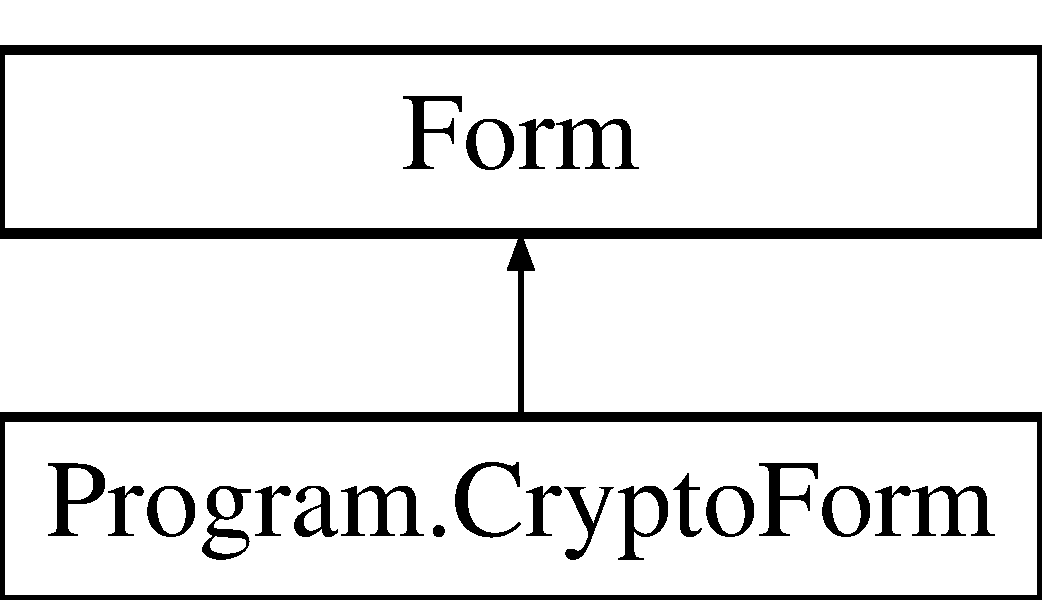
\includegraphics[height=2.000000cm]{class_program_1_1_crypto_form}
\end{center}
\end{figure}
\subsection*{Public Member Functions}
\begin{DoxyCompactItemize}
\item 
\hyperlink{class_program_1_1_crypto_form_ab4de171d2fe2499055864e45f9efa4cc}{Crypto\+Form} ()
\end{DoxyCompactItemize}
\subsection*{Protected Member Functions}
\begin{DoxyCompactItemize}
\item 
override void \hyperlink{class_program_1_1_crypto_form_adaa80d92f4324b9d835d8125dcda4582}{Dispose} (bool disposing)
\begin{DoxyCompactList}\small\item\em Clean up any resources being used. \end{DoxyCompactList}\end{DoxyCompactItemize}


\subsection{Detailed Description}
Windows application for users who want to encrypt their data using a cellular automata based algorithm. 



Definition at line 14 of file Crypto\+Form.\+cs.



\subsection{Constructor \& Destructor Documentation}
\hypertarget{class_program_1_1_crypto_form_ab4de171d2fe2499055864e45f9efa4cc}{}\index{Program\+::\+Crypto\+Form@{Program\+::\+Crypto\+Form}!Crypto\+Form@{Crypto\+Form}}
\index{Crypto\+Form@{Crypto\+Form}!Program\+::\+Crypto\+Form@{Program\+::\+Crypto\+Form}}
\subsubsection[{Crypto\+Form()}]{\setlength{\rightskip}{0pt plus 5cm}Program.\+Crypto\+Form.\+Crypto\+Form (
\begin{DoxyParamCaption}
{}
\end{DoxyParamCaption}
)}\label{class_program_1_1_crypto_form_ab4de171d2fe2499055864e45f9efa4cc}


Definition at line 20 of file Crypto\+Form.\+cs.



\subsection{Member Function Documentation}
\hypertarget{class_program_1_1_crypto_form_adaa80d92f4324b9d835d8125dcda4582}{}\index{Program\+::\+Crypto\+Form@{Program\+::\+Crypto\+Form}!Dispose@{Dispose}}
\index{Dispose@{Dispose}!Program\+::\+Crypto\+Form@{Program\+::\+Crypto\+Form}}
\subsubsection[{Dispose(bool disposing)}]{\setlength{\rightskip}{0pt plus 5cm}override void Program.\+Crypto\+Form.\+Dispose (
\begin{DoxyParamCaption}
\item[{bool}]{disposing}
\end{DoxyParamCaption}
)\hspace{0.3cm}{\ttfamily [protected]}}\label{class_program_1_1_crypto_form_adaa80d92f4324b9d835d8125dcda4582}


Clean up any resources being used. 


\begin{DoxyParams}{Parameters}
{\em disposing} & true if managed resources should be disposed; otherwise, false.\\
\hline
\end{DoxyParams}


Definition at line 14 of file Crypto\+Form.\+Designer.\+cs.



The documentation for this class was generated from the following files\+:\begin{DoxyCompactItemize}
\item 
C\+:/\+Martin/\+M\+F\+F/\+\_\+baka/\+Program/\hyperlink{_crypto_form_8cs}{Crypto\+Form.\+cs}\item 
C\+:/\+Martin/\+M\+F\+F/\+\_\+baka/\+Program/\hyperlink{_crypto_form_8_designer_8cs}{Crypto\+Form.\+Designer.\+cs}\end{DoxyCompactItemize}

\hypertarget{class_user_forms_1_1_demo_form}{}\section{User\+Forms.\+Demo\+Form Class Reference}
\label{class_user_forms_1_1_demo_form}\index{User\+Forms.\+Demo\+Form@{User\+Forms.\+Demo\+Form}}


Interactive visual demo of the Game of Life on a rectangular playground. This is not a platform for programming or serious experiments.  


Inheritance diagram for User\+Forms.\+Demo\+Form\+:\begin{figure}[H]
\begin{center}
\leavevmode
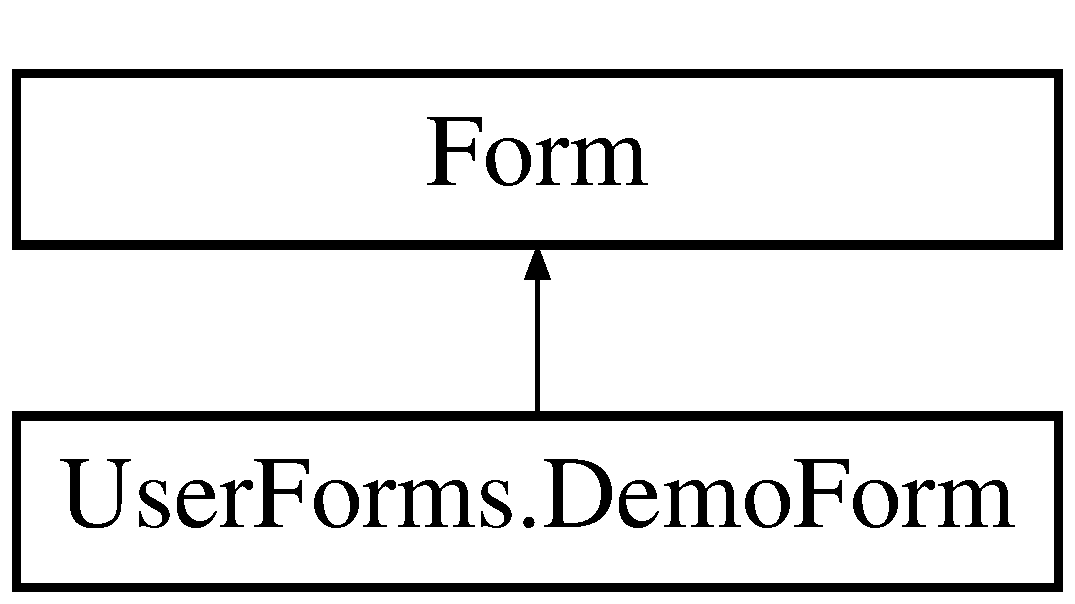
\includegraphics[height=2.000000cm]{class_user_forms_1_1_demo_form}
\end{center}
\end{figure}
\subsection*{Public Member Functions}
\begin{DoxyCompactItemize}
\item 
\hyperlink{class_user_forms_1_1_demo_form_a9ef677039850f5ac014ad27d1aa95160}{Demo\+Form} ()
\end{DoxyCompactItemize}
\subsection*{Protected Member Functions}
\begin{DoxyCompactItemize}
\item 
override void \hyperlink{class_user_forms_1_1_demo_form_a1dd0d43c1b10b64a4591d4b6235f0148}{Dispose} (bool disposing)
\begin{DoxyCompactList}\small\item\em Clean up any resources being used. \end{DoxyCompactList}\end{DoxyCompactItemize}


\subsection{Detailed Description}
Interactive visual demo of the Game of Life on a rectangular playground. This is not a platform for programming or serious experiments. 



Definition at line 14 of file Demo\+Form.\+cs.



\subsection{Constructor \& Destructor Documentation}
\hypertarget{class_user_forms_1_1_demo_form_a9ef677039850f5ac014ad27d1aa95160}{}\index{User\+Forms\+::\+Demo\+Form@{User\+Forms\+::\+Demo\+Form}!Demo\+Form@{Demo\+Form}}
\index{Demo\+Form@{Demo\+Form}!User\+Forms\+::\+Demo\+Form@{User\+Forms\+::\+Demo\+Form}}
\subsubsection[{Demo\+Form()}]{\setlength{\rightskip}{0pt plus 5cm}User\+Forms.\+Demo\+Form.\+Demo\+Form (
\begin{DoxyParamCaption}
{}
\end{DoxyParamCaption}
)}\label{class_user_forms_1_1_demo_form_a9ef677039850f5ac014ad27d1aa95160}


Definition at line 23 of file Demo\+Form.\+cs.



\subsection{Member Function Documentation}
\hypertarget{class_user_forms_1_1_demo_form_a1dd0d43c1b10b64a4591d4b6235f0148}{}\index{User\+Forms\+::\+Demo\+Form@{User\+Forms\+::\+Demo\+Form}!Dispose@{Dispose}}
\index{Dispose@{Dispose}!User\+Forms\+::\+Demo\+Form@{User\+Forms\+::\+Demo\+Form}}
\subsubsection[{Dispose(bool disposing)}]{\setlength{\rightskip}{0pt plus 5cm}override void User\+Forms.\+Demo\+Form.\+Dispose (
\begin{DoxyParamCaption}
\item[{bool}]{disposing}
\end{DoxyParamCaption}
)\hspace{0.3cm}{\ttfamily [protected]}}\label{class_user_forms_1_1_demo_form_a1dd0d43c1b10b64a4591d4b6235f0148}


Clean up any resources being used. 


\begin{DoxyParams}{Parameters}
{\em disposing} & true if managed resources should be disposed; otherwise, false.\\
\hline
\end{DoxyParams}


Definition at line 14 of file Demo\+Form.\+Designer.\+cs.



The documentation for this class was generated from the following files\+:\begin{DoxyCompactItemize}
\item 
C\+:/\+Martin/\+M\+F\+F/\+\_\+baka/\+Martin\+Dvorak/\+User\+Forms/\hyperlink{_demo_form_8cs}{Demo\+Form.\+cs}\item 
C\+:/\+Martin/\+M\+F\+F/\+\_\+baka/\+Martin\+Dvorak/\+User\+Forms/\hyperlink{_demo_form_8_designer_8cs}{Demo\+Form.\+Designer.\+cs}\end{DoxyCompactItemize}

\hypertarget{class_cellular_1_1_elementary_automaton}{}\section{Cellular.\+Elementary\+Automaton Class Reference}
\label{class_cellular_1_1_elementary_automaton}\index{Cellular.\+Elementary\+Automaton@{Cellular.\+Elementary\+Automaton}}


Class representing 256 elementary C\+A with firmly set borders. This specific implementation calculates every bit separately.  


Inheritance diagram for Cellular.\+Elementary\+Automaton\+:\begin{figure}[H]
\begin{center}
\leavevmode
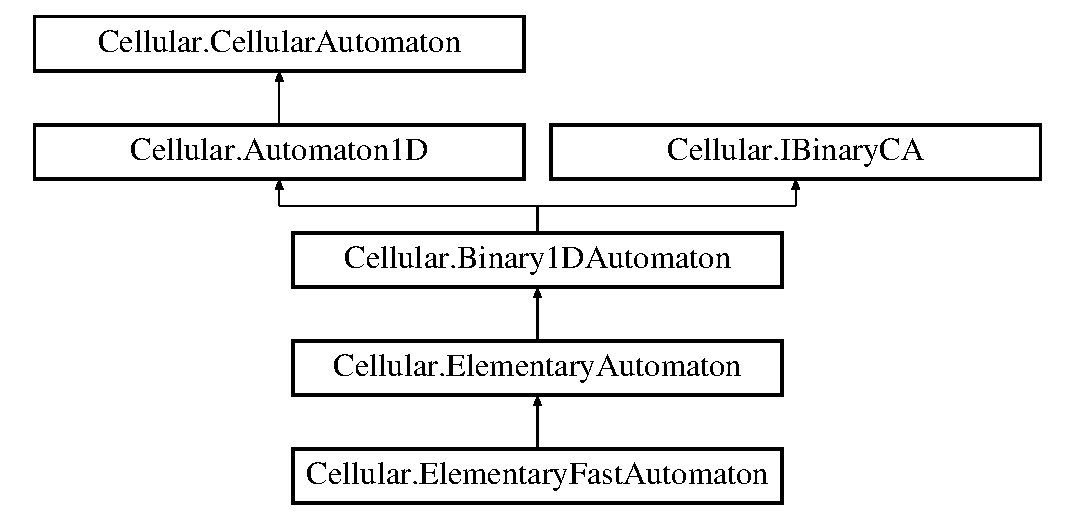
\includegraphics[height=5.000000cm]{class_cellular_1_1_elementary_automaton}
\end{center}
\end{figure}
\subsection*{Public Member Functions}
\begin{DoxyCompactItemize}
\item 
\hyperlink{class_cellular_1_1_elementary_automaton_a3102fe9e27bc0b89dd69b1c8d1298594}{Elementary\+Automaton} ()
\begin{DoxyCompactList}\small\item\em Creates a new basic C\+A of size 100 with 000...00100...000 as its initial state. The new C\+A will use rule No.\+30 \+: asymmetric, pseudo-\/chaotic behaviour. \end{DoxyCompactList}\item 
\hyperlink{class_cellular_1_1_elementary_automaton_adb0c84746e3c2d1c65010f506d010e94}{Elementary\+Automaton} (int \hyperlink{class_cellular_1_1_automaton1_d_a915129ccf0f1e7092844c99ce6a28e5b}{size})
\begin{DoxyCompactList}\small\item\em Creates a new basic C\+A with 000...00100...000 as its initial state. The new C\+A will use rule No.\+30 \+: asymmetric, pseudo-\/chaotic behaviour. \end{DoxyCompactList}\item 
\hyperlink{class_cellular_1_1_elementary_automaton_aa8326e685de0a177a5125625280fdde1}{Elementary\+Automaton} (byte rule\+No, int \hyperlink{class_cellular_1_1_automaton1_d_a915129ccf0f1e7092844c99ce6a28e5b}{size})
\begin{DoxyCompactList}\small\item\em Creates a new basic C\+A with given rule and 000...00100...000 as its initial state. \end{DoxyCompactList}\item 
\hyperlink{class_cellular_1_1_elementary_automaton_aa5d649a5cc42560eede2ac3c96199f7b}{Elementary\+Automaton} (byte rule\+No, Bit\+Array \hyperlink{all__1_8js_ae8b87ff4be2ae1dd5267342795263360}{initial\+State})
\begin{DoxyCompactList}\small\item\em Creates a new basic C\+A with given rule and initial state. \end{DoxyCompactList}\item 
\hyperlink{class_cellular_1_1_elementary_automaton_a64849d809eb4962cb09b5263f3227457}{Elementary\+Automaton} (byte rule\+No, int \hyperlink{class_cellular_1_1_automaton1_d_a915129ccf0f1e7092844c99ce6a28e5b}{size}, Random rnd)
\begin{DoxyCompactList}\small\item\em Creates a new basic C\+A. \end{DoxyCompactList}\item 
override void \hyperlink{class_cellular_1_1_elementary_automaton_adae7c322e4c7cd00cd0534a23d1abfa4}{Step} ()
\begin{DoxyCompactList}\small\item\em Performs one step of the cellular automaton. Always calls {\ttfamily \hyperlink{class_cellular_1_1_cellular_automaton_aa70848d58015575974bc875ac5a89ae7}{Cellular\+Automaton.\+Step()}}. \end{DoxyCompactList}\item 
override int \hyperlink{class_cellular_1_1_elementary_automaton_abaa1bb77264571ec245155f079fe1ff0}{Get\+Hash\+Code} ()
\item 
override object \hyperlink{class_cellular_1_1_elementary_automaton_ada4ddee98167e8f4f4b6dea1f7563b47}{Clone} ()
\begin{DoxyCompactList}\small\item\em Creates an appropriate copy of the C\+A. Its type and the specific rule are always preserved. However, the time (number of steps executed on the specific instance) is set back to 0. \end{DoxyCompactList}\item 
override string \hyperlink{class_cellular_1_1_elementary_automaton_a812677139d560e2c600226361b785995}{Tell\+Type} ()
\begin{DoxyCompactList}\small\item\em Announces the runtime type of the C\+A including info about its rule. It serves for debugging purposes. \end{DoxyCompactList}\item 
\hyperlink{class_cellular_1_1_binary_range_automaton}{Binary\+Range\+Automaton} \hyperlink{class_cellular_1_1_elementary_automaton_aef244148e0234495c1f0afaef7f22e28}{Convert\+To\+Range\+N} ()
\begin{DoxyCompactList}\small\item\em Creates an equivalent C\+A, which only has a \char`\"{}more general\char`\"{} type. \end{DoxyCompactList}\item 
\hyperlink{class_cellular_1_1_binary_range_cyclic_automaton}{Binary\+Range\+Cyclic\+Automaton} \hyperlink{class_cellular_1_1_elementary_automaton_a8876a09ba28af93b0e5163eef3cbe79e}{Convert\+To\+Cyclic\+N} ()
\begin{DoxyCompactList}\small\item\em Creates a new C\+A with the same state and the same rule, but connected boundaries. \end{DoxyCompactList}\end{DoxyCompactItemize}
\subsection*{Protected Member Functions}
\begin{DoxyCompactItemize}
\item 
void \hyperlink{class_cellular_1_1_elementary_automaton_ac5b75fb02cff4d4697e3e04cc9849154}{rule\+From\+Number} (byte rule\+No)
\item 
override \hyperlink{interface_cellular_1_1_i_binary_c_a}{I\+Binary\+C\+A} \hyperlink{class_cellular_1_1_elementary_automaton_ae2a263ffe6e021daff6a4a6c45555f6c}{clone\+Template} (Bit\+Array new\+Instance\+State)
\end{DoxyCompactItemize}
\subsection*{Protected Attributes}
\begin{DoxyCompactItemize}
\item 
byte \hyperlink{class_cellular_1_1_elementary_automaton_aa9221b2c09faebf1dd67ba75194b15f8}{rule\+Number}
\item 
bool\mbox{[},,\mbox{]} \hyperlink{class_cellular_1_1_elementary_automaton_a7de75f196155059435ac9098aa6b2a52}{rule}
\end{DoxyCompactItemize}


\subsection{Detailed Description}
Class representing 256 elementary C\+A with firmly set borders. This specific implementation calculates every bit separately. 



Definition at line 10 of file Elementary\+Automaton.\+cs.



\subsection{Constructor \& Destructor Documentation}
\hypertarget{class_cellular_1_1_elementary_automaton_a3102fe9e27bc0b89dd69b1c8d1298594}{}\index{Cellular\+::\+Elementary\+Automaton@{Cellular\+::\+Elementary\+Automaton}!Elementary\+Automaton@{Elementary\+Automaton}}
\index{Elementary\+Automaton@{Elementary\+Automaton}!Cellular\+::\+Elementary\+Automaton@{Cellular\+::\+Elementary\+Automaton}}
\subsubsection[{Elementary\+Automaton()}]{\setlength{\rightskip}{0pt plus 5cm}Cellular.\+Elementary\+Automaton.\+Elementary\+Automaton (
\begin{DoxyParamCaption}
{}
\end{DoxyParamCaption}
)}\label{class_cellular_1_1_elementary_automaton_a3102fe9e27bc0b89dd69b1c8d1298594}


Creates a new basic C\+A of size 100 with 000...00100...000 as its initial state. The new C\+A will use rule No.\+30 \+: asymmetric, pseudo-\/chaotic behaviour. 



Definition at line 19 of file Elementary\+Automaton.\+cs.

\hypertarget{class_cellular_1_1_elementary_automaton_adb0c84746e3c2d1c65010f506d010e94}{}\index{Cellular\+::\+Elementary\+Automaton@{Cellular\+::\+Elementary\+Automaton}!Elementary\+Automaton@{Elementary\+Automaton}}
\index{Elementary\+Automaton@{Elementary\+Automaton}!Cellular\+::\+Elementary\+Automaton@{Cellular\+::\+Elementary\+Automaton}}
\subsubsection[{Elementary\+Automaton(int size)}]{\setlength{\rightskip}{0pt plus 5cm}Cellular.\+Elementary\+Automaton.\+Elementary\+Automaton (
\begin{DoxyParamCaption}
\item[{int}]{size}
\end{DoxyParamCaption}
)}\label{class_cellular_1_1_elementary_automaton_adb0c84746e3c2d1c65010f506d010e94}


Creates a new basic C\+A with 000...00100...000 as its initial state. The new C\+A will use rule No.\+30 \+: asymmetric, pseudo-\/chaotic behaviour. 


\begin{DoxyParams}{Parameters}
{\em size} & The size of the new C\+A.\\
\hline
\end{DoxyParams}


Definition at line 26 of file Elementary\+Automaton.\+cs.

\hypertarget{class_cellular_1_1_elementary_automaton_aa8326e685de0a177a5125625280fdde1}{}\index{Cellular\+::\+Elementary\+Automaton@{Cellular\+::\+Elementary\+Automaton}!Elementary\+Automaton@{Elementary\+Automaton}}
\index{Elementary\+Automaton@{Elementary\+Automaton}!Cellular\+::\+Elementary\+Automaton@{Cellular\+::\+Elementary\+Automaton}}
\subsubsection[{Elementary\+Automaton(byte rule\+No, int size)}]{\setlength{\rightskip}{0pt plus 5cm}Cellular.\+Elementary\+Automaton.\+Elementary\+Automaton (
\begin{DoxyParamCaption}
\item[{byte}]{rule\+No, }
\item[{int}]{size}
\end{DoxyParamCaption}
)}\label{class_cellular_1_1_elementary_automaton_aa8326e685de0a177a5125625280fdde1}


Creates a new basic C\+A with given rule and 000...00100...000 as its initial state. 


\begin{DoxyParams}{Parameters}
{\em rule\+No} & The code of the elementary rule (from 0 to 255).\\
\hline
{\em size} & The size of the new C\+A.\\
\hline
\end{DoxyParams}


Definition at line 33 of file Elementary\+Automaton.\+cs.

\hypertarget{class_cellular_1_1_elementary_automaton_aa5d649a5cc42560eede2ac3c96199f7b}{}\index{Cellular\+::\+Elementary\+Automaton@{Cellular\+::\+Elementary\+Automaton}!Elementary\+Automaton@{Elementary\+Automaton}}
\index{Elementary\+Automaton@{Elementary\+Automaton}!Cellular\+::\+Elementary\+Automaton@{Cellular\+::\+Elementary\+Automaton}}
\subsubsection[{Elementary\+Automaton(byte rule\+No, Bit\+Array initial\+State)}]{\setlength{\rightskip}{0pt plus 5cm}Cellular.\+Elementary\+Automaton.\+Elementary\+Automaton (
\begin{DoxyParamCaption}
\item[{byte}]{rule\+No, }
\item[{Bit\+Array}]{initial\+State}
\end{DoxyParamCaption}
)}\label{class_cellular_1_1_elementary_automaton_aa5d649a5cc42560eede2ac3c96199f7b}


Creates a new basic C\+A with given rule and initial state. 


\begin{DoxyParams}{Parameters}
{\em rule\+No} & The code of the elementary rule (from 0 to 255).\\
\hline
{\em initial\+State} & A {\ttfamily Bit\+Array} describing the initial state of the C\+A. This also determines the size of the new C\+A.\\
\hline
\end{DoxyParams}


Definition at line 45 of file Elementary\+Automaton.\+cs.

\hypertarget{class_cellular_1_1_elementary_automaton_a64849d809eb4962cb09b5263f3227457}{}\index{Cellular\+::\+Elementary\+Automaton@{Cellular\+::\+Elementary\+Automaton}!Elementary\+Automaton@{Elementary\+Automaton}}
\index{Elementary\+Automaton@{Elementary\+Automaton}!Cellular\+::\+Elementary\+Automaton@{Cellular\+::\+Elementary\+Automaton}}
\subsubsection[{Elementary\+Automaton(byte rule\+No, int size, Random rnd)}]{\setlength{\rightskip}{0pt plus 5cm}Cellular.\+Elementary\+Automaton.\+Elementary\+Automaton (
\begin{DoxyParamCaption}
\item[{byte}]{rule\+No, }
\item[{int}]{size, }
\item[{Random}]{rnd}
\end{DoxyParamCaption}
)}\label{class_cellular_1_1_elementary_automaton_a64849d809eb4962cb09b5263f3227457}


Creates a new basic C\+A. 


\begin{DoxyParams}{Parameters}
{\em rule\+No} & The code of the elementary rule (from 0 to 255).\\
\hline
{\em size} & The size of the new C\+A.\\
\hline
{\em rnd} & Pseudo\+R\+N\+G instance that will be used to generate the original state.\\
\hline
\end{DoxyParams}


Definition at line 57 of file Elementary\+Automaton.\+cs.



\subsection{Member Function Documentation}
\hypertarget{class_cellular_1_1_elementary_automaton_ada4ddee98167e8f4f4b6dea1f7563b47}{}\index{Cellular\+::\+Elementary\+Automaton@{Cellular\+::\+Elementary\+Automaton}!Clone@{Clone}}
\index{Clone@{Clone}!Cellular\+::\+Elementary\+Automaton@{Cellular\+::\+Elementary\+Automaton}}
\subsubsection[{Clone()}]{\setlength{\rightskip}{0pt plus 5cm}override object Cellular.\+Elementary\+Automaton.\+Clone (
\begin{DoxyParamCaption}
{}
\end{DoxyParamCaption}
)\hspace{0.3cm}{\ttfamily [virtual]}}\label{class_cellular_1_1_elementary_automaton_ada4ddee98167e8f4f4b6dea1f7563b47}


Creates an appropriate copy of the C\+A. Its type and the specific rule are always preserved. However, the time (number of steps executed on the specific instance) is set back to 0. 

\begin{DoxyReturn}{Returns}
A copy of the {\ttfamily \hyperlink{class_cellular_1_1_cellular_automaton}{Cellular\+Automaton}} as an {\ttfamily Object}
\end{DoxyReturn}


Implements \hyperlink{class_cellular_1_1_cellular_automaton_affd487b397cdbbbb1982815bbcd8e7d3}{Cellular.\+Cellular\+Automaton}.



Reimplemented in \hyperlink{class_cellular_1_1_elementary_fast_automaton_a98bbdcade0ac93dd0fbc96ba253c2978}{Cellular.\+Elementary\+Fast\+Automaton}.



Definition at line 103 of file Elementary\+Automaton.\+cs.

\hypertarget{class_cellular_1_1_elementary_automaton_ae2a263ffe6e021daff6a4a6c45555f6c}{}\index{Cellular\+::\+Elementary\+Automaton@{Cellular\+::\+Elementary\+Automaton}!clone\+Template@{clone\+Template}}
\index{clone\+Template@{clone\+Template}!Cellular\+::\+Elementary\+Automaton@{Cellular\+::\+Elementary\+Automaton}}
\subsubsection[{clone\+Template(\+Bit\+Array new\+Instance\+State)}]{\setlength{\rightskip}{0pt plus 5cm}override {\bf I\+Binary\+C\+A} Cellular.\+Elementary\+Automaton.\+clone\+Template (
\begin{DoxyParamCaption}
\item[{Bit\+Array}]{new\+Instance\+State}
\end{DoxyParamCaption}
)\hspace{0.3cm}{\ttfamily [protected]}, {\ttfamily [virtual]}}\label{class_cellular_1_1_elementary_automaton_ae2a263ffe6e021daff6a4a6c45555f6c}


Implements \hyperlink{class_cellular_1_1_binary1_d_automaton_a38ac5ae077c5d31356d278247fbab40a}{Cellular.\+Binary1\+D\+Automaton}.



Reimplemented in \hyperlink{class_cellular_1_1_elementary_fast_automaton_a95b5abc22d134cb9640b56a0a70c1454}{Cellular.\+Elementary\+Fast\+Automaton}.



Definition at line 108 of file Elementary\+Automaton.\+cs.

\hypertarget{class_cellular_1_1_elementary_automaton_a8876a09ba28af93b0e5163eef3cbe79e}{}\index{Cellular\+::\+Elementary\+Automaton@{Cellular\+::\+Elementary\+Automaton}!Convert\+To\+Cyclic\+N@{Convert\+To\+Cyclic\+N}}
\index{Convert\+To\+Cyclic\+N@{Convert\+To\+Cyclic\+N}!Cellular\+::\+Elementary\+Automaton@{Cellular\+::\+Elementary\+Automaton}}
\subsubsection[{Convert\+To\+Cyclic\+N()}]{\setlength{\rightskip}{0pt plus 5cm}{\bf Binary\+Range\+Cyclic\+Automaton} Cellular.\+Elementary\+Automaton.\+Convert\+To\+Cyclic\+N (
\begin{DoxyParamCaption}
{}
\end{DoxyParamCaption}
)}\label{class_cellular_1_1_elementary_automaton_a8876a09ba28af93b0e5163eef3cbe79e}


Creates a new C\+A with the same state and the same rule, but connected boundaries. 

\begin{DoxyReturn}{Returns}
A modified \char`\"{}copy\char`\"{} of this C\+A as {\ttfamily \hyperlink{class_cellular_1_1_binary_range_cyclic_automaton}{Binary\+Range\+Cyclic\+Automaton}}.
\end{DoxyReturn}


Definition at line 143 of file Elementary\+Automaton.\+cs.

\hypertarget{class_cellular_1_1_elementary_automaton_aef244148e0234495c1f0afaef7f22e28}{}\index{Cellular\+::\+Elementary\+Automaton@{Cellular\+::\+Elementary\+Automaton}!Convert\+To\+Range\+N@{Convert\+To\+Range\+N}}
\index{Convert\+To\+Range\+N@{Convert\+To\+Range\+N}!Cellular\+::\+Elementary\+Automaton@{Cellular\+::\+Elementary\+Automaton}}
\subsubsection[{Convert\+To\+Range\+N()}]{\setlength{\rightskip}{0pt plus 5cm}{\bf Binary\+Range\+Automaton} Cellular.\+Elementary\+Automaton.\+Convert\+To\+Range\+N (
\begin{DoxyParamCaption}
{}
\end{DoxyParamCaption}
)}\label{class_cellular_1_1_elementary_automaton_aef244148e0234495c1f0afaef7f22e28}


Creates an equivalent C\+A, which only has a \char`\"{}more general\char`\"{} type. 

\begin{DoxyReturn}{Returns}
A \char`\"{}copy\char`\"{} of this C\+A as {\ttfamily \hyperlink{class_cellular_1_1_binary_range_automaton}{Binary\+Range\+Automaton}}.
\end{DoxyReturn}


Definition at line 134 of file Elementary\+Automaton.\+cs.

\hypertarget{class_cellular_1_1_elementary_automaton_abaa1bb77264571ec245155f079fe1ff0}{}\index{Cellular\+::\+Elementary\+Automaton@{Cellular\+::\+Elementary\+Automaton}!Get\+Hash\+Code@{Get\+Hash\+Code}}
\index{Get\+Hash\+Code@{Get\+Hash\+Code}!Cellular\+::\+Elementary\+Automaton@{Cellular\+::\+Elementary\+Automaton}}
\subsubsection[{Get\+Hash\+Code()}]{\setlength{\rightskip}{0pt plus 5cm}override int Cellular.\+Elementary\+Automaton.\+Get\+Hash\+Code (
\begin{DoxyParamCaption}
{}
\end{DoxyParamCaption}
)}\label{class_cellular_1_1_elementary_automaton_abaa1bb77264571ec245155f079fe1ff0}


Definition at line 98 of file Elementary\+Automaton.\+cs.

\hypertarget{class_cellular_1_1_elementary_automaton_ac5b75fb02cff4d4697e3e04cc9849154}{}\index{Cellular\+::\+Elementary\+Automaton@{Cellular\+::\+Elementary\+Automaton}!rule\+From\+Number@{rule\+From\+Number}}
\index{rule\+From\+Number@{rule\+From\+Number}!Cellular\+::\+Elementary\+Automaton@{Cellular\+::\+Elementary\+Automaton}}
\subsubsection[{rule\+From\+Number(byte rule\+No)}]{\setlength{\rightskip}{0pt plus 5cm}void Cellular.\+Elementary\+Automaton.\+rule\+From\+Number (
\begin{DoxyParamCaption}
\item[{byte}]{rule\+No}
\end{DoxyParamCaption}
)\hspace{0.3cm}{\ttfamily [protected]}}\label{class_cellular_1_1_elementary_automaton_ac5b75fb02cff4d4697e3e04cc9849154}


Definition at line 63 of file Elementary\+Automaton.\+cs.

\hypertarget{class_cellular_1_1_elementary_automaton_adae7c322e4c7cd00cd0534a23d1abfa4}{}\index{Cellular\+::\+Elementary\+Automaton@{Cellular\+::\+Elementary\+Automaton}!Step@{Step}}
\index{Step@{Step}!Cellular\+::\+Elementary\+Automaton@{Cellular\+::\+Elementary\+Automaton}}
\subsubsection[{Step()}]{\setlength{\rightskip}{0pt plus 5cm}override void Cellular.\+Elementary\+Automaton.\+Step (
\begin{DoxyParamCaption}
{}
\end{DoxyParamCaption}
)}\label{class_cellular_1_1_elementary_automaton_adae7c322e4c7cd00cd0534a23d1abfa4}


Performs one step of the cellular automaton. Always calls {\ttfamily \hyperlink{class_cellular_1_1_cellular_automaton_aa70848d58015575974bc875ac5a89ae7}{Cellular\+Automaton.\+Step()}}. 



Implements \hyperlink{interface_cellular_1_1_i_binary_c_a_a6a04c7374538c49df07efa176e0dd3c3}{Cellular.\+I\+Binary\+C\+A}.



Definition at line 83 of file Elementary\+Automaton.\+cs.

\hypertarget{class_cellular_1_1_elementary_automaton_a812677139d560e2c600226361b785995}{}\index{Cellular\+::\+Elementary\+Automaton@{Cellular\+::\+Elementary\+Automaton}!Tell\+Type@{Tell\+Type}}
\index{Tell\+Type@{Tell\+Type}!Cellular\+::\+Elementary\+Automaton@{Cellular\+::\+Elementary\+Automaton}}
\subsubsection[{Tell\+Type()}]{\setlength{\rightskip}{0pt plus 5cm}override string Cellular.\+Elementary\+Automaton.\+Tell\+Type (
\begin{DoxyParamCaption}
{}
\end{DoxyParamCaption}
)}\label{class_cellular_1_1_elementary_automaton_a812677139d560e2c600226361b785995}


Announces the runtime type of the C\+A including info about its rule. It serves for debugging purposes. 

\begin{DoxyReturn}{Returns}
The same string as calling {\ttfamily \hyperlink{class_cellular_1_1_cellular_automaton_abe4b92fd405530c8a08cc07a3a19fff4}{Cellular\+Automaton.\+Tell\+Type()}}.
\end{DoxyReturn}


Implements \hyperlink{interface_cellular_1_1_i_binary_c_a_aa67feabf5d1513aa74076d255c661948}{Cellular.\+I\+Binary\+C\+A}.



Definition at line 113 of file Elementary\+Automaton.\+cs.



\subsection{Member Data Documentation}
\hypertarget{class_cellular_1_1_elementary_automaton_a7de75f196155059435ac9098aa6b2a52}{}\index{Cellular\+::\+Elementary\+Automaton@{Cellular\+::\+Elementary\+Automaton}!rule@{rule}}
\index{rule@{rule}!Cellular\+::\+Elementary\+Automaton@{Cellular\+::\+Elementary\+Automaton}}
\subsubsection[{rule}]{\setlength{\rightskip}{0pt plus 5cm}bool \mbox{[}, ,\mbox{]} Cellular.\+Elementary\+Automaton.\+rule\hspace{0.3cm}{\ttfamily [protected]}}\label{class_cellular_1_1_elementary_automaton_a7de75f196155059435ac9098aa6b2a52}


Definition at line 13 of file Elementary\+Automaton.\+cs.

\hypertarget{class_cellular_1_1_elementary_automaton_aa9221b2c09faebf1dd67ba75194b15f8}{}\index{Cellular\+::\+Elementary\+Automaton@{Cellular\+::\+Elementary\+Automaton}!rule\+Number@{rule\+Number}}
\index{rule\+Number@{rule\+Number}!Cellular\+::\+Elementary\+Automaton@{Cellular\+::\+Elementary\+Automaton}}
\subsubsection[{rule\+Number}]{\setlength{\rightskip}{0pt plus 5cm}byte Cellular.\+Elementary\+Automaton.\+rule\+Number\hspace{0.3cm}{\ttfamily [protected]}}\label{class_cellular_1_1_elementary_automaton_aa9221b2c09faebf1dd67ba75194b15f8}


Definition at line 12 of file Elementary\+Automaton.\+cs.



The documentation for this class was generated from the following file\+:\begin{DoxyCompactItemize}
\item 
C\+:/\+Martin/\+M\+F\+F/\+\_\+baka/\+Martin\+Dvorak/\+Cellular/\hyperlink{_elementary_automaton_8cs}{Elementary\+Automaton.\+cs}\end{DoxyCompactItemize}

\input{class_cellular_1_1_elementary_automaton_fast}
\input{class_cellular_1_1_elementary_automaton_faster}
\input{class_cellular_1_1_elementary_automaton_parallel}
\input{class_testing_1_1_elementary_implementations_test}
\hypertarget{class_testing_1_1_elementary_time_measure}{}\section{Testing.\+Elementary\+Time\+Measure Class Reference}
\label{class_testing_1_1_elementary_time_measure}\index{Testing.\+Elementary\+Time\+Measure@{Testing.\+Elementary\+Time\+Measure}}


Simple test of how different classes are (in)efficient for implementing elementary C\+A rules.  


\subsection*{Static Public Member Functions}
\begin{DoxyCompactItemize}
\item 
static void \hyperlink{class_testing_1_1_elementary_time_measure_a7953a79dc736debab827b426e98d1d6e}{Run\+Test} ()
\end{DoxyCompactItemize}


\subsection{Detailed Description}
Simple test of how different classes are (in)efficient for implementing elementary C\+A rules. 



Definition at line 11 of file Elementary\+Time\+Measure.\+cs.



\subsection{Member Function Documentation}
\hypertarget{class_testing_1_1_elementary_time_measure_a7953a79dc736debab827b426e98d1d6e}{}\index{Testing\+::\+Elementary\+Time\+Measure@{Testing\+::\+Elementary\+Time\+Measure}!Run\+Test@{Run\+Test}}
\index{Run\+Test@{Run\+Test}!Testing\+::\+Elementary\+Time\+Measure@{Testing\+::\+Elementary\+Time\+Measure}}
\subsubsection[{Run\+Test()}]{\setlength{\rightskip}{0pt plus 5cm}static void Testing.\+Elementary\+Time\+Measure.\+Run\+Test (
\begin{DoxyParamCaption}
{}
\end{DoxyParamCaption}
)\hspace{0.3cm}{\ttfamily [static]}}\label{class_testing_1_1_elementary_time_measure_a7953a79dc736debab827b426e98d1d6e}


Definition at line 17 of file Elementary\+Time\+Measure.\+cs.



The documentation for this class was generated from the following file\+:\begin{DoxyCompactItemize}
\item 
C\+:/\+Martin/\+M\+F\+F/\+\_\+baka/\+Martin\+Dvorak/\+Testing/\hyperlink{_elementary_time_measure_8cs}{Elementary\+Time\+Measure.\+cs}\end{DoxyCompactItemize}

\input{class_crypto_1_1_encrypter_reversible_c_a}
\input{class_cryptography_unit_tests_1_1_encrypter_reversible_c_atests}
\input{class_crypto_1_1_encrypter_stream_c_a}
\input{class_cryptography_unit_tests_1_1_encrypter_stream_c_atests}
\input{class_crypto_1_1_encryption_provider}
\hypertarget{class_crypto_1_1_export}{}\section{Crypto.\+Export Class Reference}
\label{class_crypto_1_1_export}\index{Crypto.\+Export@{Crypto.\+Export}}


Public static class that gives access to our cryptographical tools. This class is made to be used from any assembly.  


\subsection*{Static Public Member Functions}
\begin{DoxyCompactItemize}
\item 
static \hyperlink{interface_crypto_1_1_i_key_extender}{I\+Key\+Extender} \hyperlink{class_crypto_1_1_export_a32a0f5d57f02adbe05c8b9c6ca2d30fe}{Get\+Key\+Extender} ()
\begin{DoxyCompactList}\small\item\em Exports a key extender for use by any external program. \end{DoxyCompactList}\item 
static \hyperlink{class_crypto_1_1_encrypter_wrapper}{Encrypter\+Wrapper} \hyperlink{class_crypto_1_1_export_afbdd82980115f75656284bfc1cedaf71}{Get\+Encrypter\+Stream\+C\+A} ()
\begin{DoxyCompactList}\small\item\em Exports a ready-\/to-\/use encrypter/decrypter for use by any external program. This uses C\+A-\/based key extender inside. \end{DoxyCompactList}\item 
static \hyperlink{class_crypto_1_1_encrypter_wrapper}{Encrypter\+Wrapper} \hyperlink{class_crypto_1_1_export_a724346aca326fe3f8725eb7c7c3a4390}{Get\+Encrypter\+Reversible\+C\+A} ()
\begin{DoxyCompactList}\small\item\em Exports a ready-\/to-\/use encrypter/decrypter for use by any external program. This uses a reversible C\+A inside. \end{DoxyCompactList}\end{DoxyCompactItemize}


\subsection{Detailed Description}
Public static class that gives access to our cryptographical tools. This class is made to be used from any assembly. 



Definition at line 9 of file Export.\+cs.



\subsection{Member Function Documentation}
\hypertarget{class_crypto_1_1_export_a724346aca326fe3f8725eb7c7c3a4390}{}\index{Crypto\+::\+Export@{Crypto\+::\+Export}!Get\+Encrypter\+Reversible\+C\+A@{Get\+Encrypter\+Reversible\+C\+A}}
\index{Get\+Encrypter\+Reversible\+C\+A@{Get\+Encrypter\+Reversible\+C\+A}!Crypto\+::\+Export@{Crypto\+::\+Export}}
\subsubsection[{Get\+Encrypter\+Reversible\+C\+A()}]{\setlength{\rightskip}{0pt plus 5cm}static {\bf Encrypter\+Wrapper} Crypto.\+Export.\+Get\+Encrypter\+Reversible\+C\+A (
\begin{DoxyParamCaption}
{}
\end{DoxyParamCaption}
)\hspace{0.3cm}{\ttfamily [static]}}\label{class_crypto_1_1_export_a724346aca326fe3f8725eb7c7c3a4390}


Exports a ready-\/to-\/use encrypter/decrypter for use by any external program. This uses a reversible C\+A inside. 

\begin{DoxyReturn}{Returns}
Encrypter and decrypter.
\end{DoxyReturn}


Definition at line 42 of file Export.\+cs.

\hypertarget{class_crypto_1_1_export_afbdd82980115f75656284bfc1cedaf71}{}\index{Crypto\+::\+Export@{Crypto\+::\+Export}!Get\+Encrypter\+Stream\+C\+A@{Get\+Encrypter\+Stream\+C\+A}}
\index{Get\+Encrypter\+Stream\+C\+A@{Get\+Encrypter\+Stream\+C\+A}!Crypto\+::\+Export@{Crypto\+::\+Export}}
\subsubsection[{Get\+Encrypter\+Stream\+C\+A()}]{\setlength{\rightskip}{0pt plus 5cm}static {\bf Encrypter\+Wrapper} Crypto.\+Export.\+Get\+Encrypter\+Stream\+C\+A (
\begin{DoxyParamCaption}
{}
\end{DoxyParamCaption}
)\hspace{0.3cm}{\ttfamily [static]}}\label{class_crypto_1_1_export_afbdd82980115f75656284bfc1cedaf71}


Exports a ready-\/to-\/use encrypter/decrypter for use by any external program. This uses C\+A-\/based key extender inside. 

\begin{DoxyReturn}{Returns}
Encrypter and decrypter.
\end{DoxyReturn}


Definition at line 32 of file Export.\+cs.

\hypertarget{class_crypto_1_1_export_a32a0f5d57f02adbe05c8b9c6ca2d30fe}{}\index{Crypto\+::\+Export@{Crypto\+::\+Export}!Get\+Key\+Extender@{Get\+Key\+Extender}}
\index{Get\+Key\+Extender@{Get\+Key\+Extender}!Crypto\+::\+Export@{Crypto\+::\+Export}}
\subsubsection[{Get\+Key\+Extender()}]{\setlength{\rightskip}{0pt plus 5cm}static {\bf I\+Key\+Extender} Crypto.\+Export.\+Get\+Key\+Extender (
\begin{DoxyParamCaption}
{}
\end{DoxyParamCaption}
)\hspace{0.3cm}{\ttfamily [static]}}\label{class_crypto_1_1_export_a32a0f5d57f02adbe05c8b9c6ca2d30fe}


Exports a key extender for use by any external program. 

\begin{DoxyReturn}{Returns}
Key extender.
\end{DoxyReturn}


Definition at line 22 of file Export.\+cs.



The documentation for this class was generated from the following file\+:\begin{DoxyCompactItemize}
\item 
C\+:/\+Martin/\+M\+F\+F/\+\_\+baka/\+Martin\+Dvorak/\+Crypto/\hyperlink{_export_8cs}{Export.\+cs}\end{DoxyCompactItemize}

\hypertarget{class_crypto_1_1_factory}{}\section{Crypto.\+Factory Class Reference}
\label{class_crypto_1_1_factory}\index{Crypto.\+Factory@{Crypto.\+Factory}}


\hyperlink{class_crypto_1_1_factory}{Factory} class containing methods for building cellular automata and key extenders from textual description. Sometimes used together with {\ttfamily Cellular\+Automaton.\+Tell\+Type()} resp. {\ttfamily I\+Binary\+C\+A.\+Tell\+Type()} method as a replacement for missing serialization / deserialization features.  


\subsection*{Static Public Member Functions}
\begin{DoxyCompactItemize}
\item 
static \hyperlink{interface_cellular_1_1_i_binary_c_a}{I\+Binary\+C\+A} \hyperlink{class_crypto_1_1_factory_abe3a27bbc69843d3c912605709b75715}{Create\+Automaton} (string description)
\begin{DoxyCompactList}\small\item\em Creates a single binary C\+A from a description. \end{DoxyCompactList}\item 
static \hyperlink{class_crypto_1_1_key_extender_abstract_d}{Key\+Extender\+Abstract\+D} \hyperlink{class_crypto_1_1_factory_aec31ee8205c68b93aa3581aa4d8486d0}{Create\+Extender} (string description)
\begin{DoxyCompactList}\small\item\em Creates a key extender together with its C\+A from one description. \end{DoxyCompactList}\item 
static List$<$ \hyperlink{class_crypto_1_1_key_extender_abstract_d}{Key\+Extender\+Abstract\+D} $>$ \hyperlink{class_crypto_1_1_factory_abd5015e25ff66c3cf46bab4d67e60ce5}{Gather\+Successful\+Extenders} (string directory)
\begin{DoxyCompactList}\small\item\em Gathers successful key extenders from all files in given directory. \end{DoxyCompactList}\end{DoxyCompactItemize}


\subsection{Detailed Description}
\hyperlink{class_crypto_1_1_factory}{Factory} class containing methods for building cellular automata and key extenders from textual description. Sometimes used together with {\ttfamily Cellular\+Automaton.\+Tell\+Type()} resp. {\ttfamily I\+Binary\+C\+A.\+Tell\+Type()} method as a replacement for missing serialization / deserialization features. 



Definition at line 13 of file Factory.\+cs.



\subsection{Member Function Documentation}
\hypertarget{class_crypto_1_1_factory_abe3a27bbc69843d3c912605709b75715}{}\index{Crypto\+::\+Factory@{Crypto\+::\+Factory}!Create\+Automaton@{Create\+Automaton}}
\index{Create\+Automaton@{Create\+Automaton}!Crypto\+::\+Factory@{Crypto\+::\+Factory}}
\subsubsection[{Create\+Automaton(string description)}]{\setlength{\rightskip}{0pt plus 5cm}static {\bf I\+Binary\+C\+A} Crypto.\+Factory.\+Create\+Automaton (
\begin{DoxyParamCaption}
\item[{string}]{description}
\end{DoxyParamCaption}
)\hspace{0.3cm}{\ttfamily [static]}}\label{class_crypto_1_1_factory_abe3a27bbc69843d3c912605709b75715}


Creates a single binary C\+A from a description. 


\begin{DoxyParams}{Parameters}
{\em description} & Descrition of the C\+A -\/ output from {\ttfamily Tell\+Type()}.\\
\hline
\end{DoxyParams}
\begin{DoxyReturn}{Returns}

\end{DoxyReturn}


Definition at line 20 of file Factory.\+cs.

\hypertarget{class_crypto_1_1_factory_aec31ee8205c68b93aa3581aa4d8486d0}{}\index{Crypto\+::\+Factory@{Crypto\+::\+Factory}!Create\+Extender@{Create\+Extender}}
\index{Create\+Extender@{Create\+Extender}!Crypto\+::\+Factory@{Crypto\+::\+Factory}}
\subsubsection[{Create\+Extender(string description)}]{\setlength{\rightskip}{0pt plus 5cm}static {\bf Key\+Extender\+Abstract\+D} Crypto.\+Factory.\+Create\+Extender (
\begin{DoxyParamCaption}
\item[{string}]{description}
\end{DoxyParamCaption}
)\hspace{0.3cm}{\ttfamily [static]}}\label{class_crypto_1_1_factory_aec31ee8205c68b93aa3581aa4d8486d0}


Creates a key extender together with its C\+A from one description. 


\begin{DoxyParams}{Parameters}
{\em description} & Description of the key extender -\/ output from {\ttfamily Get\+Info()}.\\
\hline
\end{DoxyParams}
\begin{DoxyReturn}{Returns}
Object implementing \hyperlink{interface_crypto_1_1_i_key_extender}{I\+Key\+Extender} and \hyperlink{class_crypto_1_1_key_extender_abstract_d}{Key\+Extender\+Abstract\+D}.
\end{DoxyReturn}


Definition at line 74 of file Factory.\+cs.

\hypertarget{class_crypto_1_1_factory_abd5015e25ff66c3cf46bab4d67e60ce5}{}\index{Crypto\+::\+Factory@{Crypto\+::\+Factory}!Gather\+Successful\+Extenders@{Gather\+Successful\+Extenders}}
\index{Gather\+Successful\+Extenders@{Gather\+Successful\+Extenders}!Crypto\+::\+Factory@{Crypto\+::\+Factory}}
\subsubsection[{Gather\+Successful\+Extenders(string directory)}]{\setlength{\rightskip}{0pt plus 5cm}static List$<${\bf Key\+Extender\+Abstract\+D}$>$ Crypto.\+Factory.\+Gather\+Successful\+Extenders (
\begin{DoxyParamCaption}
\item[{string}]{directory}
\end{DoxyParamCaption}
)\hspace{0.3cm}{\ttfamily [static]}}\label{class_crypto_1_1_factory_abd5015e25ff66c3cf46bab4d67e60ce5}


Gathers successful key extenders from all files in given directory. 


\begin{DoxyParams}{Parameters}
{\em directory} & The directory with \char`\"{}.\+xca\char`\"{} files.\\
\hline
\end{DoxyParams}
\begin{DoxyReturn}{Returns}
List of (fully built) key extenders that were successful during previous runs of the genetic algorithm. 
\end{DoxyReturn}


Definition at line 106 of file Factory.\+cs.



The documentation for this class was generated from the following file\+:\begin{DoxyCompactItemize}
\item 
C\+:/\+Martin/\+M\+F\+F/\+\_\+baka/\+Martin\+Dvorak/\+Crypto/\hyperlink{_factory_8cs}{Factory.\+cs}\end{DoxyCompactItemize}

\hypertarget{class_testing_1_1_factory_test}{}\section{Testing.\+Factory\+Test Class Reference}
\label{class_testing_1_1_factory_test}\index{Testing.\+Factory\+Test@{Testing.\+Factory\+Test}}
\subsection*{Static Public Member Functions}
\begin{DoxyCompactItemize}
\item 
static void \hyperlink{class_testing_1_1_factory_test_a0efd537445b1aeb268bab3ee4be4ee1d}{Run\+Test} ()
\end{DoxyCompactItemize}


\subsection{Detailed Description}


Definition at line 6 of file Factory\+Test.\+cs.



\subsection{Member Function Documentation}
\hypertarget{class_testing_1_1_factory_test_a0efd537445b1aeb268bab3ee4be4ee1d}{}\index{Testing\+::\+Factory\+Test@{Testing\+::\+Factory\+Test}!Run\+Test@{Run\+Test}}
\index{Run\+Test@{Run\+Test}!Testing\+::\+Factory\+Test@{Testing\+::\+Factory\+Test}}
\subsubsection[{Run\+Test()}]{\setlength{\rightskip}{0pt plus 5cm}static void Testing.\+Factory\+Test.\+Run\+Test (
\begin{DoxyParamCaption}
{}
\end{DoxyParamCaption}
)\hspace{0.3cm}{\ttfamily [static]}}\label{class_testing_1_1_factory_test_a0efd537445b1aeb268bab3ee4be4ee1d}


Definition at line 8 of file Factory\+Test.\+cs.



The documentation for this class was generated from the following file\+:\begin{DoxyCompactItemize}
\item 
C\+:/\+Martin/\+M\+F\+F/\+\_\+baka/\+Martin\+Dvorak/\+Testing/\hyperlink{_factory_test_8cs}{Factory\+Test.\+cs}\end{DoxyCompactItemize}

\hypertarget{class_crypto_1_1_function_testing}{}\section{Crypto.\+Function\+Testing Class Reference}
\label{class_crypto_1_1_function_testing}\index{Crypto.\+Function\+Testing@{Crypto.\+Function\+Testing}}


Class for testing properties of key extending algorithms.  


\subsection*{Public Member Functions}
\begin{DoxyCompactItemize}
\item 
\hyperlink{class_crypto_1_1_function_testing_aa62a4223204dece41f9cc6fac9882834}{Function\+Testing} (bool use\+Levenshtein\+Distance=false)
\begin{DoxyCompactList}\small\item\em Creates a new instance of \hyperlink{class_crypto_1_1_function_testing}{Function\+Testing}. \end{DoxyCompactList}\item 
bool \hyperlink{class_crypto_1_1_function_testing_a3b4709eaa8b6f2a1a6c4fdb63eb46462}{is\+Levenshtein\+Inside} ()
\item 
double \hyperlink{class_crypto_1_1_function_testing_a4b3e7a81134c8e7337cf1b682f0be528}{Test\+Bit\+Change} (\hyperlink{interface_crypto_1_1_i_key_extender}{I\+Key\+Extender} algorithm, int ratio)
\begin{DoxyCompactList}\small\item\em Tests how much the output changes (on average) when the input changes in a single bit. \end{DoxyCompactList}\item 
double \hyperlink{class_crypto_1_1_function_testing_a847341d3b4a2f0e8ff155bc55ab3484f}{Test\+Average\+Distance} (\hyperlink{interface_crypto_1_1_i_key_extender}{I\+Key\+Extender} algorithm, int ratio)
\begin{DoxyCompactList}\small\item\em Tests average distance between two random results. \end{DoxyCompactList}\item 
double \hyperlink{class_crypto_1_1_function_testing_a11e504dfb7c6771eeb863f86a47a256d}{Test\+Largest\+Ball\+Exactly} (\hyperlink{interface_crypto_1_1_i_key_extender}{I\+Key\+Extender} algorithm)
\item 
double \hyperlink{class_crypto_1_1_function_testing_a937d2b136d13f2bc57ca3c03778c763e}{Test\+Largest\+Ball\+Approx} (\hyperlink{interface_crypto_1_1_i_key_extender}{I\+Key\+Extender} algorithm)
\item 
double \hyperlink{class_crypto_1_1_function_testing_acf3f02d42487bc168ce29e431ced28f6}{Test\+Random\+Sequences} (\hyperlink{interface_crypto_1_1_i_key_extender}{I\+Key\+Extender} algorithm, int ratio)
\begin{DoxyCompactList}\small\item\em Tests how much a random output resembles a pseudo-\/random binary sequence. \end{DoxyCompactList}\item 
double \hyperlink{class_crypto_1_1_function_testing_a9a647990f55860fb5c1703e4734a78e3}{Test\+Random\+Entropy} (\hyperlink{interface_crypto_1_1_i_key_extender}{I\+Key\+Extender} algorithm, int ratio)
\item 
double \hyperlink{class_crypto_1_1_function_testing_a29540726fa140a1cf1d2b637af553233}{Test\+Random\+Compression} (\hyperlink{interface_crypto_1_1_i_key_extender}{I\+Key\+Extender} algorithm, int ratio)
\item 
double \hyperlink{class_crypto_1_1_function_testing_a082771a8c25d3ac4b29906cbd73fb584}{Test\+Systematic\+Sequences} (\hyperlink{interface_crypto_1_1_i_key_extender}{I\+Key\+Extender} algorithm, int ratio)
\item 
double \hyperlink{class_crypto_1_1_function_testing_a38ff139e200ca760a150fd23f9b8c754}{Test\+Systematic\+Entropy} (\hyperlink{interface_crypto_1_1_i_key_extender}{I\+Key\+Extender} algorithm, int ratio)
\item 
double \hyperlink{class_crypto_1_1_function_testing_a3e1bedf80b820d257984dbae03d0e0e1}{Test\+Systematic\+Compression} (\hyperlink{interface_crypto_1_1_i_key_extender}{I\+Key\+Extender} algorithm, int ratio)
\end{DoxyCompactItemize}
\subsection*{Static Public Member Functions}
\begin{DoxyCompactItemize}
\item 
static double \hyperlink{class_crypto_1_1_function_testing_a643a83c8528858b2cfe531c176162796}{Hamming\+Distance} (Bit\+Array u, Bit\+Array v)
\begin{DoxyCompactList}\small\item\em Calculates the Hamming distance of two Bit\+Arrays of the same length. \end{DoxyCompactList}\item 
static double \hyperlink{class_crypto_1_1_function_testing_a88a16df256e6d63d43fbbb3b5c644f29}{Levenstein\+Distance} (Bit\+Array u, Bit\+Array v)
\begin{DoxyCompactList}\small\item\em Calculates the Levenshtein distance of two Bit\+Arrays of the same length. Sources\+: \href{https://en.wikipedia.org/wiki/Levenshtein_distance}{\tt https\+://en.\+wikipedia.\+org/wiki/\+Levenshtein\+\_\+distance} , \href{https://en.wikibooks.org/wiki/Algorithm_Implementation/Strings/Levenshtein_distance#C.23}{\tt https\+://en.\+wikibooks.\+org/wiki/\+Algorithm\+\_\+\+Implementation/\+Strings/\+Levenshtein\+\_\+distance\#\+C.\+23} \end{DoxyCompactList}\end{DoxyCompactItemize}


\subsection{Detailed Description}
Class for testing properties of key extending algorithms. 



Definition at line 11 of file Function\+Testing.\+cs.



\subsection{Constructor \& Destructor Documentation}
\hypertarget{class_crypto_1_1_function_testing_aa62a4223204dece41f9cc6fac9882834}{}\index{Crypto\+::\+Function\+Testing@{Crypto\+::\+Function\+Testing}!Function\+Testing@{Function\+Testing}}
\index{Function\+Testing@{Function\+Testing}!Crypto\+::\+Function\+Testing@{Crypto\+::\+Function\+Testing}}
\subsubsection[{Function\+Testing(bool use\+Levenshtein\+Distance=false)}]{\setlength{\rightskip}{0pt plus 5cm}Crypto.\+Function\+Testing.\+Function\+Testing (
\begin{DoxyParamCaption}
\item[{bool}]{use\+Levenshtein\+Distance = {\ttfamily false}}
\end{DoxyParamCaption}
)}\label{class_crypto_1_1_function_testing_aa62a4223204dece41f9cc6fac9882834}


Creates a new instance of \hyperlink{class_crypto_1_1_function_testing}{Function\+Testing}. 


\begin{DoxyParams}{Parameters}
{\em use\+Levenshtein\+Distance} & Should it use Levenshtein distance instead of Hamming distance? Note that Levenshtein distance is much slower to calculate. Default is Hamming distance.\\
\hline
\end{DoxyParams}


Definition at line 28 of file Function\+Testing.\+cs.



\subsection{Member Function Documentation}
\hypertarget{class_crypto_1_1_function_testing_a643a83c8528858b2cfe531c176162796}{}\index{Crypto\+::\+Function\+Testing@{Crypto\+::\+Function\+Testing}!Hamming\+Distance@{Hamming\+Distance}}
\index{Hamming\+Distance@{Hamming\+Distance}!Crypto\+::\+Function\+Testing@{Crypto\+::\+Function\+Testing}}
\subsubsection[{Hamming\+Distance(\+Bit\+Array u, Bit\+Array v)}]{\setlength{\rightskip}{0pt plus 5cm}static double Crypto.\+Function\+Testing.\+Hamming\+Distance (
\begin{DoxyParamCaption}
\item[{Bit\+Array}]{u, }
\item[{Bit\+Array}]{v}
\end{DoxyParamCaption}
)\hspace{0.3cm}{\ttfamily [static]}}\label{class_crypto_1_1_function_testing_a643a83c8528858b2cfe531c176162796}


Calculates the Hamming distance of two Bit\+Arrays of the same length. 


\begin{DoxyParams}{Parameters}
{\em u} & First vector.\\
\hline
{\em v} & Second vector.\\
\hline
\end{DoxyParams}
\begin{DoxyReturn}{Returns}
Number between 0 and 1.
\end{DoxyReturn}


Definition at line 46 of file Function\+Testing.\+cs.

\hypertarget{class_crypto_1_1_function_testing_a3b4709eaa8b6f2a1a6c4fdb63eb46462}{}\index{Crypto\+::\+Function\+Testing@{Crypto\+::\+Function\+Testing}!is\+Levenshtein\+Inside@{is\+Levenshtein\+Inside}}
\index{is\+Levenshtein\+Inside@{is\+Levenshtein\+Inside}!Crypto\+::\+Function\+Testing@{Crypto\+::\+Function\+Testing}}
\subsubsection[{is\+Levenshtein\+Inside()}]{\setlength{\rightskip}{0pt plus 5cm}bool Crypto.\+Function\+Testing.\+is\+Levenshtein\+Inside (
\begin{DoxyParamCaption}
{}
\end{DoxyParamCaption}
)}\label{class_crypto_1_1_function_testing_a3b4709eaa8b6f2a1a6c4fdb63eb46462}


Definition at line 109 of file Function\+Testing.\+cs.

\hypertarget{class_crypto_1_1_function_testing_a88a16df256e6d63d43fbbb3b5c644f29}{}\index{Crypto\+::\+Function\+Testing@{Crypto\+::\+Function\+Testing}!Levenstein\+Distance@{Levenstein\+Distance}}
\index{Levenstein\+Distance@{Levenstein\+Distance}!Crypto\+::\+Function\+Testing@{Crypto\+::\+Function\+Testing}}
\subsubsection[{Levenstein\+Distance(\+Bit\+Array u, Bit\+Array v)}]{\setlength{\rightskip}{0pt plus 5cm}static double Crypto.\+Function\+Testing.\+Levenstein\+Distance (
\begin{DoxyParamCaption}
\item[{Bit\+Array}]{u, }
\item[{Bit\+Array}]{v}
\end{DoxyParamCaption}
)\hspace{0.3cm}{\ttfamily [static]}}\label{class_crypto_1_1_function_testing_a88a16df256e6d63d43fbbb3b5c644f29}


Calculates the Levenshtein distance of two Bit\+Arrays of the same length. Sources\+: \href{https://en.wikipedia.org/wiki/Levenshtein_distance}{\tt https\+://en.\+wikipedia.\+org/wiki/\+Levenshtein\+\_\+distance} , \href{https://en.wikibooks.org/wiki/Algorithm_Implementation/Strings/Levenshtein_distance#C.23}{\tt https\+://en.\+wikibooks.\+org/wiki/\+Algorithm\+\_\+\+Implementation/\+Strings/\+Levenshtein\+\_\+distance\#\+C.\+23} 


\begin{DoxyParams}{Parameters}
{\em u} & First vector.\\
\hline
{\em v} & Second vector.\\
\hline
\end{DoxyParams}
\begin{DoxyReturn}{Returns}
Number between 0 and 1.
\end{DoxyReturn}


Definition at line 72 of file Function\+Testing.\+cs.

\hypertarget{class_crypto_1_1_function_testing_a847341d3b4a2f0e8ff155bc55ab3484f}{}\index{Crypto\+::\+Function\+Testing@{Crypto\+::\+Function\+Testing}!Test\+Average\+Distance@{Test\+Average\+Distance}}
\index{Test\+Average\+Distance@{Test\+Average\+Distance}!Crypto\+::\+Function\+Testing@{Crypto\+::\+Function\+Testing}}
\subsubsection[{Test\+Average\+Distance(\+I\+Key\+Extender algorithm, int ratio)}]{\setlength{\rightskip}{0pt plus 5cm}double Crypto.\+Function\+Testing.\+Test\+Average\+Distance (
\begin{DoxyParamCaption}
\item[{{\bf I\+Key\+Extender}}]{algorithm, }
\item[{int}]{ratio}
\end{DoxyParamCaption}
)}\label{class_crypto_1_1_function_testing_a847341d3b4a2f0e8ff155bc55ab3484f}


Tests average distance between two random results. 


\begin{DoxyParams}{Parameters}
{\em algorithm} & The (key stretching) algorithm to test.\\
\hline
{\em ratio} & \\
\hline
\end{DoxyParams}
\begin{DoxyReturn}{Returns}
Value between 0 and 1. Both extrema are very bad, good result is 1/2.
\end{DoxyReturn}


Definition at line 158 of file Function\+Testing.\+cs.

\hypertarget{class_crypto_1_1_function_testing_a4b3e7a81134c8e7337cf1b682f0be528}{}\index{Crypto\+::\+Function\+Testing@{Crypto\+::\+Function\+Testing}!Test\+Bit\+Change@{Test\+Bit\+Change}}
\index{Test\+Bit\+Change@{Test\+Bit\+Change}!Crypto\+::\+Function\+Testing@{Crypto\+::\+Function\+Testing}}
\subsubsection[{Test\+Bit\+Change(\+I\+Key\+Extender algorithm, int ratio)}]{\setlength{\rightskip}{0pt plus 5cm}double Crypto.\+Function\+Testing.\+Test\+Bit\+Change (
\begin{DoxyParamCaption}
\item[{{\bf I\+Key\+Extender}}]{algorithm, }
\item[{int}]{ratio}
\end{DoxyParamCaption}
)}\label{class_crypto_1_1_function_testing_a4b3e7a81134c8e7337cf1b682f0be528}


Tests how much the output changes (on average) when the input changes in a single bit. 


\begin{DoxyParams}{Parameters}
{\em algorithm} & The (key stretching) algorithm to test.\\
\hline
{\em ratio} & \\
\hline
\end{DoxyParams}
\begin{DoxyReturn}{Returns}
Value between 0 and 1. Both extrema are very bad, good result is 1/2.
\end{DoxyReturn}


Definition at line 120 of file Function\+Testing.\+cs.

\hypertarget{class_crypto_1_1_function_testing_a937d2b136d13f2bc57ca3c03778c763e}{}\index{Crypto\+::\+Function\+Testing@{Crypto\+::\+Function\+Testing}!Test\+Largest\+Ball\+Approx@{Test\+Largest\+Ball\+Approx}}
\index{Test\+Largest\+Ball\+Approx@{Test\+Largest\+Ball\+Approx}!Crypto\+::\+Function\+Testing@{Crypto\+::\+Function\+Testing}}
\subsubsection[{Test\+Largest\+Ball\+Approx(\+I\+Key\+Extender algorithm)}]{\setlength{\rightskip}{0pt plus 5cm}double Crypto.\+Function\+Testing.\+Test\+Largest\+Ball\+Approx (
\begin{DoxyParamCaption}
\item[{{\bf I\+Key\+Extender}}]{algorithm}
\end{DoxyParamCaption}
)}\label{class_crypto_1_1_function_testing_a937d2b136d13f2bc57ca3c03778c763e}


Definition at line 235 of file Function\+Testing.\+cs.

\hypertarget{class_crypto_1_1_function_testing_a11e504dfb7c6771eeb863f86a47a256d}{}\index{Crypto\+::\+Function\+Testing@{Crypto\+::\+Function\+Testing}!Test\+Largest\+Ball\+Exactly@{Test\+Largest\+Ball\+Exactly}}
\index{Test\+Largest\+Ball\+Exactly@{Test\+Largest\+Ball\+Exactly}!Crypto\+::\+Function\+Testing@{Crypto\+::\+Function\+Testing}}
\subsubsection[{Test\+Largest\+Ball\+Exactly(\+I\+Key\+Extender algorithm)}]{\setlength{\rightskip}{0pt plus 5cm}double Crypto.\+Function\+Testing.\+Test\+Largest\+Ball\+Exactly (
\begin{DoxyParamCaption}
\item[{{\bf I\+Key\+Extender}}]{algorithm}
\end{DoxyParamCaption}
)}\label{class_crypto_1_1_function_testing_a11e504dfb7c6771eeb863f86a47a256d}


Definition at line 197 of file Function\+Testing.\+cs.

\hypertarget{class_crypto_1_1_function_testing_a29540726fa140a1cf1d2b637af553233}{}\index{Crypto\+::\+Function\+Testing@{Crypto\+::\+Function\+Testing}!Test\+Random\+Compression@{Test\+Random\+Compression}}
\index{Test\+Random\+Compression@{Test\+Random\+Compression}!Crypto\+::\+Function\+Testing@{Crypto\+::\+Function\+Testing}}
\subsubsection[{Test\+Random\+Compression(\+I\+Key\+Extender algorithm, int ratio)}]{\setlength{\rightskip}{0pt plus 5cm}double Crypto.\+Function\+Testing.\+Test\+Random\+Compression (
\begin{DoxyParamCaption}
\item[{{\bf I\+Key\+Extender}}]{algorithm, }
\item[{int}]{ratio}
\end{DoxyParamCaption}
)}\label{class_crypto_1_1_function_testing_a29540726fa140a1cf1d2b637af553233}


Definition at line 310 of file Function\+Testing.\+cs.

\hypertarget{class_crypto_1_1_function_testing_a9a647990f55860fb5c1703e4734a78e3}{}\index{Crypto\+::\+Function\+Testing@{Crypto\+::\+Function\+Testing}!Test\+Random\+Entropy@{Test\+Random\+Entropy}}
\index{Test\+Random\+Entropy@{Test\+Random\+Entropy}!Crypto\+::\+Function\+Testing@{Crypto\+::\+Function\+Testing}}
\subsubsection[{Test\+Random\+Entropy(\+I\+Key\+Extender algorithm, int ratio)}]{\setlength{\rightskip}{0pt plus 5cm}double Crypto.\+Function\+Testing.\+Test\+Random\+Entropy (
\begin{DoxyParamCaption}
\item[{{\bf I\+Key\+Extender}}]{algorithm, }
\item[{int}]{ratio}
\end{DoxyParamCaption}
)}\label{class_crypto_1_1_function_testing_a9a647990f55860fb5c1703e4734a78e3}


Definition at line 305 of file Function\+Testing.\+cs.

\hypertarget{class_crypto_1_1_function_testing_acf3f02d42487bc168ce29e431ced28f6}{}\index{Crypto\+::\+Function\+Testing@{Crypto\+::\+Function\+Testing}!Test\+Random\+Sequences@{Test\+Random\+Sequences}}
\index{Test\+Random\+Sequences@{Test\+Random\+Sequences}!Crypto\+::\+Function\+Testing@{Crypto\+::\+Function\+Testing}}
\subsubsection[{Test\+Random\+Sequences(\+I\+Key\+Extender algorithm, int ratio)}]{\setlength{\rightskip}{0pt plus 5cm}double Crypto.\+Function\+Testing.\+Test\+Random\+Sequences (
\begin{DoxyParamCaption}
\item[{{\bf I\+Key\+Extender}}]{algorithm, }
\item[{int}]{ratio}
\end{DoxyParamCaption}
)}\label{class_crypto_1_1_function_testing_acf3f02d42487bc168ce29e431ced28f6}


Tests how much a random output resembles a pseudo-\/random binary sequence. 


\begin{DoxyParams}{Parameters}
{\em algorithm} & The (key stretching) algorithm to test.\\
\hline
{\em ratio} & \\
\hline
\end{DoxyParams}
\begin{DoxyReturn}{Returns}
Value between 0 (worst) and 1 (good).
\end{DoxyReturn}


Definition at line 300 of file Function\+Testing.\+cs.

\hypertarget{class_crypto_1_1_function_testing_a3e1bedf80b820d257984dbae03d0e0e1}{}\index{Crypto\+::\+Function\+Testing@{Crypto\+::\+Function\+Testing}!Test\+Systematic\+Compression@{Test\+Systematic\+Compression}}
\index{Test\+Systematic\+Compression@{Test\+Systematic\+Compression}!Crypto\+::\+Function\+Testing@{Crypto\+::\+Function\+Testing}}
\subsubsection[{Test\+Systematic\+Compression(\+I\+Key\+Extender algorithm, int ratio)}]{\setlength{\rightskip}{0pt plus 5cm}double Crypto.\+Function\+Testing.\+Test\+Systematic\+Compression (
\begin{DoxyParamCaption}
\item[{{\bf I\+Key\+Extender}}]{algorithm, }
\item[{int}]{ratio}
\end{DoxyParamCaption}
)}\label{class_crypto_1_1_function_testing_a3e1bedf80b820d257984dbae03d0e0e1}


Definition at line 348 of file Function\+Testing.\+cs.

\hypertarget{class_crypto_1_1_function_testing_a38ff139e200ca760a150fd23f9b8c754}{}\index{Crypto\+::\+Function\+Testing@{Crypto\+::\+Function\+Testing}!Test\+Systematic\+Entropy@{Test\+Systematic\+Entropy}}
\index{Test\+Systematic\+Entropy@{Test\+Systematic\+Entropy}!Crypto\+::\+Function\+Testing@{Crypto\+::\+Function\+Testing}}
\subsubsection[{Test\+Systematic\+Entropy(\+I\+Key\+Extender algorithm, int ratio)}]{\setlength{\rightskip}{0pt plus 5cm}double Crypto.\+Function\+Testing.\+Test\+Systematic\+Entropy (
\begin{DoxyParamCaption}
\item[{{\bf I\+Key\+Extender}}]{algorithm, }
\item[{int}]{ratio}
\end{DoxyParamCaption}
)}\label{class_crypto_1_1_function_testing_a38ff139e200ca760a150fd23f9b8c754}


Definition at line 343 of file Function\+Testing.\+cs.

\hypertarget{class_crypto_1_1_function_testing_a082771a8c25d3ac4b29906cbd73fb584}{}\index{Crypto\+::\+Function\+Testing@{Crypto\+::\+Function\+Testing}!Test\+Systematic\+Sequences@{Test\+Systematic\+Sequences}}
\index{Test\+Systematic\+Sequences@{Test\+Systematic\+Sequences}!Crypto\+::\+Function\+Testing@{Crypto\+::\+Function\+Testing}}
\subsubsection[{Test\+Systematic\+Sequences(\+I\+Key\+Extender algorithm, int ratio)}]{\setlength{\rightskip}{0pt plus 5cm}double Crypto.\+Function\+Testing.\+Test\+Systematic\+Sequences (
\begin{DoxyParamCaption}
\item[{{\bf I\+Key\+Extender}}]{algorithm, }
\item[{int}]{ratio}
\end{DoxyParamCaption}
)}\label{class_crypto_1_1_function_testing_a082771a8c25d3ac4b29906cbd73fb584}





\begin{DoxyParams}{Parameters}
{\em algorithm} & The (key stretching) algorithm to test.\\
\hline
{\em ratio} & \\
\hline
\end{DoxyParams}
\begin{DoxyReturn}{Returns}
Value between 0 (worst) and 1 (good).
\end{DoxyReturn}


Definition at line 338 of file Function\+Testing.\+cs.



The documentation for this class was generated from the following file\+:\begin{DoxyCompactItemize}
\item 
C\+:/\+Martin/\+M\+F\+F/\+\_\+baka/\+Martin\+Dvorak/\+Crypto/\hyperlink{_function_testing_8cs}{Function\+Testing.\+cs}\end{DoxyCompactItemize}

\hypertarget{class_crypto_1_1_function_tests_for_thesis}{}\section{Crypto.\+Function\+Tests\+For\+Thesis Class Reference}
\label{class_crypto_1_1_function_tests_for_thesis}\index{Crypto.\+Function\+Tests\+For\+Thesis@{Crypto.\+Function\+Tests\+For\+Thesis}}


Wrapper for class {\ttfamily \hyperlink{class_crypto_1_1_function_testing}{Function\+Testing}}. It generates results in the form, which is suitable for my thesis.  


\subsection*{Public Member Functions}
\begin{DoxyCompactItemize}
\item 
\hyperlink{class_crypto_1_1_function_tests_for_thesis_a06d8a9ea427bd3132909b7e20f949265}{Function\+Tests\+For\+Thesis} (\hyperlink{class_crypto_1_1_function_testing}{Function\+Testing} function\+Testing)
\begin{DoxyCompactList}\small\item\em If you use this constructor, you are able to inject Levenshtein Distance. \end{DoxyCompactList}\item 
\hyperlink{class_crypto_1_1_function_tests_for_thesis_a5111eb586e377ffc77887854a97a6e12}{Function\+Tests\+For\+Thesis} ()
\begin{DoxyCompactList}\small\item\em Default constructor. \end{DoxyCompactList}\item 
double \hyperlink{class_crypto_1_1_function_tests_for_thesis_ac1f19a5222e2ea9dd548115f5d27d625}{Test\+Bit\+Change} (\hyperlink{interface_crypto_1_1_i_key_extender}{I\+Key\+Extender} algorithm)
\item 
double \hyperlink{class_crypto_1_1_function_tests_for_thesis_aa4c816a858cf43da9d4483b6b681b7e9}{Test\+Average\+Distance} (\hyperlink{interface_crypto_1_1_i_key_extender}{I\+Key\+Extender} algorithm)
\item 
double \hyperlink{class_crypto_1_1_function_tests_for_thesis_af91fad42f0f9f07c9856159e8a77efcf}{Test\+Largest\+Ball} (\hyperlink{interface_crypto_1_1_i_key_extender}{I\+Key\+Extender} algorithm)
\item 
double \hyperlink{class_crypto_1_1_function_tests_for_thesis_a286fefd74161e48ca2bc1d1c84134f74}{Test\+Entropy} (\hyperlink{interface_crypto_1_1_i_key_extender}{I\+Key\+Extender} algorithm)
\item 
double \hyperlink{class_crypto_1_1_function_tests_for_thesis_aa8d949ca13be79e8f42b441dbf2faf11}{Test\+Compression} (\hyperlink{interface_crypto_1_1_i_key_extender}{I\+Key\+Extender} algorithm)
\item 
string \hyperlink{class_crypto_1_1_function_tests_for_thesis_ae61b66d865e06140e6b6b58d14e0790e}{Calculate\+And\+Print\+Results} (\hyperlink{interface_crypto_1_1_i_key_extender}{I\+Key\+Extender} algorithm)
\end{DoxyCompactItemize}


\subsection{Detailed Description}
Wrapper for class {\ttfamily \hyperlink{class_crypto_1_1_function_testing}{Function\+Testing}}. It generates results in the form, which is suitable for my thesis. 



Definition at line 8 of file Function\+Tests\+For\+Thesis.\+cs.



\subsection{Constructor \& Destructor Documentation}
\hypertarget{class_crypto_1_1_function_tests_for_thesis_a06d8a9ea427bd3132909b7e20f949265}{}\index{Crypto\+::\+Function\+Tests\+For\+Thesis@{Crypto\+::\+Function\+Tests\+For\+Thesis}!Function\+Tests\+For\+Thesis@{Function\+Tests\+For\+Thesis}}
\index{Function\+Tests\+For\+Thesis@{Function\+Tests\+For\+Thesis}!Crypto\+::\+Function\+Tests\+For\+Thesis@{Crypto\+::\+Function\+Tests\+For\+Thesis}}
\subsubsection[{Function\+Tests\+For\+Thesis(\+Function\+Testing function\+Testing)}]{\setlength{\rightskip}{0pt plus 5cm}Crypto.\+Function\+Tests\+For\+Thesis.\+Function\+Tests\+For\+Thesis (
\begin{DoxyParamCaption}
\item[{{\bf Function\+Testing}}]{function\+Testing}
\end{DoxyParamCaption}
)}\label{class_crypto_1_1_function_tests_for_thesis_a06d8a9ea427bd3132909b7e20f949265}


If you use this constructor, you are able to inject Levenshtein Distance. 



Definition at line 15 of file Function\+Tests\+For\+Thesis.\+cs.

\hypertarget{class_crypto_1_1_function_tests_for_thesis_a5111eb586e377ffc77887854a97a6e12}{}\index{Crypto\+::\+Function\+Tests\+For\+Thesis@{Crypto\+::\+Function\+Tests\+For\+Thesis}!Function\+Tests\+For\+Thesis@{Function\+Tests\+For\+Thesis}}
\index{Function\+Tests\+For\+Thesis@{Function\+Tests\+For\+Thesis}!Crypto\+::\+Function\+Tests\+For\+Thesis@{Crypto\+::\+Function\+Tests\+For\+Thesis}}
\subsubsection[{Function\+Tests\+For\+Thesis()}]{\setlength{\rightskip}{0pt plus 5cm}Crypto.\+Function\+Tests\+For\+Thesis.\+Function\+Tests\+For\+Thesis (
\begin{DoxyParamCaption}
{}
\end{DoxyParamCaption}
)}\label{class_crypto_1_1_function_tests_for_thesis_a5111eb586e377ffc77887854a97a6e12}


Default constructor. 



Definition at line 23 of file Function\+Tests\+For\+Thesis.\+cs.



\subsection{Member Function Documentation}
\hypertarget{class_crypto_1_1_function_tests_for_thesis_ae61b66d865e06140e6b6b58d14e0790e}{}\index{Crypto\+::\+Function\+Tests\+For\+Thesis@{Crypto\+::\+Function\+Tests\+For\+Thesis}!Calculate\+And\+Print\+Results@{Calculate\+And\+Print\+Results}}
\index{Calculate\+And\+Print\+Results@{Calculate\+And\+Print\+Results}!Crypto\+::\+Function\+Tests\+For\+Thesis@{Crypto\+::\+Function\+Tests\+For\+Thesis}}
\subsubsection[{Calculate\+And\+Print\+Results(\+I\+Key\+Extender algorithm)}]{\setlength{\rightskip}{0pt plus 5cm}string Crypto.\+Function\+Tests\+For\+Thesis.\+Calculate\+And\+Print\+Results (
\begin{DoxyParamCaption}
\item[{{\bf I\+Key\+Extender}}]{algorithm}
\end{DoxyParamCaption}
)}\label{class_crypto_1_1_function_tests_for_thesis_ae61b66d865e06140e6b6b58d14e0790e}


Definition at line 74 of file Function\+Tests\+For\+Thesis.\+cs.

\hypertarget{class_crypto_1_1_function_tests_for_thesis_aa4c816a858cf43da9d4483b6b681b7e9}{}\index{Crypto\+::\+Function\+Tests\+For\+Thesis@{Crypto\+::\+Function\+Tests\+For\+Thesis}!Test\+Average\+Distance@{Test\+Average\+Distance}}
\index{Test\+Average\+Distance@{Test\+Average\+Distance}!Crypto\+::\+Function\+Tests\+For\+Thesis@{Crypto\+::\+Function\+Tests\+For\+Thesis}}
\subsubsection[{Test\+Average\+Distance(\+I\+Key\+Extender algorithm)}]{\setlength{\rightskip}{0pt plus 5cm}double Crypto.\+Function\+Tests\+For\+Thesis.\+Test\+Average\+Distance (
\begin{DoxyParamCaption}
\item[{{\bf I\+Key\+Extender}}]{algorithm}
\end{DoxyParamCaption}
)}\label{class_crypto_1_1_function_tests_for_thesis_aa4c816a858cf43da9d4483b6b681b7e9}


Definition at line 50 of file Function\+Tests\+For\+Thesis.\+cs.

\hypertarget{class_crypto_1_1_function_tests_for_thesis_ac1f19a5222e2ea9dd548115f5d27d625}{}\index{Crypto\+::\+Function\+Tests\+For\+Thesis@{Crypto\+::\+Function\+Tests\+For\+Thesis}!Test\+Bit\+Change@{Test\+Bit\+Change}}
\index{Test\+Bit\+Change@{Test\+Bit\+Change}!Crypto\+::\+Function\+Tests\+For\+Thesis@{Crypto\+::\+Function\+Tests\+For\+Thesis}}
\subsubsection[{Test\+Bit\+Change(\+I\+Key\+Extender algorithm)}]{\setlength{\rightskip}{0pt plus 5cm}double Crypto.\+Function\+Tests\+For\+Thesis.\+Test\+Bit\+Change (
\begin{DoxyParamCaption}
\item[{{\bf I\+Key\+Extender}}]{algorithm}
\end{DoxyParamCaption}
)}\label{class_crypto_1_1_function_tests_for_thesis_ac1f19a5222e2ea9dd548115f5d27d625}


Definition at line 44 of file Function\+Tests\+For\+Thesis.\+cs.

\hypertarget{class_crypto_1_1_function_tests_for_thesis_aa8d949ca13be79e8f42b441dbf2faf11}{}\index{Crypto\+::\+Function\+Tests\+For\+Thesis@{Crypto\+::\+Function\+Tests\+For\+Thesis}!Test\+Compression@{Test\+Compression}}
\index{Test\+Compression@{Test\+Compression}!Crypto\+::\+Function\+Tests\+For\+Thesis@{Crypto\+::\+Function\+Tests\+For\+Thesis}}
\subsubsection[{Test\+Compression(\+I\+Key\+Extender algorithm)}]{\setlength{\rightskip}{0pt plus 5cm}double Crypto.\+Function\+Tests\+For\+Thesis.\+Test\+Compression (
\begin{DoxyParamCaption}
\item[{{\bf I\+Key\+Extender}}]{algorithm}
\end{DoxyParamCaption}
)}\label{class_crypto_1_1_function_tests_for_thesis_aa8d949ca13be79e8f42b441dbf2faf11}


Definition at line 68 of file Function\+Tests\+For\+Thesis.\+cs.

\hypertarget{class_crypto_1_1_function_tests_for_thesis_a286fefd74161e48ca2bc1d1c84134f74}{}\index{Crypto\+::\+Function\+Tests\+For\+Thesis@{Crypto\+::\+Function\+Tests\+For\+Thesis}!Test\+Entropy@{Test\+Entropy}}
\index{Test\+Entropy@{Test\+Entropy}!Crypto\+::\+Function\+Tests\+For\+Thesis@{Crypto\+::\+Function\+Tests\+For\+Thesis}}
\subsubsection[{Test\+Entropy(\+I\+Key\+Extender algorithm)}]{\setlength{\rightskip}{0pt plus 5cm}double Crypto.\+Function\+Tests\+For\+Thesis.\+Test\+Entropy (
\begin{DoxyParamCaption}
\item[{{\bf I\+Key\+Extender}}]{algorithm}
\end{DoxyParamCaption}
)}\label{class_crypto_1_1_function_tests_for_thesis_a286fefd74161e48ca2bc1d1c84134f74}


Definition at line 62 of file Function\+Tests\+For\+Thesis.\+cs.

\hypertarget{class_crypto_1_1_function_tests_for_thesis_af91fad42f0f9f07c9856159e8a77efcf}{}\index{Crypto\+::\+Function\+Tests\+For\+Thesis@{Crypto\+::\+Function\+Tests\+For\+Thesis}!Test\+Largest\+Ball@{Test\+Largest\+Ball}}
\index{Test\+Largest\+Ball@{Test\+Largest\+Ball}!Crypto\+::\+Function\+Tests\+For\+Thesis@{Crypto\+::\+Function\+Tests\+For\+Thesis}}
\subsubsection[{Test\+Largest\+Ball(\+I\+Key\+Extender algorithm)}]{\setlength{\rightskip}{0pt plus 5cm}double Crypto.\+Function\+Tests\+For\+Thesis.\+Test\+Largest\+Ball (
\begin{DoxyParamCaption}
\item[{{\bf I\+Key\+Extender}}]{algorithm}
\end{DoxyParamCaption}
)}\label{class_crypto_1_1_function_tests_for_thesis_af91fad42f0f9f07c9856159e8a77efcf}


Definition at line 56 of file Function\+Tests\+For\+Thesis.\+cs.



The documentation for this class was generated from the following file\+:\begin{DoxyCompactItemize}
\item 
C\+:/\+Martin/\+M\+F\+F/\+\_\+baka/\+Martin\+Dvorak/\+Crypto/\hyperlink{_function_tests_for_thesis_8cs}{Function\+Tests\+For\+Thesis.\+cs}\end{DoxyCompactItemize}

\hypertarget{class_testing_1_1_function_test_test}{}\section{Testing.\+Function\+Test\+Test Class Reference}
\label{class_testing_1_1_function_test_test}\index{Testing.\+Function\+Test\+Test@{Testing.\+Function\+Test\+Test}}


Simple demonstration of utilities for C\+A.  


\subsection*{Static Public Member Functions}
\begin{DoxyCompactItemize}
\item 
static void \hyperlink{class_testing_1_1_function_test_test_a1de63b2e1466936c545bf58da1597656}{Run\+Test} ()
\end{DoxyCompactItemize}


\subsection{Detailed Description}
Simple demonstration of utilities for C\+A. 



Definition at line 10 of file Function\+Test\+Test.\+cs.



\subsection{Member Function Documentation}
\hypertarget{class_testing_1_1_function_test_test_a1de63b2e1466936c545bf58da1597656}{}\index{Testing\+::\+Function\+Test\+Test@{Testing\+::\+Function\+Test\+Test}!Run\+Test@{Run\+Test}}
\index{Run\+Test@{Run\+Test}!Testing\+::\+Function\+Test\+Test@{Testing\+::\+Function\+Test\+Test}}
\subsubsection[{Run\+Test()}]{\setlength{\rightskip}{0pt plus 5cm}static void Testing.\+Function\+Test\+Test.\+Run\+Test (
\begin{DoxyParamCaption}
{}
\end{DoxyParamCaption}
)\hspace{0.3cm}{\ttfamily [static]}}\label{class_testing_1_1_function_test_test_a1de63b2e1466936c545bf58da1597656}


Definition at line 14 of file Function\+Test\+Test.\+cs.



The documentation for this class was generated from the following file\+:\begin{DoxyCompactItemize}
\item 
C\+:/\+Martin/\+M\+F\+F/\+\_\+baka/\+Martin\+Dvorak/\+Testing/\hyperlink{_function_test_test_8cs}{Function\+Test\+Test.\+cs}\end{DoxyCompactItemize}

\hypertarget{class_testing_1_1_genetic_test}{}\section{Testing.\+Genetic\+Test Class Reference}
\label{class_testing_1_1_genetic_test}\index{Testing.\+Genetic\+Test@{Testing.\+Genetic\+Test}}
\subsection*{Static Public Member Functions}
\begin{DoxyCompactItemize}
\item 
static void \hyperlink{class_testing_1_1_genetic_test_a80848b96537d227b57d8d69d488aca55}{Run\+Test} ()
\end{DoxyCompactItemize}


\subsection{Detailed Description}


Definition at line 8 of file Genetic\+Test.\+cs.



\subsection{Member Function Documentation}
\hypertarget{class_testing_1_1_genetic_test_a80848b96537d227b57d8d69d488aca55}{}\index{Testing\+::\+Genetic\+Test@{Testing\+::\+Genetic\+Test}!Run\+Test@{Run\+Test}}
\index{Run\+Test@{Run\+Test}!Testing\+::\+Genetic\+Test@{Testing\+::\+Genetic\+Test}}
\subsubsection[{Run\+Test()}]{\setlength{\rightskip}{0pt plus 5cm}static void Testing.\+Genetic\+Test.\+Run\+Test (
\begin{DoxyParamCaption}
{}
\end{DoxyParamCaption}
)\hspace{0.3cm}{\ttfamily [static]}}\label{class_testing_1_1_genetic_test_a80848b96537d227b57d8d69d488aca55}


Definition at line 10 of file Genetic\+Test.\+cs.



The documentation for this class was generated from the following file\+:\begin{DoxyCompactItemize}
\item 
C\+:/\+Martin/\+M\+F\+F/\+\_\+baka/\+Martin\+Dvorak/\+Testing/\hyperlink{_genetic_test_8cs}{Genetic\+Test.\+cs}\end{DoxyCompactItemize}

\hypertarget{interface_cellular_1_1_i_binary_c_a}{}\section{Cellular.\+I\+Binary\+C\+A Interface Reference}
\label{interface_cellular_1_1_i_binary_c_a}\index{Cellular.\+I\+Binary\+C\+A@{Cellular.\+I\+Binary\+C\+A}}


Common interface for all binary cellular automata. Most work with C\+A is done through this interface. Only subclasses of {\ttfamily \hyperlink{class_cellular_1_1_cellular_automaton}{Cellular\+Automaton}} are supposed to implement this interface.  


Inheritance diagram for Cellular.\+I\+Binary\+C\+A\+:\begin{figure}[H]
\begin{center}
\leavevmode
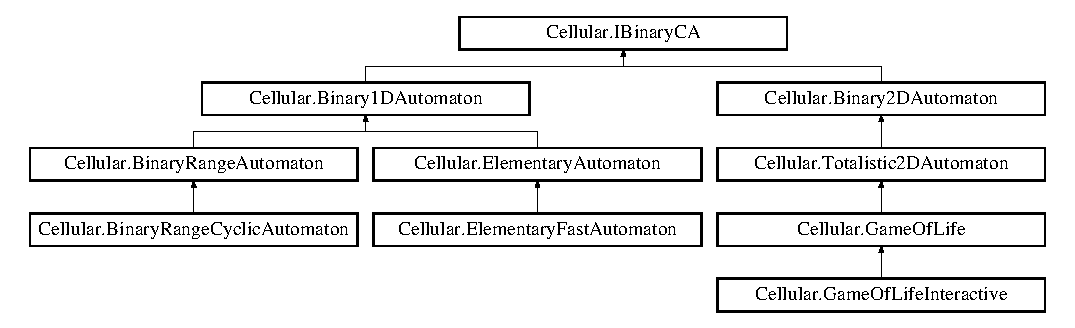
\includegraphics[height=2.974767cm]{interface_cellular_1_1_i_binary_c_a}
\end{center}
\end{figure}
\subsection*{Public Member Functions}
\begin{DoxyCompactItemize}
\item 
int \hyperlink{interface_cellular_1_1_i_binary_c_a_ae9a650d8dac5a23ebb051b00e2dc3dee}{Get\+Size} ()
\begin{DoxyCompactList}\small\item\em Tells the size of the C\+A. \end{DoxyCompactList}\item 
string \hyperlink{interface_cellular_1_1_i_binary_c_a_ab70ebcefac0ca22dd06661f3316a6c2e}{State\+As\+String} ()
\begin{DoxyCompactList}\small\item\em Converts the inner state of the C\+A into a well-\/printable string using \end{DoxyCompactList}\item 
uint\mbox{[}$\,$\mbox{]} \hyperlink{interface_cellular_1_1_i_binary_c_a_a62f943d92c7aedd121f99940ff12c63e}{Get\+Packed} ()
\begin{DoxyCompactList}\small\item\em Converts the inner state of the C\+A into an array of {\ttfamily System.\+U\+Int32}. So every 32 cells are saved into one uint (where the original array is treated as M\+S\+B-\/first). \end{DoxyCompactList}\item 
bool \hyperlink{interface_cellular_1_1_i_binary_c_a_a809b66186b663b64d85db59237693b52}{Get\+Value\+At} (int index)
\begin{DoxyCompactList}\small\item\em Tells the specified bit of the C\+A. \end{DoxyCompactList}\item 
void \hyperlink{interface_cellular_1_1_i_binary_c_a_a6a04c7374538c49df07efa176e0dd3c3}{Step} ()
\begin{DoxyCompactList}\small\item\em Performs one step of the cellular automaton. Always calls \end{DoxyCompactList}\item 
\hyperlink{interface_cellular_1_1_i_binary_c_a}{I\+Binary\+C\+A} \hyperlink{interface_cellular_1_1_i_binary_c_a_a0d5610129c1f7aee62d6521ba8268cf9}{Clone\+Everything} ()
\begin{DoxyCompactList}\small\item\em Clones the underlying C\+A including its state at the moment. \end{DoxyCompactList}\item 
\hyperlink{interface_cellular_1_1_i_binary_c_a}{I\+Binary\+C\+A} \hyperlink{interface_cellular_1_1_i_binary_c_a_a1adc2170335c41093d2da999523896ec}{Clone\+Template} (Bit\+Array new\+Instance\+State)
\begin{DoxyCompactList}\small\item\em Creates a new binary C\+A with the same type and the same rules. \end{DoxyCompactList}\item 
string \hyperlink{interface_cellular_1_1_i_binary_c_a_aa67feabf5d1513aa74076d255c661948}{Tell\+Type} ()
\begin{DoxyCompactList}\small\item\em Announces the runtime type of the C\+A including info about its rule. It serves for debugging purposes. \end{DoxyCompactList}\end{DoxyCompactItemize}


\subsection{Detailed Description}
Common interface for all binary cellular automata. Most work with C\+A is done through this interface. Only subclasses of {\ttfamily \hyperlink{class_cellular_1_1_cellular_automaton}{Cellular\+Automaton}} are supposed to implement this interface. 



Definition at line 9 of file I\+Binary\+C\+A.\+cs.



\subsection{Member Function Documentation}
\hypertarget{interface_cellular_1_1_i_binary_c_a_a0d5610129c1f7aee62d6521ba8268cf9}{}\index{Cellular\+::\+I\+Binary\+C\+A@{Cellular\+::\+I\+Binary\+C\+A}!Clone\+Everything@{Clone\+Everything}}
\index{Clone\+Everything@{Clone\+Everything}!Cellular\+::\+I\+Binary\+C\+A@{Cellular\+::\+I\+Binary\+C\+A}}
\subsubsection[{Clone\+Everything()}]{\setlength{\rightskip}{0pt plus 5cm}{\bf I\+Binary\+C\+A} Cellular.\+I\+Binary\+C\+A.\+Clone\+Everything (
\begin{DoxyParamCaption}
{}
\end{DoxyParamCaption}
)}\label{interface_cellular_1_1_i_binary_c_a_a0d5610129c1f7aee62d6521ba8268cf9}


Clones the underlying C\+A including its state at the moment. 

\begin{DoxyReturn}{Returns}
Identical copy. The result is the same as when calling 
\begin{DoxyCode}
CellularAutomaton.Clone();
\end{DoxyCode}
, only its type is {\ttfamily \hyperlink{interface_cellular_1_1_i_binary_c_a}{I\+Binary\+C\+A}} (which is useful).
\end{DoxyReturn}
\hypertarget{interface_cellular_1_1_i_binary_c_a_a1adc2170335c41093d2da999523896ec}{}\index{Cellular\+::\+I\+Binary\+C\+A@{Cellular\+::\+I\+Binary\+C\+A}!Clone\+Template@{Clone\+Template}}
\index{Clone\+Template@{Clone\+Template}!Cellular\+::\+I\+Binary\+C\+A@{Cellular\+::\+I\+Binary\+C\+A}}
\subsubsection[{Clone\+Template(\+Bit\+Array new\+Instance\+State)}]{\setlength{\rightskip}{0pt plus 5cm}{\bf I\+Binary\+C\+A} Cellular.\+I\+Binary\+C\+A.\+Clone\+Template (
\begin{DoxyParamCaption}
\item[{Bit\+Array}]{new\+Instance\+State}
\end{DoxyParamCaption}
)}\label{interface_cellular_1_1_i_binary_c_a_a1adc2170335c41093d2da999523896ec}


Creates a new binary C\+A with the same type and the same rules. 


\begin{DoxyParams}{Parameters}
{\em new\+Instance\+State} & Initial state of the new (returned) instance.\\
\hline
\end{DoxyParams}
\begin{DoxyReturn}{Returns}
New binary C\+A with identical behaviour, but newly given initial state.
\end{DoxyReturn}
\hypertarget{interface_cellular_1_1_i_binary_c_a_a62f943d92c7aedd121f99940ff12c63e}{}\index{Cellular\+::\+I\+Binary\+C\+A@{Cellular\+::\+I\+Binary\+C\+A}!Get\+Packed@{Get\+Packed}}
\index{Get\+Packed@{Get\+Packed}!Cellular\+::\+I\+Binary\+C\+A@{Cellular\+::\+I\+Binary\+C\+A}}
\subsubsection[{Get\+Packed()}]{\setlength{\rightskip}{0pt plus 5cm}uint \mbox{[}$\,$\mbox{]} Cellular.\+I\+Binary\+C\+A.\+Get\+Packed (
\begin{DoxyParamCaption}
{}
\end{DoxyParamCaption}
)}\label{interface_cellular_1_1_i_binary_c_a_a62f943d92c7aedd121f99940ff12c63e}


Converts the inner state of the C\+A into an array of {\ttfamily System.\+U\+Int32}. So every 32 cells are saved into one uint (where the original array is treated as M\+S\+B-\/first). 

\begin{DoxyReturn}{Returns}
Condensed state of the C\+A.
\end{DoxyReturn}
\hypertarget{interface_cellular_1_1_i_binary_c_a_ae9a650d8dac5a23ebb051b00e2dc3dee}{}\index{Cellular\+::\+I\+Binary\+C\+A@{Cellular\+::\+I\+Binary\+C\+A}!Get\+Size@{Get\+Size}}
\index{Get\+Size@{Get\+Size}!Cellular\+::\+I\+Binary\+C\+A@{Cellular\+::\+I\+Binary\+C\+A}}
\subsubsection[{Get\+Size()}]{\setlength{\rightskip}{0pt plus 5cm}int Cellular.\+I\+Binary\+C\+A.\+Get\+Size (
\begin{DoxyParamCaption}
{}
\end{DoxyParamCaption}
)}\label{interface_cellular_1_1_i_binary_c_a_ae9a650d8dac5a23ebb051b00e2dc3dee}


Tells the size of the C\+A. 

\begin{DoxyReturn}{Returns}
Number of cells/bits.
\end{DoxyReturn}
\hypertarget{interface_cellular_1_1_i_binary_c_a_a809b66186b663b64d85db59237693b52}{}\index{Cellular\+::\+I\+Binary\+C\+A@{Cellular\+::\+I\+Binary\+C\+A}!Get\+Value\+At@{Get\+Value\+At}}
\index{Get\+Value\+At@{Get\+Value\+At}!Cellular\+::\+I\+Binary\+C\+A@{Cellular\+::\+I\+Binary\+C\+A}}
\subsubsection[{Get\+Value\+At(int index)}]{\setlength{\rightskip}{0pt plus 5cm}bool Cellular.\+I\+Binary\+C\+A.\+Get\+Value\+At (
\begin{DoxyParamCaption}
\item[{int}]{index}
\end{DoxyParamCaption}
)}\label{interface_cellular_1_1_i_binary_c_a_a809b66186b663b64d85db59237693b52}


Tells the specified bit of the C\+A. 


\begin{DoxyParams}{Parameters}
{\em index} & Zero-\/based index (which bit is required).\\
\hline
\end{DoxyParams}
\begin{DoxyReturn}{Returns}
One bit.
\end{DoxyReturn}
Throws exception if index is out of range.\hypertarget{interface_cellular_1_1_i_binary_c_a_ab70ebcefac0ca22dd06661f3316a6c2e}{}\index{Cellular\+::\+I\+Binary\+C\+A@{Cellular\+::\+I\+Binary\+C\+A}!State\+As\+String@{State\+As\+String}}
\index{State\+As\+String@{State\+As\+String}!Cellular\+::\+I\+Binary\+C\+A@{Cellular\+::\+I\+Binary\+C\+A}}
\subsubsection[{State\+As\+String()}]{\setlength{\rightskip}{0pt plus 5cm}string Cellular.\+I\+Binary\+C\+A.\+State\+As\+String (
\begin{DoxyParamCaption}
{}
\end{DoxyParamCaption}
)}\label{interface_cellular_1_1_i_binary_c_a_ab70ebcefac0ca22dd06661f3316a6c2e}


Converts the inner state of the C\+A into a well-\/printable string using 

{\ttfamily state\mbox{[}i\mbox{]} ? \textquotesingle{}█\textquotesingle{} \+: \textquotesingle{} \textquotesingle{};} 

\begin{DoxyReturn}{Returns}
State of the C\+A as a string.
\end{DoxyReturn}
\hypertarget{interface_cellular_1_1_i_binary_c_a_a6a04c7374538c49df07efa176e0dd3c3}{}\index{Cellular\+::\+I\+Binary\+C\+A@{Cellular\+::\+I\+Binary\+C\+A}!Step@{Step}}
\index{Step@{Step}!Cellular\+::\+I\+Binary\+C\+A@{Cellular\+::\+I\+Binary\+C\+A}}
\subsubsection[{Step()}]{\setlength{\rightskip}{0pt plus 5cm}void Cellular.\+I\+Binary\+C\+A.\+Step (
\begin{DoxyParamCaption}
{}
\end{DoxyParamCaption}
)}\label{interface_cellular_1_1_i_binary_c_a_a6a04c7374538c49df07efa176e0dd3c3}


Performs one step of the cellular automaton. Always calls 

{\ttfamily \hyperlink{class_cellular_1_1_cellular_automaton_aa70848d58015575974bc875ac5a89ae7}{Cellular\+Automaton.\+Step()};}. 

Implemented in \hyperlink{class_cellular_1_1_totalistic2_d_automaton_a7f85cac5420f67a936cbd4cef33c4abc}{Cellular.\+Totalistic2\+D\+Automaton}, \hyperlink{class_cellular_1_1_elementary_automaton_adae7c322e4c7cd00cd0534a23d1abfa4}{Cellular.\+Elementary\+Automaton}, \hyperlink{class_cellular_1_1_binary_range_automaton_ade1f5b831b9676f04f835c33d245b9e2}{Cellular.\+Binary\+Range\+Automaton}, and \hyperlink{class_cellular_1_1_elementary_fast_automaton_aa877bef8b8242c58e190a884d18f3b5f}{Cellular.\+Elementary\+Fast\+Automaton}.

\hypertarget{interface_cellular_1_1_i_binary_c_a_aa67feabf5d1513aa74076d255c661948}{}\index{Cellular\+::\+I\+Binary\+C\+A@{Cellular\+::\+I\+Binary\+C\+A}!Tell\+Type@{Tell\+Type}}
\index{Tell\+Type@{Tell\+Type}!Cellular\+::\+I\+Binary\+C\+A@{Cellular\+::\+I\+Binary\+C\+A}}
\subsubsection[{Tell\+Type()}]{\setlength{\rightskip}{0pt plus 5cm}string Cellular.\+I\+Binary\+C\+A.\+Tell\+Type (
\begin{DoxyParamCaption}
{}
\end{DoxyParamCaption}
)}\label{interface_cellular_1_1_i_binary_c_a_aa67feabf5d1513aa74076d255c661948}


Announces the runtime type of the C\+A including info about its rule. It serves for debugging purposes. 

\begin{DoxyReturn}{Returns}
The same string as calling 
\begin{DoxyCode}
CellularAutomaton.TellType();
\end{DoxyCode}
.
\end{DoxyReturn}


Implemented in \hyperlink{class_cellular_1_1_totalistic2_d_automaton_aa009c674cd109fa70173e9893f6d3b09}{Cellular.\+Totalistic2\+D\+Automaton}, \hyperlink{class_cellular_1_1_binary_range_automaton_afad205eb4fea51efd63b063f96bfda5c}{Cellular.\+Binary\+Range\+Automaton}, \hyperlink{class_cellular_1_1_elementary_automaton_a812677139d560e2c600226361b785995}{Cellular.\+Elementary\+Automaton}, and \hyperlink{class_cellular_1_1_binary_range_cyclic_automaton_a75754d1c54550e1f29a9282647947cb8}{Cellular.\+Binary\+Range\+Cyclic\+Automaton}.



The documentation for this interface was generated from the following file\+:\begin{DoxyCompactItemize}
\item 
C\+:/\+Martin/\+M\+F\+F/\+\_\+baka/\+Martin\+Dvorak/\+Cellular/\hyperlink{_i_binary_c_a_8cs}{I\+Binary\+C\+A.\+cs}\end{DoxyCompactItemize}

\input{interface_crypto_1_1_i_encrypter}
\hypertarget{interface_crypto_1_1_i_key_extender}{}\section{Crypto.\+I\+Key\+Extender Interface Reference}
\label{interface_crypto_1_1_i_key_extender}\index{Crypto.\+I\+Key\+Extender@{Crypto.\+I\+Key\+Extender}}


Interface for all algorithms that can perform key stretching. Can be used from any assembly.  


Inheritance diagram for Crypto.\+I\+Key\+Extender\+:\begin{figure}[H]
\begin{center}
\leavevmode
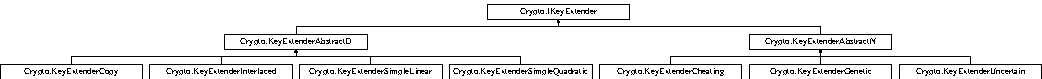
\includegraphics[height=1.057269cm]{interface_crypto_1_1_i_key_extender}
\end{center}
\end{figure}
\subsection*{Public Member Functions}
\begin{DoxyCompactItemize}
\item 
Bit\+Array \hyperlink{interface_crypto_1_1_i_key_extender_a946f0bf735d90050a4ba5335ca920fd1}{Double\+Key} (Bit\+Array short\+Key)
\begin{DoxyCompactList}\small\item\em Generates a longer key from a short key. \end{DoxyCompactList}\item 
Bit\+Array \hyperlink{interface_crypto_1_1_i_key_extender_a0412d4d5b8d41546f9d6d126d3b4519f}{Extend\+Key} (Bit\+Array short\+Key, int target\+Length)
\begin{DoxyCompactList}\small\item\em Generates a longer key from a short key. \end{DoxyCompactList}\end{DoxyCompactItemize}


\subsection{Detailed Description}
Interface for all algorithms that can perform key stretching. Can be used from any assembly. 



Definition at line 8 of file I\+Key\+Extender.\+cs.



\subsection{Member Function Documentation}
\hypertarget{interface_crypto_1_1_i_key_extender_a946f0bf735d90050a4ba5335ca920fd1}{}\index{Crypto\+::\+I\+Key\+Extender@{Crypto\+::\+I\+Key\+Extender}!Double\+Key@{Double\+Key}}
\index{Double\+Key@{Double\+Key}!Crypto\+::\+I\+Key\+Extender@{Crypto\+::\+I\+Key\+Extender}}
\subsubsection[{Double\+Key(\+Bit\+Array short\+Key)}]{\setlength{\rightskip}{0pt plus 5cm}Bit\+Array Crypto.\+I\+Key\+Extender.\+Double\+Key (
\begin{DoxyParamCaption}
\item[{Bit\+Array}]{short\+Key}
\end{DoxyParamCaption}
)}\label{interface_crypto_1_1_i_key_extender_a946f0bf735d90050a4ba5335ca920fd1}


Generates a longer key from a short key. 


\begin{DoxyParams}{Parameters}
{\em short\+Key} & Short key to be stretched (doubled).\\
\hline
\end{DoxyParams}
\begin{DoxyReturn}{Returns}
Long key (twice longer than input).
\end{DoxyReturn}


Implemented in \hyperlink{class_crypto_1_1_key_extender_interlaced_a1caf1b3ad04b24305f964ab44a399751}{Crypto.\+Key\+Extender\+Interlaced}, \hyperlink{class_crypto_1_1_key_extender_simple_quadratic_a0bba7646011678850879c0685d18b379}{Crypto.\+Key\+Extender\+Simple\+Quadratic}, \hyperlink{class_crypto_1_1_key_extender_simple_linear_a1b511ea8a0e0bb6cbd4f6a94f49015bd}{Crypto.\+Key\+Extender\+Simple\+Linear}, \hyperlink{class_crypto_1_1_key_extender_abstract_d_ae403b92e9038b9c0bc7a21885e24ffc7}{Crypto.\+Key\+Extender\+Abstract\+D}, \hyperlink{class_crypto_1_1_key_extender_abstract_n_a57e9a8247ebde9e639c16107c2961d10}{Crypto.\+Key\+Extender\+Abstract\+N}, and \hyperlink{class_crypto_1_1_key_extender_copy_ab57d10f5c80bbf6ab395e0a0b690080a}{Crypto.\+Key\+Extender\+Copy}.

\hypertarget{interface_crypto_1_1_i_key_extender_a0412d4d5b8d41546f9d6d126d3b4519f}{}\index{Crypto\+::\+I\+Key\+Extender@{Crypto\+::\+I\+Key\+Extender}!Extend\+Key@{Extend\+Key}}
\index{Extend\+Key@{Extend\+Key}!Crypto\+::\+I\+Key\+Extender@{Crypto\+::\+I\+Key\+Extender}}
\subsubsection[{Extend\+Key(\+Bit\+Array short\+Key, int target\+Length)}]{\setlength{\rightskip}{0pt plus 5cm}Bit\+Array Crypto.\+I\+Key\+Extender.\+Extend\+Key (
\begin{DoxyParamCaption}
\item[{Bit\+Array}]{short\+Key, }
\item[{int}]{target\+Length}
\end{DoxyParamCaption}
)}\label{interface_crypto_1_1_i_key_extender_a0412d4d5b8d41546f9d6d126d3b4519f}


Generates a longer key from a short key. 


\begin{DoxyParams}{Parameters}
{\em short\+Key} & Short key to be stretched (multiplied).\\
\hline
{\em target\+Length} & How many bits should the resulting long key have?\\
\hline
\end{DoxyParams}
\begin{DoxyReturn}{Returns}
Long key (of specified length).
\end{DoxyReturn}


Implemented in \hyperlink{class_crypto_1_1_key_extender_uncertain_a2955df98d2f4831576b12aa9c5ec609d}{Crypto.\+Key\+Extender\+Uncertain}, \hyperlink{class_crypto_1_1_key_extender_abstract_n_a9df4156ad0a84730f87119e5a25cf1ef}{Crypto.\+Key\+Extender\+Abstract\+N}, \hyperlink{class_crypto_1_1_key_extender_abstract_d_a3ec7fa96f391d840043eff0c8409d130}{Crypto.\+Key\+Extender\+Abstract\+D}, and \hyperlink{class_crypto_1_1_key_extender_cheating_a8018900fc6f660f83cb7cd23d52b60a3}{Crypto.\+Key\+Extender\+Cheating}.



The documentation for this interface was generated from the following file\+:\begin{DoxyCompactItemize}
\item 
C\+:/\+Martin/\+M\+F\+F/\+\_\+baka/\+Martin\+Dvorak/\+Crypto/\hyperlink{_i_key_extender_8cs}{I\+Key\+Extender.\+cs}\end{DoxyCompactItemize}

\hypertarget{class_crypto_1_1_key_extender_abstract_d}{}\section{Crypto.\+Key\+Extender\+Abstract\+D Class Reference}
\label{class_crypto_1_1_key_extender_abstract_d}\index{Crypto.\+Key\+Extender\+Abstract\+D@{Crypto.\+Key\+Extender\+Abstract\+D}}


Abstract class for all key extenders that implement \hyperlink{class_crypto_1_1_key_extender_abstract_d_ae403b92e9038b9c0bc7a21885e24ffc7}{Double\+Key()}. Method \hyperlink{class_crypto_1_1_key_extender_abstract_d_a3ec7fa96f391d840043eff0c8409d130}{Extend\+Key()} is provided (iterates \hyperlink{class_crypto_1_1_key_extender_abstract_d_ae403b92e9038b9c0bc7a21885e24ffc7}{Double\+Key()} method until we get a desired length).  


Inheritance diagram for Crypto.\+Key\+Extender\+Abstract\+D\+:\begin{figure}[H]
\begin{center}
\leavevmode
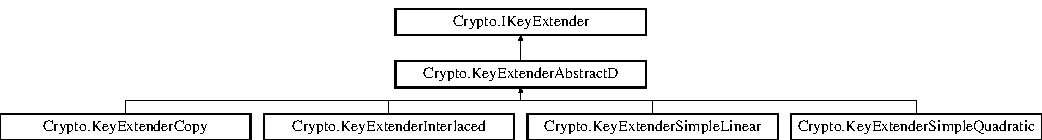
\includegraphics[height=1.850220cm]{class_crypto_1_1_key_extender_abstract_d}
\end{center}
\end{figure}
\subsection*{Public Member Functions}
\begin{DoxyCompactItemize}
\item 
abstract Bit\+Array \hyperlink{class_crypto_1_1_key_extender_abstract_d_ae403b92e9038b9c0bc7a21885e24ffc7}{Double\+Key} (Bit\+Array short\+Key)
\begin{DoxyCompactList}\small\item\em Generates a longer key from a short key. \end{DoxyCompactList}\item 
Bit\+Array \hyperlink{class_crypto_1_1_key_extender_abstract_d_a3ec7fa96f391d840043eff0c8409d130}{Extend\+Key} (Bit\+Array short\+Key, int target\+Length)
\begin{DoxyCompactList}\small\item\em Generates a longer key from a short key. \end{DoxyCompactList}\end{DoxyCompactItemize}


\subsection{Detailed Description}
Abstract class for all key extenders that implement \hyperlink{class_crypto_1_1_key_extender_abstract_d_ae403b92e9038b9c0bc7a21885e24ffc7}{Double\+Key()}. Method \hyperlink{class_crypto_1_1_key_extender_abstract_d_a3ec7fa96f391d840043eff0c8409d130}{Extend\+Key()} is provided (iterates \hyperlink{class_crypto_1_1_key_extender_abstract_d_ae403b92e9038b9c0bc7a21885e24ffc7}{Double\+Key()} method until we get a desired length). 



Definition at line 9 of file Key\+Extender\+Abstract\+D.\+cs.



\subsection{Member Function Documentation}
\hypertarget{class_crypto_1_1_key_extender_abstract_d_ae403b92e9038b9c0bc7a21885e24ffc7}{}\index{Crypto\+::\+Key\+Extender\+Abstract\+D@{Crypto\+::\+Key\+Extender\+Abstract\+D}!Double\+Key@{Double\+Key}}
\index{Double\+Key@{Double\+Key}!Crypto\+::\+Key\+Extender\+Abstract\+D@{Crypto\+::\+Key\+Extender\+Abstract\+D}}
\subsubsection[{Double\+Key(\+Bit\+Array short\+Key)}]{\setlength{\rightskip}{0pt plus 5cm}abstract Bit\+Array Crypto.\+Key\+Extender\+Abstract\+D.\+Double\+Key (
\begin{DoxyParamCaption}
\item[{Bit\+Array}]{short\+Key}
\end{DoxyParamCaption}
)\hspace{0.3cm}{\ttfamily [pure virtual]}}\label{class_crypto_1_1_key_extender_abstract_d_ae403b92e9038b9c0bc7a21885e24ffc7}


Generates a longer key from a short key. 


\begin{DoxyParams}{Parameters}
{\em short\+Key} & Short key to be stretched (doubled).\\
\hline
\end{DoxyParams}
\begin{DoxyReturn}{Returns}
Long key (twice longer than input).
\end{DoxyReturn}


Implements \hyperlink{interface_crypto_1_1_i_key_extender_a946f0bf735d90050a4ba5335ca920fd1}{Crypto.\+I\+Key\+Extender}.



Implemented in \hyperlink{class_crypto_1_1_key_extender_interlaced_a1caf1b3ad04b24305f964ab44a399751}{Crypto.\+Key\+Extender\+Interlaced}, \hyperlink{class_crypto_1_1_key_extender_simple_quadratic_a0bba7646011678850879c0685d18b379}{Crypto.\+Key\+Extender\+Simple\+Quadratic}, \hyperlink{class_crypto_1_1_key_extender_simple_linear_a1b511ea8a0e0bb6cbd4f6a94f49015bd}{Crypto.\+Key\+Extender\+Simple\+Linear}, and \hyperlink{class_crypto_1_1_key_extender_copy_ab57d10f5c80bbf6ab395e0a0b690080a}{Crypto.\+Key\+Extender\+Copy}.

\hypertarget{class_crypto_1_1_key_extender_abstract_d_a3ec7fa96f391d840043eff0c8409d130}{}\index{Crypto\+::\+Key\+Extender\+Abstract\+D@{Crypto\+::\+Key\+Extender\+Abstract\+D}!Extend\+Key@{Extend\+Key}}
\index{Extend\+Key@{Extend\+Key}!Crypto\+::\+Key\+Extender\+Abstract\+D@{Crypto\+::\+Key\+Extender\+Abstract\+D}}
\subsubsection[{Extend\+Key(\+Bit\+Array short\+Key, int target\+Length)}]{\setlength{\rightskip}{0pt plus 5cm}Bit\+Array Crypto.\+Key\+Extender\+Abstract\+D.\+Extend\+Key (
\begin{DoxyParamCaption}
\item[{Bit\+Array}]{short\+Key, }
\item[{int}]{target\+Length}
\end{DoxyParamCaption}
)}\label{class_crypto_1_1_key_extender_abstract_d_a3ec7fa96f391d840043eff0c8409d130}


Generates a longer key from a short key. 


\begin{DoxyParams}{Parameters}
{\em short\+Key} & Short key to be stretched (multiplied).\\
\hline
{\em target\+Length} & How many bits should the resulting long key have?\\
\hline
\end{DoxyParams}
\begin{DoxyReturn}{Returns}
Long key (of specified length).
\end{DoxyReturn}


Implements \hyperlink{interface_crypto_1_1_i_key_extender_a0412d4d5b8d41546f9d6d126d3b4519f}{Crypto.\+I\+Key\+Extender}.



Definition at line 13 of file Key\+Extender\+Abstract\+D.\+cs.



The documentation for this class was generated from the following file\+:\begin{DoxyCompactItemize}
\item 
C\+:/\+Martin/\+M\+F\+F/\+\_\+baka/\+Martin\+Dvorak/\+Crypto/\hyperlink{_key_extender_abstract_d_8cs}{Key\+Extender\+Abstract\+D.\+cs}\end{DoxyCompactItemize}

\hypertarget{class_crypto_1_1_key_extender_abstract_n}{}\section{Crypto.\+Key\+Extender\+Abstract\+N Class Reference}
\label{class_crypto_1_1_key_extender_abstract_n}\index{Crypto.\+Key\+Extender\+Abstract\+N@{Crypto.\+Key\+Extender\+Abstract\+N}}


Abstract class for all key extenders that implement \hyperlink{class_crypto_1_1_key_extender_abstract_n_a9df4156ad0a84730f87119e5a25cf1ef}{Extend\+Key()}. Method \hyperlink{class_crypto_1_1_key_extender_abstract_n_a57e9a8247ebde9e639c16107c2961d10}{Double\+Key()} simply calls \hyperlink{class_crypto_1_1_key_extender_abstract_n_a9df4156ad0a84730f87119e5a25cf1ef}{Extend\+Key()}.  


Inheritance diagram for Crypto.\+Key\+Extender\+Abstract\+N\+:\begin{figure}[H]
\begin{center}
\leavevmode
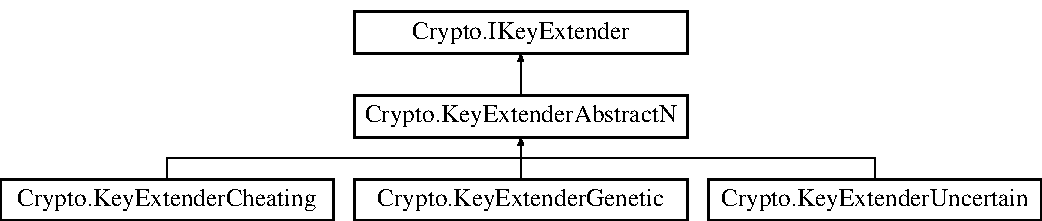
\includegraphics[height=2.947368cm]{class_crypto_1_1_key_extender_abstract_n}
\end{center}
\end{figure}
\subsection*{Public Member Functions}
\begin{DoxyCompactItemize}
\item 
Bit\+Array \hyperlink{class_crypto_1_1_key_extender_abstract_n_a57e9a8247ebde9e639c16107c2961d10}{Double\+Key} (Bit\+Array short\+Key)
\begin{DoxyCompactList}\small\item\em Generates a longer key from a short key. \end{DoxyCompactList}\item 
abstract Bit\+Array \hyperlink{class_crypto_1_1_key_extender_abstract_n_a9df4156ad0a84730f87119e5a25cf1ef}{Extend\+Key} (Bit\+Array short\+Key, int target\+Length)
\begin{DoxyCompactList}\small\item\em Generates a longer key from a short key. \end{DoxyCompactList}\end{DoxyCompactItemize}


\subsection{Detailed Description}
Abstract class for all key extenders that implement \hyperlink{class_crypto_1_1_key_extender_abstract_n_a9df4156ad0a84730f87119e5a25cf1ef}{Extend\+Key()}. Method \hyperlink{class_crypto_1_1_key_extender_abstract_n_a57e9a8247ebde9e639c16107c2961d10}{Double\+Key()} simply calls \hyperlink{class_crypto_1_1_key_extender_abstract_n_a9df4156ad0a84730f87119e5a25cf1ef}{Extend\+Key()}. 



Definition at line 8 of file Key\+Extender\+Abstract\+N.\+cs.



\subsection{Member Function Documentation}
\hypertarget{class_crypto_1_1_key_extender_abstract_n_a57e9a8247ebde9e639c16107c2961d10}{}\index{Crypto\+::\+Key\+Extender\+Abstract\+N@{Crypto\+::\+Key\+Extender\+Abstract\+N}!Double\+Key@{Double\+Key}}
\index{Double\+Key@{Double\+Key}!Crypto\+::\+Key\+Extender\+Abstract\+N@{Crypto\+::\+Key\+Extender\+Abstract\+N}}
\subsubsection[{Double\+Key(\+Bit\+Array short\+Key)}]{\setlength{\rightskip}{0pt plus 5cm}Bit\+Array Crypto.\+Key\+Extender\+Abstract\+N.\+Double\+Key (
\begin{DoxyParamCaption}
\item[{Bit\+Array}]{short\+Key}
\end{DoxyParamCaption}
)}\label{class_crypto_1_1_key_extender_abstract_n_a57e9a8247ebde9e639c16107c2961d10}


Generates a longer key from a short key. 


\begin{DoxyParams}{Parameters}
{\em short\+Key} & Short key to be stretched (doubled).\\
\hline
\end{DoxyParams}
\begin{DoxyReturn}{Returns}
Long key (twice longer than input).
\end{DoxyReturn}


Implements \hyperlink{interface_crypto_1_1_i_key_extender_a946f0bf735d90050a4ba5335ca920fd1}{Crypto.\+I\+Key\+Extender}.



Definition at line 10 of file Key\+Extender\+Abstract\+N.\+cs.

\hypertarget{class_crypto_1_1_key_extender_abstract_n_a9df4156ad0a84730f87119e5a25cf1ef}{}\index{Crypto\+::\+Key\+Extender\+Abstract\+N@{Crypto\+::\+Key\+Extender\+Abstract\+N}!Extend\+Key@{Extend\+Key}}
\index{Extend\+Key@{Extend\+Key}!Crypto\+::\+Key\+Extender\+Abstract\+N@{Crypto\+::\+Key\+Extender\+Abstract\+N}}
\subsubsection[{Extend\+Key(\+Bit\+Array short\+Key, int target\+Length)}]{\setlength{\rightskip}{0pt plus 5cm}abstract Bit\+Array Crypto.\+Key\+Extender\+Abstract\+N.\+Extend\+Key (
\begin{DoxyParamCaption}
\item[{Bit\+Array}]{short\+Key, }
\item[{int}]{target\+Length}
\end{DoxyParamCaption}
)\hspace{0.3cm}{\ttfamily [pure virtual]}}\label{class_crypto_1_1_key_extender_abstract_n_a9df4156ad0a84730f87119e5a25cf1ef}


Generates a longer key from a short key. 


\begin{DoxyParams}{Parameters}
{\em short\+Key} & Short key to be stretched (multiplied).\\
\hline
{\em target\+Length} & How many bits should the resulting long key have?\\
\hline
\end{DoxyParams}
\begin{DoxyReturn}{Returns}
Long key (of specified length).
\end{DoxyReturn}


Implements \hyperlink{interface_crypto_1_1_i_key_extender_a0412d4d5b8d41546f9d6d126d3b4519f}{Crypto.\+I\+Key\+Extender}.



Implemented in \hyperlink{class_crypto_1_1_key_extender_uncertain_a2955df98d2f4831576b12aa9c5ec609d}{Crypto.\+Key\+Extender\+Uncertain}, and \hyperlink{class_crypto_1_1_key_extender_cheating_a8018900fc6f660f83cb7cd23d52b60a3}{Crypto.\+Key\+Extender\+Cheating}.



The documentation for this class was generated from the following file\+:\begin{DoxyCompactItemize}
\item 
C\+:/\+Martin/\+M\+F\+F/\+\_\+baka/\+Martin\+Dvorak/\+Crypto/\hyperlink{_key_extender_abstract_n_8cs}{Key\+Extender\+Abstract\+N.\+cs}\end{DoxyCompactItemize}

\hypertarget{class_crypto_1_1_key_extender_cheating}{}\section{Crypto.\+Key\+Extender\+Cheating Class Reference}
\label{class_crypto_1_1_key_extender_cheating}\index{Crypto.\+Key\+Extender\+Cheating@{Crypto.\+Key\+Extender\+Cheating}}


Fake key extender which only generates random long key independently of the short key.  


Inheritance diagram for Crypto.\+Key\+Extender\+Cheating\+:\begin{figure}[H]
\begin{center}
\leavevmode
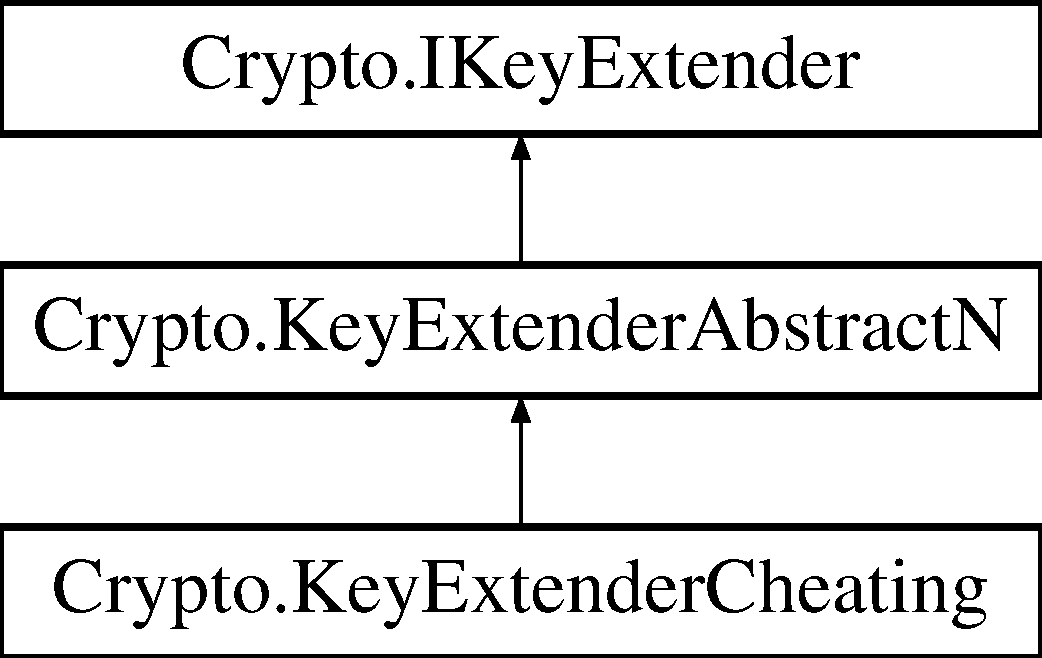
\includegraphics[height=3.000000cm]{class_crypto_1_1_key_extender_cheating}
\end{center}
\end{figure}
\subsection*{Public Member Functions}
\begin{DoxyCompactItemize}
\item 
override Bit\+Array \hyperlink{class_crypto_1_1_key_extender_cheating_a8018900fc6f660f83cb7cd23d52b60a3}{Extend\+Key} (Bit\+Array short\+Key, int target\+Length)
\begin{DoxyCompactList}\small\item\em Generates a longer key from a short key. \end{DoxyCompactList}\end{DoxyCompactItemize}


\subsection{Detailed Description}
Fake key extender which only generates random long key independently of the short key. 



Definition at line 9 of file Key\+Extender\+Cheating.\+cs.



\subsection{Member Function Documentation}
\hypertarget{class_crypto_1_1_key_extender_cheating_a8018900fc6f660f83cb7cd23d52b60a3}{}\index{Crypto\+::\+Key\+Extender\+Cheating@{Crypto\+::\+Key\+Extender\+Cheating}!Extend\+Key@{Extend\+Key}}
\index{Extend\+Key@{Extend\+Key}!Crypto\+::\+Key\+Extender\+Cheating@{Crypto\+::\+Key\+Extender\+Cheating}}
\subsubsection[{Extend\+Key(\+Bit\+Array short\+Key, int target\+Length)}]{\setlength{\rightskip}{0pt plus 5cm}override Bit\+Array Crypto.\+Key\+Extender\+Cheating.\+Extend\+Key (
\begin{DoxyParamCaption}
\item[{Bit\+Array}]{short\+Key, }
\item[{int}]{target\+Length}
\end{DoxyParamCaption}
)\hspace{0.3cm}{\ttfamily [virtual]}}\label{class_crypto_1_1_key_extender_cheating_a8018900fc6f660f83cb7cd23d52b60a3}


Generates a longer key from a short key. 


\begin{DoxyParams}{Parameters}
{\em short\+Key} & Short key to be stretched (multiplied).\\
\hline
{\em target\+Length} & How many bits should the resulting long key have?\\
\hline
\end{DoxyParams}
\begin{DoxyReturn}{Returns}
Long key (of specified length).
\end{DoxyReturn}


Implements \hyperlink{class_crypto_1_1_key_extender_abstract_n_a9df4156ad0a84730f87119e5a25cf1ef}{Crypto.\+Key\+Extender\+Abstract\+N}.



Definition at line 11 of file Key\+Extender\+Cheating.\+cs.



The documentation for this class was generated from the following file\+:\begin{DoxyCompactItemize}
\item 
C\+:/\+Martin/\+M\+F\+F/\+\_\+baka/\+Martin\+Dvorak/\+Crypto/\hyperlink{_key_extender_cheating_8cs}{Key\+Extender\+Cheating.\+cs}\end{DoxyCompactItemize}

\hypertarget{class_crypto_1_1_key_extender_copy}{}\section{Crypto.\+Key\+Extender\+Copy Class Reference}
\label{class_crypto_1_1_key_extender_copy}\index{Crypto.\+Key\+Extender\+Copy@{Crypto.\+Key\+Extender\+Copy}}


Stupid key extender which only copies the input (repeatedly).  


Inheritance diagram for Crypto.\+Key\+Extender\+Copy\+:\begin{figure}[H]
\begin{center}
\leavevmode
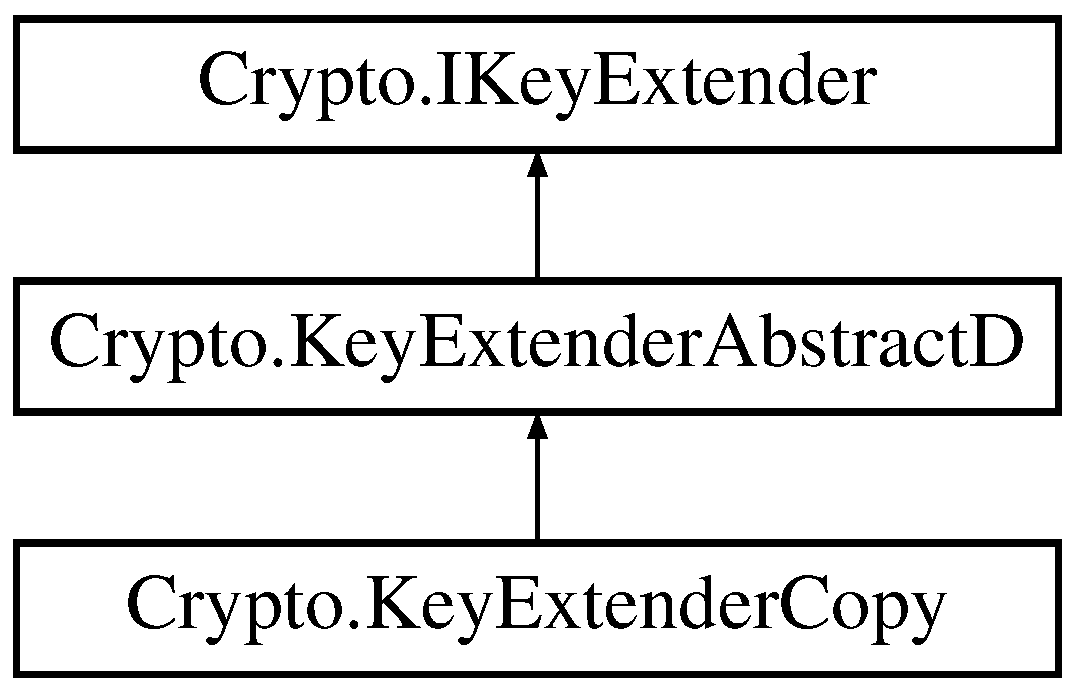
\includegraphics[height=3.000000cm]{class_crypto_1_1_key_extender_copy}
\end{center}
\end{figure}
\subsection*{Public Member Functions}
\begin{DoxyCompactItemize}
\item 
override Bit\+Array \hyperlink{class_crypto_1_1_key_extender_copy_ab57d10f5c80bbf6ab395e0a0b690080a}{Double\+Key} (Bit\+Array short\+Key)
\begin{DoxyCompactList}\small\item\em Generates a longer key from a short key. \end{DoxyCompactList}\end{DoxyCompactItemize}
\subsection*{Package Functions}
\begin{DoxyCompactItemize}
\item 
override string \hyperlink{class_crypto_1_1_key_extender_copy_ab6904bc5e3596cb7ac2cd7840cf356ef}{Get\+Info} ()
\end{DoxyCompactItemize}


\subsection{Detailed Description}
Stupid key extender which only copies the input (repeatedly). 



Definition at line 8 of file Key\+Extender\+Copy.\+cs.



\subsection{Member Function Documentation}
\hypertarget{class_crypto_1_1_key_extender_copy_ab57d10f5c80bbf6ab395e0a0b690080a}{}\index{Crypto\+::\+Key\+Extender\+Copy@{Crypto\+::\+Key\+Extender\+Copy}!Double\+Key@{Double\+Key}}
\index{Double\+Key@{Double\+Key}!Crypto\+::\+Key\+Extender\+Copy@{Crypto\+::\+Key\+Extender\+Copy}}
\subsubsection[{Double\+Key(\+Bit\+Array short\+Key)}]{\setlength{\rightskip}{0pt plus 5cm}override Bit\+Array Crypto.\+Key\+Extender\+Copy.\+Double\+Key (
\begin{DoxyParamCaption}
\item[{Bit\+Array}]{short\+Key}
\end{DoxyParamCaption}
)\hspace{0.3cm}{\ttfamily [virtual]}}\label{class_crypto_1_1_key_extender_copy_ab57d10f5c80bbf6ab395e0a0b690080a}


Generates a longer key from a short key. 


\begin{DoxyParams}{Parameters}
{\em short\+Key} & Short key to be stretched (doubled).\\
\hline
\end{DoxyParams}
\begin{DoxyReturn}{Returns}
Long key (twice longer than input).
\end{DoxyReturn}


Implements \hyperlink{class_crypto_1_1_key_extender_abstract_d_ae403b92e9038b9c0bc7a21885e24ffc7}{Crypto.\+Key\+Extender\+Abstract\+D}.



Definition at line 10 of file Key\+Extender\+Copy.\+cs.

\hypertarget{class_crypto_1_1_key_extender_copy_ab6904bc5e3596cb7ac2cd7840cf356ef}{}\index{Crypto\+::\+Key\+Extender\+Copy@{Crypto\+::\+Key\+Extender\+Copy}!Get\+Info@{Get\+Info}}
\index{Get\+Info@{Get\+Info}!Crypto\+::\+Key\+Extender\+Copy@{Crypto\+::\+Key\+Extender\+Copy}}
\subsubsection[{Get\+Info()}]{\setlength{\rightskip}{0pt plus 5cm}override string Crypto.\+Key\+Extender\+Copy.\+Get\+Info (
\begin{DoxyParamCaption}
{}
\end{DoxyParamCaption}
)\hspace{0.3cm}{\ttfamily [package]}, {\ttfamily [virtual]}}\label{class_crypto_1_1_key_extender_copy_ab6904bc5e3596cb7ac2cd7840cf356ef}


Implements \hyperlink{class_crypto_1_1_key_extender_abstract_d_a954261bd6f533ad7745beac9ce89dd6e}{Crypto.\+Key\+Extender\+Abstract\+D}.



Definition at line 22 of file Key\+Extender\+Copy.\+cs.



The documentation for this class was generated from the following file\+:\begin{DoxyCompactItemize}
\item 
C\+:/\+Martin/\+M\+F\+F/\+\_\+baka/\+Martin\+Dvorak/\+Crypto/\hyperlink{_key_extender_copy_8cs}{Key\+Extender\+Copy.\+cs}\end{DoxyCompactItemize}

\hypertarget{class_crypto_1_1_key_extender_genetic}{}\section{Crypto.\+Key\+Extender\+Genetic Class Reference}
\label{class_crypto_1_1_key_extender_genetic}\index{Crypto.\+Key\+Extender\+Genetic@{Crypto.\+Key\+Extender\+Genetic}}


Algorithms which runs a genetic algorithm to find the best sequence of extenders for each key. Generating the long key may take a very long time.  


Inheritance diagram for Crypto.\+Key\+Extender\+Genetic\+:\begin{figure}[H]
\begin{center}
\leavevmode
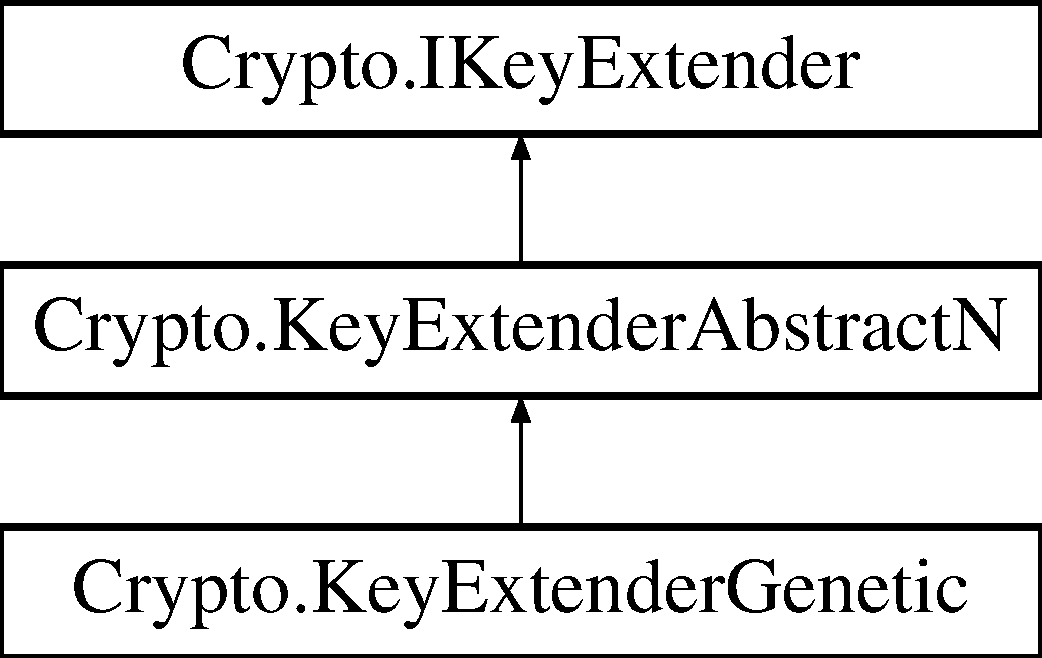
\includegraphics[height=3.000000cm]{class_crypto_1_1_key_extender_genetic}
\end{center}
\end{figure}
\subsection*{Public Member Functions}
\begin{DoxyCompactItemize}
\item 
\hyperlink{class_crypto_1_1_key_extender_genetic_a60bbe95f9ec44c270006a901acf199e5}{Key\+Extender\+Genetic} ()
\end{DoxyCompactItemize}


\subsection{Detailed Description}
Algorithms which runs a genetic algorithm to find the best sequence of extenders for each key. Generating the long key may take a very long time. 



Definition at line 13 of file Key\+Extender\+Genetic.\+cs.



\subsection{Constructor \& Destructor Documentation}
\hypertarget{class_crypto_1_1_key_extender_genetic_a60bbe95f9ec44c270006a901acf199e5}{}\index{Crypto\+::\+Key\+Extender\+Genetic@{Crypto\+::\+Key\+Extender\+Genetic}!Key\+Extender\+Genetic@{Key\+Extender\+Genetic}}
\index{Key\+Extender\+Genetic@{Key\+Extender\+Genetic}!Crypto\+::\+Key\+Extender\+Genetic@{Crypto\+::\+Key\+Extender\+Genetic}}
\subsubsection[{Key\+Extender\+Genetic()}]{\setlength{\rightskip}{0pt plus 5cm}Crypto.\+Key\+Extender\+Genetic.\+Key\+Extender\+Genetic (
\begin{DoxyParamCaption}
{}
\end{DoxyParamCaption}
)}\label{class_crypto_1_1_key_extender_genetic_a60bbe95f9ec44c270006a901acf199e5}


Definition at line 63 of file Key\+Extender\+Genetic.\+cs.



The documentation for this class was generated from the following file\+:\begin{DoxyCompactItemize}
\item 
C\+:/\+Martin/\+M\+F\+F/\+\_\+baka/\+Martin\+Dvorak/\+Crypto/\hyperlink{_key_extender_genetic_8cs}{Key\+Extender\+Genetic.\+cs}\end{DoxyCompactItemize}

\hypertarget{class_crypto_1_1_key_extender_interlaced}{}\section{Crypto.\+Key\+Extender\+Interlaced Class Reference}
\label{class_crypto_1_1_key_extender_interlaced}\index{Crypto.\+Key\+Extender\+Interlaced@{Crypto.\+Key\+Extender\+Interlaced}}


Different linear algorithm, which uses specified number of steps of the underlying C\+A.  


Inheritance diagram for Crypto.\+Key\+Extender\+Interlaced\+:\begin{figure}[H]
\begin{center}
\leavevmode
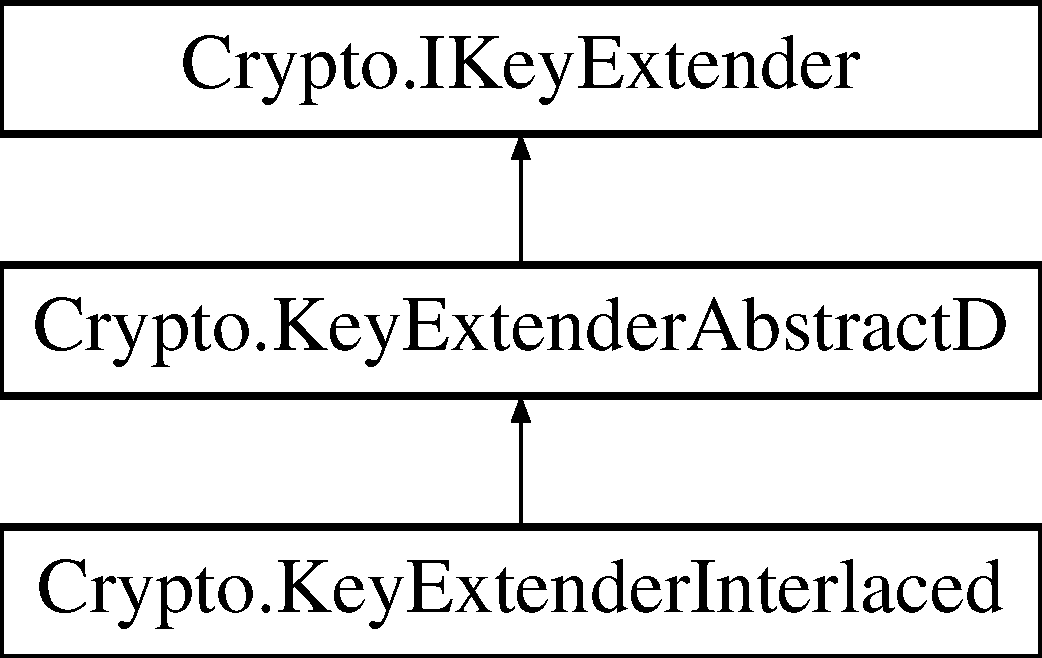
\includegraphics[height=3.000000cm]{class_crypto_1_1_key_extender_interlaced}
\end{center}
\end{figure}
\subsection*{Public Member Functions}
\begin{DoxyCompactItemize}
\item 
\hyperlink{class_crypto_1_1_key_extender_interlaced_a00ed5af7a686d03b60fa8c3607c27d6b}{Key\+Extender\+Interlaced} (\hyperlink{interface_cellular_1_1_i_binary_c_a}{I\+Binary\+C\+A} binary\+C\+A, int row\+Count, int skip\+Count)
\begin{DoxyCompactList}\small\item\em Creates a new \hyperlink{class_crypto_1_1_key_extender_interlaced}{Key\+Extender\+Interlaced}. \end{DoxyCompactList}\item 
override Bit\+Array \hyperlink{class_crypto_1_1_key_extender_interlaced_a1caf1b3ad04b24305f964ab44a399751}{Double\+Key} (Bit\+Array short\+Key)
\begin{DoxyCompactList}\small\item\em Generates a longer key from a short key. \end{DoxyCompactList}\end{DoxyCompactItemize}
\subsection*{Package Functions}
\begin{DoxyCompactItemize}
\item 
override string \hyperlink{class_crypto_1_1_key_extender_interlaced_afa71a3be72036a121844b3e18c75ddd9}{Get\+Info} ()
\end{DoxyCompactItemize}


\subsection{Detailed Description}
Different linear algorithm, which uses specified number of steps of the underlying C\+A. 



Definition at line 10 of file Key\+Extender\+Interlaced.\+cs.



\subsection{Constructor \& Destructor Documentation}
\hypertarget{class_crypto_1_1_key_extender_interlaced_a00ed5af7a686d03b60fa8c3607c27d6b}{}\index{Crypto\+::\+Key\+Extender\+Interlaced@{Crypto\+::\+Key\+Extender\+Interlaced}!Key\+Extender\+Interlaced@{Key\+Extender\+Interlaced}}
\index{Key\+Extender\+Interlaced@{Key\+Extender\+Interlaced}!Crypto\+::\+Key\+Extender\+Interlaced@{Crypto\+::\+Key\+Extender\+Interlaced}}
\subsubsection[{Key\+Extender\+Interlaced(\+I\+Binary\+C\+A binary\+C\+A, int row\+Count, int skip\+Count)}]{\setlength{\rightskip}{0pt plus 5cm}Crypto.\+Key\+Extender\+Interlaced.\+Key\+Extender\+Interlaced (
\begin{DoxyParamCaption}
\item[{{\bf I\+Binary\+C\+A}}]{binary\+C\+A, }
\item[{int}]{row\+Count, }
\item[{int}]{skip\+Count}
\end{DoxyParamCaption}
)}\label{class_crypto_1_1_key_extender_interlaced_a00ed5af7a686d03b60fa8c3607c27d6b}


Creates a new \hyperlink{class_crypto_1_1_key_extender_interlaced}{Key\+Extender\+Interlaced}. 


\begin{DoxyParams}{Parameters}
{\em binary\+C\+A} & What cellular automaton should be used to generate keys.\\
\hline
{\em row\+Count} & How many different rows should be used to generate keys.\\
\hline
{\em skip\+Count} & How many extra steps of the underlying C\+A should be performed between every use.\\
\hline
\end{DoxyParams}


Definition at line 22 of file Key\+Extender\+Interlaced.\+cs.



\subsection{Member Function Documentation}
\hypertarget{class_crypto_1_1_key_extender_interlaced_a1caf1b3ad04b24305f964ab44a399751}{}\index{Crypto\+::\+Key\+Extender\+Interlaced@{Crypto\+::\+Key\+Extender\+Interlaced}!Double\+Key@{Double\+Key}}
\index{Double\+Key@{Double\+Key}!Crypto\+::\+Key\+Extender\+Interlaced@{Crypto\+::\+Key\+Extender\+Interlaced}}
\subsubsection[{Double\+Key(\+Bit\+Array short\+Key)}]{\setlength{\rightskip}{0pt plus 5cm}override Bit\+Array Crypto.\+Key\+Extender\+Interlaced.\+Double\+Key (
\begin{DoxyParamCaption}
\item[{Bit\+Array}]{short\+Key}
\end{DoxyParamCaption}
)\hspace{0.3cm}{\ttfamily [virtual]}}\label{class_crypto_1_1_key_extender_interlaced_a1caf1b3ad04b24305f964ab44a399751}


Generates a longer key from a short key. 


\begin{DoxyParams}{Parameters}
{\em short\+Key} & Short key to be stretched (doubled).\\
\hline
\end{DoxyParams}
\begin{DoxyReturn}{Returns}
Long key (twice longer than input).
\end{DoxyReturn}


Implements \hyperlink{class_crypto_1_1_key_extender_abstract_d_ae403b92e9038b9c0bc7a21885e24ffc7}{Crypto.\+Key\+Extender\+Abstract\+D}.



Definition at line 33 of file Key\+Extender\+Interlaced.\+cs.

\hypertarget{class_crypto_1_1_key_extender_interlaced_afa71a3be72036a121844b3e18c75ddd9}{}\index{Crypto\+::\+Key\+Extender\+Interlaced@{Crypto\+::\+Key\+Extender\+Interlaced}!Get\+Info@{Get\+Info}}
\index{Get\+Info@{Get\+Info}!Crypto\+::\+Key\+Extender\+Interlaced@{Crypto\+::\+Key\+Extender\+Interlaced}}
\subsubsection[{Get\+Info()}]{\setlength{\rightskip}{0pt plus 5cm}override string Crypto.\+Key\+Extender\+Interlaced.\+Get\+Info (
\begin{DoxyParamCaption}
{}
\end{DoxyParamCaption}
)\hspace{0.3cm}{\ttfamily [package]}, {\ttfamily [virtual]}}\label{class_crypto_1_1_key_extender_interlaced_afa71a3be72036a121844b3e18c75ddd9}


Implements \hyperlink{class_crypto_1_1_key_extender_abstract_d_a954261bd6f533ad7745beac9ce89dd6e}{Crypto.\+Key\+Extender\+Abstract\+D}.



Definition at line 78 of file Key\+Extender\+Interlaced.\+cs.



The documentation for this class was generated from the following file\+:\begin{DoxyCompactItemize}
\item 
C\+:/\+Martin/\+M\+F\+F/\+\_\+baka/\+Martin\+Dvorak/\+Crypto/\hyperlink{_key_extender_interlaced_8cs}{Key\+Extender\+Interlaced.\+cs}\end{DoxyCompactItemize}

\hypertarget{class_crypto_1_1_key_extender_simple_linear}{}\section{Crypto.\+Key\+Extender\+Simple\+Linear Class Reference}
\label{class_crypto_1_1_key_extender_simple_linear}\index{Crypto.\+Key\+Extender\+Simple\+Linear@{Crypto.\+Key\+Extender\+Simple\+Linear}}


Simple algorithm, which uses only two steps of the underlying C\+A.  


Inheritance diagram for Crypto.\+Key\+Extender\+Simple\+Linear\+:\begin{figure}[H]
\begin{center}
\leavevmode
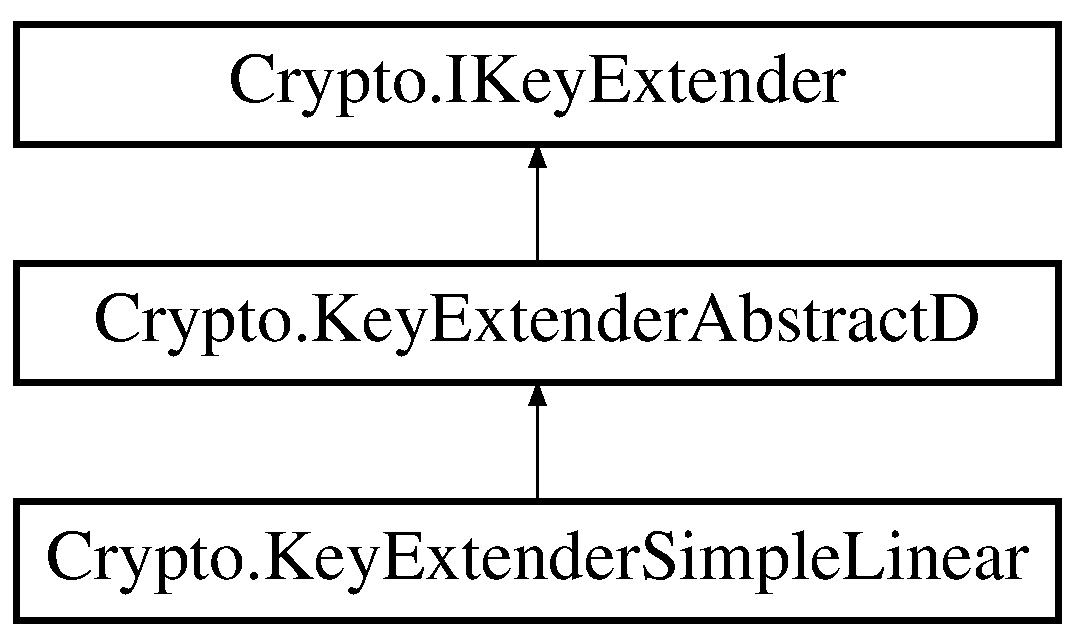
\includegraphics[height=3.000000cm]{class_crypto_1_1_key_extender_simple_linear}
\end{center}
\end{figure}
\subsection*{Public Member Functions}
\begin{DoxyCompactItemize}
\item 
\hyperlink{class_crypto_1_1_key_extender_simple_linear_a318ebefc5ef25570e751b21c071fba06}{Key\+Extender\+Simple\+Linear} (\hyperlink{interface_cellular_1_1_i_binary_c_a}{I\+Binary\+C\+A} binary\+C\+A)
\item 
override Bit\+Array \hyperlink{class_crypto_1_1_key_extender_simple_linear_a1b511ea8a0e0bb6cbd4f6a94f49015bd}{Double\+Key} (Bit\+Array short\+Key)
\begin{DoxyCompactList}\small\item\em Generates a longer key from a short key. \end{DoxyCompactList}\end{DoxyCompactItemize}


\subsection{Detailed Description}
Simple algorithm, which uses only two steps of the underlying C\+A. 



Definition at line 9 of file Key\+Extender\+Simple\+Linear.\+cs.



\subsection{Constructor \& Destructor Documentation}
\hypertarget{class_crypto_1_1_key_extender_simple_linear_a318ebefc5ef25570e751b21c071fba06}{}\index{Crypto\+::\+Key\+Extender\+Simple\+Linear@{Crypto\+::\+Key\+Extender\+Simple\+Linear}!Key\+Extender\+Simple\+Linear@{Key\+Extender\+Simple\+Linear}}
\index{Key\+Extender\+Simple\+Linear@{Key\+Extender\+Simple\+Linear}!Crypto\+::\+Key\+Extender\+Simple\+Linear@{Crypto\+::\+Key\+Extender\+Simple\+Linear}}
\subsubsection[{Key\+Extender\+Simple\+Linear(\+I\+Binary\+C\+A binary\+C\+A)}]{\setlength{\rightskip}{0pt plus 5cm}Crypto.\+Key\+Extender\+Simple\+Linear.\+Key\+Extender\+Simple\+Linear (
\begin{DoxyParamCaption}
\item[{{\bf I\+Binary\+C\+A}}]{binary\+C\+A}
\end{DoxyParamCaption}
)}\label{class_crypto_1_1_key_extender_simple_linear_a318ebefc5ef25570e751b21c071fba06}


Definition at line 13 of file Key\+Extender\+Simple\+Linear.\+cs.



\subsection{Member Function Documentation}
\hypertarget{class_crypto_1_1_key_extender_simple_linear_a1b511ea8a0e0bb6cbd4f6a94f49015bd}{}\index{Crypto\+::\+Key\+Extender\+Simple\+Linear@{Crypto\+::\+Key\+Extender\+Simple\+Linear}!Double\+Key@{Double\+Key}}
\index{Double\+Key@{Double\+Key}!Crypto\+::\+Key\+Extender\+Simple\+Linear@{Crypto\+::\+Key\+Extender\+Simple\+Linear}}
\subsubsection[{Double\+Key(\+Bit\+Array short\+Key)}]{\setlength{\rightskip}{0pt plus 5cm}override Bit\+Array Crypto.\+Key\+Extender\+Simple\+Linear.\+Double\+Key (
\begin{DoxyParamCaption}
\item[{Bit\+Array}]{short\+Key}
\end{DoxyParamCaption}
)\hspace{0.3cm}{\ttfamily [virtual]}}\label{class_crypto_1_1_key_extender_simple_linear_a1b511ea8a0e0bb6cbd4f6a94f49015bd}


Generates a longer key from a short key. 


\begin{DoxyParams}{Parameters}
{\em short\+Key} & Short key to be stretched (doubled).\\
\hline
\end{DoxyParams}
\begin{DoxyReturn}{Returns}
Long key (twice longer than input).
\end{DoxyReturn}


Implements \hyperlink{class_crypto_1_1_key_extender_abstract_d_ae403b92e9038b9c0bc7a21885e24ffc7}{Crypto.\+Key\+Extender\+Abstract\+D}.



Definition at line 18 of file Key\+Extender\+Simple\+Linear.\+cs.



The documentation for this class was generated from the following file\+:\begin{DoxyCompactItemize}
\item 
C\+:/\+Martin/\+M\+F\+F/\+\_\+baka/\+Martin\+Dvorak/\+Crypto/\hyperlink{_key_extender_simple_linear_8cs}{Key\+Extender\+Simple\+Linear.\+cs}\end{DoxyCompactItemize}

\hypertarget{class_crypto_1_1_key_extender_simple_quadratic}{}\section{Crypto.\+Key\+Extender\+Simple\+Quadratic Class Reference}
\label{class_crypto_1_1_key_extender_simple_quadratic}\index{Crypto.\+Key\+Extender\+Simple\+Quadratic@{Crypto.\+Key\+Extender\+Simple\+Quadratic}}


Simple algorithm, which calls one step of the underlying C\+A for every bit to be generated. Generating the long key may take a very long time.  


Inheritance diagram for Crypto.\+Key\+Extender\+Simple\+Quadratic\+:\begin{figure}[H]
\begin{center}
\leavevmode
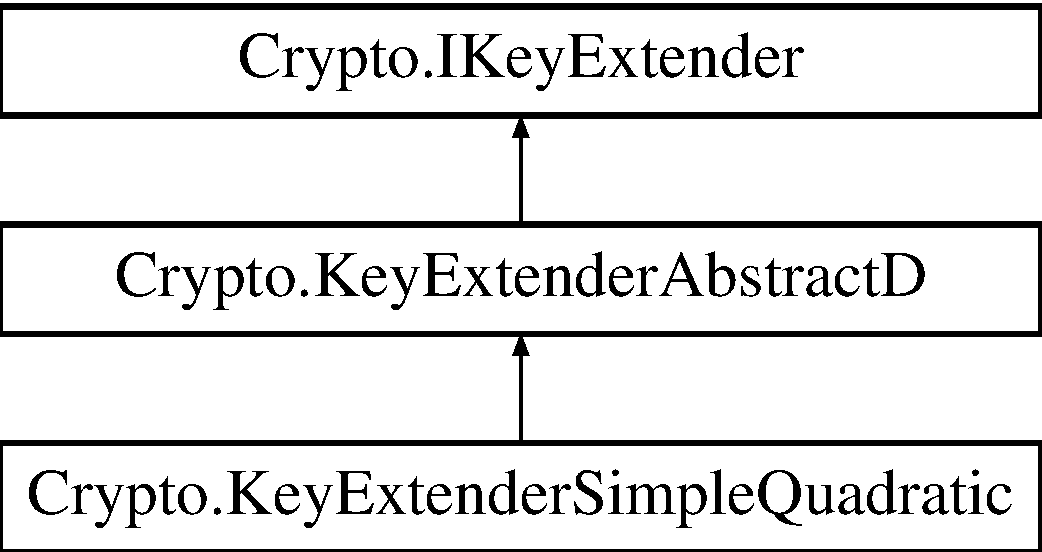
\includegraphics[height=3.000000cm]{class_crypto_1_1_key_extender_simple_quadratic}
\end{center}
\end{figure}
\subsection*{Public Member Functions}
\begin{DoxyCompactItemize}
\item 
\hyperlink{class_crypto_1_1_key_extender_simple_quadratic_a2090b48093409cd09a18c56ac7ec7826}{Key\+Extender\+Simple\+Quadratic} (\hyperlink{interface_cellular_1_1_i_binary_c_a}{I\+Binary\+C\+A} binary\+C\+A)
\item 
override Bit\+Array \hyperlink{class_crypto_1_1_key_extender_simple_quadratic_a0bba7646011678850879c0685d18b379}{Double\+Key} (Bit\+Array short\+Key)
\begin{DoxyCompactList}\small\item\em Generates a longer key from a short key. \end{DoxyCompactList}\end{DoxyCompactItemize}
\subsection*{Package Functions}
\begin{DoxyCompactItemize}
\item 
override string \hyperlink{class_crypto_1_1_key_extender_simple_quadratic_a4a399b40cd1893acf4cc8531771657a0}{Get\+Info} ()
\end{DoxyCompactItemize}


\subsection{Detailed Description}
Simple algorithm, which calls one step of the underlying C\+A for every bit to be generated. Generating the long key may take a very long time. 



Definition at line 10 of file Key\+Extender\+Simple\+Quadratic.\+cs.



\subsection{Constructor \& Destructor Documentation}
\hypertarget{class_crypto_1_1_key_extender_simple_quadratic_a2090b48093409cd09a18c56ac7ec7826}{}\index{Crypto\+::\+Key\+Extender\+Simple\+Quadratic@{Crypto\+::\+Key\+Extender\+Simple\+Quadratic}!Key\+Extender\+Simple\+Quadratic@{Key\+Extender\+Simple\+Quadratic}}
\index{Key\+Extender\+Simple\+Quadratic@{Key\+Extender\+Simple\+Quadratic}!Crypto\+::\+Key\+Extender\+Simple\+Quadratic@{Crypto\+::\+Key\+Extender\+Simple\+Quadratic}}
\subsubsection[{Key\+Extender\+Simple\+Quadratic(\+I\+Binary\+C\+A binary\+C\+A)}]{\setlength{\rightskip}{0pt plus 5cm}Crypto.\+Key\+Extender\+Simple\+Quadratic.\+Key\+Extender\+Simple\+Quadratic (
\begin{DoxyParamCaption}
\item[{{\bf I\+Binary\+C\+A}}]{binary\+C\+A}
\end{DoxyParamCaption}
)}\label{class_crypto_1_1_key_extender_simple_quadratic_a2090b48093409cd09a18c56ac7ec7826}


Definition at line 14 of file Key\+Extender\+Simple\+Quadratic.\+cs.



\subsection{Member Function Documentation}
\hypertarget{class_crypto_1_1_key_extender_simple_quadratic_a0bba7646011678850879c0685d18b379}{}\index{Crypto\+::\+Key\+Extender\+Simple\+Quadratic@{Crypto\+::\+Key\+Extender\+Simple\+Quadratic}!Double\+Key@{Double\+Key}}
\index{Double\+Key@{Double\+Key}!Crypto\+::\+Key\+Extender\+Simple\+Quadratic@{Crypto\+::\+Key\+Extender\+Simple\+Quadratic}}
\subsubsection[{Double\+Key(\+Bit\+Array short\+Key)}]{\setlength{\rightskip}{0pt plus 5cm}override Bit\+Array Crypto.\+Key\+Extender\+Simple\+Quadratic.\+Double\+Key (
\begin{DoxyParamCaption}
\item[{Bit\+Array}]{short\+Key}
\end{DoxyParamCaption}
)\hspace{0.3cm}{\ttfamily [virtual]}}\label{class_crypto_1_1_key_extender_simple_quadratic_a0bba7646011678850879c0685d18b379}


Generates a longer key from a short key. 


\begin{DoxyParams}{Parameters}
{\em short\+Key} & Short key to be stretched (doubled).\\
\hline
\end{DoxyParams}
\begin{DoxyReturn}{Returns}
Long key (twice longer than input).
\end{DoxyReturn}


Implements \hyperlink{class_crypto_1_1_key_extender_abstract_d_ae403b92e9038b9c0bc7a21885e24ffc7}{Crypto.\+Key\+Extender\+Abstract\+D}.



Definition at line 19 of file Key\+Extender\+Simple\+Quadratic.\+cs.

\hypertarget{class_crypto_1_1_key_extender_simple_quadratic_a4a399b40cd1893acf4cc8531771657a0}{}\index{Crypto\+::\+Key\+Extender\+Simple\+Quadratic@{Crypto\+::\+Key\+Extender\+Simple\+Quadratic}!Get\+Info@{Get\+Info}}
\index{Get\+Info@{Get\+Info}!Crypto\+::\+Key\+Extender\+Simple\+Quadratic@{Crypto\+::\+Key\+Extender\+Simple\+Quadratic}}
\subsubsection[{Get\+Info()}]{\setlength{\rightskip}{0pt plus 5cm}override string Crypto.\+Key\+Extender\+Simple\+Quadratic.\+Get\+Info (
\begin{DoxyParamCaption}
{}
\end{DoxyParamCaption}
)\hspace{0.3cm}{\ttfamily [package]}, {\ttfamily [virtual]}}\label{class_crypto_1_1_key_extender_simple_quadratic_a4a399b40cd1893acf4cc8531771657a0}


Implements \hyperlink{class_crypto_1_1_key_extender_abstract_d_a954261bd6f533ad7745beac9ce89dd6e}{Crypto.\+Key\+Extender\+Abstract\+D}.



Definition at line 40 of file Key\+Extender\+Simple\+Quadratic.\+cs.



The documentation for this class was generated from the following file\+:\begin{DoxyCompactItemize}
\item 
C\+:/\+Martin/\+M\+F\+F/\+\_\+baka/\+Martin\+Dvorak/\+Crypto/\hyperlink{_key_extender_simple_quadratic_8cs}{Key\+Extender\+Simple\+Quadratic.\+cs}\end{DoxyCompactItemize}

\hypertarget{class_crypto_1_1_key_extender_uncertain}{}\section{Crypto.\+Key\+Extender\+Uncertain Class Reference}
\label{class_crypto_1_1_key_extender_uncertain}\index{Crypto.\+Key\+Extender\+Uncertain@{Crypto.\+Key\+Extender\+Uncertain}}


Intelligent key extender that equalizes frequencies of 0 and 1, which may be different in the underlying C\+A. However it is not guaranteed that the long key will be generated.  


Inheritance diagram for Crypto.\+Key\+Extender\+Uncertain\+:\begin{figure}[H]
\begin{center}
\leavevmode
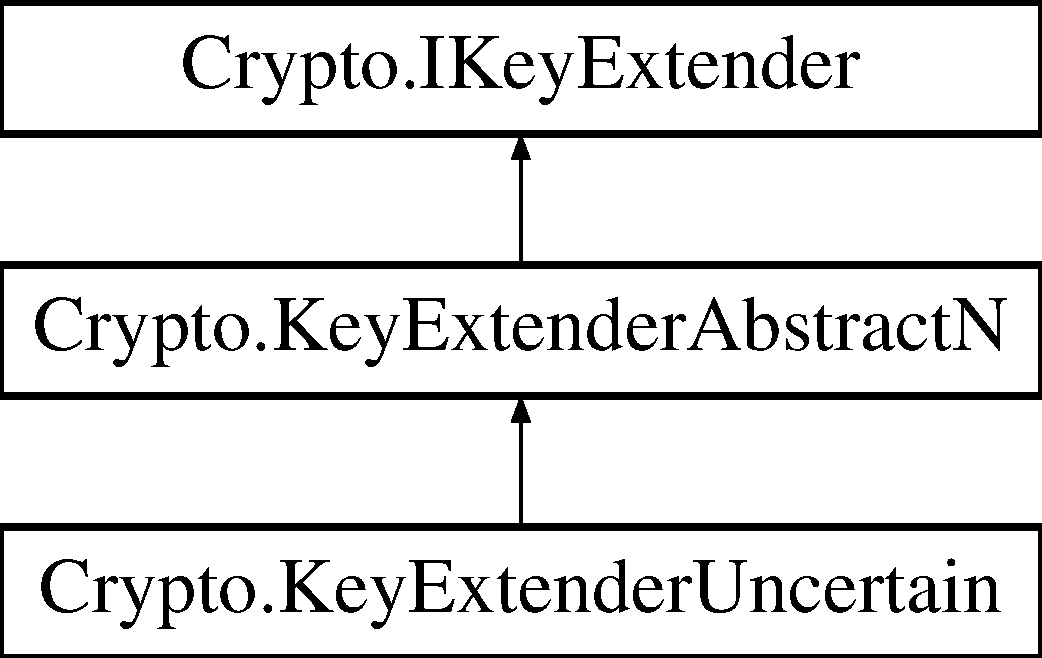
\includegraphics[height=3.000000cm]{class_crypto_1_1_key_extender_uncertain}
\end{center}
\end{figure}
\subsection*{Public Member Functions}
\begin{DoxyCompactItemize}
\item 
\hyperlink{class_crypto_1_1_key_extender_uncertain_aace64d24b92154a9e01002ee13e0b891}{Key\+Extender\+Uncertain} (\hyperlink{interface_cellular_1_1_i_binary_c_a}{I\+Binary\+C\+A} binary\+C\+A)
\item 
override Bit\+Array \hyperlink{class_crypto_1_1_key_extender_uncertain_a2955df98d2f4831576b12aa9c5ec609d}{Extend\+Key} (Bit\+Array short\+Key, int target\+Length)
\begin{DoxyCompactList}\small\item\em Generates a longer key from a short key. \end{DoxyCompactList}\end{DoxyCompactItemize}


\subsection{Detailed Description}
Intelligent key extender that equalizes frequencies of 0 and 1, which may be different in the underlying C\+A. However it is not guaranteed that the long key will be generated. 



Definition at line 12 of file Key\+Extender\+Uncertain.\+cs.



\subsection{Constructor \& Destructor Documentation}
\hypertarget{class_crypto_1_1_key_extender_uncertain_aace64d24b92154a9e01002ee13e0b891}{}\index{Crypto\+::\+Key\+Extender\+Uncertain@{Crypto\+::\+Key\+Extender\+Uncertain}!Key\+Extender\+Uncertain@{Key\+Extender\+Uncertain}}
\index{Key\+Extender\+Uncertain@{Key\+Extender\+Uncertain}!Crypto\+::\+Key\+Extender\+Uncertain@{Crypto\+::\+Key\+Extender\+Uncertain}}
\subsubsection[{Key\+Extender\+Uncertain(\+I\+Binary\+C\+A binary\+C\+A)}]{\setlength{\rightskip}{0pt plus 5cm}Crypto.\+Key\+Extender\+Uncertain.\+Key\+Extender\+Uncertain (
\begin{DoxyParamCaption}
\item[{{\bf I\+Binary\+C\+A}}]{binary\+C\+A}
\end{DoxyParamCaption}
)}\label{class_crypto_1_1_key_extender_uncertain_aace64d24b92154a9e01002ee13e0b891}


Definition at line 18 of file Key\+Extender\+Uncertain.\+cs.



\subsection{Member Function Documentation}
\hypertarget{class_crypto_1_1_key_extender_uncertain_a2955df98d2f4831576b12aa9c5ec609d}{}\index{Crypto\+::\+Key\+Extender\+Uncertain@{Crypto\+::\+Key\+Extender\+Uncertain}!Extend\+Key@{Extend\+Key}}
\index{Extend\+Key@{Extend\+Key}!Crypto\+::\+Key\+Extender\+Uncertain@{Crypto\+::\+Key\+Extender\+Uncertain}}
\subsubsection[{Extend\+Key(\+Bit\+Array short\+Key, int target\+Length)}]{\setlength{\rightskip}{0pt plus 5cm}override Bit\+Array Crypto.\+Key\+Extender\+Uncertain.\+Extend\+Key (
\begin{DoxyParamCaption}
\item[{Bit\+Array}]{short\+Key, }
\item[{int}]{target\+Length}
\end{DoxyParamCaption}
)\hspace{0.3cm}{\ttfamily [virtual]}}\label{class_crypto_1_1_key_extender_uncertain_a2955df98d2f4831576b12aa9c5ec609d}


Generates a longer key from a short key. 


\begin{DoxyParams}{Parameters}
{\em short\+Key} & Short key to be stretched (multiplied).\\
\hline
{\em target\+Length} & How many bits should the resulting long key have?\\
\hline
\end{DoxyParams}
\begin{DoxyReturn}{Returns}
Long key (of specified length).
\end{DoxyReturn}


Implements \hyperlink{class_crypto_1_1_key_extender_abstract_n_a9df4156ad0a84730f87119e5a25cf1ef}{Crypto.\+Key\+Extender\+Abstract\+N}.



Definition at line 23 of file Key\+Extender\+Uncertain.\+cs.



The documentation for this class was generated from the following file\+:\begin{DoxyCompactItemize}
\item 
C\+:/\+Martin/\+M\+F\+F/\+\_\+baka/\+Martin\+Dvorak/\+Crypto/\hyperlink{_key_extender_uncertain_8cs}{Key\+Extender\+Uncertain.\+cs}\end{DoxyCompactItemize}

\hypertarget{class_testing_1_1_main_tests}{}\section{Testing.\+Main\+Tests Class Reference}
\label{class_testing_1_1_main_tests}\index{Testing.\+Main\+Tests@{Testing.\+Main\+Tests}}


The most important tests (rating of key extenders) for my thesis.  


\subsection*{Static Public Member Functions}
\begin{DoxyCompactItemize}
\item 
static void \hyperlink{class_testing_1_1_main_tests_a013daeb576cbc0d58dfc82d8f5003806}{Run\+Test} ()
\begin{DoxyCompactList}\small\item\em Runs the most important tests for my thesis. \end{DoxyCompactList}\end{DoxyCompactItemize}


\subsection{Detailed Description}
The most important tests (rating of key extenders) for my thesis. 



Definition at line 11 of file Main\+Tests.\+cs.



\subsection{Member Function Documentation}
\hypertarget{class_testing_1_1_main_tests_a013daeb576cbc0d58dfc82d8f5003806}{}\index{Testing\+::\+Main\+Tests@{Testing\+::\+Main\+Tests}!Run\+Test@{Run\+Test}}
\index{Run\+Test@{Run\+Test}!Testing\+::\+Main\+Tests@{Testing\+::\+Main\+Tests}}
\subsubsection[{Run\+Test()}]{\setlength{\rightskip}{0pt plus 5cm}static void Testing.\+Main\+Tests.\+Run\+Test (
\begin{DoxyParamCaption}
{}
\end{DoxyParamCaption}
)\hspace{0.3cm}{\ttfamily [static]}}\label{class_testing_1_1_main_tests_a013daeb576cbc0d58dfc82d8f5003806}


Runs the most important tests for my thesis. 



Definition at line 16 of file Main\+Tests.\+cs.



The documentation for this class was generated from the following file\+:\begin{DoxyCompactItemize}
\item 
C\+:/\+Martin/\+M\+F\+F/\+\_\+baka/\+Martin\+Dvorak/\+Testing/\hyperlink{_main_tests_8cs}{Main\+Tests.\+cs}\end{DoxyCompactItemize}

\hypertarget{class_cellular_1_1_nary1_d_automaton}{}\section{Cellular.\+Nary1\+D\+Automaton Class Reference}
\label{class_cellular_1_1_nary1_d_automaton}\index{Cellular.\+Nary1\+D\+Automaton@{Cellular.\+Nary1\+D\+Automaton}}


Abstract class for general 1\+D N-\/ary automata.  


Inheritance diagram for Cellular.\+Nary1\+D\+Automaton\+:\begin{figure}[H]
\begin{center}
\leavevmode
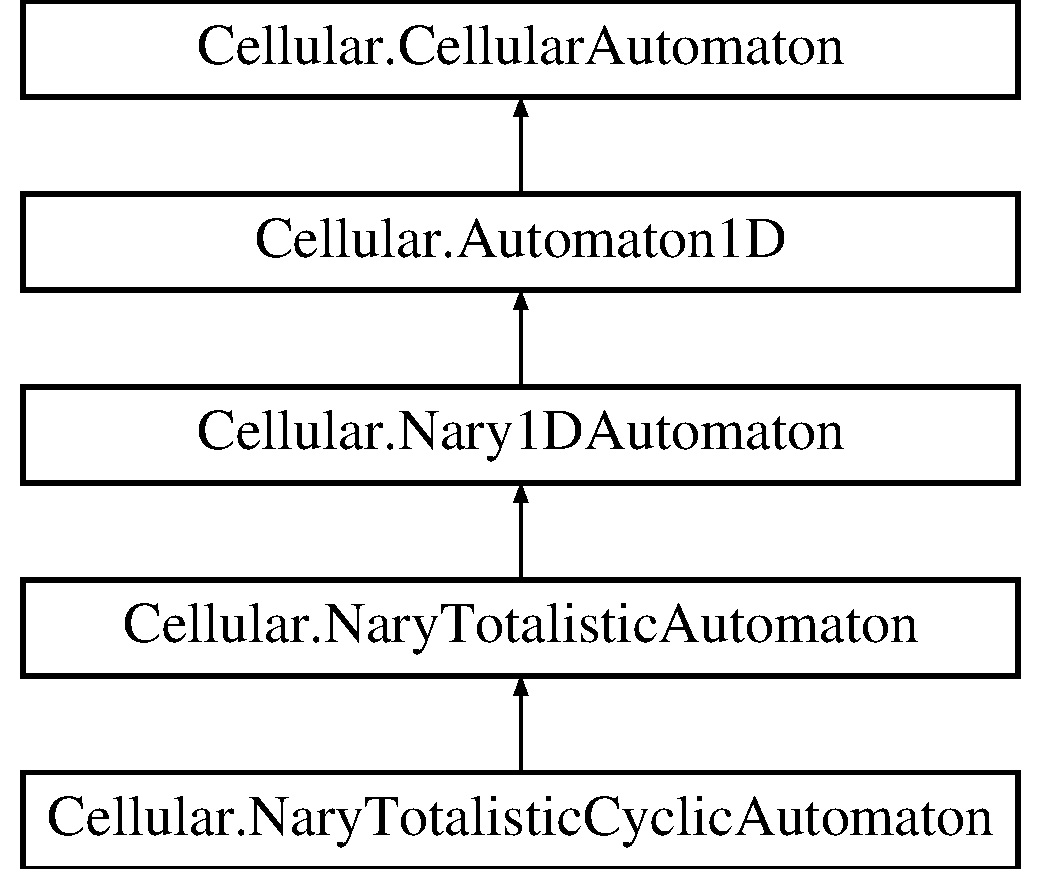
\includegraphics[height=5.000000cm]{class_cellular_1_1_nary1_d_automaton}
\end{center}
\end{figure}
\subsection*{Public Member Functions}
\begin{DoxyCompactItemize}
\item 
\hyperlink{class_cellular_1_1_nary1_d_automaton_a9b38ab16780bc9fb347f714bdd8f1295}{Nary1\+D\+Automaton} (int number\+Of\+States, int\mbox{[}$\,$\mbox{]} \hyperlink{all__1_8js_ae8b87ff4be2ae1dd5267342795263360}{initial\+State})
\item 
\hyperlink{class_cellular_1_1_nary1_d_automaton_ad9678852ba9ef44a300f2d272757d482}{Nary1\+D\+Automaton} (int number\+Of\+States, int \hyperlink{class_cellular_1_1_automaton1_d_a915129ccf0f1e7092844c99ce6a28e5b}{size}, Random rnd)
\end{DoxyCompactItemize}
\subsection*{Protected Member Functions}
\begin{DoxyCompactItemize}
\item 
virtual int \hyperlink{class_cellular_1_1_nary1_d_automaton_adfd39915b66667efeeb9b16f154b9b6b}{get\+Value\+At} (int index)
\begin{DoxyCompactList}\small\item\em This method simplifies boundary conditions. \end{DoxyCompactList}\end{DoxyCompactItemize}
\subsection*{Protected Attributes}
\begin{DoxyCompactItemize}
\item 
int \hyperlink{class_cellular_1_1_nary1_d_automaton_a1e499082e289666a6eb3d523d367ac1f}{N}
\item 
int\mbox{[}$\,$\mbox{]} \hyperlink{class_cellular_1_1_nary1_d_automaton_a563eb68c941321814d9261d68eed63f3}{state}
\end{DoxyCompactItemize}


\subsection{Detailed Description}
Abstract class for general 1\+D N-\/ary automata. 



Definition at line 8 of file Nary1\+D\+Automaton.\+cs.



\subsection{Constructor \& Destructor Documentation}
\hypertarget{class_cellular_1_1_nary1_d_automaton_a9b38ab16780bc9fb347f714bdd8f1295}{}\index{Cellular\+::\+Nary1\+D\+Automaton@{Cellular\+::\+Nary1\+D\+Automaton}!Nary1\+D\+Automaton@{Nary1\+D\+Automaton}}
\index{Nary1\+D\+Automaton@{Nary1\+D\+Automaton}!Cellular\+::\+Nary1\+D\+Automaton@{Cellular\+::\+Nary1\+D\+Automaton}}
\subsubsection[{Nary1\+D\+Automaton(int number\+Of\+States, int[] initial\+State)}]{\setlength{\rightskip}{0pt plus 5cm}Cellular.\+Nary1\+D\+Automaton.\+Nary1\+D\+Automaton (
\begin{DoxyParamCaption}
\item[{int}]{number\+Of\+States, }
\item[{int\mbox{[}$\,$\mbox{]}}]{initial\+State}
\end{DoxyParamCaption}
)}\label{class_cellular_1_1_nary1_d_automaton_a9b38ab16780bc9fb347f714bdd8f1295}


Definition at line 13 of file Nary1\+D\+Automaton.\+cs.

\hypertarget{class_cellular_1_1_nary1_d_automaton_ad9678852ba9ef44a300f2d272757d482}{}\index{Cellular\+::\+Nary1\+D\+Automaton@{Cellular\+::\+Nary1\+D\+Automaton}!Nary1\+D\+Automaton@{Nary1\+D\+Automaton}}
\index{Nary1\+D\+Automaton@{Nary1\+D\+Automaton}!Cellular\+::\+Nary1\+D\+Automaton@{Cellular\+::\+Nary1\+D\+Automaton}}
\subsubsection[{Nary1\+D\+Automaton(int number\+Of\+States, int size, Random rnd)}]{\setlength{\rightskip}{0pt plus 5cm}Cellular.\+Nary1\+D\+Automaton.\+Nary1\+D\+Automaton (
\begin{DoxyParamCaption}
\item[{int}]{number\+Of\+States, }
\item[{int}]{size, }
\item[{Random}]{rnd}
\end{DoxyParamCaption}
)}\label{class_cellular_1_1_nary1_d_automaton_ad9678852ba9ef44a300f2d272757d482}


Definition at line 20 of file Nary1\+D\+Automaton.\+cs.



\subsection{Member Function Documentation}
\hypertarget{class_cellular_1_1_nary1_d_automaton_adfd39915b66667efeeb9b16f154b9b6b}{}\index{Cellular\+::\+Nary1\+D\+Automaton@{Cellular\+::\+Nary1\+D\+Automaton}!get\+Value\+At@{get\+Value\+At}}
\index{get\+Value\+At@{get\+Value\+At}!Cellular\+::\+Nary1\+D\+Automaton@{Cellular\+::\+Nary1\+D\+Automaton}}
\subsubsection[{get\+Value\+At(int index)}]{\setlength{\rightskip}{0pt plus 5cm}virtual int Cellular.\+Nary1\+D\+Automaton.\+get\+Value\+At (
\begin{DoxyParamCaption}
\item[{int}]{index}
\end{DoxyParamCaption}
)\hspace{0.3cm}{\ttfamily [protected]}, {\ttfamily [virtual]}}\label{class_cellular_1_1_nary1_d_automaton_adfd39915b66667efeeb9b16f154b9b6b}


This method simplifies boundary conditions. 


\begin{DoxyParams}{Parameters}
{\em index} & Zero-\/based index (which value is required).\\
\hline
\end{DoxyParams}
\begin{DoxyReturn}{Returns}
Value from 0 to N-\/1.
\end{DoxyReturn}


Reimplemented in \hyperlink{class_cellular_1_1_nary_totalistic_cyclic_automaton_a422dbcbd3e3cd3efdccc21724e7c6b01}{Cellular.\+Nary\+Totalistic\+Cyclic\+Automaton}.



Definition at line 35 of file Nary1\+D\+Automaton.\+cs.



\subsection{Member Data Documentation}
\hypertarget{class_cellular_1_1_nary1_d_automaton_a1e499082e289666a6eb3d523d367ac1f}{}\index{Cellular\+::\+Nary1\+D\+Automaton@{Cellular\+::\+Nary1\+D\+Automaton}!N@{N}}
\index{N@{N}!Cellular\+::\+Nary1\+D\+Automaton@{Cellular\+::\+Nary1\+D\+Automaton}}
\subsubsection[{N}]{\setlength{\rightskip}{0pt plus 5cm}int Cellular.\+Nary1\+D\+Automaton.\+N\hspace{0.3cm}{\ttfamily [protected]}}\label{class_cellular_1_1_nary1_d_automaton_a1e499082e289666a6eb3d523d367ac1f}


Definition at line 10 of file Nary1\+D\+Automaton.\+cs.

\hypertarget{class_cellular_1_1_nary1_d_automaton_a563eb68c941321814d9261d68eed63f3}{}\index{Cellular\+::\+Nary1\+D\+Automaton@{Cellular\+::\+Nary1\+D\+Automaton}!state@{state}}
\index{state@{state}!Cellular\+::\+Nary1\+D\+Automaton@{Cellular\+::\+Nary1\+D\+Automaton}}
\subsubsection[{state}]{\setlength{\rightskip}{0pt plus 5cm}int \mbox{[}$\,$\mbox{]} Cellular.\+Nary1\+D\+Automaton.\+state\hspace{0.3cm}{\ttfamily [protected]}}\label{class_cellular_1_1_nary1_d_automaton_a563eb68c941321814d9261d68eed63f3}


Definition at line 11 of file Nary1\+D\+Automaton.\+cs.



The documentation for this class was generated from the following file\+:\begin{DoxyCompactItemize}
\item 
C\+:/\+Martin/\+M\+F\+F/\+\_\+baka/\+Martin\+Dvorak/\+Cellular/\hyperlink{_nary1_d_automaton_8cs}{Nary1\+D\+Automaton.\+cs}\end{DoxyCompactItemize}

\hypertarget{class_cellular_1_1_nary_totalistic_automaton}{}\section{Cellular.\+Nary\+Totalistic\+Automaton Class Reference}
\label{class_cellular_1_1_nary_totalistic_automaton}\index{Cellular.\+Nary\+Totalistic\+Automaton@{Cellular.\+Nary\+Totalistic\+Automaton}}


Class representing any n-\/ary one-\/dimensional automaton with a totalistic rule -\/ bordered variant. The new state of each cell depends on the sum of its current state and the current state of adjecent cells.  


Inheritance diagram for Cellular.\+Nary\+Totalistic\+Automaton\+:\begin{figure}[H]
\begin{center}
\leavevmode
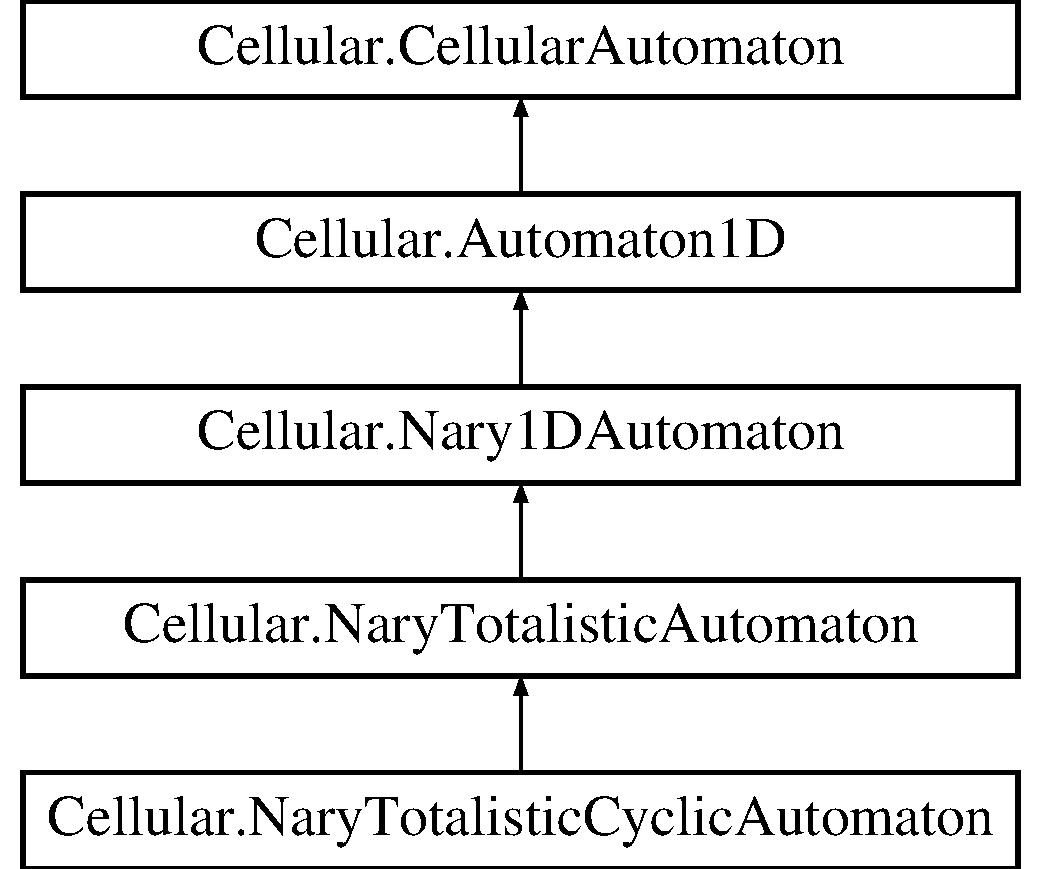
\includegraphics[height=5.000000cm]{class_cellular_1_1_nary_totalistic_automaton}
\end{center}
\end{figure}
\subsection*{Public Member Functions}
\begin{DoxyCompactItemize}
\item 
\hyperlink{class_cellular_1_1_nary_totalistic_automaton_aafe92ae99ccbb3591b128d6e720227f6}{Nary\+Totalistic\+Automaton} (int number\+Of\+States, int\mbox{[}$\,$\mbox{]} \hyperlink{class_cellular_1_1_nary_totalistic_automaton_a878c767c6823bd8ed8dc0f7d2ccb1fd2}{rule}, int\mbox{[}$\,$\mbox{]} \hyperlink{all__1_8js_ae8b87ff4be2ae1dd5267342795263360}{initial\+State})
\begin{DoxyCompactList}\small\item\em Creates a new totalistic N-\/ary automaton with given rule and initial state. \end{DoxyCompactList}\item 
override void \hyperlink{class_cellular_1_1_nary_totalistic_automaton_ad90769a438ab94b46d4750a571782056}{Step} ()
\begin{DoxyCompactList}\small\item\em Performs one step applying the specific rule for creating a new state. \end{DoxyCompactList}\item 
override object \hyperlink{class_cellular_1_1_nary_totalistic_automaton_a13f16113915ecec451fc4764a32044f9}{Clone} ()
\begin{DoxyCompactList}\small\item\em Creates an appropriate copy of the C\+A. Its type and the specific rule are always preserved. However, the time (number of steps executed on the specific instance) is set back to 0. \end{DoxyCompactList}\item 
override string \hyperlink{class_cellular_1_1_nary_totalistic_automaton_aa691c532a55638c7e3d0c125a4244773}{Tell\+Type} ()
\begin{DoxyCompactList}\small\item\em Announces the runtime type of the C\+A including info about its rule. It serves for debugging purposes. \end{DoxyCompactList}\item 
string \hyperlink{class_cellular_1_1_nary_totalistic_automaton_a239c8e21ae35741c4baadb96be21cec9}{Print\+Ternary} ()
\begin{DoxyCompactList}\small\item\em Converts the inner state into a well-\/printable string. This method works best for ternary (N=3) automata. \end{DoxyCompactList}\item 
string \hyperlink{class_cellular_1_1_nary_totalistic_automaton_aa9d5e154d625d8a8884221df45766145}{Print\+Quinary} ()
\begin{DoxyCompactList}\small\item\em Converts the inner state into a well-\/printable string. This method works best for quinary (N=5) automata. \end{DoxyCompactList}\end{DoxyCompactItemize}
\subsection*{Protected Attributes}
\begin{DoxyCompactItemize}
\item 
int\mbox{[}$\,$\mbox{]} \hyperlink{class_cellular_1_1_nary_totalistic_automaton_a878c767c6823bd8ed8dc0f7d2ccb1fd2}{rule}
\end{DoxyCompactItemize}
\subsection*{Additional Inherited Members}


\subsection{Detailed Description}
Class representing any n-\/ary one-\/dimensional automaton with a totalistic rule -\/ bordered variant. The new state of each cell depends on the sum of its current state and the current state of adjecent cells. 



Definition at line 9 of file Nary\+Totalistic\+Automaton.\+cs.



\subsection{Constructor \& Destructor Documentation}
\hypertarget{class_cellular_1_1_nary_totalistic_automaton_aafe92ae99ccbb3591b128d6e720227f6}{}\index{Cellular\+::\+Nary\+Totalistic\+Automaton@{Cellular\+::\+Nary\+Totalistic\+Automaton}!Nary\+Totalistic\+Automaton@{Nary\+Totalistic\+Automaton}}
\index{Nary\+Totalistic\+Automaton@{Nary\+Totalistic\+Automaton}!Cellular\+::\+Nary\+Totalistic\+Automaton@{Cellular\+::\+Nary\+Totalistic\+Automaton}}
\subsubsection[{Nary\+Totalistic\+Automaton(int number\+Of\+States, int[] rule, int[] initial\+State)}]{\setlength{\rightskip}{0pt plus 5cm}Cellular.\+Nary\+Totalistic\+Automaton.\+Nary\+Totalistic\+Automaton (
\begin{DoxyParamCaption}
\item[{int}]{number\+Of\+States, }
\item[{int\mbox{[}$\,$\mbox{]}}]{rule, }
\item[{int\mbox{[}$\,$\mbox{]}}]{initial\+State}
\end{DoxyParamCaption}
)}\label{class_cellular_1_1_nary_totalistic_automaton_aafe92ae99ccbb3591b128d6e720227f6}


Creates a new totalistic N-\/ary automaton with given rule and initial state. 


\begin{DoxyParams}{Parameters}
{\em number\+Of\+States} & The N.\\
\hline
{\em rule} & Array representing the rule for creating a new state. Value in rule\mbox{[}0\mbox{]} determines what happens to a white (0/dead) cell with white immediate neighbours. Value in rule\mbox{[}3$\ast$(N-\/1)\mbox{]} determines what happens to a black (max\+Val) cell with black immediate neighbours.\\
\hline
{\em initial\+State} & An integer array describing the initial state of the C\+A. This also determines the size of the new C\+A.\\
\hline
\end{DoxyParams}


Definition at line 22 of file Nary\+Totalistic\+Automaton.\+cs.



\subsection{Member Function Documentation}
\hypertarget{class_cellular_1_1_nary_totalistic_automaton_a13f16113915ecec451fc4764a32044f9}{}\index{Cellular\+::\+Nary\+Totalistic\+Automaton@{Cellular\+::\+Nary\+Totalistic\+Automaton}!Clone@{Clone}}
\index{Clone@{Clone}!Cellular\+::\+Nary\+Totalistic\+Automaton@{Cellular\+::\+Nary\+Totalistic\+Automaton}}
\subsubsection[{Clone()}]{\setlength{\rightskip}{0pt plus 5cm}override object Cellular.\+Nary\+Totalistic\+Automaton.\+Clone (
\begin{DoxyParamCaption}
{}
\end{DoxyParamCaption}
)\hspace{0.3cm}{\ttfamily [virtual]}}\label{class_cellular_1_1_nary_totalistic_automaton_a13f16113915ecec451fc4764a32044f9}


Creates an appropriate copy of the C\+A. Its type and the specific rule are always preserved. However, the time (number of steps executed on the specific instance) is set back to 0. 

\begin{DoxyReturn}{Returns}
A copy of the {\ttfamily \hyperlink{class_cellular_1_1_cellular_automaton}{Cellular\+Automaton}} as an {\ttfamily Object}
\end{DoxyReturn}


Implements \hyperlink{class_cellular_1_1_cellular_automaton_affd487b397cdbbbb1982815bbcd8e7d3}{Cellular.\+Cellular\+Automaton}.



Reimplemented in \hyperlink{class_cellular_1_1_nary_totalistic_cyclic_automaton_aa8d5a7d77a6dfc5f6e4fae6ba1c6cfd0}{Cellular.\+Nary\+Totalistic\+Cyclic\+Automaton}.



Definition at line 37 of file Nary\+Totalistic\+Automaton.\+cs.

\hypertarget{class_cellular_1_1_nary_totalistic_automaton_aa9d5e154d625d8a8884221df45766145}{}\index{Cellular\+::\+Nary\+Totalistic\+Automaton@{Cellular\+::\+Nary\+Totalistic\+Automaton}!Print\+Quinary@{Print\+Quinary}}
\index{Print\+Quinary@{Print\+Quinary}!Cellular\+::\+Nary\+Totalistic\+Automaton@{Cellular\+::\+Nary\+Totalistic\+Automaton}}
\subsubsection[{Print\+Quinary()}]{\setlength{\rightskip}{0pt plus 5cm}string Cellular.\+Nary\+Totalistic\+Automaton.\+Print\+Quinary (
\begin{DoxyParamCaption}
{}
\end{DoxyParamCaption}
)}\label{class_cellular_1_1_nary_totalistic_automaton_aa9d5e154d625d8a8884221df45766145}


Converts the inner state into a well-\/printable string. This method works best for quinary (N=5) automata. 

\begin{DoxyReturn}{Returns}
String consisting of different shades of rectangles. All values 4+ are represented by a full rectangle.
\end{DoxyReturn}


Definition at line 70 of file Nary\+Totalistic\+Automaton.\+cs.

\hypertarget{class_cellular_1_1_nary_totalistic_automaton_a239c8e21ae35741c4baadb96be21cec9}{}\index{Cellular\+::\+Nary\+Totalistic\+Automaton@{Cellular\+::\+Nary\+Totalistic\+Automaton}!Print\+Ternary@{Print\+Ternary}}
\index{Print\+Ternary@{Print\+Ternary}!Cellular\+::\+Nary\+Totalistic\+Automaton@{Cellular\+::\+Nary\+Totalistic\+Automaton}}
\subsubsection[{Print\+Ternary()}]{\setlength{\rightskip}{0pt plus 5cm}string Cellular.\+Nary\+Totalistic\+Automaton.\+Print\+Ternary (
\begin{DoxyParamCaption}
{}
\end{DoxyParamCaption}
)}\label{class_cellular_1_1_nary_totalistic_automaton_a239c8e21ae35741c4baadb96be21cec9}


Converts the inner state into a well-\/printable string. This method works best for ternary (N=3) automata. 

\begin{DoxyReturn}{Returns}
String consisting of different shades of rectangles. All values 2+ are represented by a full rectangle.
\end{DoxyReturn}


Definition at line 51 of file Nary\+Totalistic\+Automaton.\+cs.

\hypertarget{class_cellular_1_1_nary_totalistic_automaton_ad90769a438ab94b46d4750a571782056}{}\index{Cellular\+::\+Nary\+Totalistic\+Automaton@{Cellular\+::\+Nary\+Totalistic\+Automaton}!Step@{Step}}
\index{Step@{Step}!Cellular\+::\+Nary\+Totalistic\+Automaton@{Cellular\+::\+Nary\+Totalistic\+Automaton}}
\subsubsection[{Step()}]{\setlength{\rightskip}{0pt plus 5cm}override void Cellular.\+Nary\+Totalistic\+Automaton.\+Step (
\begin{DoxyParamCaption}
{}
\end{DoxyParamCaption}
)\hspace{0.3cm}{\ttfamily [virtual]}}\label{class_cellular_1_1_nary_totalistic_automaton_ad90769a438ab94b46d4750a571782056}


Performs one step applying the specific rule for creating a new state. 



Implements \hyperlink{class_cellular_1_1_cellular_automaton_aa70848d58015575974bc875ac5a89ae7}{Cellular.\+Cellular\+Automaton}.



Definition at line 27 of file Nary\+Totalistic\+Automaton.\+cs.

\hypertarget{class_cellular_1_1_nary_totalistic_automaton_aa691c532a55638c7e3d0c125a4244773}{}\index{Cellular\+::\+Nary\+Totalistic\+Automaton@{Cellular\+::\+Nary\+Totalistic\+Automaton}!Tell\+Type@{Tell\+Type}}
\index{Tell\+Type@{Tell\+Type}!Cellular\+::\+Nary\+Totalistic\+Automaton@{Cellular\+::\+Nary\+Totalistic\+Automaton}}
\subsubsection[{Tell\+Type()}]{\setlength{\rightskip}{0pt plus 5cm}override string Cellular.\+Nary\+Totalistic\+Automaton.\+Tell\+Type (
\begin{DoxyParamCaption}
{}
\end{DoxyParamCaption}
)\hspace{0.3cm}{\ttfamily [virtual]}}\label{class_cellular_1_1_nary_totalistic_automaton_aa691c532a55638c7e3d0c125a4244773}


Announces the runtime type of the C\+A including info about its rule. It serves for debugging purposes. 

\begin{DoxyReturn}{Returns}
Type of the C\+A as a string.
\end{DoxyReturn}


Implements \hyperlink{class_cellular_1_1_cellular_automaton_abe4b92fd405530c8a08cc07a3a19fff4}{Cellular.\+Cellular\+Automaton}.



Reimplemented in \hyperlink{class_cellular_1_1_nary_totalistic_cyclic_automaton_ac5c39cfb72386e3ab6132ab420091ae9}{Cellular.\+Nary\+Totalistic\+Cyclic\+Automaton}.



Definition at line 42 of file Nary\+Totalistic\+Automaton.\+cs.



\subsection{Member Data Documentation}
\hypertarget{class_cellular_1_1_nary_totalistic_automaton_a878c767c6823bd8ed8dc0f7d2ccb1fd2}{}\index{Cellular\+::\+Nary\+Totalistic\+Automaton@{Cellular\+::\+Nary\+Totalistic\+Automaton}!rule@{rule}}
\index{rule@{rule}!Cellular\+::\+Nary\+Totalistic\+Automaton@{Cellular\+::\+Nary\+Totalistic\+Automaton}}
\subsubsection[{rule}]{\setlength{\rightskip}{0pt plus 5cm}int \mbox{[}$\,$\mbox{]} Cellular.\+Nary\+Totalistic\+Automaton.\+rule\hspace{0.3cm}{\ttfamily [protected]}}\label{class_cellular_1_1_nary_totalistic_automaton_a878c767c6823bd8ed8dc0f7d2ccb1fd2}


Definition at line 11 of file Nary\+Totalistic\+Automaton.\+cs.



The documentation for this class was generated from the following file\+:\begin{DoxyCompactItemize}
\item 
C\+:/\+Martin/\+M\+F\+F/\+\_\+baka/\+Martin\+Dvorak/\+Cellular/\hyperlink{_nary_totalistic_automaton_8cs}{Nary\+Totalistic\+Automaton.\+cs}\end{DoxyCompactItemize}

\hypertarget{class_cellular_1_1_nary_totalistic_cyclic_automaton}{}\section{Cellular.\+Nary\+Totalistic\+Cyclic\+Automaton Class Reference}
\label{class_cellular_1_1_nary_totalistic_cyclic_automaton}\index{Cellular.\+Nary\+Totalistic\+Cyclic\+Automaton@{Cellular.\+Nary\+Totalistic\+Cyclic\+Automaton}}


Class representing any N-\/ary one-\/dimensional automaton with a totalistic rule -\/ cyclic variant. The new state of each cell depends on the sum of its current state and the current state of adjecent cells.  


Inheritance diagram for Cellular.\+Nary\+Totalistic\+Cyclic\+Automaton\+:\begin{figure}[H]
\begin{center}
\leavevmode
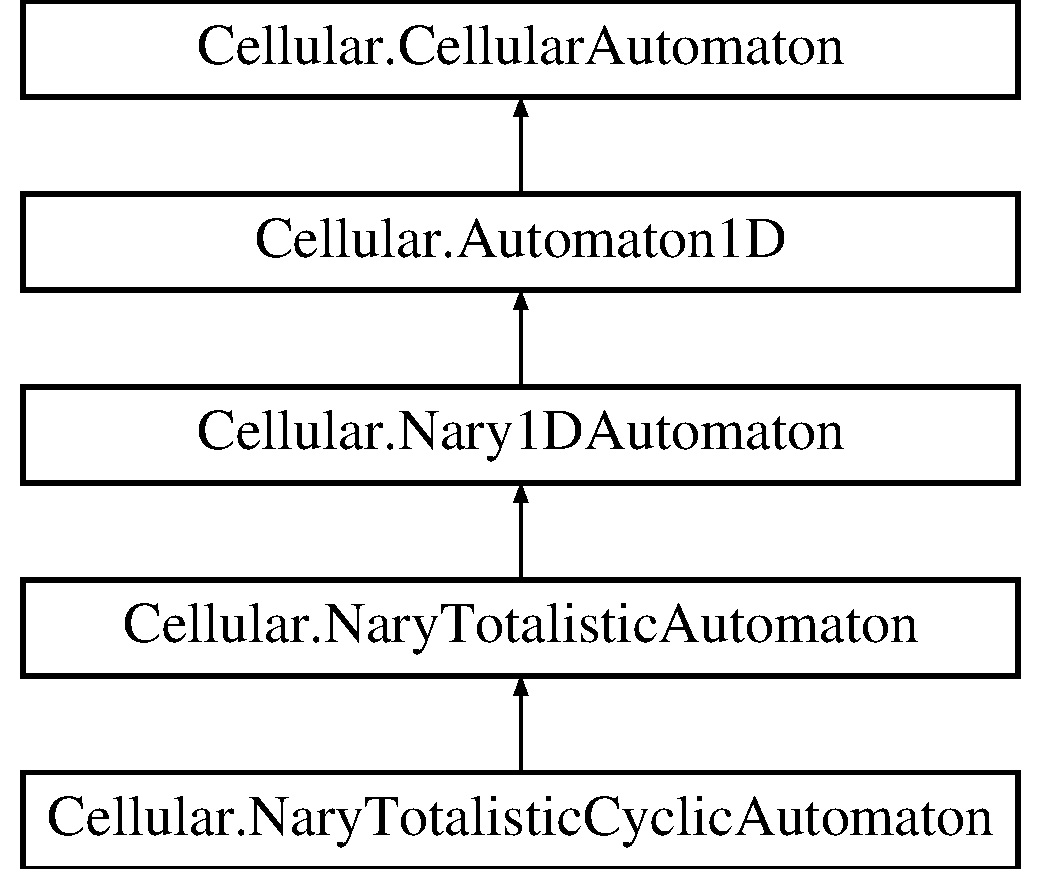
\includegraphics[height=5.000000cm]{class_cellular_1_1_nary_totalistic_cyclic_automaton}
\end{center}
\end{figure}
\subsection*{Public Member Functions}
\begin{DoxyCompactItemize}
\item 
\hyperlink{class_cellular_1_1_nary_totalistic_cyclic_automaton_a4616b10ffadcaef7a2d21b47976844af}{Nary\+Totalistic\+Cyclic\+Automaton} (int number\+Of\+States, int\mbox{[}$\,$\mbox{]} \hyperlink{class_cellular_1_1_nary_totalistic_automaton_a878c767c6823bd8ed8dc0f7d2ccb1fd2}{rule}, int\mbox{[}$\,$\mbox{]} initial\+State)
\item 
override object \hyperlink{class_cellular_1_1_nary_totalistic_cyclic_automaton_aa8d5a7d77a6dfc5f6e4fae6ba1c6cfd0}{Clone} ()
\begin{DoxyCompactList}\small\item\em Creates an appropriate copy of the C\+A. Its type and the specific rule are always preserved. However, the time (number of steps executed on the specific instance) is set back to 0. \end{DoxyCompactList}\item 
override string \hyperlink{class_cellular_1_1_nary_totalistic_cyclic_automaton_ac5c39cfb72386e3ab6132ab420091ae9}{Tell\+Type} ()
\begin{DoxyCompactList}\small\item\em Announces the runtime type of the C\+A including info about its rule. It serves for debugging purposes. \end{DoxyCompactList}\end{DoxyCompactItemize}
\subsection*{Protected Member Functions}
\begin{DoxyCompactItemize}
\item 
override int \hyperlink{class_cellular_1_1_nary_totalistic_cyclic_automaton_a422dbcbd3e3cd3efdccc21724e7c6b01}{get\+Value\+At} (int index)
\begin{DoxyCompactList}\small\item\em This method simplifies boundary conditions. \end{DoxyCompactList}\end{DoxyCompactItemize}
\subsection*{Additional Inherited Members}


\subsection{Detailed Description}
Class representing any N-\/ary one-\/dimensional automaton with a totalistic rule -\/ cyclic variant. The new state of each cell depends on the sum of its current state and the current state of adjecent cells. 



Definition at line 7 of file Nary\+Totalistic\+Cyclic\+Automaton.\+cs.



\subsection{Constructor \& Destructor Documentation}
\hypertarget{class_cellular_1_1_nary_totalistic_cyclic_automaton_a4616b10ffadcaef7a2d21b47976844af}{}\index{Cellular\+::\+Nary\+Totalistic\+Cyclic\+Automaton@{Cellular\+::\+Nary\+Totalistic\+Cyclic\+Automaton}!Nary\+Totalistic\+Cyclic\+Automaton@{Nary\+Totalistic\+Cyclic\+Automaton}}
\index{Nary\+Totalistic\+Cyclic\+Automaton@{Nary\+Totalistic\+Cyclic\+Automaton}!Cellular\+::\+Nary\+Totalistic\+Cyclic\+Automaton@{Cellular\+::\+Nary\+Totalistic\+Cyclic\+Automaton}}
\subsubsection[{Nary\+Totalistic\+Cyclic\+Automaton(int number\+Of\+States, int[] rule, int[] initial\+State)}]{\setlength{\rightskip}{0pt plus 5cm}Cellular.\+Nary\+Totalistic\+Cyclic\+Automaton.\+Nary\+Totalistic\+Cyclic\+Automaton (
\begin{DoxyParamCaption}
\item[{int}]{number\+Of\+States, }
\item[{int\mbox{[}$\,$\mbox{]}}]{rule, }
\item[{int\mbox{[}$\,$\mbox{]}}]{initial\+State}
\end{DoxyParamCaption}
)}\label{class_cellular_1_1_nary_totalistic_cyclic_automaton_a4616b10ffadcaef7a2d21b47976844af}


Definition at line 9 of file Nary\+Totalistic\+Cyclic\+Automaton.\+cs.



\subsection{Member Function Documentation}
\hypertarget{class_cellular_1_1_nary_totalistic_cyclic_automaton_aa8d5a7d77a6dfc5f6e4fae6ba1c6cfd0}{}\index{Cellular\+::\+Nary\+Totalistic\+Cyclic\+Automaton@{Cellular\+::\+Nary\+Totalistic\+Cyclic\+Automaton}!Clone@{Clone}}
\index{Clone@{Clone}!Cellular\+::\+Nary\+Totalistic\+Cyclic\+Automaton@{Cellular\+::\+Nary\+Totalistic\+Cyclic\+Automaton}}
\subsubsection[{Clone()}]{\setlength{\rightskip}{0pt plus 5cm}override object Cellular.\+Nary\+Totalistic\+Cyclic\+Automaton.\+Clone (
\begin{DoxyParamCaption}
{}
\end{DoxyParamCaption}
)\hspace{0.3cm}{\ttfamily [virtual]}}\label{class_cellular_1_1_nary_totalistic_cyclic_automaton_aa8d5a7d77a6dfc5f6e4fae6ba1c6cfd0}


Creates an appropriate copy of the C\+A. Its type and the specific rule are always preserved. However, the time (number of steps executed on the specific instance) is set back to 0. 

\begin{DoxyReturn}{Returns}
A copy of the {\ttfamily \hyperlink{class_cellular_1_1_cellular_automaton}{Cellular\+Automaton}} as an {\ttfamily Object}
\end{DoxyReturn}


Reimplemented from \hyperlink{class_cellular_1_1_nary_totalistic_automaton_a13f16113915ecec451fc4764a32044f9}{Cellular.\+Nary\+Totalistic\+Automaton}.



Definition at line 20 of file Nary\+Totalistic\+Cyclic\+Automaton.\+cs.

\hypertarget{class_cellular_1_1_nary_totalistic_cyclic_automaton_a422dbcbd3e3cd3efdccc21724e7c6b01}{}\index{Cellular\+::\+Nary\+Totalistic\+Cyclic\+Automaton@{Cellular\+::\+Nary\+Totalistic\+Cyclic\+Automaton}!get\+Value\+At@{get\+Value\+At}}
\index{get\+Value\+At@{get\+Value\+At}!Cellular\+::\+Nary\+Totalistic\+Cyclic\+Automaton@{Cellular\+::\+Nary\+Totalistic\+Cyclic\+Automaton}}
\subsubsection[{get\+Value\+At(int index)}]{\setlength{\rightskip}{0pt plus 5cm}override int Cellular.\+Nary\+Totalistic\+Cyclic\+Automaton.\+get\+Value\+At (
\begin{DoxyParamCaption}
\item[{int}]{index}
\end{DoxyParamCaption}
)\hspace{0.3cm}{\ttfamily [protected]}, {\ttfamily [virtual]}}\label{class_cellular_1_1_nary_totalistic_cyclic_automaton_a422dbcbd3e3cd3efdccc21724e7c6b01}


This method simplifies boundary conditions. 


\begin{DoxyParams}{Parameters}
{\em index} & Zero-\/based index (which value is required).\\
\hline
\end{DoxyParams}
\begin{DoxyReturn}{Returns}
Value from 0 to N-\/1.
\end{DoxyReturn}


Reimplemented from \hyperlink{class_cellular_1_1_nary1_d_automaton_adfd39915b66667efeeb9b16f154b9b6b}{Cellular.\+Nary1\+D\+Automaton}.



Definition at line 11 of file Nary\+Totalistic\+Cyclic\+Automaton.\+cs.

\hypertarget{class_cellular_1_1_nary_totalistic_cyclic_automaton_ac5c39cfb72386e3ab6132ab420091ae9}{}\index{Cellular\+::\+Nary\+Totalistic\+Cyclic\+Automaton@{Cellular\+::\+Nary\+Totalistic\+Cyclic\+Automaton}!Tell\+Type@{Tell\+Type}}
\index{Tell\+Type@{Tell\+Type}!Cellular\+::\+Nary\+Totalistic\+Cyclic\+Automaton@{Cellular\+::\+Nary\+Totalistic\+Cyclic\+Automaton}}
\subsubsection[{Tell\+Type()}]{\setlength{\rightskip}{0pt plus 5cm}override string Cellular.\+Nary\+Totalistic\+Cyclic\+Automaton.\+Tell\+Type (
\begin{DoxyParamCaption}
{}
\end{DoxyParamCaption}
)\hspace{0.3cm}{\ttfamily [virtual]}}\label{class_cellular_1_1_nary_totalistic_cyclic_automaton_ac5c39cfb72386e3ab6132ab420091ae9}


Announces the runtime type of the C\+A including info about its rule. It serves for debugging purposes. 

\begin{DoxyReturn}{Returns}
Type of the C\+A as a string.
\end{DoxyReturn}


Reimplemented from \hyperlink{class_cellular_1_1_nary_totalistic_automaton_aa691c532a55638c7e3d0c125a4244773}{Cellular.\+Nary\+Totalistic\+Automaton}.



Definition at line 25 of file Nary\+Totalistic\+Cyclic\+Automaton.\+cs.



The documentation for this class was generated from the following file\+:\begin{DoxyCompactItemize}
\item 
C\+:/\+Martin/\+M\+F\+F/\+\_\+baka/\+Martin\+Dvorak/\+Cellular/\hyperlink{_nary_totalistic_cyclic_automaton_8cs}{Nary\+Totalistic\+Cyclic\+Automaton.\+cs}\end{DoxyCompactItemize}

\hypertarget{class_program_1_1_program}{}\section{Program.\+Program Class Reference}
\label{class_program_1_1_program}\index{Program.\+Program@{Program.\+Program}}


\subsection{Detailed Description}


Definition at line 6 of file Program.\+cs.



The documentation for this class was generated from the following file\+:\begin{DoxyCompactItemize}
\item 
C\+:/\+Martin/\+M\+F\+F/\+\_\+baka/\+Program/\hyperlink{_program_2_program_8cs}{Program.\+cs}\end{DoxyCompactItemize}

\hypertarget{class_program}{}\section{Program Class Reference}
\label{class_program}\index{Program@{Program}}
\subsection*{Classes}
\begin{DoxyCompactItemize}
\item 
class \hyperlink{class_program_1_1_crypto_form}{Crypto\+Form}
\begin{DoxyCompactList}\small\item\em Windows application for users who want to encrypt their data using a cellular automata based algorithm. \end{DoxyCompactList}\item 
class \hyperlink{class_program_1_1_program}{Program}
\end{DoxyCompactItemize}
\subsection*{Static Public Attributes}
\begin{DoxyCompactItemize}
\item 
static Random \hyperlink{class_program_af2ace68664c9d781318def5ce37a7962}{rnd}
\end{DoxyCompactItemize}


\subsection{Detailed Description}


Definition at line 5 of file Program.\+cs.



\subsection{Member Data Documentation}
\hypertarget{class_program_af2ace68664c9d781318def5ce37a7962}{}\index{Program@{Program}!rnd@{rnd}}
\index{rnd@{rnd}!Program@{Program}}
\subsubsection[{rnd}]{\setlength{\rightskip}{0pt plus 5cm}Random Program.\+rnd\hspace{0.3cm}{\ttfamily [static]}}\label{class_program_af2ace68664c9d781318def5ce37a7962}


Definition at line 7 of file Program.\+cs.



The documentation for this class was generated from the following file\+:\begin{DoxyCompactItemize}
\item 
C\+:/\+Martin/\+M\+F\+F/\+\_\+baka/\+Martin\+Dvorak/\hyperlink{_martin_dvorak_2_program_8cs}{Program.\+cs}\end{DoxyCompactItemize}

\hypertarget{class_crypto_1_1_randomness_testing}{}\section{Crypto.\+Randomness\+Testing Class Reference}
\label{class_crypto_1_1_randomness_testing}\index{Crypto.\+Randomness\+Testing@{Crypto.\+Randomness\+Testing}}


Static class that contains some tests of randomness for binary sequences. The tests operate on Bit\+Array. Use {\ttfamily \hyperlink{class_cellular_1_1_utilities_a3e6d6ebde1b445f03d3c0b1a9c0274e6}{Cellular.\+Utilities.\+Uint\+Arr\+To\+Bit\+Arr(uint\mbox{[}$\,$\mbox{]} input)}} to convert to Bit\+Array if needed.  


\subsection*{Static Public Member Functions}
\begin{DoxyCompactItemize}
\item 
static double \hyperlink{class_crypto_1_1_randomness_testing_a86ef256c8a7c87df3fdbbf5673465cb0}{Entropy\+Test} (Bit\+Array \hyperlink{jquery_8js_a2fa551895933fae935a0a6b87282241d}{b}, byte length\+Limit)
\begin{DoxyCompactList}\small\item\em Calculates the Shannon entropy of the Bit\+Array. \end{DoxyCompactList}\item 
static double \hyperlink{class_crypto_1_1_randomness_testing_af903b13649b40d4895243f51c62341cc}{Compression\+Test} (Bit\+Array \hyperlink{jquery_8js_a2fa551895933fae935a0a6b87282241d}{b})
\begin{DoxyCompactList}\small\item\em Tests how much the Bit\+Array can be compressed using gzip. \end{DoxyCompactList}\item 
static double \hyperlink{class_crypto_1_1_randomness_testing_a34e225189cd735e8cfa82f6ab3b7d97f}{Rate\+Sequence} (Bit\+Array sequence)
\begin{DoxyCompactList}\small\item\em Rates how much the Bit\+Array is pseudorandom. Return the average between {\ttfamily Compression\+Test(b)} and {\ttfamily Entropy\+Test(b, 10).} \end{DoxyCompactList}\end{DoxyCompactItemize}


\subsection{Detailed Description}
Static class that contains some tests of randomness for binary sequences. The tests operate on Bit\+Array. Use {\ttfamily \hyperlink{class_cellular_1_1_utilities_a3e6d6ebde1b445f03d3c0b1a9c0274e6}{Cellular.\+Utilities.\+Uint\+Arr\+To\+Bit\+Arr(uint\mbox{[}$\,$\mbox{]} input)}} to convert to Bit\+Array if needed. 



Definition at line 12 of file Randomness\+Testing.\+cs.



\subsection{Member Function Documentation}
\hypertarget{class_crypto_1_1_randomness_testing_af903b13649b40d4895243f51c62341cc}{}\index{Crypto\+::\+Randomness\+Testing@{Crypto\+::\+Randomness\+Testing}!Compression\+Test@{Compression\+Test}}
\index{Compression\+Test@{Compression\+Test}!Crypto\+::\+Randomness\+Testing@{Crypto\+::\+Randomness\+Testing}}
\subsubsection[{Compression\+Test(\+Bit\+Array b)}]{\setlength{\rightskip}{0pt plus 5cm}static double Crypto.\+Randomness\+Testing.\+Compression\+Test (
\begin{DoxyParamCaption}
\item[{Bit\+Array}]{b}
\end{DoxyParamCaption}
)\hspace{0.3cm}{\ttfamily [static]}}\label{class_crypto_1_1_randomness_testing_af903b13649b40d4895243f51c62341cc}


Tests how much the Bit\+Array can be compressed using gzip. 


\begin{DoxyParams}{Parameters}
{\em b} & Vector to rate.\\
\hline
\end{DoxyParams}
\begin{DoxyReturn}{Returns}
Ratio between new and old size.
\end{DoxyReturn}


Definition at line 70 of file Randomness\+Testing.\+cs.

\hypertarget{class_crypto_1_1_randomness_testing_a86ef256c8a7c87df3fdbbf5673465cb0}{}\index{Crypto\+::\+Randomness\+Testing@{Crypto\+::\+Randomness\+Testing}!Entropy\+Test@{Entropy\+Test}}
\index{Entropy\+Test@{Entropy\+Test}!Crypto\+::\+Randomness\+Testing@{Crypto\+::\+Randomness\+Testing}}
\subsubsection[{Entropy\+Test(\+Bit\+Array b, byte length\+Limit)}]{\setlength{\rightskip}{0pt plus 5cm}static double Crypto.\+Randomness\+Testing.\+Entropy\+Test (
\begin{DoxyParamCaption}
\item[{Bit\+Array}]{b, }
\item[{byte}]{length\+Limit}
\end{DoxyParamCaption}
)\hspace{0.3cm}{\ttfamily [static]}}\label{class_crypto_1_1_randomness_testing_a86ef256c8a7c87df3fdbbf5673465cb0}


Calculates the Shannon entropy of the Bit\+Array. 


\begin{DoxyParams}{Parameters}
{\em b} & Vector to rate.\\
\hline
{\em length\+Limit} & Blocks of size from 1 to {\ttfamily length\+Limit} will be counted.\\
\hline
\end{DoxyParams}
\begin{DoxyReturn}{Returns}
Number between 0 and 1. Only values very close to 1 are good.
\end{DoxyReturn}


Definition at line 20 of file Randomness\+Testing.\+cs.

\hypertarget{class_crypto_1_1_randomness_testing_a34e225189cd735e8cfa82f6ab3b7d97f}{}\index{Crypto\+::\+Randomness\+Testing@{Crypto\+::\+Randomness\+Testing}!Rate\+Sequence@{Rate\+Sequence}}
\index{Rate\+Sequence@{Rate\+Sequence}!Crypto\+::\+Randomness\+Testing@{Crypto\+::\+Randomness\+Testing}}
\subsubsection[{Rate\+Sequence(\+Bit\+Array sequence)}]{\setlength{\rightskip}{0pt plus 5cm}static double Crypto.\+Randomness\+Testing.\+Rate\+Sequence (
\begin{DoxyParamCaption}
\item[{Bit\+Array}]{sequence}
\end{DoxyParamCaption}
)\hspace{0.3cm}{\ttfamily [static]}}\label{class_crypto_1_1_randomness_testing_a34e225189cd735e8cfa82f6ab3b7d97f}


Rates how much the Bit\+Array is pseudorandom. Return the average between {\ttfamily Compression\+Test(b)} and {\ttfamily Entropy\+Test(b, 10).} 


\begin{DoxyParams}{Parameters}
{\em sequence} & Vector to rate.\\
\hline
\end{DoxyParams}
\begin{DoxyReturn}{Returns}
Number between 0 and 1. Only values very close to 1 are good.
\end{DoxyReturn}


Definition at line 89 of file Randomness\+Testing.\+cs.



The documentation for this class was generated from the following file\+:\begin{DoxyCompactItemize}
\item 
C\+:/\+Martin/\+M\+F\+F/\+\_\+baka/\+Martin\+Dvorak/\+Crypto/\hyperlink{_randomness_testing_8cs}{Randomness\+Testing.\+cs}\end{DoxyCompactItemize}

\hypertarget{class_testing_1_1_random_test_test}{}\section{Testing.\+Random\+Test\+Test Class Reference}
\label{class_testing_1_1_random_test_test}\index{Testing.\+Random\+Test\+Test@{Testing.\+Random\+Test\+Test}}


Demonstration of the implemented tests of randomness, especially the entropy test.  


\subsection*{Static Public Member Functions}
\begin{DoxyCompactItemize}
\item 
static void \hyperlink{class_testing_1_1_random_test_test_ab90225a3e43ba2571ba730fc76c87a55}{Run\+Test} ()
\end{DoxyCompactItemize}


\subsection{Detailed Description}
Demonstration of the implemented tests of randomness, especially the entropy test. 



Definition at line 10 of file Random\+Test\+Test.\+cs.



\subsection{Member Function Documentation}
\hypertarget{class_testing_1_1_random_test_test_ab90225a3e43ba2571ba730fc76c87a55}{}\index{Testing\+::\+Random\+Test\+Test@{Testing\+::\+Random\+Test\+Test}!Run\+Test@{Run\+Test}}
\index{Run\+Test@{Run\+Test}!Testing\+::\+Random\+Test\+Test@{Testing\+::\+Random\+Test\+Test}}
\subsubsection[{Run\+Test()}]{\setlength{\rightskip}{0pt plus 5cm}static void Testing.\+Random\+Test\+Test.\+Run\+Test (
\begin{DoxyParamCaption}
{}
\end{DoxyParamCaption}
)\hspace{0.3cm}{\ttfamily [static]}}\label{class_testing_1_1_random_test_test_ab90225a3e43ba2571ba730fc76c87a55}


Definition at line 22 of file Random\+Test\+Test.\+cs.



The documentation for this class was generated from the following file\+:\begin{DoxyCompactItemize}
\item 
C\+:/\+Martin/\+M\+F\+F/\+\_\+baka/\+Martin\+Dvorak/\+Testing/\hyperlink{_random_test_test_8cs}{Random\+Test\+Test.\+cs}\end{DoxyCompactItemize}

\input{class_program_1_1_properties_1_1_resources}
\input{class_cellular_1_1_reversible_automaton}
\input{class_testing_1_1_reversible_test}
\hypertarget{class_testing_1_1_search_longest}{}\section{Testing.\+Search\+Longest Class Reference}
\label{class_testing_1_1_search_longest}\index{Testing.\+Search\+Longest@{Testing.\+Search\+Longest}}


Simple demonstration of working with period lengths.  


\subsection*{Static Public Member Functions}
\begin{DoxyCompactItemize}
\item 
static long \hyperlink{class_testing_1_1_search_longest_ab0c6b6cb67d56bd5d739b41bd71590ee}{Longest\+Period} ()
\begin{DoxyCompactList}\small\item\em Searches for a C\+A with the longest period on some sample data. \end{DoxyCompactList}\end{DoxyCompactItemize}


\subsection{Detailed Description}
Simple demonstration of working with period lengths. 



Definition at line 11 of file Search\+Longest.\+cs.



\subsection{Member Function Documentation}
\hypertarget{class_testing_1_1_search_longest_ab0c6b6cb67d56bd5d739b41bd71590ee}{}\index{Testing\+::\+Search\+Longest@{Testing\+::\+Search\+Longest}!Longest\+Period@{Longest\+Period}}
\index{Longest\+Period@{Longest\+Period}!Testing\+::\+Search\+Longest@{Testing\+::\+Search\+Longest}}
\subsubsection[{Longest\+Period()}]{\setlength{\rightskip}{0pt plus 5cm}static long Testing.\+Search\+Longest.\+Longest\+Period (
\begin{DoxyParamCaption}
{}
\end{DoxyParamCaption}
)\hspace{0.3cm}{\ttfamily [static]}}\label{class_testing_1_1_search_longest_ab0c6b6cb67d56bd5d739b41bd71590ee}


Searches for a C\+A with the longest period on some sample data. 

\begin{DoxyReturn}{Returns}
The longest period.
\end{DoxyReturn}


Definition at line 40 of file Search\+Longest.\+cs.



The documentation for this class was generated from the following file\+:\begin{DoxyCompactItemize}
\item 
C\+:/\+Martin/\+M\+F\+F/\+\_\+baka/\+Martin\+Dvorak/\+Testing/\hyperlink{_search_longest_8cs}{Search\+Longest.\+cs}\end{DoxyCompactItemize}

\hypertarget{class_crypto_1_1_search_s_g_a}{}\section{Crypto.\+Search\+S\+G\+A Class Reference}
\label{class_crypto_1_1_search_s_g_a}\index{Crypto.\+Search\+S\+G\+A@{Crypto.\+Search\+S\+G\+A}}


Static class that can be used to pre-\/generate good key extenders for the genetic algorithm.  


\subsection*{Static Public Member Functions}
\begin{DoxyCompactItemize}
\item 
static void \hyperlink{class_crypto_1_1_search_s_g_a_a5c735e0bfccfc7d2fb91fd772be42ae7}{Search\+For\+Good\+Extenders} ()
\begin{DoxyCompactList}\small\item\em Infinite loop of \hyperlink{class_crypto_1_1_key_extender_genetic}{Key\+Extender\+Genetic} for collecting data about good key extending primitives. Generates text output into the same directory. \end{DoxyCompactList}\end{DoxyCompactItemize}


\subsection{Detailed Description}
Static class that can be used to pre-\/generate good key extenders for the genetic algorithm. 



Definition at line 11 of file Search\+S\+G\+A.\+cs.



\subsection{Member Function Documentation}
\hypertarget{class_crypto_1_1_search_s_g_a_a5c735e0bfccfc7d2fb91fd772be42ae7}{}\index{Crypto\+::\+Search\+S\+G\+A@{Crypto\+::\+Search\+S\+G\+A}!Search\+For\+Good\+Extenders@{Search\+For\+Good\+Extenders}}
\index{Search\+For\+Good\+Extenders@{Search\+For\+Good\+Extenders}!Crypto\+::\+Search\+S\+G\+A@{Crypto\+::\+Search\+S\+G\+A}}
\subsubsection[{Search\+For\+Good\+Extenders()}]{\setlength{\rightskip}{0pt plus 5cm}static void Crypto.\+Search\+S\+G\+A.\+Search\+For\+Good\+Extenders (
\begin{DoxyParamCaption}
{}
\end{DoxyParamCaption}
)\hspace{0.3cm}{\ttfamily [static]}}\label{class_crypto_1_1_search_s_g_a_a5c735e0bfccfc7d2fb91fd772be42ae7}


Infinite loop of \hyperlink{class_crypto_1_1_key_extender_genetic}{Key\+Extender\+Genetic} for collecting data about good key extending primitives. Generates text output into the same directory. 



Definition at line 17 of file Search\+S\+G\+A.\+cs.



The documentation for this class was generated from the following file\+:\begin{DoxyCompactItemize}
\item 
C\+:/\+Martin/\+M\+F\+F/\+\_\+baka/\+Martin\+Dvorak/\+Crypto/\hyperlink{_search_s_g_a_8cs}{Search\+S\+G\+A.\+cs}\end{DoxyCompactItemize}

\input{class_program_1_1_properties_1_1_settings}
\hypertarget{class_cellular_1_1_totalistic2_d_automaton}{}\section{Cellular.\+Totalistic2\+D\+Automaton Class Reference}
\label{class_cellular_1_1_totalistic2_d_automaton}\index{Cellular.\+Totalistic2\+D\+Automaton@{Cellular.\+Totalistic2\+D\+Automaton}}


Class representing a totalistic 2\+D automaton that uses Moore Neighborhood.  


Inheritance diagram for Cellular.\+Totalistic2\+D\+Automaton\+:\begin{figure}[H]
\begin{center}
\leavevmode
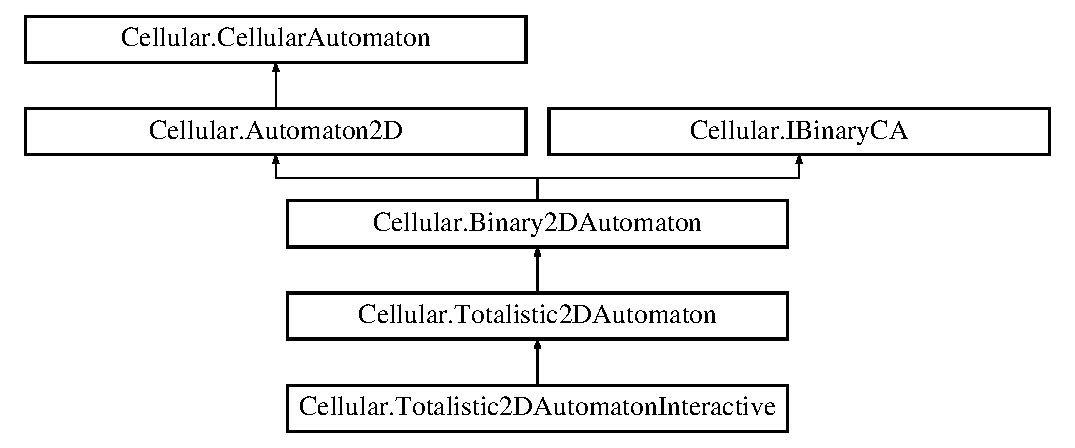
\includegraphics[height=5.000000cm]{class_cellular_1_1_totalistic2_d_automaton}
\end{center}
\end{figure}
\subsection*{Public Member Functions}
\begin{DoxyCompactItemize}
\item 
\hyperlink{class_cellular_1_1_totalistic2_d_automaton_a4c7a751baa03c7caf2040d07bb772e91}{Totalistic2\+D\+Automaton} (bool\mbox{[}$\,$\mbox{]} \hyperlink{class_cellular_1_1_totalistic2_d_automaton_a4752e3402c58243f7f342e21ddad3b05}{rule\+Live}, bool\mbox{[}$\,$\mbox{]} rule\+Dead, int \hyperlink{class_cellular_1_1_automaton2_d_a1e9e5ec637c747a859c346839c90d174}{width}, int height, string specific\+Name=null)
\begin{DoxyCompactList}\small\item\em Creates a new totalistic 2\+D automaton of given ruleset with given initial state. \end{DoxyCompactList}\item 
\hyperlink{class_cellular_1_1_totalistic2_d_automaton_a706f4c765a54fef6003e6e208a073a1c}{Totalistic2\+D\+Automaton} (bool\mbox{[}$\,$\mbox{]} \hyperlink{class_cellular_1_1_totalistic2_d_automaton_a4752e3402c58243f7f342e21ddad3b05}{rule\+Live}, bool\mbox{[}$\,$\mbox{]} rule\+Dead, Bit\+Array\mbox{[}$\,$\mbox{]} initial\+State, string specific\+Name=null)
\begin{DoxyCompactList}\small\item\em Creates a new totalistic 2\+D automaton of given ruleset with given initial state. \end{DoxyCompactList}\item 
override void \hyperlink{class_cellular_1_1_totalistic2_d_automaton_a7f85cac5420f67a936cbd4cef33c4abc}{Step} ()
\begin{DoxyCompactList}\small\item\em Performs one step of the cellular automaton. Always calls {\ttfamily \hyperlink{class_cellular_1_1_cellular_automaton_aa70848d58015575974bc875ac5a89ae7}{Cellular\+Automaton.\+Step()}}. \end{DoxyCompactList}\item 
override object \hyperlink{class_cellular_1_1_totalistic2_d_automaton_ae78cf4c3f8245adf64ec9a173330804f}{Clone} ()
\begin{DoxyCompactList}\small\item\em Creates an appropriate copy of the C\+A. Its type and the specific rule are always preserved. However, the time (number of steps executed on the specific instance) is set back to 0. \end{DoxyCompactList}\item 
override string \hyperlink{class_cellular_1_1_totalistic2_d_automaton_aa009c674cd109fa70173e9893f6d3b09}{Tell\+Type} ()
\begin{DoxyCompactList}\small\item\em Announces the runtime type of the C\+A including info about its rule. It serves for debugging purposes. \end{DoxyCompactList}\end{DoxyCompactItemize}
\subsection*{Static Public Member Functions}
\begin{DoxyCompactItemize}
\item 
static \hyperlink{class_cellular_1_1_totalistic2_d_automaton}{Totalistic2\+D\+Automaton} \hyperlink{class_cellular_1_1_totalistic2_d_automaton_a76eeb87d529b320437eebbf664acf013}{Create\+Game\+Of\+Life} (int \hyperlink{class_cellular_1_1_automaton2_d_a1e9e5ec637c747a859c346839c90d174}{width}, int height)
\item 
static \hyperlink{class_cellular_1_1_totalistic2_d_automaton}{Totalistic2\+D\+Automaton} \hyperlink{class_cellular_1_1_totalistic2_d_automaton_aa8227b8be752f1c0e19f5cc6d605a011}{Create\+Game\+Of\+Life} (Bit\+Array\mbox{[}$\,$\mbox{]} initial\+State)
\item 
static \hyperlink{class_cellular_1_1_totalistic2_d_automaton}{Totalistic2\+D\+Automaton} \hyperlink{class_cellular_1_1_totalistic2_d_automaton_a79ed2d655e37829d26a9eed7974e726f}{Create\+Amoeba\+Universe} (int \hyperlink{class_cellular_1_1_automaton2_d_a1e9e5ec637c747a859c346839c90d174}{width}, int height)
\item 
static \hyperlink{class_cellular_1_1_totalistic2_d_automaton}{Totalistic2\+D\+Automaton} \hyperlink{class_cellular_1_1_totalistic2_d_automaton_a34a59a60c4a12e0b7904b37666385512}{Create\+Amoeba\+Universe} (Bit\+Array\mbox{[}$\,$\mbox{]} initial\+State)
\item 
static \hyperlink{class_cellular_1_1_totalistic2_d_automaton}{Totalistic2\+D\+Automaton} \hyperlink{class_cellular_1_1_totalistic2_d_automaton_a9f5a2308bc2b17ee7a9c779608e505ba}{Create\+Replicator\+Universe} (int \hyperlink{class_cellular_1_1_automaton2_d_a1e9e5ec637c747a859c346839c90d174}{width}, int height)
\item 
static \hyperlink{class_cellular_1_1_totalistic2_d_automaton}{Totalistic2\+D\+Automaton} \hyperlink{class_cellular_1_1_totalistic2_d_automaton_a0d8bbe04fcb603d8ff614864e39c386d}{Create\+Replicator\+Universe} (Bit\+Array\mbox{[}$\,$\mbox{]} initial\+State)
\end{DoxyCompactItemize}
\subsection*{Protected Member Functions}
\begin{DoxyCompactItemize}
\item 
override \hyperlink{interface_cellular_1_1_i_binary_c_a}{I\+Binary\+C\+A} \hyperlink{class_cellular_1_1_totalistic2_d_automaton_ad5cc3f46a556aa1b1c99bdfa92f5ba1d}{clone\+Template} (Bit\+Array\mbox{[}$\,$\mbox{]} new\+Instance\+State)
\end{DoxyCompactItemize}
\subsection*{Protected Attributes}
\begin{DoxyCompactItemize}
\item 
bool\mbox{[}$\,$\mbox{]} \hyperlink{class_cellular_1_1_totalistic2_d_automaton_a4752e3402c58243f7f342e21ddad3b05}{rule\+Live}
\item 
const string \hyperlink{class_cellular_1_1_totalistic2_d_automaton_a925e29c85ea53754a86864aa9b2e27f9}{descr\+Game\+Of\+Life} = \char`\"{}Game of Life\char`\"{}
\item 
const string \hyperlink{class_cellular_1_1_totalistic2_d_automaton_a0acaeddabe1e121966d99d9144eb3220}{descr\+Amoeba\+Universe} = \char`\"{}Amoeba Universe\char`\"{}
\item 
const string \hyperlink{class_cellular_1_1_totalistic2_d_automaton_ab93b5f3ae4587498fcccab5a77992ab9}{descr\+Replicator\+Universe} = \char`\"{}Replicator Universe\char`\"{}
\end{DoxyCompactItemize}
\subsection*{Static Protected Attributes}
\begin{DoxyCompactItemize}
\item 
static readonly bool\mbox{[}$\,$\mbox{]} \hyperlink{class_cellular_1_1_totalistic2_d_automaton_a4633d221a98d2f36cc876f5a08c61f1e}{live\+Game\+Of\+Life} = \{ false, false, true, true, false, false, false, false, false \}
\item 
static readonly bool\mbox{[}$\,$\mbox{]} \hyperlink{class_cellular_1_1_totalistic2_d_automaton_aa4888d1ead2dfcdb1c90c79485aed255}{dead\+Game\+Of\+Life} = \{ false, false, false, true, false, false, false, false, false \}
\item 
static readonly bool\mbox{[}$\,$\mbox{]} \hyperlink{class_cellular_1_1_totalistic2_d_automaton_a69f67fbf81c8a2c5a3700c4f9b55c596}{live\+Amoeba\+Universe} = \{ false, true, false, true, false, true, false, false, true \}
\item 
static readonly bool\mbox{[}$\,$\mbox{]} \hyperlink{class_cellular_1_1_totalistic2_d_automaton_a5b2dd1d361797410beda7ea765b40c31}{dead\+Amoeba\+Universe} = \{ false, false, false, true, false, true, false, true, false \}
\item 
static readonly bool\mbox{[}$\,$\mbox{]} \hyperlink{class_cellular_1_1_totalistic2_d_automaton_abb59a96261e32abc500ce4c7db88cdd6}{live\+Replicator\+Universe} = \{ false, true, false, true, false, true, false, true, false \}
\item 
static readonly bool\mbox{[}$\,$\mbox{]} \hyperlink{class_cellular_1_1_totalistic2_d_automaton_a195a2bf20843bbc0980979ef889170d3}{dead\+Replicator\+Universe} = \{ false, true, false, true, false, true, false, true, false \}
\end{DoxyCompactItemize}


\subsection{Detailed Description}
Class representing a totalistic 2\+D automaton that uses Moore Neighborhood. 



Definition at line 9 of file Totalistic2\+D\+Automaton.\+cs.



\subsection{Constructor \& Destructor Documentation}
\hypertarget{class_cellular_1_1_totalistic2_d_automaton_a4c7a751baa03c7caf2040d07bb772e91}{}\index{Cellular\+::\+Totalistic2\+D\+Automaton@{Cellular\+::\+Totalistic2\+D\+Automaton}!Totalistic2\+D\+Automaton@{Totalistic2\+D\+Automaton}}
\index{Totalistic2\+D\+Automaton@{Totalistic2\+D\+Automaton}!Cellular\+::\+Totalistic2\+D\+Automaton@{Cellular\+::\+Totalistic2\+D\+Automaton}}
\subsubsection[{Totalistic2\+D\+Automaton(bool[] rule\+Live, bool[] rule\+Dead, int width, int height, string specific\+Name=null)}]{\setlength{\rightskip}{0pt plus 5cm}Cellular.\+Totalistic2\+D\+Automaton.\+Totalistic2\+D\+Automaton (
\begin{DoxyParamCaption}
\item[{bool\mbox{[}$\,$\mbox{]}}]{rule\+Live, }
\item[{bool\mbox{[}$\,$\mbox{]}}]{rule\+Dead, }
\item[{int}]{width, }
\item[{int}]{height, }
\item[{string}]{specific\+Name = {\ttfamily null}}
\end{DoxyParamCaption}
)}\label{class_cellular_1_1_totalistic2_d_automaton_a4c7a751baa03c7caf2040d07bb772e91}


Creates a new totalistic 2\+D automaton of given ruleset with given initial state. 


\begin{DoxyParams}{Parameters}
{\em rule\+Live} & Array that must contain 9 logical values. The value in {\ttfamily rule\+Live\mbox{[}i\mbox{]}} says what happens to a living cell when it has exactly i neighbours alive.\\
\hline
{\em rule\+Dead} & Array that must contain 9 logical values. The value in {\ttfamily rule\+Dead\mbox{[}i\mbox{]}} says what happens to a dead cell when it has exactly i neighbours alive.\\
\hline
{\em width} & The width of the new C\+A (length of rows).\\
\hline
{\em height} & The height of the new C\+A (number of rows).\\
\hline
{\em rnd} & Pseudo\+R\+N\+G instance that will be used to generate the original state.\\
\hline
\end{DoxyParams}


Definition at line 24 of file Totalistic2\+D\+Automaton.\+cs.

\hypertarget{class_cellular_1_1_totalistic2_d_automaton_a706f4c765a54fef6003e6e208a073a1c}{}\index{Cellular\+::\+Totalistic2\+D\+Automaton@{Cellular\+::\+Totalistic2\+D\+Automaton}!Totalistic2\+D\+Automaton@{Totalistic2\+D\+Automaton}}
\index{Totalistic2\+D\+Automaton@{Totalistic2\+D\+Automaton}!Cellular\+::\+Totalistic2\+D\+Automaton@{Cellular\+::\+Totalistic2\+D\+Automaton}}
\subsubsection[{Totalistic2\+D\+Automaton(bool[] rule\+Live, bool[] rule\+Dead, Bit\+Array[] initial\+State, string specific\+Name=null)}]{\setlength{\rightskip}{0pt plus 5cm}Cellular.\+Totalistic2\+D\+Automaton.\+Totalistic2\+D\+Automaton (
\begin{DoxyParamCaption}
\item[{bool\mbox{[}$\,$\mbox{]}}]{rule\+Live, }
\item[{bool\mbox{[}$\,$\mbox{]}}]{rule\+Dead, }
\item[{Bit\+Array\mbox{[}$\,$\mbox{]}}]{initial\+State, }
\item[{string}]{specific\+Name = {\ttfamily null}}
\end{DoxyParamCaption}
)}\label{class_cellular_1_1_totalistic2_d_automaton_a706f4c765a54fef6003e6e208a073a1c}


Creates a new totalistic 2\+D automaton of given ruleset with given initial state. 


\begin{DoxyParams}{Parameters}
{\em rule\+Live} & Array that must contain 9 logical values. The value in {\ttfamily rule\+Live\mbox{[}i\mbox{]}} says what happens to a living cell when it has exactly i neighbours alive.\\
\hline
{\em rule\+Dead} & Array that must contain 9 logical values. The value in {\ttfamily rule\+Dead\mbox{[}i\mbox{]}} says what happens to a dead cell when it has exactly i neighbours alive.\\
\hline
{\em initial\+State} & An array of {\ttfamily Bit\+Array}s describing the initial state of the C\+A. This also determines the size (width, height) of the new C\+A.\\
\hline
\end{DoxyParams}


Definition at line 40 of file Totalistic2\+D\+Automaton.\+cs.



\subsection{Member Function Documentation}
\hypertarget{class_cellular_1_1_totalistic2_d_automaton_ae78cf4c3f8245adf64ec9a173330804f}{}\index{Cellular\+::\+Totalistic2\+D\+Automaton@{Cellular\+::\+Totalistic2\+D\+Automaton}!Clone@{Clone}}
\index{Clone@{Clone}!Cellular\+::\+Totalistic2\+D\+Automaton@{Cellular\+::\+Totalistic2\+D\+Automaton}}
\subsubsection[{Clone()}]{\setlength{\rightskip}{0pt plus 5cm}override object Cellular.\+Totalistic2\+D\+Automaton.\+Clone (
\begin{DoxyParamCaption}
{}
\end{DoxyParamCaption}
)\hspace{0.3cm}{\ttfamily [virtual]}}\label{class_cellular_1_1_totalistic2_d_automaton_ae78cf4c3f8245adf64ec9a173330804f}


Creates an appropriate copy of the C\+A. Its type and the specific rule are always preserved. However, the time (number of steps executed on the specific instance) is set back to 0. 

\begin{DoxyReturn}{Returns}
A copy of the {\ttfamily \hyperlink{class_cellular_1_1_cellular_automaton}{Cellular\+Automaton}} as {\ttfamily System.\+Object}
\end{DoxyReturn}


Implements \hyperlink{class_cellular_1_1_cellular_automaton_affd487b397cdbbbb1982815bbcd8e7d3}{Cellular.\+Cellular\+Automaton}.



Definition at line 252 of file Totalistic2\+D\+Automaton.\+cs.

\hypertarget{class_cellular_1_1_totalistic2_d_automaton_ad5cc3f46a556aa1b1c99bdfa92f5ba1d}{}\index{Cellular\+::\+Totalistic2\+D\+Automaton@{Cellular\+::\+Totalistic2\+D\+Automaton}!clone\+Template@{clone\+Template}}
\index{clone\+Template@{clone\+Template}!Cellular\+::\+Totalistic2\+D\+Automaton@{Cellular\+::\+Totalistic2\+D\+Automaton}}
\subsubsection[{clone\+Template(\+Bit\+Array[] new\+Instance\+State)}]{\setlength{\rightskip}{0pt plus 5cm}override {\bf I\+Binary\+C\+A} Cellular.\+Totalistic2\+D\+Automaton.\+clone\+Template (
\begin{DoxyParamCaption}
\item[{Bit\+Array\mbox{[}$\,$\mbox{]}}]{new\+Instance\+State}
\end{DoxyParamCaption}
)\hspace{0.3cm}{\ttfamily [protected]}, {\ttfamily [virtual]}}\label{class_cellular_1_1_totalistic2_d_automaton_ad5cc3f46a556aa1b1c99bdfa92f5ba1d}


Implements \hyperlink{class_cellular_1_1_binary2_d_automaton_ad2d31668c7b8f8e959575e03b995273f}{Cellular.\+Binary2\+D\+Automaton}.



Definition at line 257 of file Totalistic2\+D\+Automaton.\+cs.

\hypertarget{class_cellular_1_1_totalistic2_d_automaton_a79ed2d655e37829d26a9eed7974e726f}{}\index{Cellular\+::\+Totalistic2\+D\+Automaton@{Cellular\+::\+Totalistic2\+D\+Automaton}!Create\+Amoeba\+Universe@{Create\+Amoeba\+Universe}}
\index{Create\+Amoeba\+Universe@{Create\+Amoeba\+Universe}!Cellular\+::\+Totalistic2\+D\+Automaton@{Cellular\+::\+Totalistic2\+D\+Automaton}}
\subsubsection[{Create\+Amoeba\+Universe(int width, int height)}]{\setlength{\rightskip}{0pt plus 5cm}static {\bf Totalistic2\+D\+Automaton} Cellular.\+Totalistic2\+D\+Automaton.\+Create\+Amoeba\+Universe (
\begin{DoxyParamCaption}
\item[{int}]{width, }
\item[{int}]{height}
\end{DoxyParamCaption}
)\hspace{0.3cm}{\ttfamily [static]}}\label{class_cellular_1_1_totalistic2_d_automaton_a79ed2d655e37829d26a9eed7974e726f}


Definition at line 77 of file Totalistic2\+D\+Automaton.\+cs.

\hypertarget{class_cellular_1_1_totalistic2_d_automaton_a34a59a60c4a12e0b7904b37666385512}{}\index{Cellular\+::\+Totalistic2\+D\+Automaton@{Cellular\+::\+Totalistic2\+D\+Automaton}!Create\+Amoeba\+Universe@{Create\+Amoeba\+Universe}}
\index{Create\+Amoeba\+Universe@{Create\+Amoeba\+Universe}!Cellular\+::\+Totalistic2\+D\+Automaton@{Cellular\+::\+Totalistic2\+D\+Automaton}}
\subsubsection[{Create\+Amoeba\+Universe(\+Bit\+Array[] initial\+State)}]{\setlength{\rightskip}{0pt plus 5cm}static {\bf Totalistic2\+D\+Automaton} Cellular.\+Totalistic2\+D\+Automaton.\+Create\+Amoeba\+Universe (
\begin{DoxyParamCaption}
\item[{Bit\+Array\mbox{[}$\,$\mbox{]}}]{initial\+State}
\end{DoxyParamCaption}
)\hspace{0.3cm}{\ttfamily [static]}}\label{class_cellular_1_1_totalistic2_d_automaton_a34a59a60c4a12e0b7904b37666385512}


Definition at line 82 of file Totalistic2\+D\+Automaton.\+cs.

\hypertarget{class_cellular_1_1_totalistic2_d_automaton_a76eeb87d529b320437eebbf664acf013}{}\index{Cellular\+::\+Totalistic2\+D\+Automaton@{Cellular\+::\+Totalistic2\+D\+Automaton}!Create\+Game\+Of\+Life@{Create\+Game\+Of\+Life}}
\index{Create\+Game\+Of\+Life@{Create\+Game\+Of\+Life}!Cellular\+::\+Totalistic2\+D\+Automaton@{Cellular\+::\+Totalistic2\+D\+Automaton}}
\subsubsection[{Create\+Game\+Of\+Life(int width, int height)}]{\setlength{\rightskip}{0pt plus 5cm}static {\bf Totalistic2\+D\+Automaton} Cellular.\+Totalistic2\+D\+Automaton.\+Create\+Game\+Of\+Life (
\begin{DoxyParamCaption}
\item[{int}]{width, }
\item[{int}]{height}
\end{DoxyParamCaption}
)\hspace{0.3cm}{\ttfamily [static]}}\label{class_cellular_1_1_totalistic2_d_automaton_a76eeb87d529b320437eebbf664acf013}


Definition at line 62 of file Totalistic2\+D\+Automaton.\+cs.

\hypertarget{class_cellular_1_1_totalistic2_d_automaton_aa8227b8be752f1c0e19f5cc6d605a011}{}\index{Cellular\+::\+Totalistic2\+D\+Automaton@{Cellular\+::\+Totalistic2\+D\+Automaton}!Create\+Game\+Of\+Life@{Create\+Game\+Of\+Life}}
\index{Create\+Game\+Of\+Life@{Create\+Game\+Of\+Life}!Cellular\+::\+Totalistic2\+D\+Automaton@{Cellular\+::\+Totalistic2\+D\+Automaton}}
\subsubsection[{Create\+Game\+Of\+Life(\+Bit\+Array[] initial\+State)}]{\setlength{\rightskip}{0pt plus 5cm}static {\bf Totalistic2\+D\+Automaton} Cellular.\+Totalistic2\+D\+Automaton.\+Create\+Game\+Of\+Life (
\begin{DoxyParamCaption}
\item[{Bit\+Array\mbox{[}$\,$\mbox{]}}]{initial\+State}
\end{DoxyParamCaption}
)\hspace{0.3cm}{\ttfamily [static]}}\label{class_cellular_1_1_totalistic2_d_automaton_aa8227b8be752f1c0e19f5cc6d605a011}


Definition at line 67 of file Totalistic2\+D\+Automaton.\+cs.

\hypertarget{class_cellular_1_1_totalistic2_d_automaton_a9f5a2308bc2b17ee7a9c779608e505ba}{}\index{Cellular\+::\+Totalistic2\+D\+Automaton@{Cellular\+::\+Totalistic2\+D\+Automaton}!Create\+Replicator\+Universe@{Create\+Replicator\+Universe}}
\index{Create\+Replicator\+Universe@{Create\+Replicator\+Universe}!Cellular\+::\+Totalistic2\+D\+Automaton@{Cellular\+::\+Totalistic2\+D\+Automaton}}
\subsubsection[{Create\+Replicator\+Universe(int width, int height)}]{\setlength{\rightskip}{0pt plus 5cm}static {\bf Totalistic2\+D\+Automaton} Cellular.\+Totalistic2\+D\+Automaton.\+Create\+Replicator\+Universe (
\begin{DoxyParamCaption}
\item[{int}]{width, }
\item[{int}]{height}
\end{DoxyParamCaption}
)\hspace{0.3cm}{\ttfamily [static]}}\label{class_cellular_1_1_totalistic2_d_automaton_a9f5a2308bc2b17ee7a9c779608e505ba}


Definition at line 92 of file Totalistic2\+D\+Automaton.\+cs.

\hypertarget{class_cellular_1_1_totalistic2_d_automaton_a0d8bbe04fcb603d8ff614864e39c386d}{}\index{Cellular\+::\+Totalistic2\+D\+Automaton@{Cellular\+::\+Totalistic2\+D\+Automaton}!Create\+Replicator\+Universe@{Create\+Replicator\+Universe}}
\index{Create\+Replicator\+Universe@{Create\+Replicator\+Universe}!Cellular\+::\+Totalistic2\+D\+Automaton@{Cellular\+::\+Totalistic2\+D\+Automaton}}
\subsubsection[{Create\+Replicator\+Universe(\+Bit\+Array[] initial\+State)}]{\setlength{\rightskip}{0pt plus 5cm}static {\bf Totalistic2\+D\+Automaton} Cellular.\+Totalistic2\+D\+Automaton.\+Create\+Replicator\+Universe (
\begin{DoxyParamCaption}
\item[{Bit\+Array\mbox{[}$\,$\mbox{]}}]{initial\+State}
\end{DoxyParamCaption}
)\hspace{0.3cm}{\ttfamily [static]}}\label{class_cellular_1_1_totalistic2_d_automaton_a0d8bbe04fcb603d8ff614864e39c386d}


Definition at line 97 of file Totalistic2\+D\+Automaton.\+cs.

\hypertarget{class_cellular_1_1_totalistic2_d_automaton_a7f85cac5420f67a936cbd4cef33c4abc}{}\index{Cellular\+::\+Totalistic2\+D\+Automaton@{Cellular\+::\+Totalistic2\+D\+Automaton}!Step@{Step}}
\index{Step@{Step}!Cellular\+::\+Totalistic2\+D\+Automaton@{Cellular\+::\+Totalistic2\+D\+Automaton}}
\subsubsection[{Step()}]{\setlength{\rightskip}{0pt plus 5cm}override void Cellular.\+Totalistic2\+D\+Automaton.\+Step (
\begin{DoxyParamCaption}
{}
\end{DoxyParamCaption}
)}\label{class_cellular_1_1_totalistic2_d_automaton_a7f85cac5420f67a936cbd4cef33c4abc}


Performs one step of the cellular automaton. Always calls {\ttfamily \hyperlink{class_cellular_1_1_cellular_automaton_aa70848d58015575974bc875ac5a89ae7}{Cellular\+Automaton.\+Step()}}. 



Implements \hyperlink{interface_cellular_1_1_i_binary_c_a_a6a04c7374538c49df07efa176e0dd3c3}{Cellular.\+I\+Binary\+C\+A}.



Definition at line 102 of file Totalistic2\+D\+Automaton.\+cs.

\hypertarget{class_cellular_1_1_totalistic2_d_automaton_aa009c674cd109fa70173e9893f6d3b09}{}\index{Cellular\+::\+Totalistic2\+D\+Automaton@{Cellular\+::\+Totalistic2\+D\+Automaton}!Tell\+Type@{Tell\+Type}}
\index{Tell\+Type@{Tell\+Type}!Cellular\+::\+Totalistic2\+D\+Automaton@{Cellular\+::\+Totalistic2\+D\+Automaton}}
\subsubsection[{Tell\+Type()}]{\setlength{\rightskip}{0pt plus 5cm}override string Cellular.\+Totalistic2\+D\+Automaton.\+Tell\+Type (
\begin{DoxyParamCaption}
{}
\end{DoxyParamCaption}
)}\label{class_cellular_1_1_totalistic2_d_automaton_aa009c674cd109fa70173e9893f6d3b09}


Announces the runtime type of the C\+A including info about its rule. It serves for debugging purposes. 

\begin{DoxyReturn}{Returns}
The same string as calling {\ttfamily \hyperlink{class_cellular_1_1_cellular_automaton_abe4b92fd405530c8a08cc07a3a19fff4}{Cellular\+Automaton.\+Tell\+Type()}}.
\end{DoxyReturn}


Implements \hyperlink{interface_cellular_1_1_i_binary_c_a_aa67feabf5d1513aa74076d255c661948}{Cellular.\+I\+Binary\+C\+A}.



Definition at line 262 of file Totalistic2\+D\+Automaton.\+cs.



\subsection{Member Data Documentation}
\hypertarget{class_cellular_1_1_totalistic2_d_automaton_a5b2dd1d361797410beda7ea765b40c31}{}\index{Cellular\+::\+Totalistic2\+D\+Automaton@{Cellular\+::\+Totalistic2\+D\+Automaton}!dead\+Amoeba\+Universe@{dead\+Amoeba\+Universe}}
\index{dead\+Amoeba\+Universe@{dead\+Amoeba\+Universe}!Cellular\+::\+Totalistic2\+D\+Automaton@{Cellular\+::\+Totalistic2\+D\+Automaton}}
\subsubsection[{dead\+Amoeba\+Universe}]{\setlength{\rightskip}{0pt plus 5cm}readonly bool \mbox{[}$\,$\mbox{]} Cellular.\+Totalistic2\+D\+Automaton.\+dead\+Amoeba\+Universe = \{ false, false, false, true, false, true, false, true, false \}\hspace{0.3cm}{\ttfamily [static]}, {\ttfamily [protected]}}\label{class_cellular_1_1_totalistic2_d_automaton_a5b2dd1d361797410beda7ea765b40c31}


Definition at line 74 of file Totalistic2\+D\+Automaton.\+cs.

\hypertarget{class_cellular_1_1_totalistic2_d_automaton_aa4888d1ead2dfcdb1c90c79485aed255}{}\index{Cellular\+::\+Totalistic2\+D\+Automaton@{Cellular\+::\+Totalistic2\+D\+Automaton}!dead\+Game\+Of\+Life@{dead\+Game\+Of\+Life}}
\index{dead\+Game\+Of\+Life@{dead\+Game\+Of\+Life}!Cellular\+::\+Totalistic2\+D\+Automaton@{Cellular\+::\+Totalistic2\+D\+Automaton}}
\subsubsection[{dead\+Game\+Of\+Life}]{\setlength{\rightskip}{0pt plus 5cm}readonly bool \mbox{[}$\,$\mbox{]} Cellular.\+Totalistic2\+D\+Automaton.\+dead\+Game\+Of\+Life = \{ false, false, false, true, false, false, false, false, false \}\hspace{0.3cm}{\ttfamily [static]}, {\ttfamily [protected]}}\label{class_cellular_1_1_totalistic2_d_automaton_aa4888d1ead2dfcdb1c90c79485aed255}


Definition at line 59 of file Totalistic2\+D\+Automaton.\+cs.

\hypertarget{class_cellular_1_1_totalistic2_d_automaton_a195a2bf20843bbc0980979ef889170d3}{}\index{Cellular\+::\+Totalistic2\+D\+Automaton@{Cellular\+::\+Totalistic2\+D\+Automaton}!dead\+Replicator\+Universe@{dead\+Replicator\+Universe}}
\index{dead\+Replicator\+Universe@{dead\+Replicator\+Universe}!Cellular\+::\+Totalistic2\+D\+Automaton@{Cellular\+::\+Totalistic2\+D\+Automaton}}
\subsubsection[{dead\+Replicator\+Universe}]{\setlength{\rightskip}{0pt plus 5cm}readonly bool \mbox{[}$\,$\mbox{]} Cellular.\+Totalistic2\+D\+Automaton.\+dead\+Replicator\+Universe = \{ false, true, false, true, false, true, false, true, false \}\hspace{0.3cm}{\ttfamily [static]}, {\ttfamily [protected]}}\label{class_cellular_1_1_totalistic2_d_automaton_a195a2bf20843bbc0980979ef889170d3}


Definition at line 89 of file Totalistic2\+D\+Automaton.\+cs.

\hypertarget{class_cellular_1_1_totalistic2_d_automaton_a0acaeddabe1e121966d99d9144eb3220}{}\index{Cellular\+::\+Totalistic2\+D\+Automaton@{Cellular\+::\+Totalistic2\+D\+Automaton}!descr\+Amoeba\+Universe@{descr\+Amoeba\+Universe}}
\index{descr\+Amoeba\+Universe@{descr\+Amoeba\+Universe}!Cellular\+::\+Totalistic2\+D\+Automaton@{Cellular\+::\+Totalistic2\+D\+Automaton}}
\subsubsection[{descr\+Amoeba\+Universe}]{\setlength{\rightskip}{0pt plus 5cm}const string Cellular.\+Totalistic2\+D\+Automaton.\+descr\+Amoeba\+Universe = \char`\"{}Amoeba Universe\char`\"{}\hspace{0.3cm}{\ttfamily [protected]}}\label{class_cellular_1_1_totalistic2_d_automaton_a0acaeddabe1e121966d99d9144eb3220}


Definition at line 75 of file Totalistic2\+D\+Automaton.\+cs.

\hypertarget{class_cellular_1_1_totalistic2_d_automaton_a925e29c85ea53754a86864aa9b2e27f9}{}\index{Cellular\+::\+Totalistic2\+D\+Automaton@{Cellular\+::\+Totalistic2\+D\+Automaton}!descr\+Game\+Of\+Life@{descr\+Game\+Of\+Life}}
\index{descr\+Game\+Of\+Life@{descr\+Game\+Of\+Life}!Cellular\+::\+Totalistic2\+D\+Automaton@{Cellular\+::\+Totalistic2\+D\+Automaton}}
\subsubsection[{descr\+Game\+Of\+Life}]{\setlength{\rightskip}{0pt plus 5cm}const string Cellular.\+Totalistic2\+D\+Automaton.\+descr\+Game\+Of\+Life = \char`\"{}Game of Life\char`\"{}\hspace{0.3cm}{\ttfamily [protected]}}\label{class_cellular_1_1_totalistic2_d_automaton_a925e29c85ea53754a86864aa9b2e27f9}


Definition at line 60 of file Totalistic2\+D\+Automaton.\+cs.

\hypertarget{class_cellular_1_1_totalistic2_d_automaton_ab93b5f3ae4587498fcccab5a77992ab9}{}\index{Cellular\+::\+Totalistic2\+D\+Automaton@{Cellular\+::\+Totalistic2\+D\+Automaton}!descr\+Replicator\+Universe@{descr\+Replicator\+Universe}}
\index{descr\+Replicator\+Universe@{descr\+Replicator\+Universe}!Cellular\+::\+Totalistic2\+D\+Automaton@{Cellular\+::\+Totalistic2\+D\+Automaton}}
\subsubsection[{descr\+Replicator\+Universe}]{\setlength{\rightskip}{0pt plus 5cm}const string Cellular.\+Totalistic2\+D\+Automaton.\+descr\+Replicator\+Universe = \char`\"{}Replicator Universe\char`\"{}\hspace{0.3cm}{\ttfamily [protected]}}\label{class_cellular_1_1_totalistic2_d_automaton_ab93b5f3ae4587498fcccab5a77992ab9}


Definition at line 90 of file Totalistic2\+D\+Automaton.\+cs.

\hypertarget{class_cellular_1_1_totalistic2_d_automaton_a69f67fbf81c8a2c5a3700c4f9b55c596}{}\index{Cellular\+::\+Totalistic2\+D\+Automaton@{Cellular\+::\+Totalistic2\+D\+Automaton}!live\+Amoeba\+Universe@{live\+Amoeba\+Universe}}
\index{live\+Amoeba\+Universe@{live\+Amoeba\+Universe}!Cellular\+::\+Totalistic2\+D\+Automaton@{Cellular\+::\+Totalistic2\+D\+Automaton}}
\subsubsection[{live\+Amoeba\+Universe}]{\setlength{\rightskip}{0pt plus 5cm}readonly bool \mbox{[}$\,$\mbox{]} Cellular.\+Totalistic2\+D\+Automaton.\+live\+Amoeba\+Universe = \{ false, true, false, true, false, true, false, false, true \}\hspace{0.3cm}{\ttfamily [static]}, {\ttfamily [protected]}}\label{class_cellular_1_1_totalistic2_d_automaton_a69f67fbf81c8a2c5a3700c4f9b55c596}


Definition at line 72 of file Totalistic2\+D\+Automaton.\+cs.

\hypertarget{class_cellular_1_1_totalistic2_d_automaton_a4633d221a98d2f36cc876f5a08c61f1e}{}\index{Cellular\+::\+Totalistic2\+D\+Automaton@{Cellular\+::\+Totalistic2\+D\+Automaton}!live\+Game\+Of\+Life@{live\+Game\+Of\+Life}}
\index{live\+Game\+Of\+Life@{live\+Game\+Of\+Life}!Cellular\+::\+Totalistic2\+D\+Automaton@{Cellular\+::\+Totalistic2\+D\+Automaton}}
\subsubsection[{live\+Game\+Of\+Life}]{\setlength{\rightskip}{0pt plus 5cm}readonly bool \mbox{[}$\,$\mbox{]} Cellular.\+Totalistic2\+D\+Automaton.\+live\+Game\+Of\+Life = \{ false, false, true, true, false, false, false, false, false \}\hspace{0.3cm}{\ttfamily [static]}, {\ttfamily [protected]}}\label{class_cellular_1_1_totalistic2_d_automaton_a4633d221a98d2f36cc876f5a08c61f1e}


Definition at line 57 of file Totalistic2\+D\+Automaton.\+cs.

\hypertarget{class_cellular_1_1_totalistic2_d_automaton_abb59a96261e32abc500ce4c7db88cdd6}{}\index{Cellular\+::\+Totalistic2\+D\+Automaton@{Cellular\+::\+Totalistic2\+D\+Automaton}!live\+Replicator\+Universe@{live\+Replicator\+Universe}}
\index{live\+Replicator\+Universe@{live\+Replicator\+Universe}!Cellular\+::\+Totalistic2\+D\+Automaton@{Cellular\+::\+Totalistic2\+D\+Automaton}}
\subsubsection[{live\+Replicator\+Universe}]{\setlength{\rightskip}{0pt plus 5cm}readonly bool \mbox{[}$\,$\mbox{]} Cellular.\+Totalistic2\+D\+Automaton.\+live\+Replicator\+Universe = \{ false, true, false, true, false, true, false, true, false \}\hspace{0.3cm}{\ttfamily [static]}, {\ttfamily [protected]}}\label{class_cellular_1_1_totalistic2_d_automaton_abb59a96261e32abc500ce4c7db88cdd6}


Definition at line 87 of file Totalistic2\+D\+Automaton.\+cs.

\hypertarget{class_cellular_1_1_totalistic2_d_automaton_a4752e3402c58243f7f342e21ddad3b05}{}\index{Cellular\+::\+Totalistic2\+D\+Automaton@{Cellular\+::\+Totalistic2\+D\+Automaton}!rule\+Live@{rule\+Live}}
\index{rule\+Live@{rule\+Live}!Cellular\+::\+Totalistic2\+D\+Automaton@{Cellular\+::\+Totalistic2\+D\+Automaton}}
\subsubsection[{rule\+Live}]{\setlength{\rightskip}{0pt plus 5cm}bool \mbox{[}$\,$\mbox{]} Cellular.\+Totalistic2\+D\+Automaton.\+rule\+Live\hspace{0.3cm}{\ttfamily [protected]}}\label{class_cellular_1_1_totalistic2_d_automaton_a4752e3402c58243f7f342e21ddad3b05}


Definition at line 11 of file Totalistic2\+D\+Automaton.\+cs.



The documentation for this class was generated from the following file\+:\begin{DoxyCompactItemize}
\item 
C\+:/\+Martin/\+M\+F\+F/\+\_\+baka/\+Martin\+Dvorak/\+Cellular/\hyperlink{_totalistic2_d_automaton_8cs}{Totalistic2\+D\+Automaton.\+cs}\end{DoxyCompactItemize}

\input{class_cellular_1_1_totalistic2_d_automaton_interactive}
\hypertarget{class_testing_1_1_totalistic_ternary_test}{}\section{Testing.\+Totalistic\+Ternary\+Test Class Reference}
\label{class_testing_1_1_totalistic_ternary_test}\index{Testing.\+Totalistic\+Ternary\+Test@{Testing.\+Totalistic\+Ternary\+Test}}


Simple demonstration of 1\+D ternary totalistic automata.  


\subsection*{Static Public Member Functions}
\begin{DoxyCompactItemize}
\item 
static void \hyperlink{class_testing_1_1_totalistic_ternary_test_a3ba8f77c71da1744625f2e3714dd9c1f}{Run\+Test} ()
\end{DoxyCompactItemize}


\subsection{Detailed Description}
Simple demonstration of 1\+D ternary totalistic automata. 



Definition at line 9 of file Totalistic\+Ternary\+Test.\+cs.



\subsection{Member Function Documentation}
\hypertarget{class_testing_1_1_totalistic_ternary_test_a3ba8f77c71da1744625f2e3714dd9c1f}{}\index{Testing\+::\+Totalistic\+Ternary\+Test@{Testing\+::\+Totalistic\+Ternary\+Test}!Run\+Test@{Run\+Test}}
\index{Run\+Test@{Run\+Test}!Testing\+::\+Totalistic\+Ternary\+Test@{Testing\+::\+Totalistic\+Ternary\+Test}}
\subsubsection[{Run\+Test()}]{\setlength{\rightskip}{0pt plus 5cm}static void Testing.\+Totalistic\+Ternary\+Test.\+Run\+Test (
\begin{DoxyParamCaption}
{}
\end{DoxyParamCaption}
)\hspace{0.3cm}{\ttfamily [static]}}\label{class_testing_1_1_totalistic_ternary_test_a3ba8f77c71da1744625f2e3714dd9c1f}


Definition at line 11 of file Totalistic\+Ternary\+Test.\+cs.



The documentation for this class was generated from the following file\+:\begin{DoxyCompactItemize}
\item 
C\+:/\+Martin/\+M\+F\+F/\+\_\+baka/\+Martin\+Dvorak/\+Testing/\hyperlink{_totalistic_ternary_test_8cs}{Totalistic\+Ternary\+Test.\+cs}\end{DoxyCompactItemize}

\hypertarget{class_cellular_1_1_utilities}{}\section{Cellular.\+Utilities Class Reference}
\label{class_cellular_1_1_utilities}\index{Cellular.\+Utilities@{Cellular.\+Utilities}}


Static class packing a group of utilities for working with C\+A.  


\subsection*{Classes}
\begin{DoxyCompactItemize}
\item 
class \hyperlink{class_cellular_1_1_utilities_1_1_all_binary_sequences}{All\+Binary\+Sequences}
\begin{DoxyCompactList}\small\item\em Class for enumerating all binary sequences of a given length. Starting from 00...00, ending at 11...11. \end{DoxyCompactList}\end{DoxyCompactItemize}
\subsection*{Static Public Member Functions}
\begin{DoxyCompactItemize}
\item 
static bool\mbox{[}$\,$\mbox{]} \hyperlink{class_cellular_1_1_utilities_a6f1fcc096938174c779453fb588cbfdb}{Uint\+Arr\+To\+Bool\+Arr} (uint\mbox{[}$\,$\mbox{]} input)
\begin{DoxyCompactList}\small\item\em Converts an array of {\ttfamily System.\+U\+Int32} into an array of {\ttfamily System.\+Boolean}. The input is treated as M\+S\+B-\/first. \end{DoxyCompactList}\item 
static Bit\+Array \hyperlink{class_cellular_1_1_utilities_a3e6d6ebde1b445f03d3c0b1a9c0274e6}{Uint\+Arr\+To\+Bit\+Arr} (uint\mbox{[}$\,$\mbox{]} input)
\begin{DoxyCompactList}\small\item\em Converts an array of {\ttfamily System.\+U\+Int32} into an array of {\ttfamily System.\+Collections.\+Bit\+Array}. The input is treated as M\+S\+B-\/first. \end{DoxyCompactList}\item 
static bool\mbox{[}$\,$\mbox{]} \hyperlink{class_cellular_1_1_utilities_a1c47a345afd4e991876f6ae6c4723591}{Bit\+Arr\+To\+Bool\+Arr} (Bit\+Array bit\+Array)
\item 
static long \hyperlink{class_cellular_1_1_utilities_a8ebd90cf7f8d6ce2235d26f9feeddfae}{Period\+Length\+Fast} (\hyperlink{class_cellular_1_1_cellular_automaton}{Cellular\+Automaton} C\+A, long limit, out long time)
\begin{DoxyCompactList}\small\item\em Calculates a period (number of steps between repetitions) of a C\+A. This method is fast, but unreliable! It gives only the lower estimate (because of hashing). \end{DoxyCompactList}\item 
static long \hyperlink{class_cellular_1_1_utilities_a7a43545f264bf30884c8486a14fb4f43}{Period\+Length\+Fast} (\hyperlink{class_cellular_1_1_cellular_automaton}{Cellular\+Automaton} C\+A)
\begin{DoxyCompactList}\small\item\em Calculates a period (number of steps between repetitions) of a C\+A. This method is fast, but unreliable! It gives only the lower estimate (because of hashing). \end{DoxyCompactList}\item 
static long \hyperlink{class_cellular_1_1_utilities_aa0b71d2f39b127f7078a35263adbfd55}{Period\+Length\+Slow} (\hyperlink{interface_cellular_1_1_i_binary_c_a}{I\+Binary\+C\+A} C\+A, long limit, out long time)
\begin{DoxyCompactList}\small\item\em Calculates a period (number of steps between repetitions) of a binary C\+A. This method is slower, but reliable. \end{DoxyCompactList}\item 
static bool\mbox{[}$\,$\mbox{]} \hyperlink{class_cellular_1_1_utilities_a3f20fa274e0db626d4052fe233f7a00f}{Random\+Bool\+Arr} (int length, Random rnd)
\begin{DoxyCompactList}\small\item\em Generates a random array of {\ttfamily System.\+Boolean} of given length. \end{DoxyCompactList}\item 
static bool\mbox{[}$\,$\mbox{]} \hyperlink{class_cellular_1_1_utilities_a069e9224bbd6f305d17e38d6290424cd}{Random\+Bool\+Arr} (int length)
\begin{DoxyCompactList}\small\item\em Generates a random array of {\ttfamily System.\+Boolean} of given length. The instance of Pseudo-\/random number generator is created locally, so this method is unsuitable for repeated use. \end{DoxyCompactList}\item 
static Bit\+Array \hyperlink{class_cellular_1_1_utilities_a887bbf207bece7f1bfa93d3d3fab547d}{Random\+Bit\+Arr} (int length, Random rnd)
\begin{DoxyCompactList}\small\item\em Generates a random array of {\ttfamily System.\+Collections.\+Bit\+Array} of given length. \end{DoxyCompactList}\item 
static Bit\+Array \hyperlink{class_cellular_1_1_utilities_a9cf5e2901915830e230c8affacfcec18}{Random\+Bit\+Arr} (int length)
\begin{DoxyCompactList}\small\item\em Generates a random array of {\ttfamily System.\+Collections.\+Bit\+Array} of given length. The instance of Pseudo-\/random number generator is created locally, so this method is unsuitable for repeated use. \end{DoxyCompactList}\end{DoxyCompactItemize}


\subsection{Detailed Description}
Static class packing a group of utilities for working with C\+A. 



Definition at line 11 of file Utilities.\+cs.



\subsection{Member Function Documentation}
\hypertarget{class_cellular_1_1_utilities_a1c47a345afd4e991876f6ae6c4723591}{}\index{Cellular\+::\+Utilities@{Cellular\+::\+Utilities}!Bit\+Arr\+To\+Bool\+Arr@{Bit\+Arr\+To\+Bool\+Arr}}
\index{Bit\+Arr\+To\+Bool\+Arr@{Bit\+Arr\+To\+Bool\+Arr}!Cellular\+::\+Utilities@{Cellular\+::\+Utilities}}
\subsubsection[{Bit\+Arr\+To\+Bool\+Arr(\+Bit\+Array bit\+Array)}]{\setlength{\rightskip}{0pt plus 5cm}static bool \mbox{[}$\,$\mbox{]} Cellular.\+Utilities.\+Bit\+Arr\+To\+Bool\+Arr (
\begin{DoxyParamCaption}
\item[{Bit\+Array}]{bit\+Array}
\end{DoxyParamCaption}
)\hspace{0.3cm}{\ttfamily [static]}}\label{class_cellular_1_1_utilities_a1c47a345afd4e991876f6ae6c4723591}


Definition at line 59 of file Utilities.\+cs.

\hypertarget{class_cellular_1_1_utilities_a8ebd90cf7f8d6ce2235d26f9feeddfae}{}\index{Cellular\+::\+Utilities@{Cellular\+::\+Utilities}!Period\+Length\+Fast@{Period\+Length\+Fast}}
\index{Period\+Length\+Fast@{Period\+Length\+Fast}!Cellular\+::\+Utilities@{Cellular\+::\+Utilities}}
\subsubsection[{Period\+Length\+Fast(\+Cellular\+Automaton C\+A, long limit, out long time)}]{\setlength{\rightskip}{0pt plus 5cm}static long Cellular.\+Utilities.\+Period\+Length\+Fast (
\begin{DoxyParamCaption}
\item[{{\bf Cellular\+Automaton}}]{C\+A, }
\item[{long}]{limit, }
\item[{out long}]{time}
\end{DoxyParamCaption}
)\hspace{0.3cm}{\ttfamily [static]}}\label{class_cellular_1_1_utilities_a8ebd90cf7f8d6ce2235d26f9feeddfae}


Calculates a period (number of steps between repetitions) of a C\+A. This method is fast, but unreliable! It gives only the lower estimate (because of hashing). 


\begin{DoxyParams}{Parameters}
{\em C\+A} & The examined cellular automaton. Don\textquotesingle{}t worry, this method won\textquotesingle{}t modify it.\\
\hline
{\em limit} & Number of steps that will be performed in no repetition is found earlier.\\
\hline
{\em time} & Output parameter telling the time of a first repetition (second occurence of the same state). It is the number of steps done since calling this method (not a real time, not a period length).\\
\hline
\end{DoxyParams}
\begin{DoxyReturn}{Returns}
If a period is found within the limit, it returns the length of the period. Otherwise, it returns -\/1.
\end{DoxyReturn}


Definition at line 79 of file Utilities.\+cs.

\hypertarget{class_cellular_1_1_utilities_a7a43545f264bf30884c8486a14fb4f43}{}\index{Cellular\+::\+Utilities@{Cellular\+::\+Utilities}!Period\+Length\+Fast@{Period\+Length\+Fast}}
\index{Period\+Length\+Fast@{Period\+Length\+Fast}!Cellular\+::\+Utilities@{Cellular\+::\+Utilities}}
\subsubsection[{Period\+Length\+Fast(\+Cellular\+Automaton C\+A)}]{\setlength{\rightskip}{0pt plus 5cm}static long Cellular.\+Utilities.\+Period\+Length\+Fast (
\begin{DoxyParamCaption}
\item[{{\bf Cellular\+Automaton}}]{C\+A}
\end{DoxyParamCaption}
)\hspace{0.3cm}{\ttfamily [static]}}\label{class_cellular_1_1_utilities_a7a43545f264bf30884c8486a14fb4f43}


Calculates a period (number of steps between repetitions) of a C\+A. This method is fast, but unreliable! It gives only the lower estimate (because of hashing). 


\begin{DoxyParams}{Parameters}
{\em C\+A} & The examined cellular automaton. Don\textquotesingle{}t worry, this method won\textquotesingle{}t modify it.\\
\hline
\end{DoxyParams}
\begin{DoxyReturn}{Returns}
If a period is found within 2$^\wedge$30 steps, it returns the length of the period. Otherwise, it returns -\/1.
\end{DoxyReturn}


Definition at line 106 of file Utilities.\+cs.

\hypertarget{class_cellular_1_1_utilities_aa0b71d2f39b127f7078a35263adbfd55}{}\index{Cellular\+::\+Utilities@{Cellular\+::\+Utilities}!Period\+Length\+Slow@{Period\+Length\+Slow}}
\index{Period\+Length\+Slow@{Period\+Length\+Slow}!Cellular\+::\+Utilities@{Cellular\+::\+Utilities}}
\subsubsection[{Period\+Length\+Slow(\+I\+Binary\+C\+A C\+A, long limit, out long time)}]{\setlength{\rightskip}{0pt plus 5cm}static long Cellular.\+Utilities.\+Period\+Length\+Slow (
\begin{DoxyParamCaption}
\item[{{\bf I\+Binary\+C\+A}}]{C\+A, }
\item[{long}]{limit, }
\item[{out long}]{time}
\end{DoxyParamCaption}
)\hspace{0.3cm}{\ttfamily [static]}}\label{class_cellular_1_1_utilities_aa0b71d2f39b127f7078a35263adbfd55}


Calculates a period (number of steps between repetitions) of a binary C\+A. This method is slower, but reliable. 


\begin{DoxyParams}{Parameters}
{\em C\+A} & The examined cellular automaton. Don\textquotesingle{}t worry, this method won\textquotesingle{}t modify it.\\
\hline
{\em limit} & Number of steps that will be performed in no repetition is found earlier.\\
\hline
{\em time} & Output parameter telling the time of a first repetition (second occurence of the same state). It is the number of steps done since calling this method (not a real time, not a period length).\\
\hline
\end{DoxyParams}
\begin{DoxyReturn}{Returns}
If a period is found within the limit, it returns the length of the period. Otherwise, it returns -\/1.
\end{DoxyReturn}


Definition at line 131 of file Utilities.\+cs.

\hypertarget{class_cellular_1_1_utilities_a887bbf207bece7f1bfa93d3d3fab547d}{}\index{Cellular\+::\+Utilities@{Cellular\+::\+Utilities}!Random\+Bit\+Arr@{Random\+Bit\+Arr}}
\index{Random\+Bit\+Arr@{Random\+Bit\+Arr}!Cellular\+::\+Utilities@{Cellular\+::\+Utilities}}
\subsubsection[{Random\+Bit\+Arr(int length, Random rnd)}]{\setlength{\rightskip}{0pt plus 5cm}static Bit\+Array Cellular.\+Utilities.\+Random\+Bit\+Arr (
\begin{DoxyParamCaption}
\item[{int}]{length, }
\item[{Random}]{rnd}
\end{DoxyParamCaption}
)\hspace{0.3cm}{\ttfamily [static]}}\label{class_cellular_1_1_utilities_a887bbf207bece7f1bfa93d3d3fab547d}


Generates a random array of {\ttfamily System.\+Collections.\+Bit\+Array} of given length. 


\begin{DoxyParams}{Parameters}
{\em length} & The size of the array.\\
\hline
{\em rnd} & Pseudo-\/random number generator instance.\\
\hline
\end{DoxyParams}
\begin{DoxyReturn}{Returns}
Random array.
\end{DoxyReturn}


Definition at line 199 of file Utilities.\+cs.

\hypertarget{class_cellular_1_1_utilities_a9cf5e2901915830e230c8affacfcec18}{}\index{Cellular\+::\+Utilities@{Cellular\+::\+Utilities}!Random\+Bit\+Arr@{Random\+Bit\+Arr}}
\index{Random\+Bit\+Arr@{Random\+Bit\+Arr}!Cellular\+::\+Utilities@{Cellular\+::\+Utilities}}
\subsubsection[{Random\+Bit\+Arr(int length)}]{\setlength{\rightskip}{0pt plus 5cm}static Bit\+Array Cellular.\+Utilities.\+Random\+Bit\+Arr (
\begin{DoxyParamCaption}
\item[{int}]{length}
\end{DoxyParamCaption}
)\hspace{0.3cm}{\ttfamily [static]}}\label{class_cellular_1_1_utilities_a9cf5e2901915830e230c8affacfcec18}


Generates a random array of {\ttfamily System.\+Collections.\+Bit\+Array} of given length. The instance of Pseudo-\/random number generator is created locally, so this method is unsuitable for repeated use. 


\begin{DoxyParams}{Parameters}
{\em length} & The size of the array.\\
\hline
\end{DoxyParams}
\begin{DoxyReturn}{Returns}
Random array.
\end{DoxyReturn}


Definition at line 215 of file Utilities.\+cs.

\hypertarget{class_cellular_1_1_utilities_a3f20fa274e0db626d4052fe233f7a00f}{}\index{Cellular\+::\+Utilities@{Cellular\+::\+Utilities}!Random\+Bool\+Arr@{Random\+Bool\+Arr}}
\index{Random\+Bool\+Arr@{Random\+Bool\+Arr}!Cellular\+::\+Utilities@{Cellular\+::\+Utilities}}
\subsubsection[{Random\+Bool\+Arr(int length, Random rnd)}]{\setlength{\rightskip}{0pt plus 5cm}static bool \mbox{[}$\,$\mbox{]} Cellular.\+Utilities.\+Random\+Bool\+Arr (
\begin{DoxyParamCaption}
\item[{int}]{length, }
\item[{Random}]{rnd}
\end{DoxyParamCaption}
)\hspace{0.3cm}{\ttfamily [static]}}\label{class_cellular_1_1_utilities_a3f20fa274e0db626d4052fe233f7a00f}


Generates a random array of {\ttfamily System.\+Boolean} of given length. 


\begin{DoxyParams}{Parameters}
{\em length} & The size of the array.\\
\hline
{\em rnd} & Pseudo-\/random number generator instance.\\
\hline
\end{DoxyParams}
\begin{DoxyReturn}{Returns}
Random array.
\end{DoxyReturn}


Definition at line 172 of file Utilities.\+cs.

\hypertarget{class_cellular_1_1_utilities_a069e9224bbd6f305d17e38d6290424cd}{}\index{Cellular\+::\+Utilities@{Cellular\+::\+Utilities}!Random\+Bool\+Arr@{Random\+Bool\+Arr}}
\index{Random\+Bool\+Arr@{Random\+Bool\+Arr}!Cellular\+::\+Utilities@{Cellular\+::\+Utilities}}
\subsubsection[{Random\+Bool\+Arr(int length)}]{\setlength{\rightskip}{0pt plus 5cm}static bool \mbox{[}$\,$\mbox{]} Cellular.\+Utilities.\+Random\+Bool\+Arr (
\begin{DoxyParamCaption}
\item[{int}]{length}
\end{DoxyParamCaption}
)\hspace{0.3cm}{\ttfamily [static]}}\label{class_cellular_1_1_utilities_a069e9224bbd6f305d17e38d6290424cd}


Generates a random array of {\ttfamily System.\+Boolean} of given length. The instance of Pseudo-\/random number generator is created locally, so this method is unsuitable for repeated use. 


\begin{DoxyParams}{Parameters}
{\em length} & The size of the array.\\
\hline
\end{DoxyParams}
\begin{DoxyReturn}{Returns}
Random array.
\end{DoxyReturn}


Definition at line 188 of file Utilities.\+cs.

\hypertarget{class_cellular_1_1_utilities_a3e6d6ebde1b445f03d3c0b1a9c0274e6}{}\index{Cellular\+::\+Utilities@{Cellular\+::\+Utilities}!Uint\+Arr\+To\+Bit\+Arr@{Uint\+Arr\+To\+Bit\+Arr}}
\index{Uint\+Arr\+To\+Bit\+Arr@{Uint\+Arr\+To\+Bit\+Arr}!Cellular\+::\+Utilities@{Cellular\+::\+Utilities}}
\subsubsection[{Uint\+Arr\+To\+Bit\+Arr(uint[] input)}]{\setlength{\rightskip}{0pt plus 5cm}static Bit\+Array Cellular.\+Utilities.\+Uint\+Arr\+To\+Bit\+Arr (
\begin{DoxyParamCaption}
\item[{uint\mbox{[}$\,$\mbox{]}}]{input}
\end{DoxyParamCaption}
)\hspace{0.3cm}{\ttfamily [static]}}\label{class_cellular_1_1_utilities_a3e6d6ebde1b445f03d3c0b1a9c0274e6}


Converts an array of {\ttfamily System.\+U\+Int32} into an array of {\ttfamily System.\+Collections.\+Bit\+Array}. The input is treated as M\+S\+B-\/first. 


\begin{DoxyParams}{Parameters}
{\em input} & Input array.\\
\hline
\end{DoxyParams}
\begin{DoxyReturn}{Returns}
Output array.
\end{DoxyReturn}


Definition at line 42 of file Utilities.\+cs.

\hypertarget{class_cellular_1_1_utilities_a6f1fcc096938174c779453fb588cbfdb}{}\index{Cellular\+::\+Utilities@{Cellular\+::\+Utilities}!Uint\+Arr\+To\+Bool\+Arr@{Uint\+Arr\+To\+Bool\+Arr}}
\index{Uint\+Arr\+To\+Bool\+Arr@{Uint\+Arr\+To\+Bool\+Arr}!Cellular\+::\+Utilities@{Cellular\+::\+Utilities}}
\subsubsection[{Uint\+Arr\+To\+Bool\+Arr(uint[] input)}]{\setlength{\rightskip}{0pt plus 5cm}static bool \mbox{[}$\,$\mbox{]} Cellular.\+Utilities.\+Uint\+Arr\+To\+Bool\+Arr (
\begin{DoxyParamCaption}
\item[{uint\mbox{[}$\,$\mbox{]}}]{input}
\end{DoxyParamCaption}
)\hspace{0.3cm}{\ttfamily [static]}}\label{class_cellular_1_1_utilities_a6f1fcc096938174c779453fb588cbfdb}


Converts an array of {\ttfamily System.\+U\+Int32} into an array of {\ttfamily System.\+Boolean}. The input is treated as M\+S\+B-\/first. 


\begin{DoxyParams}{Parameters}
{\em input} & Input array.\\
\hline
\end{DoxyParams}
\begin{DoxyReturn}{Returns}
Output array.
\end{DoxyReturn}


Definition at line 19 of file Utilities.\+cs.



The documentation for this class was generated from the following file\+:\begin{DoxyCompactItemize}
\item 
C\+:/\+Martin/\+M\+F\+F/\+\_\+baka/\+Martin\+Dvorak/\+Cellular/\hyperlink{_utilities_8cs}{Utilities.\+cs}\end{DoxyCompactItemize}

\hypertarget{class_testing_1_1_utility_test}{}\section{Testing.\+Utility\+Test Class Reference}
\label{class_testing_1_1_utility_test}\index{Testing.\+Utility\+Test@{Testing.\+Utility\+Test}}


Simple demonstration of utilities for C\+A.  


\subsection*{Static Public Member Functions}
\begin{DoxyCompactItemize}
\item 
static void \hyperlink{class_testing_1_1_utility_test_abaa6bb61bda2ce3f0e20727f8ae74e4b}{Run\+Test} ()
\end{DoxyCompactItemize}


\subsection{Detailed Description}
Simple demonstration of utilities for C\+A. 



Definition at line 10 of file Utility\+Test.\+cs.



\subsection{Member Function Documentation}
\hypertarget{class_testing_1_1_utility_test_abaa6bb61bda2ce3f0e20727f8ae74e4b}{}\index{Testing\+::\+Utility\+Test@{Testing\+::\+Utility\+Test}!Run\+Test@{Run\+Test}}
\index{Run\+Test@{Run\+Test}!Testing\+::\+Utility\+Test@{Testing\+::\+Utility\+Test}}
\subsubsection[{Run\+Test()}]{\setlength{\rightskip}{0pt plus 5cm}static void Testing.\+Utility\+Test.\+Run\+Test (
\begin{DoxyParamCaption}
{}
\end{DoxyParamCaption}
)\hspace{0.3cm}{\ttfamily [static]}}\label{class_testing_1_1_utility_test_abaa6bb61bda2ce3f0e20727f8ae74e4b}


Definition at line 12 of file Utility\+Test.\+cs.



The documentation for this class was generated from the following file\+:\begin{DoxyCompactItemize}
\item 
C\+:/\+Martin/\+M\+F\+F/\+\_\+baka/\+Martin\+Dvorak/\+Testing/\hyperlink{_utility_test_8cs}{Utility\+Test.\+cs}\end{DoxyCompactItemize}

\chapter{File Documentation}
\input{_common_part_8cs}
\input{_encrypter_reversible_c_atests_8cs}
\input{_encrypter_stream_c_atests_8cs}
\input{_cryptography_unit_tests_2obj_2_debug_2_temporary_generated_file__036_c0_b5_b-1481-4323-8_d20-8_f5_a_d_c_b23_d92_8cs}
\input{_cryptography_unit_tests_2obj_2_release_2_temporary_generated_file__036_c0_b5_b-1481-4323-8_d20-8_f5_a_d_c_b23_d92_8cs}
\hypertarget{_martin_dvorak_2obj_2_debug_2_temporary_generated_file__036_c0_b5_b-1481-4323-8_d20-8_f5_a_d_c_b23_d92_8cs}{}\section{C\+:/\+Martin/\+M\+F\+F/\+\_\+baka/\+Martin\+Dvorak/obj/\+Debug/\+Temporary\+Generated\+File\+\_\+036\+C0\+B5\+B-\/1481-\/4323-\/8\+D20-\/8\+F5\+A\+D\+C\+B23\+D92.cs File Reference}
\label{_martin_dvorak_2obj_2_debug_2_temporary_generated_file__036_c0_b5_b-1481-4323-8_d20-8_f5_a_d_c_b23_d92_8cs}\index{C\+:/\+Martin/\+M\+F\+F/\+\_\+baka/\+Martin\+Dvorak/obj/\+Debug/\+Temporary\+Generated\+File\+\_\+036\+C0\+B5\+B-\/1481-\/4323-\/8\+D20-\/8\+F5\+A\+D\+C\+B23\+D92.\+cs@{C\+:/\+Martin/\+M\+F\+F/\+\_\+baka/\+Martin\+Dvorak/obj/\+Debug/\+Temporary\+Generated\+File\+\_\+036\+C0\+B5\+B-\/1481-\/4323-\/8\+D20-\/8\+F5\+A\+D\+C\+B23\+D92.\+cs}}

\hypertarget{_martin_dvorak_2obj_2_release_2_temporary_generated_file__036_c0_b5_b-1481-4323-8_d20-8_f5_a_d_c_b23_d92_8cs}{}\section{C\+:/\+Martin/\+M\+F\+F/\+\_\+baka/\+Martin\+Dvorak/obj/\+Release/\+Temporary\+Generated\+File\+\_\+036\+C0\+B5\+B-\/1481-\/4323-\/8\+D20-\/8\+F5\+A\+D\+C\+B23\+D92.cs File Reference}
\label{_martin_dvorak_2obj_2_release_2_temporary_generated_file__036_c0_b5_b-1481-4323-8_d20-8_f5_a_d_c_b23_d92_8cs}\index{C\+:/\+Martin/\+M\+F\+F/\+\_\+baka/\+Martin\+Dvorak/obj/\+Release/\+Temporary\+Generated\+File\+\_\+036\+C0\+B5\+B-\/1481-\/4323-\/8\+D20-\/8\+F5\+A\+D\+C\+B23\+D92.\+cs@{C\+:/\+Martin/\+M\+F\+F/\+\_\+baka/\+Martin\+Dvorak/obj/\+Release/\+Temporary\+Generated\+File\+\_\+036\+C0\+B5\+B-\/1481-\/4323-\/8\+D20-\/8\+F5\+A\+D\+C\+B23\+D92.\+cs}}

\hypertarget{_program_2obj_2_debug_2_temporary_generated_file__036_c0_b5_b-1481-4323-8_d20-8_f5_a_d_c_b23_d92_8cs}{}\section{C\+:/\+Martin/\+M\+F\+F/\+\_\+baka/\+Program/obj/\+Debug/\+Temporary\+Generated\+File\+\_\+036\+C0\+B5\+B-\/1481-\/4323-\/8\+D20-\/8\+F5\+A\+D\+C\+B23\+D92.cs File Reference}
\label{_program_2obj_2_debug_2_temporary_generated_file__036_c0_b5_b-1481-4323-8_d20-8_f5_a_d_c_b23_d92_8cs}\index{C\+:/\+Martin/\+M\+F\+F/\+\_\+baka/\+Program/obj/\+Debug/\+Temporary\+Generated\+File\+\_\+036\+C0\+B5\+B-\/1481-\/4323-\/8\+D20-\/8\+F5\+A\+D\+C\+B23\+D92.\+cs@{C\+:/\+Martin/\+M\+F\+F/\+\_\+baka/\+Program/obj/\+Debug/\+Temporary\+Generated\+File\+\_\+036\+C0\+B5\+B-\/1481-\/4323-\/8\+D20-\/8\+F5\+A\+D\+C\+B23\+D92.\+cs}}

\hypertarget{_program_2obj_2_release_2_temporary_generated_file__036_c0_b5_b-1481-4323-8_d20-8_f5_a_d_c_b23_d92_8cs}{}\section{C\+:/\+Martin/\+M\+F\+F/\+\_\+baka/\+Program/obj/\+Release/\+Temporary\+Generated\+File\+\_\+036\+C0\+B5\+B-\/1481-\/4323-\/8\+D20-\/8\+F5\+A\+D\+C\+B23\+D92.cs File Reference}
\label{_program_2obj_2_release_2_temporary_generated_file__036_c0_b5_b-1481-4323-8_d20-8_f5_a_d_c_b23_d92_8cs}\index{C\+:/\+Martin/\+M\+F\+F/\+\_\+baka/\+Program/obj/\+Release/\+Temporary\+Generated\+File\+\_\+036\+C0\+B5\+B-\/1481-\/4323-\/8\+D20-\/8\+F5\+A\+D\+C\+B23\+D92.\+cs@{C\+:/\+Martin/\+M\+F\+F/\+\_\+baka/\+Program/obj/\+Release/\+Temporary\+Generated\+File\+\_\+036\+C0\+B5\+B-\/1481-\/4323-\/8\+D20-\/8\+F5\+A\+D\+C\+B23\+D92.\+cs}}

\input{_cryptography_unit_tests_2obj_2_debug_2_temporary_generated_file__5937a670-0e60-4077-877b-f7221da3dda1_8cs}
\input{_cryptography_unit_tests_2obj_2_release_2_temporary_generated_file__5937a670-0e60-4077-877b-f7221da3dda1_8cs}
\hypertarget{_martin_dvorak_2obj_2_debug_2_temporary_generated_file__5937a670-0e60-4077-877b-f7221da3dda1_8cs}{}\section{C\+:/\+Martin/\+M\+F\+F/\+\_\+baka/\+Martin\+Dvorak/obj/\+Debug/\+Temporary\+Generated\+File\+\_\+5937a670-\/0e60-\/4077-\/877b-\/f7221da3dda1.cs File Reference}
\label{_martin_dvorak_2obj_2_debug_2_temporary_generated_file__5937a670-0e60-4077-877b-f7221da3dda1_8cs}\index{C\+:/\+Martin/\+M\+F\+F/\+\_\+baka/\+Martin\+Dvorak/obj/\+Debug/\+Temporary\+Generated\+File\+\_\+5937a670-\/0e60-\/4077-\/877b-\/f7221da3dda1.\+cs@{C\+:/\+Martin/\+M\+F\+F/\+\_\+baka/\+Martin\+Dvorak/obj/\+Debug/\+Temporary\+Generated\+File\+\_\+5937a670-\/0e60-\/4077-\/877b-\/f7221da3dda1.\+cs}}

\hypertarget{_martin_dvorak_2obj_2_release_2_temporary_generated_file__5937a670-0e60-4077-877b-f7221da3dda1_8cs}{}\section{C\+:/\+Martin/\+M\+F\+F/\+\_\+baka/\+Martin\+Dvorak/obj/\+Release/\+Temporary\+Generated\+File\+\_\+5937a670-\/0e60-\/4077-\/877b-\/f7221da3dda1.cs File Reference}
\label{_martin_dvorak_2obj_2_release_2_temporary_generated_file__5937a670-0e60-4077-877b-f7221da3dda1_8cs}\index{C\+:/\+Martin/\+M\+F\+F/\+\_\+baka/\+Martin\+Dvorak/obj/\+Release/\+Temporary\+Generated\+File\+\_\+5937a670-\/0e60-\/4077-\/877b-\/f7221da3dda1.\+cs@{C\+:/\+Martin/\+M\+F\+F/\+\_\+baka/\+Martin\+Dvorak/obj/\+Release/\+Temporary\+Generated\+File\+\_\+5937a670-\/0e60-\/4077-\/877b-\/f7221da3dda1.\+cs}}

\hypertarget{_program_2obj_2_debug_2_temporary_generated_file__5937a670-0e60-4077-877b-f7221da3dda1_8cs}{}\section{C\+:/\+Martin/\+M\+F\+F/\+\_\+baka/\+Program/obj/\+Debug/\+Temporary\+Generated\+File\+\_\+5937a670-\/0e60-\/4077-\/877b-\/f7221da3dda1.cs File Reference}
\label{_program_2obj_2_debug_2_temporary_generated_file__5937a670-0e60-4077-877b-f7221da3dda1_8cs}\index{C\+:/\+Martin/\+M\+F\+F/\+\_\+baka/\+Program/obj/\+Debug/\+Temporary\+Generated\+File\+\_\+5937a670-\/0e60-\/4077-\/877b-\/f7221da3dda1.\+cs@{C\+:/\+Martin/\+M\+F\+F/\+\_\+baka/\+Program/obj/\+Debug/\+Temporary\+Generated\+File\+\_\+5937a670-\/0e60-\/4077-\/877b-\/f7221da3dda1.\+cs}}

\hypertarget{_program_2obj_2_release_2_temporary_generated_file__5937a670-0e60-4077-877b-f7221da3dda1_8cs}{}\section{C\+:/\+Martin/\+M\+F\+F/\+\_\+baka/\+Program/obj/\+Release/\+Temporary\+Generated\+File\+\_\+5937a670-\/0e60-\/4077-\/877b-\/f7221da3dda1.cs File Reference}
\label{_program_2obj_2_release_2_temporary_generated_file__5937a670-0e60-4077-877b-f7221da3dda1_8cs}\index{C\+:/\+Martin/\+M\+F\+F/\+\_\+baka/\+Program/obj/\+Release/\+Temporary\+Generated\+File\+\_\+5937a670-\/0e60-\/4077-\/877b-\/f7221da3dda1.\+cs@{C\+:/\+Martin/\+M\+F\+F/\+\_\+baka/\+Program/obj/\+Release/\+Temporary\+Generated\+File\+\_\+5937a670-\/0e60-\/4077-\/877b-\/f7221da3dda1.\+cs}}

\input{_cryptography_unit_tests_2obj_2_debug_2_temporary_generated_file___e7_a71_f73-0_f8_d-4_b9_b-_b56_e-8_e70_b10_b_c5_d3_8cs}
\input{_cryptography_unit_tests_2obj_2_release_2_temporary_generated_file___e7_a71_f73-0_f8_d-4_b9_b-_b56_e-8_e70_b10_b_c5_d3_8cs}
\hypertarget{_martin_dvorak_2obj_2_debug_2_temporary_generated_file___e7_a71_f73-0_f8_d-4_b9_b-_b56_e-8_e70_b10_b_c5_d3_8cs}{}\section{C\+:/\+Martin/\+M\+F\+F/\+\_\+baka/\+Martin\+Dvorak/obj/\+Debug/\+Temporary\+Generated\+File\+\_\+\+E7\+A71\+F73-\/0\+F8\+D-\/4\+B9\+B-\/\+B56\+E-\/8\+E70\+B10\+B\+C5\+D3.cs File Reference}
\label{_martin_dvorak_2obj_2_debug_2_temporary_generated_file___e7_a71_f73-0_f8_d-4_b9_b-_b56_e-8_e70_b10_b_c5_d3_8cs}\index{C\+:/\+Martin/\+M\+F\+F/\+\_\+baka/\+Martin\+Dvorak/obj/\+Debug/\+Temporary\+Generated\+File\+\_\+\+E7\+A71\+F73-\/0\+F8\+D-\/4\+B9\+B-\/\+B56\+E-\/8\+E70\+B10\+B\+C5\+D3.\+cs@{C\+:/\+Martin/\+M\+F\+F/\+\_\+baka/\+Martin\+Dvorak/obj/\+Debug/\+Temporary\+Generated\+File\+\_\+\+E7\+A71\+F73-\/0\+F8\+D-\/4\+B9\+B-\/\+B56\+E-\/8\+E70\+B10\+B\+C5\+D3.\+cs}}

\hypertarget{_martin_dvorak_2obj_2_release_2_temporary_generated_file___e7_a71_f73-0_f8_d-4_b9_b-_b56_e-8_e70_b10_b_c5_d3_8cs}{}\section{C\+:/\+Martin/\+M\+F\+F/\+\_\+baka/\+Martin\+Dvorak/obj/\+Release/\+Temporary\+Generated\+File\+\_\+\+E7\+A71\+F73-\/0\+F8\+D-\/4\+B9\+B-\/\+B56\+E-\/8\+E70\+B10\+B\+C5\+D3.cs File Reference}
\label{_martin_dvorak_2obj_2_release_2_temporary_generated_file___e7_a71_f73-0_f8_d-4_b9_b-_b56_e-8_e70_b10_b_c5_d3_8cs}\index{C\+:/\+Martin/\+M\+F\+F/\+\_\+baka/\+Martin\+Dvorak/obj/\+Release/\+Temporary\+Generated\+File\+\_\+\+E7\+A71\+F73-\/0\+F8\+D-\/4\+B9\+B-\/\+B56\+E-\/8\+E70\+B10\+B\+C5\+D3.\+cs@{C\+:/\+Martin/\+M\+F\+F/\+\_\+baka/\+Martin\+Dvorak/obj/\+Release/\+Temporary\+Generated\+File\+\_\+\+E7\+A71\+F73-\/0\+F8\+D-\/4\+B9\+B-\/\+B56\+E-\/8\+E70\+B10\+B\+C5\+D3.\+cs}}

\hypertarget{_program_2obj_2_debug_2_temporary_generated_file___e7_a71_f73-0_f8_d-4_b9_b-_b56_e-8_e70_b10_b_c5_d3_8cs}{}\section{C\+:/\+Martin/\+M\+F\+F/\+\_\+baka/\+Program/obj/\+Debug/\+Temporary\+Generated\+File\+\_\+\+E7\+A71\+F73-\/0\+F8\+D-\/4\+B9\+B-\/\+B56\+E-\/8\+E70\+B10\+B\+C5\+D3.cs File Reference}
\label{_program_2obj_2_debug_2_temporary_generated_file___e7_a71_f73-0_f8_d-4_b9_b-_b56_e-8_e70_b10_b_c5_d3_8cs}\index{C\+:/\+Martin/\+M\+F\+F/\+\_\+baka/\+Program/obj/\+Debug/\+Temporary\+Generated\+File\+\_\+\+E7\+A71\+F73-\/0\+F8\+D-\/4\+B9\+B-\/\+B56\+E-\/8\+E70\+B10\+B\+C5\+D3.\+cs@{C\+:/\+Martin/\+M\+F\+F/\+\_\+baka/\+Program/obj/\+Debug/\+Temporary\+Generated\+File\+\_\+\+E7\+A71\+F73-\/0\+F8\+D-\/4\+B9\+B-\/\+B56\+E-\/8\+E70\+B10\+B\+C5\+D3.\+cs}}

\hypertarget{_program_2obj_2_release_2_temporary_generated_file___e7_a71_f73-0_f8_d-4_b9_b-_b56_e-8_e70_b10_b_c5_d3_8cs}{}\section{C\+:/\+Martin/\+M\+F\+F/\+\_\+baka/\+Program/obj/\+Release/\+Temporary\+Generated\+File\+\_\+\+E7\+A71\+F73-\/0\+F8\+D-\/4\+B9\+B-\/\+B56\+E-\/8\+E70\+B10\+B\+C5\+D3.cs File Reference}
\label{_program_2obj_2_release_2_temporary_generated_file___e7_a71_f73-0_f8_d-4_b9_b-_b56_e-8_e70_b10_b_c5_d3_8cs}\index{C\+:/\+Martin/\+M\+F\+F/\+\_\+baka/\+Program/obj/\+Release/\+Temporary\+Generated\+File\+\_\+\+E7\+A71\+F73-\/0\+F8\+D-\/4\+B9\+B-\/\+B56\+E-\/8\+E70\+B10\+B\+C5\+D3.\+cs@{C\+:/\+Martin/\+M\+F\+F/\+\_\+baka/\+Program/obj/\+Release/\+Temporary\+Generated\+File\+\_\+\+E7\+A71\+F73-\/0\+F8\+D-\/4\+B9\+B-\/\+B56\+E-\/8\+E70\+B10\+B\+C5\+D3.\+cs}}

\input{_cryptography_unit_tests_2_properties_2_assembly_info_8cs}
\hypertarget{_martin_dvorak_2_properties_2_assembly_info_8cs}{}\section{C\+:/\+Martin/\+M\+F\+F/\+\_\+baka/\+Martin\+Dvorak/\+Properties/\+Assembly\+Info.cs File Reference}
\label{_martin_dvorak_2_properties_2_assembly_info_8cs}\index{C\+:/\+Martin/\+M\+F\+F/\+\_\+baka/\+Martin\+Dvorak/\+Properties/\+Assembly\+Info.\+cs@{C\+:/\+Martin/\+M\+F\+F/\+\_\+baka/\+Martin\+Dvorak/\+Properties/\+Assembly\+Info.\+cs}}

\hypertarget{_program_2_properties_2_assembly_info_8cs}{}\section{C\+:/\+Martin/\+M\+F\+F/\+\_\+baka/\+Program/\+Properties/\+Assembly\+Info.cs File Reference}
\label{_program_2_properties_2_assembly_info_8cs}\index{C\+:/\+Martin/\+M\+F\+F/\+\_\+baka/\+Program/\+Properties/\+Assembly\+Info.\+cs@{C\+:/\+Martin/\+M\+F\+F/\+\_\+baka/\+Program/\+Properties/\+Assembly\+Info.\+cs}}

\hypertarget{_automaton1_d_8cs}{}\section{C\+:/\+Martin/\+M\+F\+F/\+\_\+baka/\+Martin\+Dvorak/\+Cellular/\+Automaton1\+D.cs File Reference}
\label{_automaton1_d_8cs}\index{C\+:/\+Martin/\+M\+F\+F/\+\_\+baka/\+Martin\+Dvorak/\+Cellular/\+Automaton1\+D.\+cs@{C\+:/\+Martin/\+M\+F\+F/\+\_\+baka/\+Martin\+Dvorak/\+Cellular/\+Automaton1\+D.\+cs}}
\subsection*{Classes}
\begin{DoxyCompactItemize}
\item 
class \hyperlink{class_cellular_1_1_automaton1_d}{Cellular.\+Automaton1\+D}
\begin{DoxyCompactList}\small\item\em Abstract class for all 1\+D automata (binary \& others). \end{DoxyCompactList}\end{DoxyCompactItemize}
\subsection*{Namespaces}
\begin{DoxyCompactItemize}
\item 
namespace \hyperlink{namespace_cellular}{Cellular}
\end{DoxyCompactItemize}

\hypertarget{_automaton2_d_8cs}{}\section{C\+:/\+Martin/\+M\+F\+F/\+\_\+baka/\+Martin\+Dvorak/\+Cellular/\+Automaton2\+D.cs File Reference}
\label{_automaton2_d_8cs}\index{C\+:/\+Martin/\+M\+F\+F/\+\_\+baka/\+Martin\+Dvorak/\+Cellular/\+Automaton2\+D.\+cs@{C\+:/\+Martin/\+M\+F\+F/\+\_\+baka/\+Martin\+Dvorak/\+Cellular/\+Automaton2\+D.\+cs}}
\subsection*{Classes}
\begin{DoxyCompactItemize}
\item 
class \hyperlink{class_cellular_1_1_automaton2_d}{Cellular.\+Automaton2\+D}
\begin{DoxyCompactList}\small\item\em Abstract class for all 2\+D automata. When indexing, (\char`\"{}height first\char`\"{}) the distance from the top comes before the distance from the left border. \end{DoxyCompactList}\end{DoxyCompactItemize}
\subsection*{Namespaces}
\begin{DoxyCompactItemize}
\item 
namespace \hyperlink{namespace_cellular}{Cellular}
\end{DoxyCompactItemize}

\hypertarget{_binary1_d_automaton_8cs}{}\section{C\+:/\+Martin/\+M\+F\+F/\+\_\+baka/\+Martin\+Dvorak/\+Cellular/\+Binary1\+D\+Automaton.cs File Reference}
\label{_binary1_d_automaton_8cs}\index{C\+:/\+Martin/\+M\+F\+F/\+\_\+baka/\+Martin\+Dvorak/\+Cellular/\+Binary1\+D\+Automaton.\+cs@{C\+:/\+Martin/\+M\+F\+F/\+\_\+baka/\+Martin\+Dvorak/\+Cellular/\+Binary1\+D\+Automaton.\+cs}}
\subsection*{Classes}
\begin{DoxyCompactItemize}
\item 
class \hyperlink{class_cellular_1_1_binary1_d_automaton}{Cellular.\+Binary1\+D\+Automaton}
\begin{DoxyCompactList}\small\item\em Class containing base-\/constructors for all binary 1\+D automata and implementation of the {\ttfamily \hyperlink{interface_cellular_1_1_i_binary_c_a}{I\+Binary\+C\+A}} interface. The state is kept in a {\ttfamily Bit\+Array}. \end{DoxyCompactList}\end{DoxyCompactItemize}
\subsection*{Namespaces}
\begin{DoxyCompactItemize}
\item 
namespace \hyperlink{namespace_cellular}{Cellular}
\end{DoxyCompactItemize}

\hypertarget{_binary2_d_automaton_8cs}{}\section{C\+:/\+Martin/\+M\+F\+F/\+\_\+baka/\+Martin\+Dvorak/\+Cellular/\+Binary2\+D\+Automaton.cs File Reference}
\label{_binary2_d_automaton_8cs}\index{C\+:/\+Martin/\+M\+F\+F/\+\_\+baka/\+Martin\+Dvorak/\+Cellular/\+Binary2\+D\+Automaton.\+cs@{C\+:/\+Martin/\+M\+F\+F/\+\_\+baka/\+Martin\+Dvorak/\+Cellular/\+Binary2\+D\+Automaton.\+cs}}
\subsection*{Classes}
\begin{DoxyCompactItemize}
\item 
class \hyperlink{class_cellular_1_1_binary2_d_automaton}{Cellular.\+Binary2\+D\+Automaton}
\begin{DoxyCompactList}\small\item\em Class containing base-\/constructors for all binary 2\+D automata and implementation of the {\ttfamily \hyperlink{interface_cellular_1_1_i_binary_c_a}{I\+Binary\+C\+A}} interface. The state is kept in an array of {\ttfamily Bit\+Array}s reprezenting rows. \end{DoxyCompactList}\end{DoxyCompactItemize}
\subsection*{Namespaces}
\begin{DoxyCompactItemize}
\item 
namespace \hyperlink{namespace_cellular}{Cellular}
\end{DoxyCompactItemize}

\hypertarget{_binary_range_automaton_8cs}{}\section{C\+:/\+Martin/\+M\+F\+F/\+\_\+baka/\+Martin\+Dvorak/\+Cellular/\+Binary\+Range\+Automaton.cs File Reference}
\label{_binary_range_automaton_8cs}\index{C\+:/\+Martin/\+M\+F\+F/\+\_\+baka/\+Martin\+Dvorak/\+Cellular/\+Binary\+Range\+Automaton.\+cs@{C\+:/\+Martin/\+M\+F\+F/\+\_\+baka/\+Martin\+Dvorak/\+Cellular/\+Binary\+Range\+Automaton.\+cs}}
\subsection*{Classes}
\begin{DoxyCompactItemize}
\item 
class \hyperlink{class_cellular_1_1_binary_range_automaton}{Cellular.\+Binary\+Range\+Automaton}
\begin{DoxyCompactList}\small\item\em Class representing any binary 1\+D automaton with symmetric scope. The automaton has firmly set borders. Referencing a cell beyond borders acts as referencing a dead cell. \end{DoxyCompactList}\end{DoxyCompactItemize}
\subsection*{Namespaces}
\begin{DoxyCompactItemize}
\item 
namespace \hyperlink{namespace_cellular}{Cellular}
\end{DoxyCompactItemize}

\hypertarget{_binary_range_cyclic_automaton_8cs}{}\section{C\+:/\+Martin/\+M\+F\+F/\+\_\+baka/\+Martin\+Dvorak/\+Cellular/\+Binary\+Range\+Cyclic\+Automaton.cs File Reference}
\label{_binary_range_cyclic_automaton_8cs}\index{C\+:/\+Martin/\+M\+F\+F/\+\_\+baka/\+Martin\+Dvorak/\+Cellular/\+Binary\+Range\+Cyclic\+Automaton.\+cs@{C\+:/\+Martin/\+M\+F\+F/\+\_\+baka/\+Martin\+Dvorak/\+Cellular/\+Binary\+Range\+Cyclic\+Automaton.\+cs}}
\subsection*{Classes}
\begin{DoxyCompactItemize}
\item 
class \hyperlink{class_cellular_1_1_binary_range_cyclic_automaton}{Cellular.\+Binary\+Range\+Cyclic\+Automaton}
\begin{DoxyCompactList}\small\item\em Class representing any binary 1\+D automaton with symmetric scope. The automaton is cyclic -\/ its edges are connected. Therefore, all positions are equivalent. \end{DoxyCompactList}\end{DoxyCompactItemize}
\subsection*{Namespaces}
\begin{DoxyCompactItemize}
\item 
namespace \hyperlink{namespace_cellular}{Cellular}
\end{DoxyCompactItemize}

\hypertarget{_cellular_automaton_8cs}{}\section{C\+:/\+Martin/\+M\+F\+F/\+\_\+baka/\+Martin\+Dvorak/\+Cellular/\+Cellular\+Automaton.cs File Reference}
\label{_cellular_automaton_8cs}\index{C\+:/\+Martin/\+M\+F\+F/\+\_\+baka/\+Martin\+Dvorak/\+Cellular/\+Cellular\+Automaton.\+cs@{C\+:/\+Martin/\+M\+F\+F/\+\_\+baka/\+Martin\+Dvorak/\+Cellular/\+Cellular\+Automaton.\+cs}}
\subsection*{Classes}
\begin{DoxyCompactItemize}
\item 
class \hyperlink{class_cellular_1_1_cellular_automaton}{Cellular.\+Cellular\+Automaton}
\begin{DoxyCompactList}\small\item\em The top class of the C\+A hierarchy. Every constructor should follow this logical order when considering its parametres\+: 1) specification of the type (usually not needed), 2) rule, 3) initial state / size (\& rng). \end{DoxyCompactList}\end{DoxyCompactItemize}
\subsection*{Namespaces}
\begin{DoxyCompactItemize}
\item 
namespace \hyperlink{namespace_cellular}{Cellular}
\end{DoxyCompactItemize}

\hypertarget{_elementary_automaton_8cs}{}\section{C\+:/\+Martin/\+M\+F\+F/\+\_\+baka/\+Martin\+Dvorak/\+Cellular/\+Elementary\+Automaton.cs File Reference}
\label{_elementary_automaton_8cs}\index{C\+:/\+Martin/\+M\+F\+F/\+\_\+baka/\+Martin\+Dvorak/\+Cellular/\+Elementary\+Automaton.\+cs@{C\+:/\+Martin/\+M\+F\+F/\+\_\+baka/\+Martin\+Dvorak/\+Cellular/\+Elementary\+Automaton.\+cs}}
\subsection*{Classes}
\begin{DoxyCompactItemize}
\item 
class \hyperlink{class_cellular_1_1_elementary_automaton}{Cellular.\+Elementary\+Automaton}
\begin{DoxyCompactList}\small\item\em Class representing 256 elementary C\+A with firmly set borders. This specific implementation calculates every bit separately. \end{DoxyCompactList}\end{DoxyCompactItemize}
\subsection*{Namespaces}
\begin{DoxyCompactItemize}
\item 
namespace \hyperlink{namespace_cellular}{Cellular}
\end{DoxyCompactItemize}

\hypertarget{_elementary_automaton_fast_8cs}{}\section{C\+:/\+Martin/\+M\+F\+F/\+\_\+baka/\+Martin\+Dvorak/\+Cellular/\+Elementary\+Automaton\+Fast.cs File Reference}
\label{_elementary_automaton_fast_8cs}\index{C\+:/\+Martin/\+M\+F\+F/\+\_\+baka/\+Martin\+Dvorak/\+Cellular/\+Elementary\+Automaton\+Fast.\+cs@{C\+:/\+Martin/\+M\+F\+F/\+\_\+baka/\+Martin\+Dvorak/\+Cellular/\+Elementary\+Automaton\+Fast.\+cs}}
\subsection*{Classes}
\begin{DoxyCompactItemize}
\item 
class \hyperlink{class_cellular_1_1_elementary_automaton_fast}{Cellular.\+Elementary\+Automaton\+Fast}
\begin{DoxyCompactList}\small\item\em Class representing 256 elementary C\+A with firmly set borders. This specific implementation maps 10 cells onto 8 cells at once, so it should be faster a little. \end{DoxyCompactList}\end{DoxyCompactItemize}
\subsection*{Namespaces}
\begin{DoxyCompactItemize}
\item 
namespace \hyperlink{namespace_cellular}{Cellular}
\end{DoxyCompactItemize}

\input{_elementary_automaton_faster_8cs}
\input{_elementary_automaton_parallel_8cs}
\hypertarget{_i_binary_c_a_8cs}{}\section{C\+:/\+Martin/\+M\+F\+F/\+\_\+baka/\+Martin\+Dvorak/\+Cellular/\+I\+Binary\+C\+A.cs File Reference}
\label{_i_binary_c_a_8cs}\index{C\+:/\+Martin/\+M\+F\+F/\+\_\+baka/\+Martin\+Dvorak/\+Cellular/\+I\+Binary\+C\+A.\+cs@{C\+:/\+Martin/\+M\+F\+F/\+\_\+baka/\+Martin\+Dvorak/\+Cellular/\+I\+Binary\+C\+A.\+cs}}
\subsection*{Classes}
\begin{DoxyCompactItemize}
\item 
interface \hyperlink{interface_cellular_1_1_i_binary_c_a}{Cellular.\+I\+Binary\+C\+A}
\begin{DoxyCompactList}\small\item\em Common interface for all binary cellular automata. Most work with C\+A is done through this interface. Only subclasses of {\ttfamily \hyperlink{class_cellular_1_1_cellular_automaton}{Cellular\+Automaton}} are supposed to implement this interface. \end{DoxyCompactList}\end{DoxyCompactItemize}
\subsection*{Namespaces}
\begin{DoxyCompactItemize}
\item 
namespace \hyperlink{namespace_cellular}{Cellular}
\end{DoxyCompactItemize}

\hypertarget{_nary1_d_automaton_8cs}{}\section{C\+:/\+Martin/\+M\+F\+F/\+\_\+baka/\+Martin\+Dvorak/\+Cellular/\+Nary1\+D\+Automaton.cs File Reference}
\label{_nary1_d_automaton_8cs}\index{C\+:/\+Martin/\+M\+F\+F/\+\_\+baka/\+Martin\+Dvorak/\+Cellular/\+Nary1\+D\+Automaton.\+cs@{C\+:/\+Martin/\+M\+F\+F/\+\_\+baka/\+Martin\+Dvorak/\+Cellular/\+Nary1\+D\+Automaton.\+cs}}
\subsection*{Classes}
\begin{DoxyCompactItemize}
\item 
class \hyperlink{class_cellular_1_1_nary1_d_automaton}{Cellular.\+Nary1\+D\+Automaton}
\begin{DoxyCompactList}\small\item\em Abstract class for general 1\+D N-\/ary automata. \end{DoxyCompactList}\end{DoxyCompactItemize}
\subsection*{Namespaces}
\begin{DoxyCompactItemize}
\item 
namespace \hyperlink{namespace_cellular}{Cellular}
\end{DoxyCompactItemize}

\hypertarget{_nary_totalistic_automaton_8cs}{}\section{C\+:/\+Martin/\+M\+F\+F/\+\_\+baka/\+Martin\+Dvorak/\+Cellular/\+Nary\+Totalistic\+Automaton.cs File Reference}
\label{_nary_totalistic_automaton_8cs}\index{C\+:/\+Martin/\+M\+F\+F/\+\_\+baka/\+Martin\+Dvorak/\+Cellular/\+Nary\+Totalistic\+Automaton.\+cs@{C\+:/\+Martin/\+M\+F\+F/\+\_\+baka/\+Martin\+Dvorak/\+Cellular/\+Nary\+Totalistic\+Automaton.\+cs}}
\subsection*{Classes}
\begin{DoxyCompactItemize}
\item 
class \hyperlink{class_cellular_1_1_nary_totalistic_automaton}{Cellular.\+Nary\+Totalistic\+Automaton}
\begin{DoxyCompactList}\small\item\em Class representing any n-\/ary one-\/dimensional automaton with a totalistic rule -\/ bordered variant. The new state of each cell depends on the sum of its current state and the current state of adjecent cells. \end{DoxyCompactList}\end{DoxyCompactItemize}
\subsection*{Namespaces}
\begin{DoxyCompactItemize}
\item 
namespace \hyperlink{namespace_cellular}{Cellular}
\end{DoxyCompactItemize}

\hypertarget{_nary_totalistic_cyclic_automaton_8cs}{}\section{C\+:/\+Martin/\+M\+F\+F/\+\_\+baka/\+Martin\+Dvorak/\+Cellular/\+Nary\+Totalistic\+Cyclic\+Automaton.cs File Reference}
\label{_nary_totalistic_cyclic_automaton_8cs}\index{C\+:/\+Martin/\+M\+F\+F/\+\_\+baka/\+Martin\+Dvorak/\+Cellular/\+Nary\+Totalistic\+Cyclic\+Automaton.\+cs@{C\+:/\+Martin/\+M\+F\+F/\+\_\+baka/\+Martin\+Dvorak/\+Cellular/\+Nary\+Totalistic\+Cyclic\+Automaton.\+cs}}
\subsection*{Classes}
\begin{DoxyCompactItemize}
\item 
class \hyperlink{class_cellular_1_1_nary_totalistic_cyclic_automaton}{Cellular.\+Nary\+Totalistic\+Cyclic\+Automaton}
\begin{DoxyCompactList}\small\item\em Class representing any N-\/ary one-\/dimensional automaton with a totalistic rule -\/ cyclic variant. The new state of each cell depends on the sum of its current state and the current state of adjecent cells. \end{DoxyCompactList}\end{DoxyCompactItemize}
\subsection*{Namespaces}
\begin{DoxyCompactItemize}
\item 
namespace \hyperlink{namespace_cellular}{Cellular}
\end{DoxyCompactItemize}

\input{_reversible_automaton_8cs}
\hypertarget{_totalistic2_d_automaton_8cs}{}\section{C\+:/\+Martin/\+M\+F\+F/\+\_\+baka/\+Martin\+Dvorak/\+Cellular/\+Totalistic2\+D\+Automaton.cs File Reference}
\label{_totalistic2_d_automaton_8cs}\index{C\+:/\+Martin/\+M\+F\+F/\+\_\+baka/\+Martin\+Dvorak/\+Cellular/\+Totalistic2\+D\+Automaton.\+cs@{C\+:/\+Martin/\+M\+F\+F/\+\_\+baka/\+Martin\+Dvorak/\+Cellular/\+Totalistic2\+D\+Automaton.\+cs}}
\subsection*{Classes}
\begin{DoxyCompactItemize}
\item 
class \hyperlink{class_cellular_1_1_totalistic2_d_automaton}{Cellular.\+Totalistic2\+D\+Automaton}
\begin{DoxyCompactList}\small\item\em Class representing a totalistic 2\+D automaton that uses Moore Neighborhood. \end{DoxyCompactList}\end{DoxyCompactItemize}
\subsection*{Namespaces}
\begin{DoxyCompactItemize}
\item 
namespace \hyperlink{namespace_cellular}{Cellular}
\end{DoxyCompactItemize}

\input{_totalistic2_d_automaton_interactive_8cs}
\hypertarget{_utilities_8cs}{}\section{C\+:/\+Martin/\+M\+F\+F/\+\_\+baka/\+Martin\+Dvorak/\+Cellular/\+Utilities.cs File Reference}
\label{_utilities_8cs}\index{C\+:/\+Martin/\+M\+F\+F/\+\_\+baka/\+Martin\+Dvorak/\+Cellular/\+Utilities.\+cs@{C\+:/\+Martin/\+M\+F\+F/\+\_\+baka/\+Martin\+Dvorak/\+Cellular/\+Utilities.\+cs}}
\subsection*{Classes}
\begin{DoxyCompactItemize}
\item 
class \hyperlink{class_cellular_1_1_utilities}{Cellular.\+Utilities}
\begin{DoxyCompactList}\small\item\em Static class packing a group of utilities for working with C\+A. \end{DoxyCompactList}\item 
class \hyperlink{class_cellular_1_1_utilities_1_1_all_binary_sequences}{Cellular.\+Utilities.\+All\+Binary\+Sequences}
\begin{DoxyCompactList}\small\item\em Class for enumerating all binary sequences of a given length. Starting from 00...00, ending at 11...11. \end{DoxyCompactList}\end{DoxyCompactItemize}
\subsection*{Namespaces}
\begin{DoxyCompactItemize}
\item 
namespace \hyperlink{namespace_cellular}{Cellular}
\end{DoxyCompactItemize}

\hypertarget{_cannot_generate_exception_8cs}{}\section{C\+:/\+Martin/\+M\+F\+F/\+\_\+baka/\+Martin\+Dvorak/\+Crypto/\+Cannot\+Generate\+Exception.cs File Reference}
\label{_cannot_generate_exception_8cs}\index{C\+:/\+Martin/\+M\+F\+F/\+\_\+baka/\+Martin\+Dvorak/\+Crypto/\+Cannot\+Generate\+Exception.\+cs@{C\+:/\+Martin/\+M\+F\+F/\+\_\+baka/\+Martin\+Dvorak/\+Crypto/\+Cannot\+Generate\+Exception.\+cs}}
\subsection*{Classes}
\begin{DoxyCompactItemize}
\item 
class \hyperlink{class_crypto_1_1_cannot_generate_exception}{Crypto.\+Cannot\+Generate\+Exception}
\begin{DoxyCompactList}\small\item\em Custom exception that any key extender can throw. \end{DoxyCompactList}\end{DoxyCompactItemize}
\subsection*{Namespaces}
\begin{DoxyCompactItemize}
\item 
namespace \hyperlink{namespace_crypto}{Crypto}
\end{DoxyCompactItemize}

\input{_encrypter_reversible_c_a_8cs}
\input{_encrypter_stream_c_a_8cs}
\input{_encryption_provider_8cs}
\hypertarget{_export_8cs}{}\section{C\+:/\+Martin/\+M\+F\+F/\+\_\+baka/\+Martin\+Dvorak/\+Crypto/\+Export.cs File Reference}
\label{_export_8cs}\index{C\+:/\+Martin/\+M\+F\+F/\+\_\+baka/\+Martin\+Dvorak/\+Crypto/\+Export.\+cs@{C\+:/\+Martin/\+M\+F\+F/\+\_\+baka/\+Martin\+Dvorak/\+Crypto/\+Export.\+cs}}
\subsection*{Classes}
\begin{DoxyCompactItemize}
\item 
class \hyperlink{class_crypto_1_1_export}{Crypto.\+Export}
\begin{DoxyCompactList}\small\item\em Public static class that gives access to our cryptographical tools. This class is made to be used from any assembly. \end{DoxyCompactList}\end{DoxyCompactItemize}
\subsection*{Namespaces}
\begin{DoxyCompactItemize}
\item 
namespace \hyperlink{namespace_crypto}{Crypto}
\end{DoxyCompactItemize}

\hypertarget{_factory_8cs}{}\section{C\+:/\+Martin/\+M\+F\+F/\+\_\+baka/\+Martin\+Dvorak/\+Crypto/\+Factory.cs File Reference}
\label{_factory_8cs}\index{C\+:/\+Martin/\+M\+F\+F/\+\_\+baka/\+Martin\+Dvorak/\+Crypto/\+Factory.\+cs@{C\+:/\+Martin/\+M\+F\+F/\+\_\+baka/\+Martin\+Dvorak/\+Crypto/\+Factory.\+cs}}
\subsection*{Classes}
\begin{DoxyCompactItemize}
\item 
class \hyperlink{class_crypto_1_1_factory}{Crypto.\+Factory}
\begin{DoxyCompactList}\small\item\em \hyperlink{class_crypto_1_1_factory}{Factory} class containing methods for building cellular automata and key extenders from textual description. Sometimes used together with {\ttfamily Cellular\+Automaton.\+Tell\+Type()} resp. {\ttfamily I\+Binary\+C\+A.\+Tell\+Type()} method as a replacement for missing serialization / deserialization features. \end{DoxyCompactList}\end{DoxyCompactItemize}
\subsection*{Namespaces}
\begin{DoxyCompactItemize}
\item 
namespace \hyperlink{namespace_crypto}{Crypto}
\end{DoxyCompactItemize}

\hypertarget{_function_testing_8cs}{}\section{C\+:/\+Martin/\+M\+F\+F/\+\_\+baka/\+Martin\+Dvorak/\+Crypto/\+Function\+Testing.cs File Reference}
\label{_function_testing_8cs}\index{C\+:/\+Martin/\+M\+F\+F/\+\_\+baka/\+Martin\+Dvorak/\+Crypto/\+Function\+Testing.\+cs@{C\+:/\+Martin/\+M\+F\+F/\+\_\+baka/\+Martin\+Dvorak/\+Crypto/\+Function\+Testing.\+cs}}
\subsection*{Classes}
\begin{DoxyCompactItemize}
\item 
class \hyperlink{class_crypto_1_1_function_testing}{Crypto.\+Function\+Testing}
\begin{DoxyCompactList}\small\item\em Class for testing properties of key extending algorithms. \end{DoxyCompactList}\end{DoxyCompactItemize}
\subsection*{Namespaces}
\begin{DoxyCompactItemize}
\item 
namespace \hyperlink{namespace_crypto}{Crypto}
\end{DoxyCompactItemize}

\hypertarget{_function_tests_for_thesis_8cs}{}\section{C\+:/\+Martin/\+M\+F\+F/\+\_\+baka/\+Martin\+Dvorak/\+Crypto/\+Function\+Tests\+For\+Thesis.cs File Reference}
\label{_function_tests_for_thesis_8cs}\index{C\+:/\+Martin/\+M\+F\+F/\+\_\+baka/\+Martin\+Dvorak/\+Crypto/\+Function\+Tests\+For\+Thesis.\+cs@{C\+:/\+Martin/\+M\+F\+F/\+\_\+baka/\+Martin\+Dvorak/\+Crypto/\+Function\+Tests\+For\+Thesis.\+cs}}
\subsection*{Classes}
\begin{DoxyCompactItemize}
\item 
class \hyperlink{class_crypto_1_1_function_tests_for_thesis}{Crypto.\+Function\+Tests\+For\+Thesis}
\begin{DoxyCompactList}\small\item\em Wrapper for class {\ttfamily \hyperlink{class_crypto_1_1_function_testing}{Function\+Testing}}. It generates results in the form, which is suitable for my thesis. \end{DoxyCompactList}\end{DoxyCompactItemize}
\subsection*{Namespaces}
\begin{DoxyCompactItemize}
\item 
namespace \hyperlink{namespace_crypto}{Crypto}
\end{DoxyCompactItemize}

\input{_i_encrypter_8cs}
\hypertarget{_i_key_extender_8cs}{}\section{C\+:/\+Martin/\+M\+F\+F/\+\_\+baka/\+Martin\+Dvorak/\+Crypto/\+I\+Key\+Extender.cs File Reference}
\label{_i_key_extender_8cs}\index{C\+:/\+Martin/\+M\+F\+F/\+\_\+baka/\+Martin\+Dvorak/\+Crypto/\+I\+Key\+Extender.\+cs@{C\+:/\+Martin/\+M\+F\+F/\+\_\+baka/\+Martin\+Dvorak/\+Crypto/\+I\+Key\+Extender.\+cs}}
\subsection*{Classes}
\begin{DoxyCompactItemize}
\item 
interface \hyperlink{interface_crypto_1_1_i_key_extender}{Crypto.\+I\+Key\+Extender}
\begin{DoxyCompactList}\small\item\em Interface for all algorithms that can perform key stretching. Can be used from any assembly. \end{DoxyCompactList}\end{DoxyCompactItemize}
\subsection*{Namespaces}
\begin{DoxyCompactItemize}
\item 
namespace \hyperlink{namespace_crypto}{Crypto}
\end{DoxyCompactItemize}

\hypertarget{_key_extender_abstract_d_8cs}{}\section{C\+:/\+Martin/\+M\+F\+F/\+\_\+baka/\+Martin\+Dvorak/\+Crypto/\+Key\+Extender\+Abstract\+D.cs File Reference}
\label{_key_extender_abstract_d_8cs}\index{C\+:/\+Martin/\+M\+F\+F/\+\_\+baka/\+Martin\+Dvorak/\+Crypto/\+Key\+Extender\+Abstract\+D.\+cs@{C\+:/\+Martin/\+M\+F\+F/\+\_\+baka/\+Martin\+Dvorak/\+Crypto/\+Key\+Extender\+Abstract\+D.\+cs}}
\subsection*{Classes}
\begin{DoxyCompactItemize}
\item 
class \hyperlink{class_crypto_1_1_key_extender_abstract_d}{Crypto.\+Key\+Extender\+Abstract\+D}
\begin{DoxyCompactList}\small\item\em Abstract class for all key extenders that implement \hyperlink{class_crypto_1_1_key_extender_abstract_d_ae403b92e9038b9c0bc7a21885e24ffc7}{Double\+Key()}. Method \hyperlink{class_crypto_1_1_key_extender_abstract_d_a3ec7fa96f391d840043eff0c8409d130}{Extend\+Key()} is provided (iterates \hyperlink{class_crypto_1_1_key_extender_abstract_d_ae403b92e9038b9c0bc7a21885e24ffc7}{Double\+Key()} method until we get a desired length). \end{DoxyCompactList}\end{DoxyCompactItemize}
\subsection*{Namespaces}
\begin{DoxyCompactItemize}
\item 
namespace \hyperlink{namespace_crypto}{Crypto}
\end{DoxyCompactItemize}

\hypertarget{_key_extender_abstract_n_8cs}{}\section{C\+:/\+Martin/\+M\+F\+F/\+\_\+baka/\+Martin\+Dvorak/\+Crypto/\+Key\+Extender\+Abstract\+N.cs File Reference}
\label{_key_extender_abstract_n_8cs}\index{C\+:/\+Martin/\+M\+F\+F/\+\_\+baka/\+Martin\+Dvorak/\+Crypto/\+Key\+Extender\+Abstract\+N.\+cs@{C\+:/\+Martin/\+M\+F\+F/\+\_\+baka/\+Martin\+Dvorak/\+Crypto/\+Key\+Extender\+Abstract\+N.\+cs}}
\subsection*{Classes}
\begin{DoxyCompactItemize}
\item 
class \hyperlink{class_crypto_1_1_key_extender_abstract_n}{Crypto.\+Key\+Extender\+Abstract\+N}
\begin{DoxyCompactList}\small\item\em Abstract class for all key extenders that implement \hyperlink{class_crypto_1_1_key_extender_abstract_n_a9df4156ad0a84730f87119e5a25cf1ef}{Extend\+Key()}. Method \hyperlink{class_crypto_1_1_key_extender_abstract_n_a57e9a8247ebde9e639c16107c2961d10}{Double\+Key()} simply calls \hyperlink{class_crypto_1_1_key_extender_abstract_n_a9df4156ad0a84730f87119e5a25cf1ef}{Extend\+Key()}. \end{DoxyCompactList}\end{DoxyCompactItemize}
\subsection*{Namespaces}
\begin{DoxyCompactItemize}
\item 
namespace \hyperlink{namespace_crypto}{Crypto}
\end{DoxyCompactItemize}

\hypertarget{_key_extender_cheating_8cs}{}\section{C\+:/\+Martin/\+M\+F\+F/\+\_\+baka/\+Martin\+Dvorak/\+Crypto/\+Key\+Extender\+Cheating.cs File Reference}
\label{_key_extender_cheating_8cs}\index{C\+:/\+Martin/\+M\+F\+F/\+\_\+baka/\+Martin\+Dvorak/\+Crypto/\+Key\+Extender\+Cheating.\+cs@{C\+:/\+Martin/\+M\+F\+F/\+\_\+baka/\+Martin\+Dvorak/\+Crypto/\+Key\+Extender\+Cheating.\+cs}}
\subsection*{Classes}
\begin{DoxyCompactItemize}
\item 
class \hyperlink{class_crypto_1_1_key_extender_cheating}{Crypto.\+Key\+Extender\+Cheating}
\begin{DoxyCompactList}\small\item\em Fake key extender which only generates random long key independently of the short key. \end{DoxyCompactList}\end{DoxyCompactItemize}
\subsection*{Namespaces}
\begin{DoxyCompactItemize}
\item 
namespace \hyperlink{namespace_crypto}{Crypto}
\end{DoxyCompactItemize}

\hypertarget{_key_extender_copy_8cs}{}\section{C\+:/\+Martin/\+M\+F\+F/\+\_\+baka/\+Martin\+Dvorak/\+Crypto/\+Key\+Extender\+Copy.cs File Reference}
\label{_key_extender_copy_8cs}\index{C\+:/\+Martin/\+M\+F\+F/\+\_\+baka/\+Martin\+Dvorak/\+Crypto/\+Key\+Extender\+Copy.\+cs@{C\+:/\+Martin/\+M\+F\+F/\+\_\+baka/\+Martin\+Dvorak/\+Crypto/\+Key\+Extender\+Copy.\+cs}}
\subsection*{Classes}
\begin{DoxyCompactItemize}
\item 
class \hyperlink{class_crypto_1_1_key_extender_copy}{Crypto.\+Key\+Extender\+Copy}
\begin{DoxyCompactList}\small\item\em Stupid key extender which only copies the input (repeatedly). \end{DoxyCompactList}\end{DoxyCompactItemize}
\subsection*{Namespaces}
\begin{DoxyCompactItemize}
\item 
namespace \hyperlink{namespace_crypto}{Crypto}
\end{DoxyCompactItemize}

\hypertarget{_key_extender_genetic_8cs}{}\section{C\+:/\+Martin/\+M\+F\+F/\+\_\+baka/\+Martin\+Dvorak/\+Crypto/\+Key\+Extender\+Genetic.cs File Reference}
\label{_key_extender_genetic_8cs}\index{C\+:/\+Martin/\+M\+F\+F/\+\_\+baka/\+Martin\+Dvorak/\+Crypto/\+Key\+Extender\+Genetic.\+cs@{C\+:/\+Martin/\+M\+F\+F/\+\_\+baka/\+Martin\+Dvorak/\+Crypto/\+Key\+Extender\+Genetic.\+cs}}
\subsection*{Classes}
\begin{DoxyCompactItemize}
\item 
class \hyperlink{class_crypto_1_1_key_extender_genetic}{Crypto.\+Key\+Extender\+Genetic}
\begin{DoxyCompactList}\small\item\em Algorithms which runs a genetic algorithm to find the best sequence of extenders for each key. Generating the long key may take a very long time. \end{DoxyCompactList}\end{DoxyCompactItemize}
\subsection*{Namespaces}
\begin{DoxyCompactItemize}
\item 
namespace \hyperlink{namespace_crypto}{Crypto}
\end{DoxyCompactItemize}

\hypertarget{_key_extender_interlaced_8cs}{}\section{C\+:/\+Martin/\+M\+F\+F/\+\_\+baka/\+Martin\+Dvorak/\+Crypto/\+Key\+Extender\+Interlaced.cs File Reference}
\label{_key_extender_interlaced_8cs}\index{C\+:/\+Martin/\+M\+F\+F/\+\_\+baka/\+Martin\+Dvorak/\+Crypto/\+Key\+Extender\+Interlaced.\+cs@{C\+:/\+Martin/\+M\+F\+F/\+\_\+baka/\+Martin\+Dvorak/\+Crypto/\+Key\+Extender\+Interlaced.\+cs}}
\subsection*{Classes}
\begin{DoxyCompactItemize}
\item 
class \hyperlink{class_crypto_1_1_key_extender_interlaced}{Crypto.\+Key\+Extender\+Interlaced}
\begin{DoxyCompactList}\small\item\em Different linear algorithm, which uses specified number of steps of the underlying C\+A. \end{DoxyCompactList}\end{DoxyCompactItemize}
\subsection*{Namespaces}
\begin{DoxyCompactItemize}
\item 
namespace \hyperlink{namespace_crypto}{Crypto}
\end{DoxyCompactItemize}

\hypertarget{_key_extender_simple_linear_8cs}{}\section{C\+:/\+Martin/\+M\+F\+F/\+\_\+baka/\+Martin\+Dvorak/\+Crypto/\+Key\+Extender\+Simple\+Linear.cs File Reference}
\label{_key_extender_simple_linear_8cs}\index{C\+:/\+Martin/\+M\+F\+F/\+\_\+baka/\+Martin\+Dvorak/\+Crypto/\+Key\+Extender\+Simple\+Linear.\+cs@{C\+:/\+Martin/\+M\+F\+F/\+\_\+baka/\+Martin\+Dvorak/\+Crypto/\+Key\+Extender\+Simple\+Linear.\+cs}}
\subsection*{Classes}
\begin{DoxyCompactItemize}
\item 
class \hyperlink{class_crypto_1_1_key_extender_simple_linear}{Crypto.\+Key\+Extender\+Simple\+Linear}
\begin{DoxyCompactList}\small\item\em Simple algorithm, which uses only two steps of the underlying C\+A. \end{DoxyCompactList}\end{DoxyCompactItemize}
\subsection*{Namespaces}
\begin{DoxyCompactItemize}
\item 
namespace \hyperlink{namespace_crypto}{Crypto}
\end{DoxyCompactItemize}

\hypertarget{_key_extender_simple_quadratic_8cs}{}\section{C\+:/\+Martin/\+M\+F\+F/\+\_\+baka/\+Martin\+Dvorak/\+Crypto/\+Key\+Extender\+Simple\+Quadratic.cs File Reference}
\label{_key_extender_simple_quadratic_8cs}\index{C\+:/\+Martin/\+M\+F\+F/\+\_\+baka/\+Martin\+Dvorak/\+Crypto/\+Key\+Extender\+Simple\+Quadratic.\+cs@{C\+:/\+Martin/\+M\+F\+F/\+\_\+baka/\+Martin\+Dvorak/\+Crypto/\+Key\+Extender\+Simple\+Quadratic.\+cs}}
\subsection*{Classes}
\begin{DoxyCompactItemize}
\item 
class \hyperlink{class_crypto_1_1_key_extender_simple_quadratic}{Crypto.\+Key\+Extender\+Simple\+Quadratic}
\begin{DoxyCompactList}\small\item\em Simple algorithm, which calls one step of the underlying C\+A for every bit to be generated. Generating the long key may take a very long time. \end{DoxyCompactList}\end{DoxyCompactItemize}
\subsection*{Namespaces}
\begin{DoxyCompactItemize}
\item 
namespace \hyperlink{namespace_crypto}{Crypto}
\end{DoxyCompactItemize}

\hypertarget{_key_extender_uncertain_8cs}{}\section{C\+:/\+Martin/\+M\+F\+F/\+\_\+baka/\+Martin\+Dvorak/\+Crypto/\+Key\+Extender\+Uncertain.cs File Reference}
\label{_key_extender_uncertain_8cs}\index{C\+:/\+Martin/\+M\+F\+F/\+\_\+baka/\+Martin\+Dvorak/\+Crypto/\+Key\+Extender\+Uncertain.\+cs@{C\+:/\+Martin/\+M\+F\+F/\+\_\+baka/\+Martin\+Dvorak/\+Crypto/\+Key\+Extender\+Uncertain.\+cs}}
\subsection*{Classes}
\begin{DoxyCompactItemize}
\item 
class \hyperlink{class_crypto_1_1_key_extender_uncertain}{Crypto.\+Key\+Extender\+Uncertain}
\begin{DoxyCompactList}\small\item\em Intelligent key extender that equalizes frequencies of 0 and 1, which may be different in the underlying C\+A. However it is not guaranteed that the long key will be generated. \end{DoxyCompactList}\end{DoxyCompactItemize}
\subsection*{Namespaces}
\begin{DoxyCompactItemize}
\item 
namespace \hyperlink{namespace_crypto}{Crypto}
\end{DoxyCompactItemize}

\hypertarget{_randomness_testing_8cs}{}\section{C\+:/\+Martin/\+M\+F\+F/\+\_\+baka/\+Martin\+Dvorak/\+Crypto/\+Randomness\+Testing.cs File Reference}
\label{_randomness_testing_8cs}\index{C\+:/\+Martin/\+M\+F\+F/\+\_\+baka/\+Martin\+Dvorak/\+Crypto/\+Randomness\+Testing.\+cs@{C\+:/\+Martin/\+M\+F\+F/\+\_\+baka/\+Martin\+Dvorak/\+Crypto/\+Randomness\+Testing.\+cs}}
\subsection*{Classes}
\begin{DoxyCompactItemize}
\item 
class \hyperlink{class_crypto_1_1_randomness_testing}{Crypto.\+Randomness\+Testing}
\begin{DoxyCompactList}\small\item\em Static class that contains some tests of randomness for binary sequences. The tests operate on Bit\+Array. Use {\ttfamily \hyperlink{class_cellular_1_1_utilities_a3e6d6ebde1b445f03d3c0b1a9c0274e6}{Cellular.\+Utilities.\+Uint\+Arr\+To\+Bit\+Arr(uint\mbox{[}$\,$\mbox{]} input)}} to convert to Bit\+Array if needed. \end{DoxyCompactList}\end{DoxyCompactItemize}
\subsection*{Namespaces}
\begin{DoxyCompactItemize}
\item 
namespace \hyperlink{namespace_crypto}{Crypto}
\end{DoxyCompactItemize}

\hypertarget{_search_s_g_a_8cs}{}\section{C\+:/\+Martin/\+M\+F\+F/\+\_\+baka/\+Martin\+Dvorak/\+Crypto/\+Search\+S\+G\+A.cs File Reference}
\label{_search_s_g_a_8cs}\index{C\+:/\+Martin/\+M\+F\+F/\+\_\+baka/\+Martin\+Dvorak/\+Crypto/\+Search\+S\+G\+A.\+cs@{C\+:/\+Martin/\+M\+F\+F/\+\_\+baka/\+Martin\+Dvorak/\+Crypto/\+Search\+S\+G\+A.\+cs}}
\subsection*{Classes}
\begin{DoxyCompactItemize}
\item 
class \hyperlink{class_crypto_1_1_search_s_g_a}{Crypto.\+Search\+S\+G\+A}
\begin{DoxyCompactList}\small\item\em Static class that can be used to pre-\/generate good key extenders for the genetic algorithm. \end{DoxyCompactList}\end{DoxyCompactItemize}
\subsection*{Namespaces}
\begin{DoxyCompactItemize}
\item 
namespace \hyperlink{namespace_crypto}{Crypto}
\end{DoxyCompactItemize}

\hypertarget{_martin_dvorak_2_program_8cs}{}\section{C\+:/\+Martin/\+M\+F\+F/\+\_\+baka/\+Martin\+Dvorak/\+Program.cs File Reference}
\label{_martin_dvorak_2_program_8cs}\index{C\+:/\+Martin/\+M\+F\+F/\+\_\+baka/\+Martin\+Dvorak/\+Program.\+cs@{C\+:/\+Martin/\+M\+F\+F/\+\_\+baka/\+Martin\+Dvorak/\+Program.\+cs}}
\subsection*{Classes}
\begin{DoxyCompactItemize}
\item 
class \hyperlink{class_program}{Program}
\end{DoxyCompactItemize}

\hypertarget{_program_2_program_8cs}{}\section{C\+:/\+Martin/\+M\+F\+F/\+\_\+baka/\+Program/\+Program.cs File Reference}
\label{_program_2_program_8cs}\index{C\+:/\+Martin/\+M\+F\+F/\+\_\+baka/\+Program/\+Program.\+cs@{C\+:/\+Martin/\+M\+F\+F/\+\_\+baka/\+Program/\+Program.\+cs}}
\subsection*{Classes}
\begin{DoxyCompactItemize}
\item 
class \hyperlink{class_program_1_1_program}{Program.\+Program}
\end{DoxyCompactItemize}
\subsection*{Namespaces}
\begin{DoxyCompactItemize}
\item 
namespace \hyperlink{namespace_program}{Program}
\end{DoxyCompactItemize}

\hypertarget{_automata_test_8cs}{}\section{C\+:/\+Martin/\+M\+F\+F/\+\_\+baka/\+Martin\+Dvorak/\+Testing/\+Automata\+Test.cs File Reference}
\label{_automata_test_8cs}\index{C\+:/\+Martin/\+M\+F\+F/\+\_\+baka/\+Martin\+Dvorak/\+Testing/\+Automata\+Test.\+cs@{C\+:/\+Martin/\+M\+F\+F/\+\_\+baka/\+Martin\+Dvorak/\+Testing/\+Automata\+Test.\+cs}}
\subsection*{Classes}
\begin{DoxyCompactItemize}
\item 
class \hyperlink{class_testing_1_1_automata_test}{Testing.\+Automata\+Test}
\begin{DoxyCompactList}\small\item\em This test lets the user choose an elementary C\+A and prints its evolution from a single live cell. \end{DoxyCompactList}\end{DoxyCompactItemize}
\subsection*{Namespaces}
\begin{DoxyCompactItemize}
\item 
namespace \hyperlink{namespace_testing}{Testing}
\end{DoxyCompactItemize}

\hypertarget{_binary_range_n_test_8cs}{}\section{C\+:/\+Martin/\+M\+F\+F/\+\_\+baka/\+Martin\+Dvorak/\+Testing/\+Binary\+Range\+N\+Test.cs File Reference}
\label{_binary_range_n_test_8cs}\index{C\+:/\+Martin/\+M\+F\+F/\+\_\+baka/\+Martin\+Dvorak/\+Testing/\+Binary\+Range\+N\+Test.\+cs@{C\+:/\+Martin/\+M\+F\+F/\+\_\+baka/\+Martin\+Dvorak/\+Testing/\+Binary\+Range\+N\+Test.\+cs}}
\subsection*{Classes}
\begin{DoxyCompactItemize}
\item 
class \hyperlink{class_testing_1_1_binary_range_n_test}{Testing.\+Binary\+Range\+N\+Test}
\begin{DoxyCompactList}\small\item\em Simple demonstration that {\ttfamily Binary\+Range\+Automaton} can be used in a place of {\ttfamily Elementary\+Automaton}. \end{DoxyCompactList}\end{DoxyCompactItemize}
\subsection*{Namespaces}
\begin{DoxyCompactItemize}
\item 
namespace \hyperlink{namespace_testing}{Testing}
\end{DoxyCompactItemize}

\input{_elementary_implementations_test_8cs}
\hypertarget{_elementary_time_measure_8cs}{}\section{C\+:/\+Martin/\+M\+F\+F/\+\_\+baka/\+Martin\+Dvorak/\+Testing/\+Elementary\+Time\+Measure.cs File Reference}
\label{_elementary_time_measure_8cs}\index{C\+:/\+Martin/\+M\+F\+F/\+\_\+baka/\+Martin\+Dvorak/\+Testing/\+Elementary\+Time\+Measure.\+cs@{C\+:/\+Martin/\+M\+F\+F/\+\_\+baka/\+Martin\+Dvorak/\+Testing/\+Elementary\+Time\+Measure.\+cs}}
\subsection*{Classes}
\begin{DoxyCompactItemize}
\item 
class \hyperlink{class_testing_1_1_elementary_time_measure}{Testing.\+Elementary\+Time\+Measure}
\begin{DoxyCompactList}\small\item\em Simple test of how different classes are (in)efficient for implementing elementary C\+A rules. \end{DoxyCompactList}\end{DoxyCompactItemize}
\subsection*{Namespaces}
\begin{DoxyCompactItemize}
\item 
namespace \hyperlink{namespace_testing}{Testing}
\end{DoxyCompactItemize}

\hypertarget{_factory_test_8cs}{}\section{C\+:/\+Martin/\+M\+F\+F/\+\_\+baka/\+Martin\+Dvorak/\+Testing/\+Factory\+Test.cs File Reference}
\label{_factory_test_8cs}\index{C\+:/\+Martin/\+M\+F\+F/\+\_\+baka/\+Martin\+Dvorak/\+Testing/\+Factory\+Test.\+cs@{C\+:/\+Martin/\+M\+F\+F/\+\_\+baka/\+Martin\+Dvorak/\+Testing/\+Factory\+Test.\+cs}}
\subsection*{Classes}
\begin{DoxyCompactItemize}
\item 
class \hyperlink{class_testing_1_1_factory_test}{Testing.\+Factory\+Test}
\end{DoxyCompactItemize}
\subsection*{Namespaces}
\begin{DoxyCompactItemize}
\item 
namespace \hyperlink{namespace_testing}{Testing}
\end{DoxyCompactItemize}

\hypertarget{_function_test_test_8cs}{}\section{C\+:/\+Martin/\+M\+F\+F/\+\_\+baka/\+Martin\+Dvorak/\+Testing/\+Function\+Test\+Test.cs File Reference}
\label{_function_test_test_8cs}\index{C\+:/\+Martin/\+M\+F\+F/\+\_\+baka/\+Martin\+Dvorak/\+Testing/\+Function\+Test\+Test.\+cs@{C\+:/\+Martin/\+M\+F\+F/\+\_\+baka/\+Martin\+Dvorak/\+Testing/\+Function\+Test\+Test.\+cs}}
\subsection*{Classes}
\begin{DoxyCompactItemize}
\item 
class \hyperlink{class_testing_1_1_function_test_test}{Testing.\+Function\+Test\+Test}
\begin{DoxyCompactList}\small\item\em Simple demonstration of utilities for C\+A. \end{DoxyCompactList}\end{DoxyCompactItemize}
\subsection*{Namespaces}
\begin{DoxyCompactItemize}
\item 
namespace \hyperlink{namespace_testing}{Testing}
\end{DoxyCompactItemize}

\hypertarget{_genetic_test_8cs}{}\section{C\+:/\+Martin/\+M\+F\+F/\+\_\+baka/\+Martin\+Dvorak/\+Testing/\+Genetic\+Test.cs File Reference}
\label{_genetic_test_8cs}\index{C\+:/\+Martin/\+M\+F\+F/\+\_\+baka/\+Martin\+Dvorak/\+Testing/\+Genetic\+Test.\+cs@{C\+:/\+Martin/\+M\+F\+F/\+\_\+baka/\+Martin\+Dvorak/\+Testing/\+Genetic\+Test.\+cs}}
\subsection*{Classes}
\begin{DoxyCompactItemize}
\item 
class \hyperlink{class_testing_1_1_genetic_test}{Testing.\+Genetic\+Test}
\begin{DoxyCompactList}\small\item\em This test allows us to compare the results of S\+G\+A with those of simpler methods. \end{DoxyCompactList}\end{DoxyCompactItemize}
\subsection*{Namespaces}
\begin{DoxyCompactItemize}
\item 
namespace \hyperlink{namespace_testing}{Testing}
\end{DoxyCompactItemize}

\hypertarget{_main_tests_8cs}{}\section{C\+:/\+Martin/\+M\+F\+F/\+\_\+baka/\+Martin\+Dvorak/\+Testing/\+Main\+Tests.cs File Reference}
\label{_main_tests_8cs}\index{C\+:/\+Martin/\+M\+F\+F/\+\_\+baka/\+Martin\+Dvorak/\+Testing/\+Main\+Tests.\+cs@{C\+:/\+Martin/\+M\+F\+F/\+\_\+baka/\+Martin\+Dvorak/\+Testing/\+Main\+Tests.\+cs}}
\subsection*{Classes}
\begin{DoxyCompactItemize}
\item 
class \hyperlink{class_testing_1_1_main_tests}{Testing.\+Main\+Tests}
\begin{DoxyCompactList}\small\item\em The most important tests (rating of key extenders) for my thesis. \end{DoxyCompactList}\end{DoxyCompactItemize}
\subsection*{Namespaces}
\begin{DoxyCompactItemize}
\item 
namespace \hyperlink{namespace_testing}{Testing}
\end{DoxyCompactItemize}

\hypertarget{_random_test_test_8cs}{}\section{C\+:/\+Martin/\+M\+F\+F/\+\_\+baka/\+Martin\+Dvorak/\+Testing/\+Random\+Test\+Test.cs File Reference}
\label{_random_test_test_8cs}\index{C\+:/\+Martin/\+M\+F\+F/\+\_\+baka/\+Martin\+Dvorak/\+Testing/\+Random\+Test\+Test.\+cs@{C\+:/\+Martin/\+M\+F\+F/\+\_\+baka/\+Martin\+Dvorak/\+Testing/\+Random\+Test\+Test.\+cs}}
\subsection*{Classes}
\begin{DoxyCompactItemize}
\item 
class \hyperlink{class_testing_1_1_random_test_test}{Testing.\+Random\+Test\+Test}
\begin{DoxyCompactList}\small\item\em Demonstration of the implemented tests of randomness, especially the entropy test. \end{DoxyCompactList}\end{DoxyCompactItemize}
\subsection*{Namespaces}
\begin{DoxyCompactItemize}
\item 
namespace \hyperlink{namespace_testing}{Testing}
\end{DoxyCompactItemize}

\input{_reversible_test_8cs}
\hypertarget{_search_longest_8cs}{}\section{C\+:/\+Martin/\+M\+F\+F/\+\_\+baka/\+Martin\+Dvorak/\+Testing/\+Search\+Longest.cs File Reference}
\label{_search_longest_8cs}\index{C\+:/\+Martin/\+M\+F\+F/\+\_\+baka/\+Martin\+Dvorak/\+Testing/\+Search\+Longest.\+cs@{C\+:/\+Martin/\+M\+F\+F/\+\_\+baka/\+Martin\+Dvorak/\+Testing/\+Search\+Longest.\+cs}}
\subsection*{Classes}
\begin{DoxyCompactItemize}
\item 
class \hyperlink{class_testing_1_1_search_longest}{Testing.\+Search\+Longest}
\begin{DoxyCompactList}\small\item\em Simple demonstration of working with period lengths. \end{DoxyCompactList}\end{DoxyCompactItemize}
\subsection*{Namespaces}
\begin{DoxyCompactItemize}
\item 
namespace \hyperlink{namespace_testing}{Testing}
\end{DoxyCompactItemize}

\hypertarget{_totalistic_ternary_test_8cs}{}\section{C\+:/\+Martin/\+M\+F\+F/\+\_\+baka/\+Martin\+Dvorak/\+Testing/\+Totalistic\+Ternary\+Test.cs File Reference}
\label{_totalistic_ternary_test_8cs}\index{C\+:/\+Martin/\+M\+F\+F/\+\_\+baka/\+Martin\+Dvorak/\+Testing/\+Totalistic\+Ternary\+Test.\+cs@{C\+:/\+Martin/\+M\+F\+F/\+\_\+baka/\+Martin\+Dvorak/\+Testing/\+Totalistic\+Ternary\+Test.\+cs}}
\subsection*{Classes}
\begin{DoxyCompactItemize}
\item 
class \hyperlink{class_testing_1_1_totalistic_ternary_test}{Testing.\+Totalistic\+Ternary\+Test}
\begin{DoxyCompactList}\small\item\em Simple demonstration of 1\+D ternary totalistic automata. \end{DoxyCompactList}\end{DoxyCompactItemize}
\subsection*{Namespaces}
\begin{DoxyCompactItemize}
\item 
namespace \hyperlink{namespace_testing}{Testing}
\end{DoxyCompactItemize}

\hypertarget{_utility_test_8cs}{}\section{C\+:/\+Martin/\+M\+F\+F/\+\_\+baka/\+Martin\+Dvorak/\+Testing/\+Utility\+Test.cs File Reference}
\label{_utility_test_8cs}\index{C\+:/\+Martin/\+M\+F\+F/\+\_\+baka/\+Martin\+Dvorak/\+Testing/\+Utility\+Test.\+cs@{C\+:/\+Martin/\+M\+F\+F/\+\_\+baka/\+Martin\+Dvorak/\+Testing/\+Utility\+Test.\+cs}}
\subsection*{Classes}
\begin{DoxyCompactItemize}
\item 
class \hyperlink{class_testing_1_1_utility_test}{Testing.\+Utility\+Test}
\begin{DoxyCompactList}\small\item\em Simple demonstration of utilities for C\+A. \end{DoxyCompactList}\end{DoxyCompactItemize}
\subsection*{Namespaces}
\begin{DoxyCompactItemize}
\item 
namespace \hyperlink{namespace_testing}{Testing}
\end{DoxyCompactItemize}

\hypertarget{_adapter_8cs}{}\section{C\+:/\+Martin/\+M\+F\+F/\+\_\+baka/\+Martin\+Dvorak/\+User\+Forms/\+Adapter.cs File Reference}
\label{_adapter_8cs}\index{C\+:/\+Martin/\+M\+F\+F/\+\_\+baka/\+Martin\+Dvorak/\+User\+Forms/\+Adapter.\+cs@{C\+:/\+Martin/\+M\+F\+F/\+\_\+baka/\+Martin\+Dvorak/\+User\+Forms/\+Adapter.\+cs}}
\subsection*{Classes}
\begin{DoxyCompactItemize}
\item 
class \hyperlink{class_user_forms_1_1_adapter}{User\+Forms.\+Adapter}
\end{DoxyCompactItemize}
\subsection*{Namespaces}
\begin{DoxyCompactItemize}
\item 
namespace \hyperlink{namespace_user_forms}{User\+Forms}
\end{DoxyCompactItemize}

\hypertarget{_demo_form_8cs}{}\section{C\+:/\+Martin/\+M\+F\+F/\+\_\+baka/\+Martin\+Dvorak/\+User\+Forms/\+Demo\+Form.cs File Reference}
\label{_demo_form_8cs}\index{C\+:/\+Martin/\+M\+F\+F/\+\_\+baka/\+Martin\+Dvorak/\+User\+Forms/\+Demo\+Form.\+cs@{C\+:/\+Martin/\+M\+F\+F/\+\_\+baka/\+Martin\+Dvorak/\+User\+Forms/\+Demo\+Form.\+cs}}
\subsection*{Classes}
\begin{DoxyCompactItemize}
\item 
class \hyperlink{class_user_forms_1_1_demo_form}{User\+Forms.\+Demo\+Form}
\begin{DoxyCompactList}\small\item\em Interactive visual demo of the Game of Life on a rectangular playground. This is not a platform for programming or serious experiments. \end{DoxyCompactList}\end{DoxyCompactItemize}
\subsection*{Namespaces}
\begin{DoxyCompactItemize}
\item 
namespace \hyperlink{namespace_user_forms}{User\+Forms}
\end{DoxyCompactItemize}

\hypertarget{_demo_form_8_designer_8cs}{}\section{C\+:/\+Martin/\+M\+F\+F/\+\_\+baka/\+Martin\+Dvorak/\+User\+Forms/\+Demo\+Form.Designer.\+cs File Reference}
\label{_demo_form_8_designer_8cs}\index{C\+:/\+Martin/\+M\+F\+F/\+\_\+baka/\+Martin\+Dvorak/\+User\+Forms/\+Demo\+Form.\+Designer.\+cs@{C\+:/\+Martin/\+M\+F\+F/\+\_\+baka/\+Martin\+Dvorak/\+User\+Forms/\+Demo\+Form.\+Designer.\+cs}}
\subsection*{Classes}
\begin{DoxyCompactItemize}
\item 
class \hyperlink{class_user_forms_1_1_demo_form}{User\+Forms.\+Demo\+Form}
\begin{DoxyCompactList}\small\item\em Interactive visual demo of the Game of Life on a rectangular playground. This is not a platform for programming or serious experiments. \end{DoxyCompactList}\end{DoxyCompactItemize}
\subsection*{Namespaces}
\begin{DoxyCompactItemize}
\item 
namespace \hyperlink{namespace_user_forms}{User\+Forms}
\end{DoxyCompactItemize}

\hypertarget{_crypto_form_8cs}{}\section{C\+:/\+Martin/\+M\+F\+F/\+\_\+baka/\+Program/\+Crypto\+Form.cs File Reference}
\label{_crypto_form_8cs}\index{C\+:/\+Martin/\+M\+F\+F/\+\_\+baka/\+Program/\+Crypto\+Form.\+cs@{C\+:/\+Martin/\+M\+F\+F/\+\_\+baka/\+Program/\+Crypto\+Form.\+cs}}
\subsection*{Classes}
\begin{DoxyCompactItemize}
\item 
class \hyperlink{class_program_1_1_crypto_form}{Program.\+Crypto\+Form}
\begin{DoxyCompactList}\small\item\em Windows application for users who want to encrypt their data using a cellular automata based algorithm. \end{DoxyCompactList}\end{DoxyCompactItemize}
\subsection*{Namespaces}
\begin{DoxyCompactItemize}
\item 
namespace \hyperlink{namespace_program}{Program}
\end{DoxyCompactItemize}

\hypertarget{_crypto_form_8_designer_8cs}{}\section{C\+:/\+Martin/\+M\+F\+F/\+\_\+baka/\+Program/\+Crypto\+Form.Designer.\+cs File Reference}
\label{_crypto_form_8_designer_8cs}\index{C\+:/\+Martin/\+M\+F\+F/\+\_\+baka/\+Program/\+Crypto\+Form.\+Designer.\+cs@{C\+:/\+Martin/\+M\+F\+F/\+\_\+baka/\+Program/\+Crypto\+Form.\+Designer.\+cs}}
\subsection*{Classes}
\begin{DoxyCompactItemize}
\item 
class \hyperlink{class_program_1_1_crypto_form}{Program.\+Crypto\+Form}
\begin{DoxyCompactList}\small\item\em Windows application for users who want to encrypt their data using a cellular automata based algorithm. \end{DoxyCompactList}\end{DoxyCompactItemize}
\subsection*{Namespaces}
\begin{DoxyCompactItemize}
\item 
namespace \hyperlink{namespace_program}{Program}
\end{DoxyCompactItemize}

\hypertarget{_resources_8_designer_8cs}{}\section{C\+:/\+Martin/\+M\+F\+F/\+\_\+baka/\+Program/\+Properties/\+Resources.Designer.\+cs File Reference}
\label{_resources_8_designer_8cs}\index{C\+:/\+Martin/\+M\+F\+F/\+\_\+baka/\+Program/\+Properties/\+Resources.\+Designer.\+cs@{C\+:/\+Martin/\+M\+F\+F/\+\_\+baka/\+Program/\+Properties/\+Resources.\+Designer.\+cs}}
\subsection*{Classes}
\begin{DoxyCompactItemize}
\item 
class {\bfseries Program.\+Properties.\+Resources}
\begin{DoxyCompactList}\small\item\em A strongly-\/typed resource class, for looking up localized strings, etc. \end{DoxyCompactList}\end{DoxyCompactItemize}
\subsection*{Namespaces}
\begin{DoxyCompactItemize}
\item 
namespace \hyperlink{namespace_program_1_1_properties}{Program.\+Properties}
\end{DoxyCompactItemize}

\hypertarget{_settings_8_designer_8cs}{}\section{C\+:/\+Martin/\+M\+F\+F/\+\_\+baka/\+Program/\+Properties/\+Settings.Designer.\+cs File Reference}
\label{_settings_8_designer_8cs}\index{C\+:/\+Martin/\+M\+F\+F/\+\_\+baka/\+Program/\+Properties/\+Settings.\+Designer.\+cs@{C\+:/\+Martin/\+M\+F\+F/\+\_\+baka/\+Program/\+Properties/\+Settings.\+Designer.\+cs}}
\subsection*{Classes}
\begin{DoxyCompactItemize}
\item 
class {\bfseries Program.\+Properties.\+Settings}
\end{DoxyCompactItemize}
\subsection*{Namespaces}
\begin{DoxyCompactItemize}
\item 
namespace \hyperlink{namespace_program_1_1_properties}{Program.\+Properties}
\end{DoxyCompactItemize}

%--- End generated contents ---

% Index
\backmatter
\newpage
\phantomsection
\clearemptydoublepage
\addcontentsline{toc}{chapter}{Index}
\printindex

\end{document}
